\documentclass{article}

% Language setting
% Replace `english' with e.g., `spanish' to change the document language
\usepackage[english]{babel}


% Set page size and margins
% Replace `letterpaper' with `a4paper' for UK/EU standard size
% 
\usepackage[a4paper, left=1.1in, right=1.1in, top=1.2in, bottom=1.2in]{geometry}

% Useful packages
\usepackage{amsmath}
\usepackage{graphicx}
\usepackage[colorlinks=true, allcolors=blue]{hyperref}
\usepackage{apacite}
\usepackage[acronym]{glossaries}
\usepackage[nottoc]{tocbibind}
\usepackage{natbib}
\glstoctrue
\usepackage[⟨options⟩]{fancyhdr}
\usepackage{parskip}
\usepackage{adjustbox}
\usepackage{multirow}
\usepackage{threeparttable}
\usepackage{chngcntr}
\counterwithin{figure}{section}
\counterwithin{table}{section}
\usepackage{titlesec}
\newcommand{\subsubsubsection}[1]{\paragraph{#1}\mbox{}\\}
\setcounter{secnumdepth}{4}
\setcounter{tocdepth}{4}
\usepackage{subcaption}
\usepackage[export]{adjustbox}
\usepackage{wrapfig}
\usepackage{amsthm}
\usepackage{subcaption}


\theoremstyle{remark}
\newtheorem*{remark}{Remark}

\setcounter{tocdepth}{3}

\title{Discovering City Perception by Mining Semantic Trajectory}
\author{Leyi Xu}

\makeglossaries
\newacronym{ugc}{UGC}{User-Generated Content}
\newacronym{nlp}{NLP}{Natural Language Processing}
\newacronym{msm}{MSM}{Multidimensional Similarity Measure}
\newacronym{muitas}{MUITAS}{Multiple-Aspect Trajectory Similarity Measure}
\newacronym{lda}{LDA}{Latent Dirichlet Allocation}
\newacronym{lsi}{LSI}{Latent Semantic Indexing}
\newacronym{plsi}{PLSI}{Probabilitistic Latent Semantic Indexing}
\newacronym{mallet}{MALLET}{MAchine Learning for LanguagE Toolkit}
\newacronym{tmt}{TMT}{Stanford Topic Modeling Toolbox}
\newacronym{poi}{POI}{Point of Interest}
\newacronym{api}{API}{Application Programming Interface}
\newacronym{lbs}{LBS}{Location-based services}
\newacronym{aoi}{AOI}{Areas of Interest}
\newacronym{dbscan}{DBSCAN}{Density-Based Spatial Clustering of Applications with Noise}
\newacronym{hdbscan}{HDBSCAN}{Hierarchical Density-Based Spatial Clustering of Applications with Noise}
\newacronym{tfidf}{TF-IDF}{Term Frequency-Inverse Document Frequency}
\newacronym{prefixspan}{PrefixSpan}{\textbf{Prefix}-projected \textbf{S}equential \textbf{pa}tter\textbf{n} mining}
\newacronym{gps}{GPS}{Global Positioning System}
\newacronym{kde}{KDE}{Kernel Density Estimation}


\begin{document}
\maketitle

% \chapter{Abstract}

\pagenumbering{roman}

\tableofcontents
\newpage

\listoffigures
\newpage

\listoftables
\newpage

\printglossary[type=\acronymtype]
\newpage

\pagenumbering{arabic}

\pagestyle{fancy}

 % ============================================ Introduction ============================================
\section{Introduction}
\subsection{Motivation}
How are cities distinguished from each other? The physical properties, like landmarks, road networks, and city structures, make the city distinctive. For instance, speaking of London, it is easy for people to come up with the London Eye, the Tower of London, Big Ben, etc. The city, however, is not only constituted by its physical properties, it is also a large human settlement \citep{goodall_penguin_1987,kuper_social_2013}. In his book “The Image of the City”, Kevin Lynch proposed the concept of the imageability of the city and discussed how the mental image is related to the physical qualities of the city \citep{lynch_image_1960}. According to the city perception survey  \underline{(Institute for Urban Strategies, 2020)}, the most frequent words used to describe London are Expensive, History, Big Ben, Culture, and Rain. People tend to describe the city based on what they see and experience, and how they feel about it rather than merely listing famous attractions. To better understand the city, it is far from enough to know only its physical properties. People interact with these physical properties and it is their mental images generated during the interaction that makes the city distinguished from others. Building the city perception map can enhance the city's characteristics, and helps to discover its uniqueness.

Social media data has become an increasingly popular source for discovering the city, as users can post spatially and temporally referenced information on platforms such as Twitter \footnote{\url{https://twitter.com/home}}, Flickr \footnote{\url{https://www.flickr.com/}}, and Foursquare \footnote{\url{https://foursquare.com/}}. The large number of Foursquare check-ins generated by users, for example, can be used to investigate how people move around the city \citep{ferreira_beyond_2015}, providing valuable insights into urban mobility patterns. Additionally, \acrfull{ugc} on social media platforms, like images, reviews, and \acrfull{poi}, offers the potential to extract city perception in a bottom-up approach, as people share their experiences and observations of different cities. Therefore, social media data can provide a precise and rich source of information for discovering and understanding cities.

The city perception is not static, it varies both spatially and temporally, which can even differ among different population groups. To reflect the dynamic nature of city perception, one can investigate people's movements. Spatially and temporally referenced social media data can enhance the study on human mobility \citep{beiro_predicting_2016}, particularly in constructing trajectories that provide semantic information about people's visiting purposes and impressions of the city. This extracted city perception is more akin to a city image that reflects the distinctiveness of the city, making it more attractive to people and resources. In an urban context, this perception can supplement public surveys to understand citizens’ needs and preferences. The abundance of social media data makes it possible to divide users into different population groups, and their city perceptions help to create a more livable city for people of diverse ages and socio-economic backgrounds. Thus, social media data offers a powerful tool for improving the quality of life for urban residents.

\subsection{Research Questions}
The city perception is typically collected through surveys involving a large number of participants, which can be labor-intensive and time-consuming. With the emergence of social media data, many studies have turned to \acrshort{ugc} to gain insight into how users perceive a city \citep{cranshaw_livehoods_2021,huang_user_2022}. However, while most studies put focus on specific regions of the city, little research has been conducted on city perception based on trajectories. Identifying meaningful places is a prerequisite for constructing trajectories. A place should not be merely a random point, but rather a space where people interact, with attributes based on human consensus. For instance, an area with grass and trees may not necessarily be considered a place, but if it attracts people and offers functionality for leisure purposes, it becomes a place. Using social media data, places can be identified based on users’ frequently visited locations. The Foursquare check-ins are often used to identify popular landmarks in a city \citep{ferreira_beyond_2015,ferreira_uncovering_2020,santos_uncovering_2018}. Foursquare venue names and categories enrich check-ins with attributes, making them more like places. In addition to these objective attributes, subjective attributes are also worth exploring. Flickr allows users to add tags to their photos, which can be a valuable source of data to enrich place attributes.

The trajectory is the chronological representation of people’s movements. Efforts have been made to extract movement patterns from trajectories to reveal the underlying visiting preferences \citep{vu_discovering_2019}. However, the trajectory should not be limited to geometric movements, the semantic information underlying trajectories is also valuable for exploration. When the semantic information of a trajectory is combined with its spatial and temporal data, it is referred to as a semantic trajectory \citep{yan_semantic_2011}. To understand visitor behaviors, most studies on semantic trajectories annotate the trajectories with attributes such as time, weekday, weather, etc. \citep{cai_mining_2018,petry_towards_2019}. However, in existing studies, the enrichment of semantic information for trajectories through place attributes has not been adequately considered. Semantic trajectories can vary across different groups of people, with locals and tourists organizing their trips differently based on local knowledge and online travel reviews. Moreover, different time spans can also result in different semantic trajectories, as people tend to have different visiting behaviors on weekdays and weekends. While existing studies have primarily focused on the visiting behaviors of locals and tourists \citep{domenech_using_2020,straumann_towards_2014}, the city perception of locals and tourists in different scenes, like different time spans, is still under investigation.

To bridge the gap, this study aims to construct the semantic trajectories of locals and tourists in Greater London with Foursquare check-ins and Flickr tags. Greater London is an English-speaking city that attracts numerous tourists every year. Moreover, there are lots of Foursquare and Flickr users sharing check-ins and photos in Greater London, which lays the foundation for semantic trajectory construction. This study examines two research questions:

\textbf{RQ1: Which areas are more popular among locals and tourists at different time spans?}

Given the varying functionalities of different areas, they tend to attract diverse populations with specific visiting objectives. To investigate the distribution of areas that cater to distinct population groups, it is imperative to assess the degree of mixture between locals and tourists in these places \citep{li_analyzing_2018}. This evaluation can identify areas that mainly appeal to locals or tourists. By combining this evaluation with local knowledge, the visiting objectives of locals and tourists can also be revealed.

\textbf{RQ2: How do locals and tourists perceive the city along their semantic trajectories at different time spans?}

The perception of a city is subjective and can vary among both locals and tourists, with changes over time. To investigate city perception more accurately, constructing semantic trajectories that consider both population groups and time spans is useful. Specifically, semantic trajectories of locals and tourists during different times of day and week, including daytime and nighttime, as well as weekdays and weekends, will be constructed. By incorporating the semantic attributes of places into these trajectories, the city perception of both locals and tourists at various time spans can be interpreted and compared.

\clearpage

% ============================================ ||| Related Work||| ============================================
\section{Related Work}
\underline{introduce this chapter}

% ============================= || City Perception || =============================
\subsection{City Perception}
% ====================== | UGC in City Perception | ======================
\subsubsection{UGC in City Perception}
% ============== specific perception ==============
City perception, which refers to how people experience and interact with the urban environment, has significant implications for the city's vitality and is a critical topic in the field of urban planning and design \citep{jacobs_death_1961}. It involves the study of individuals' subjective impressions, cognitive maps, and emotional responses towards urban spaces \citep{lynch_image_1960}. The large volume of \acrshort{ugc} available online makes data collection cost-effective, and it has proven to be a valuable data source for urban analytics, including the investigation of public perceptions towards cities. City perception research encompasses studies that aim to improve specific subjects within the city, as well as those that focus on understanding general city perception. Among studies that focus on specific subjects, landscape amenities have received widespread attention. For example, \cite{huang_user_2022} utilized Google Maps reviews to evaluate park performance and user experience, which showed the potential of using these reviews to enhance urban landscapes. There are also some studies investigating the soundscape of parks, as city perception can be reflected from an acoustic perspective. Such studies mainly focus on the evaluation of acoustic comfort and people's acceptability of the urban environment \citep{tse_perception_2012, liu_effects_2014}. Urban safety is another popular topic in city perception research. Some cities, despite being popular tourist destinations, suffer from natural disasters or negative publicity about crime, making perceived danger a worthy topic of investigation. \cite{yao_towards_2020} applied Tweets to build a real-time urban analytical and geo-visual system to provide early alerts for crises and emergencies. \cite{yang_crimetelescope_2018} collected crime data and Tweets to predict and visualize crime hotspots.

% ============== tourist interest - grid and AOI scale ==============
In studies aimed to investigate general city perceptions, analyses are carried out to identify popular areas at various spatial scales. A grid-based approach has been employed to detect tourist attractions. The study area is divided into equal-sized grids, and the concentration of \acrshort{ugc} within grids is measured. Spatial autocorrelation indices, such as Moran's I and Getis-Ord G statistics, were usually used to identify spatial clusters of tourism activities \citep{garcia-palomares_identification_2015, kim_coastal_2021}. Some studies go beyond exploring the distribution of tourist hotspots and extract semantic information from these hotspots. For example, \cite{li_analyzing_2018} created the location-based word-cloud maps with Flickr tags to better identify the exact attractions in each cluster, enriching aspects of city perception. \cite{bahrehdar_description_2018} delved deeper into Flickr tags by generating semantic topics with topic modeling, and labeled grids with meaningful topics to map users' perception of the space. A non-grid-based approach can also be utilized to discover the spatial patterns of tourist attractions. For instance, Tweets, Flickr images, and Foursquare check-ins were used to detect \acrfull{aoi} with clustering techniques such as K-Means clustering \citep{hartigan_algorithm_1979}, \acrfull{dbscan} \citep{ester_density-based_1996}, and self-developed algorithms \citep{hu_extracting_2015, hasnat_identifying_2018, cranshaw_livehoods_2021}. There are also studies extracting semantic information associated with \acrshort{aoi}. \cite{dunkel_visualizing_2015} clustered Flickr images and subsequently mapped the tags associated with each cluster, with the size reflecting the frequency, which presented a comprehensive overview of people's perceptions of the study areas. \cite{zhou_detecting_2015} applied \acrshort{dbscan} to detect Flickr images communities and then employed random forest to classify Flickr tags into three categories based on the spatial, temporal, and user features. This helped describe detected communities with more precise word clouds. \cite{jailani_machine_2021} used \acrfull{tfidf} to assign weights to keywords of Flickr data, including tags, titles, and descriptions, and utilized \acrshort{dbscan} to cluster weighted keywords, thus the discovered \acrshort{aoi} were integrated with intrinsic semantic information. \cite{santos_uncovering_2018} collected reviews about places from Google Places and Foursquare tips, and generated perception maps to uncover how the urban outdoor areas were expressed in social media.

% ============== tourist interest - trajectory scale ==============
Constructing trajectories serves as an alternative approach to discovering how visitors perceive a city, as it reflects their movement patterns. \cite{girardin_digital_2008} utilized people's mobile phone calls and Flickr images to investigate the visitor flows among major visitor attractions in Rome, Italy. They applied the Origin-Destination matrix to understand the preferences of visitors. Some studies use the trajectory network to detect the movement patterns of visitors. The weighted network graph was constructed from the clusters of Flickr and Twitter data, and then the network analysis like betweenness and eigenvector centrality was performed to extract popular attractions and routes \citep{straumann_towards_2014, hu_graph-based_2019}. Some studies construct trajectories based on the street layout. For example, \cite{mohino_identifying_2018} identified the main tourist routes of Flickr users along the street network, and \cite{domenech_using_2020} established the hierarchy of the street network based on the number of trajectories passing through. This helped to better understand the city structure and context. \cite{yin_diversified_2011} also ranked the street-based trajectories with various ranking methods, which contributed to the location recommendation at the trajectory level. Researchers have attempted to construct semantic trajectories to interpret the movement patterns more meaningfully. Different from raw trajectories that only contain spatial and temporal information, semantic trajectories are also annotated with higher-level semantic information at each point. \cite{wan_semantic-geographic_2017} took the venue categories of Sina check-ins into consideration when building users' semantic-graphic traces, and detected their movement patterns with a density-based clustering algorithm. In order to gather further insights into visitors' characteristics and activity preferences, topic modeling was used to analyze the venue categories of their check-ins \citep{vu_discovering_2019, ferreira_uncovering_2020}. In addition to the venue category, the weather and time were also considered in the construction of semantic trajectories \cite{cai_mining_2018,liu_stccd_2020}.

% ====================== | Topic Modeling of UGC | ======================
\subsubsection{Topic Modeling of UGC}
\acrfull{nlp} has emerged as a powerful tool for information retrieval. Within \acrshort{nlp}, topic modeling has become increasingly popular in recent years, especially in text mining for \acrshort{ugc}. Topic modeling branches off from the area of generative probabilistic modeling and is used to identify latent themes within a large corpus. Given a set of documents,  topic modeling allows researchers to gain insights into topics being discussed by people \citep{sui_inferring_2013}. In topic modeling, a \textit{word} or \textit{term} is a single token, which is the fundamental unit of individual data. A \textit{document} refers to a piece of text comprising multiple words. A \textit{corpus} is a collection of documents and serves as the basis for topic modeling. A \textit{vocabulary} represents all distinct words in a corpus. A \textit{topic} is a latent theme discovered in topic modeling, and it is characterized as a probability distribution spanning a given vocabulary \citep{vayansky_review_2020}. Figure~\ref{fig:topic_modeling} shows the process of topic modeling. With the corpus as the input, topic modeling is performed to generate a set of topics, each of which represents a cluster of words with the probability of belonging to the topic. Furthermore, the results of topic modeling include the distribution of topics in each document, which indicates the degree of association between the topics and the document, as well as the frequency of words within each topic. The origin of the topic model is \acrfull{lsi} proposed by \cite{papadimitriou_latent_2000}, but \acrshort{lsi} is not a probabilistic model. To address this limitation, \cite{hofmann_unsupervised_2001} introduced \acrfull{plsi} and subsequently, \cite{blei_latent_2003} proposed \acrfull{lda}, which is a more complete generative probabilistic model \citep{liu_overview_2016}. Compared with \acrshort{plsi}, \acrshort{lda} generates better disambiguation of words and more precise identification of topics in documents due to its consideration of a sparse Dirichlet prior in the topic distribution \citep{barde_overview_2017}.

The \acrshort{lda} method has demonstrated its usefulness as a valuable tool for understanding unstructured data. In practice, several tools are available for implementing the \acrshort{lda} model. \acrfull{mallet} \footnote{\url{https://mimno.github.io/Mallet/index}} is a Java-based package that provides efficient and sampling-based implementations of \acrshort{lda} related models. Gensim \footnote{\url{https://radimrehurek.com/gensim/}} is a Python library that implements popular topic modeling algorithms, including \acrshort{lda} and \acrshort{lsi}. \acrfull{tmt} \footnote{\url{https://downloads.cs.stanford.edu/nlp/software/tmt/tmt-0.4/}} is another tool that trains topic models to create summaries of the text. An evaluation of \acrshort{mallet} and Gensim was conducted to compare their performances \citep{ebeid_mallet_2016}. To facilitate the interpretation of \acrshort{lda} results, \cite{sievert_ldavis_2014} developed LDAvis \footnote{\url{https://github.com/cpsievert/LDAvis}}, a web-based interactive visualization of topics. LDAvis allows users to select a topic to reveal the most relevant terms for that topic. Users can also select a term to reveal its conditional distribution over topics (Figure~\ref{fig:ldavis}). LDAvis leverages the R language, specifically the shiny package, to enable users to visualize topics. Additionally, a Python library, pyLDAvis \footnote{\url{https://github.com/bmabey/pyLDAvis}} was developed to provide interactive topic model visualization in Python, which is a port of the R LDAvis package.

Topic modeling using \acrshort{lda} has been widely adopted for extracting information from \acrshort{ugc}. For instance, Flickr tags have been utilized for investigating the properties of places and semantic similarity of streets \citep{bahrehdar_description_2018, bahrehdar_streets_2020}. In addition, the venue categories of Foursquare check-ins have been used to extract semantic information about places. The \acrshort{lda} has been employed to the venue categories of users' check-ins along their movements to depict different types of users with distinct character profiles \citep{ferreira_uncovering_2020} and discover implicit activity preferences of users \citep{vu_discovering_2019}. Furthermore, Google reviews have been found to be a good data source to extract leisure activity potentials in urban space \citep{van_weerdenburg_where_2019}.


\begin{figure}[!h]
\centering
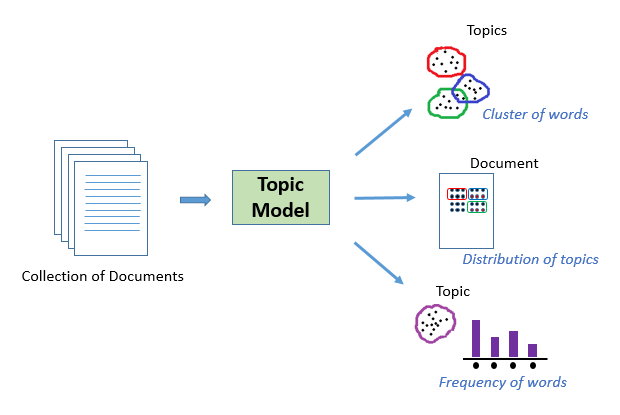
\includegraphics[width=0.7\textwidth]{figures/topic_modeling.png}
\caption{\label{fig:topic_modeling}Framework of topic modeling \citep{usmani_natural_2021}.}
\end{figure}

\begin{figure}[!h]
\centering
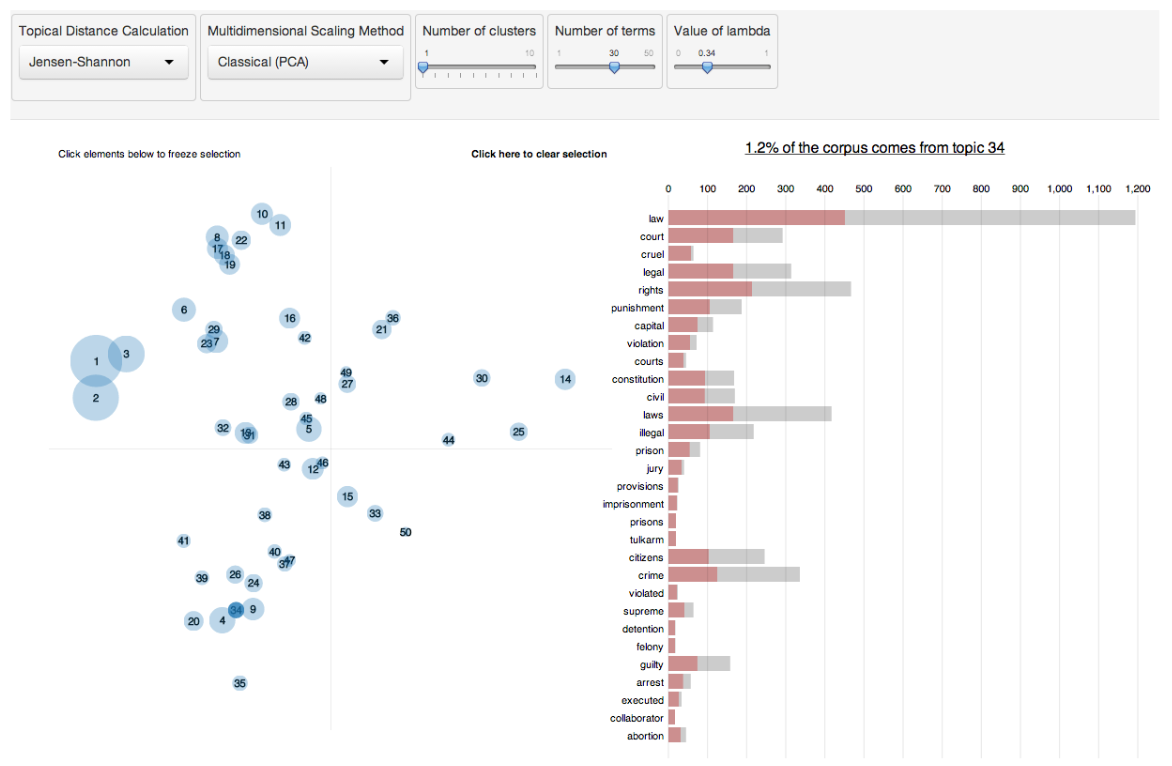
\includegraphics[width=1\textwidth]{figures/ldavis.png}
\caption{\label{fig:ldavis}The layout of LDAvis \citep{sievert_ldavis_2014}.}
\end{figure}

% ====================== | Identification of Locals and Tourists | ======================
\subsubsection{Identification of Locals and Tourists}
Distinguishing between locals and tourists is crucial when investigating how different people perceive a city. Locals and tourists might have various preferences and behaviors while visiting a city, and analyzing their patterns separately can yield valuable insights. The time interval is a commonly used indicator for identifying locals and tourists. Typically, locals are assumed to stay in the city for longer periods than tourists. Researchers have used the time interval between a user's first and last posts within a city boundary on social media platforms to estimate the length of his stay, with time intervals ranging from 10 days to 30 days \citep{girardin_digital_2008, hu_graph-based_2019, hopken_flickr_2020}. For example, given a 30-day threshold, a Twitter user whose first and last Tweets were posted within a 20-day time interval would be classified as a tourist. However, it is important to note that some locals may share content only for short periods, and some tourists may stay longer and continue sharing content. Another indicator of determining locals and tourists is user profiles. Social media platforms like Foursquare, Flickr, and Twitter, offer \acrshort{api} to collect user profiles containing information on their city of residence and hometown. Previous studies have demonstrated the feasibility of using these profiles to identify users' origins \citep{ferreira_beyond_2015, li_analyzing_2018}. However, this approach has some limitations, as many users may leave their profiles incomplete without providing the city of residence. \cite{ferreira_uncovering_2020} combined both the time interval and user profiles to overcome these limitations. If a user's time interval suggests that he is a local, but his profile indicates that he is from another city, he would be classified as a tourist. There are also other indicators for the identification of locals and tourists. In addition to the time interval, \cite{hallot_who_2015} also analyzed the categories of the place visited and the frequency of visits within the same place to extract tourists. \cite{yang_identifying_2021} assumed that locals and tourists might have different numbers of Foursquare check-ins, total travel distances, and time intervals, and applied K-means clustering to separate users into locals and tourists based on the above indicators. \cite{hasnat_identifying_2018} used the number of Tweets within the geographical boundary as an indicator to identify tourists. For example, if a user posted fewer Tweets within the geographical boundary of Florida between 12 am and 6 am than outside the boundary, he would be assumed as a local. Overall, these approaches help researchers to effectively differentiate between locals and tourists, enabling them to investigate the visiting behaviors of different groups of people.


% ============================= || Place || =============================
\subsection{Place}
% ====================== | Place Conceptualization | ======================
\subsubsection{Place Conceptualization}
\underline{definition of place, which will be used to explain why places are clusters of check-ins instead of merely check-ins}
\underline{add place studies mentioned in colloquium}

City perception can be shaped by individuals' perceptions of various places. To explore place-based perception, the first step is to conceptualize the place. According to \cite{tuan_place_1975}, place is created by human beings for human purposes, and it encompasses not only geometrical and ideographic perspectives but also an experiential perspective. It is important to distinguish between space and place. Space is defined as a continuous and unrestricted area that can be free to use or occupied, moreover, it is abstract and lacks content. While place is a segment of geographical space loaded with human meaning, offering the potential for human interaction \citep{tuan_place_1975, agnew_space_2011, cresswell_place_2014}. \cite{relph_place_1976} developed an \textit{insideness} scale to illustrate the social relationships of a place, which includes the knowledge of the physical details of place, sense of connection with a community, and a personal connection with place. Moreover, \cite{williams_measurement_2003} employed the place attachment \citep{altman_place_1992} as the scale to identify and measure the meanings of places based on the place identity \citep{proshansky_city_1978,proshansky_place_1983} and place dependence \citep{stokols_people_1981}. As the definition of place has evolved, researchers have contributed to the conceptualization of place dimensions. \cite{jorgensen_comparative_2006} described place with three dimensions: (1) place-specific beliefs (\textit{place identity}), (2) emotions (\textit{place attachment}), and (3) behavioral commitments \textit{place dependence}. \cite{agnew_space_2011} conceptualized the place with three dimensions: (1) \textit{location}, which refers to the physical position of a place represented by its name and coordinates, (2) \textit{locale}, which encompasses the properties and affordance of a place, and (3) \textit{sense of place}, which is associated with the sentiments and emotions of individuals who visit the place \citep{bahrehdar_description_2018}. It is noteworthy that according to the affordance theory, \textit{affordance} can shape behavior and guide actions of individuals \citep{gibson_theory_1977}, thus the affordance of place can influence how people perceive it. 

% ====================== | Place Dimensions Representation | ======================
The dimension \textit{location} is typically represented by the toponym. For the dimension \textit{locale}, 
\cite{wartmann_characterizing_2016,wartmann_describing_2018} have refined it with categories of landscape elements, indicating the possibility of representing this dimension with place categories. \cite{koirala_social_2015} categorized places based on tourism ontologies, which include (1) leisure, (2) restaurant, (3) attraction, (4) emergency service, (5) transport, (6) accommodation, and (7) other buildings. \cite{liu_stccd_2020} constructed a location category hierarchy tree based on daily purposes, including (1) work/study, (2) food, (3) entertainment, (4) traffic, and (5) live. \acrfull{lbs} providers also categorize places to offer place-related \acrshort{api} for users to search for \acrshort{poi} by category (Table~\ref{tab:lbs_place_categories}). However, these place categories are typically divided based on specific services provided by \acrshort{lbs} providers, and the categorization bias might lead to incomplete categories. For instance, Waze provides services for driving directions and live traffic conditions updates, which means that its place categories tend to be traffic-oriented. Tripadvisor is an online travel agency that provides guidelines for visitors, and it divides places mainly based on where to stay and what to do during a trip. To address this limitation, some studies have modified the place categories provided in \acrshort{lbs} platforms based on their research objectives. For example, in the case of Foursquare check-ins, the place category system is structured hierarchically and there are subcategories under categories. \cite{ferreira_uncovering_2020,yang_identifying_2021} improved the place categories by moving some subcategories into other categories or new categories to gain a better understanding of visitors' behaviors. The dimension \textit{sense of place} is closely linked to people's emotional attachment to the place. Conducting surveys is a way to gather information on people's emotional relationships with places and to understand their positive or negative experiences \citep{manzo_for_2005}. However, surveys can be time-consuming, and \acrshort{ugc} can provide an alternative means of exploring people's relationships with places. \cite{wang_using_2015} utilized Foursquare check-ins to evaluate the performance of four different clustering algorithms in identifying meaningful places. \cite{sui_inferring_2013} applied \acrshort{lda} to georeferenced travel blogs to generate meaningful topics describing places. \cite{hallot_who_2015} combined Google Place reviews and Foursquare check-ins to retrieve place-based semantics, enabling the inference of additional information about users based on their movements.

\begin{table}[!h]
\centering
\caption{\label{tab:lbs_place_categories}Overview of place categories in various LBS providers.}
\begin{adjustbox}{max width=\textwidth, margin=0cm}
\begin{threeparttable}
\begin{tabular}{lp{10cm}l} \hline
LBS Provider & Place Categories & Related API\\ \hline
Google Maps\tnote{a} & Airport, Amusement Park, Bank, Cafe, Embassy, Gym, Hospital, Library, Museum, Zoo, etc. (Google Maps divides places into 96 categories in total ) & Places API \\
Esri ArcGIS\tnote{b} & Arts and Entertainment, Education, Food, Land Features, Nightlife Spot, Parks and Outdoors, Professional and Other Places, Residence, Shops and Service, Travel and Transport, Water Features & Geocoding REST API \\
Foursquare\tnote{c} & Arts and Entertainment, Business and Professional Services, Community and Government, Dining and Drinking, Event, Health and Medicine, Landmarks and Outdoors, Retail, Sports and Recreation, Travel and Transportation & Places API \\
Tripadvisor\tnote{d} & Hotel, Restaurant, Attraction & Location Search API \\
Waze\tnote{e} & Parking Lot, Car Services, Transportation, Professional and Public, Shopping and Services, Food and Drink, Culture and Entertainment, Other, Lodging, Outdoors, Natural Features & Waze API \\
HERE\tnote{f} & Eat and Drink, Going Out-Entertainment, Sights and Museums, Natural and Geographical, Transport, Accommodations, Leisure and Outdoor, Shopping, Business and Services, Facilities, Areas and Buildings & Geocoding \& Search API \\
TomTom\tnote{g} & Agriculture, Beach, Castle, Factory, Garden, School, Railroad Stop, Temple, etc. (TomTom divides places into 778 categories in total ) & Category Search API \\ \hline
\end{tabular}
\footnotesize{Source: LBS provider websites as of May 2023.}
\begin{tablenotes}\footnotesize
\item[a] \url{https://www.google.com/maps}
\item[b] \url{https://www.arcgis.com/index.html}
\item[c] \url{https://foursquare.com/}
\item[d] \url{https://www.tripadvisor.com/}
\item[e] \url{https://www.waze.com/live-map/}
\item[f] \url{https://www.here.com/}
\item[g] \url{https://www.tomtom.com/}
\end{tablenotes}
\end{threeparttable}
\end{adjustbox}
\end{table}

 
% ====================== | Place Popularity Measurement Among Locals and Tourists| ======================
\subsubsection{Place Popularity Measurement Among Locals and Tourists}
The distribution of locals and tourists can provide valuable insights into the popularity of places among two groups of people. In previous studies, researchers have employed various indices to measure the patterns of population distributions. One commonly used index is the \textit{index of dissimilarity}, which was proposed by \cite{sakoda_generalized_1981} to measure the distribution of two populations across geographic areas. \cite{li_analyzing_2018} applied this index to represent the degree of mix between locals and tourists to study their spatial interactions. The \textit{index of dissimilarity} is calculated as the sum of the difference ratio of locals and tourists in each place, reflecting the overall distribution of locals and tourists over the study area. However, the difference ratio itself is also a good indicator to measure the popularity of individual places. In addition, \cite{mcelroy_applying_1993} formulated the \textit{density ratio} (the number of visitors multiplied by the average length of stay, divided by land area multiplied by 365) and the \textit{penetration ratio} (the number of visitors multiplied by the average length of stay, divided by the population multiplied by 365) to reveal the degree of tourists influx into an area. These two indices were typically used to measure the tourist carrying capacity \citep{mcelroy_applying_1993,thomas_tourist_2005}. However, the \textit{penetration ratio}, which shows the proportion of tourists in a specific place at a temporal scale, can also be used to measure the popularity of places among two groups of people. \cite{mcelroy_applying_1993,mcelroy_tourism_1998} developed the \textit{tourism penetration index} to measure the degree of tourism penetration. The calculation of \textit{tourism penetration index} involves three variables: (1) per capita visitor spending, (2) daily visitor densities per 1,000 population, and (3) hotel rooms per square kilometer, as indices to measure the tourism impact. The \textit{tourism penetration index} is then calculated as the unweighted average of the three standardized indices. In the context of place popularity measurement, the second variable, which reveals the average tourist density, also indicates the place popularity among locals and tourists, and standardizing this index helps to investigate the distribution of these two groups of people for each place. Furthermore, the \textit{tourist ratio}, calculated as the ratio of the number of tourists to the number of residents in a specific area, is also an indication of the intensity of tourist influx \citep{faulkner_framework_1997}. 


% ============================= || Semantic Trajectory || =============================
\subsection{Semantic Trajectory} \label{semantic_trajectory}

% ====================== | Semantic Trajectory Construction | ======================
\subsubsection{Trajectory Construction}
% ============== introduction to the semantic trajectory ==============
Detecting the movement patterns of visitors from their trajectories helps to understand their visiting behaviors. However, interpreting these patterns can sometimes be challenging due to the lack of contextual information. To address this, attempts have been made to integrate semantic descriptions into raw trajectories to build semantic trajectories. A trajectory can be assumed as a sequence of stops and moves \citep{spaccapietra_conceptual_2008}. Stops represent specific points along the trajectory where the moving object stays for a certain duration, typically denoting locations of interest. For instance, in tourism studies, stops could include sightseeing spots, hotels, airports, etc. \citep{yuan_review_2017}. Moves represent the transitions between stops in a trajectory, indicating the segments from one stop to the next. Unlike raw trajectories that only capture spatial or spatiotemporal properties (Figure~\ref{fig:raw_trajectory_example}), semantic trajectories enrich stops and moves with contextual data such as weather, transportation means, and place type (Figure~\ref{fig:semantic_trajectory_example}). The integration of semantic information enables the extraction of meaningful trajectory behaviors. For example, in the context of tourism, a tourist behavior can be identified if the trajectory begins and ends at an accommodation place, with several stops at museums or tourist attractions \citep{parent_semantic_2013}. Constructing a semantic trajectory involves identifying stops, which are the important places of trajectory, based on the trajectory data. Subsequently, stops or moves are annotated with semantic information, and this process is also called semantic enrichment.

\begin{figure}[!h]

\centering
\begin{subfigure}{0.5\textheight}
\centering
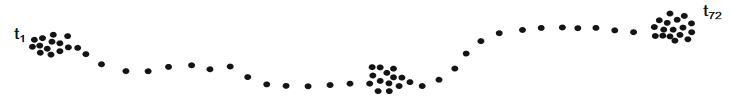
\includegraphics[width=0.9\linewidth]{figures/raw_trajectory_example.png} 
\caption{Raw trajectory.}
\label{fig:raw_trajectory_example}
\end{subfigure}
\begin{subfigure}{0.5\textheight}
\centering
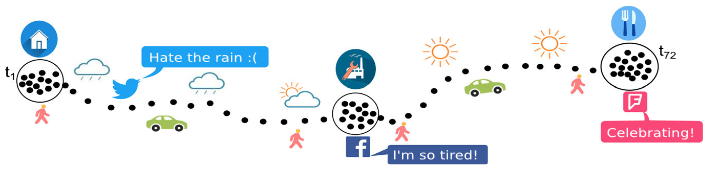
\includegraphics[width=0.9\linewidth]{figures/semantic_trajectory_example.png}
\caption{Semantic trajectory}
\label{fig:semantic_trajectory_example}
\end{subfigure}

\caption{Example of trajectories \citep{ferrero_mastermovelets_2020}.}
\label{fig:trajectory_example}
\end{figure}



% ============== GPS data ==============
\acrfull{gps} data is widely used for constructing trajectories. Various approaches exist for identifying stops from \acrshort{gps} data. One method involves detecting stops by examining the absence of \acrshort{gps} signals or when the velocity remains zero during a specific time interval \citep{ashbrook_using_2003}. However, the presence of signal errors decreases the accuracy of identifying actual stops using this technique. Alternatively, other approaches consider both the \acrshort{gps} data and background geographic information to identify stops. \cite{alvares_model_2007} developed an algorithm named SMoT (Stops and Moves of Trajectories) for extracting stops and moves. In their study, a stop is defined as a location where an object remains for a minimal amount of time, and it is annotated with the corresponding place type and timestamp. Density-based clustering algorithms are also employed to identify stops. \cite{palma_clustering-based_2008} treated stops as \acrshort{poi} and utilized various \acrshort{dbscan} algorithms to cluster points as places based on the speed between two points. To enrich trajectories with semantic enrichment, different techniques have been employed, such as semantic regions, semantic lines, and semantic points, to annotate trajectories \citep{yan_semantic_2013}. Semantic regions refer to meaningful geographic areas, such as land use, and stops in trajectories can be annotated with semantic information by considering their topological correlation with these regions. Semantic lines typically represent transportation networks, the movements within trajectories can be linked to road segments through map-matching algorithms, helping to infer the transportation mode, such as walking, driving, or using public transportation like metros. Semantic points correspond to \acrshort{poi} with meaningful place types, like restaurants, museums, and train stations. Stops in trajectories can be linked to the closest \acrshort{poi} to annotate semantic information. Furthermore, stops and moves can be annotated with activities, like staying at home, having lunch at a restaurant, or working at a company, by considering the time individuals spend at different \acrshort{poi} and their routines \cite{parent_semantic_2013}.

% ============== UGC data ==============
In addition to utilizing \acrshort{gps} data, the growing utilization of \acrshort{ugc} data shows its potential in semantic trajectory construction by providing more semantic information beyond the spatial location. Trajectories have been built using check-ins gathered from platforms like Foursquare, Gowalla, and Brightkite. In these cases, a stop is defined as a semantic \acrshort{poi} with a minimum of 10 check-ins, and consecutive check-ins within a 10-min threshold are removed as duplicates \citep{petry_towards_2019,ferrero_mastermovelets_2020}. Another approach employed by \cite{nin_tweets_2014} involved aggregating geotagged tweets to create trajectories, associating them with Foursquare categories to construct the Semantic Origin Destination Matrix of Foursquare categories. Geotagged photos from Flickr have also served as a valuable data source for building semantic trajectories. \cite{cai_mining_2018} conducted semantic trajectory clustering using geotagged photos from Flickr to mine mobility patterns. Additionally, they identified semantic regions of interest where a high density of trajectories passed, providing more meaningful descriptions of the trajectories. Similarly, \cite{yang_quantifying_2017} utilized geotagged Flickr photos to extract tourist trajectories, expanding the trajectory dimensions from topological and temporal spaces to semantic spaces. This allowed for a better understanding of travel motifs and the discovery of meaningful patterns of tourist behavior. In terms of semantic enrichment, various attributes have been employed to enrich the semantic information of trajectories, including place type, price tier, rating, day of the week, time of day, and weather information have been used to enrich semantic information for trajectories \cite{cai_mining_2018,petry_towards_2019,liu_stccd_2020,ferrero_mastermovelets_2020}. Place type is a fundamental contextual piece of information associated with semantic trajectories, which can be collected from sources such as \href{http://www.geonames.org/}{GeoNames} or represented by venue categories derived from check-ins. Studies that utilized check-ins to construct trajectories also considered the price tier and rating associated with the check-ins. These attributes, together with place type, provide additional information about the visited places. Day of the week and time of day assist in interpreting mobility patterns with greater time granularity. For instance, it is possible to identify typical trajectories where an individual commutes from home to work at 8 am, has lunch at a restaurant at 12 pm, and so on on weekdayss. The incorporation of weather information helps to capture the influence of weather conditions on individuals' movement patterns.

% ====================== | Semantic Trajectory Pattern Mining | ======================
\subsubsection{Semantic Trajectory Pattern Mining}
% ============== introduction + distance function + similarity measure ==============
The movement patterns of individuals can be mined from semantic trajectories to understand their behaviors. Two primary techniques employed for the discovery of movement patterns are clustering and classification \citep{parent_semantic_2013}. These techniques group trajectories that share similar information. The key distinction between clustering and classification is that clustering is an unsupervised learning technique, which does not rely on prior knowledge of target groups. On the other hand, classification is a supervised learning technique that requires prior knowledge to determine target groups before the learning progress. To cluster semantic trajectories, it is important to construct similarity matrix using appropriate distance measures. Various distance functions are available to measure diverse attributes. In the context of semantic trajectories, spatial distance is typically evaluated using either the Euclidean Distance function or the Haversine Distance function. The Euclidean Distance function calculates the straight-line distance between two points and is suitable for coordinates in a projected coordinate system. Conversely, the Haversine Distance function measures the great-circle distance between two points on the Earth's surface and it is suitable for latitude and longitude coordinates in a geographic coordinate system. Semantic trajectories may also encompass attributes with categorical values, such as place type and weather. For measuring the distance between such attributes, discrete distance functions like the Hamming Distance function and Jaccard Distance function are commonly employed. These functions are particularly useful for binary or categorical data, allowing for the quantification of the distance between different attribute values.

To extract typical trajectories, it is essential to measure trajectory similarity. Commonly used similarity measures for trajectories include Dynamic Time Warping (DTW) \citep{berndt_using_1994}, Multidimensional Dynamic Time Warping (MD-DTW) \citep{ten_holt_multi-dimensional_2007}, Longest Common SubSequence (LCSS) \citep{vlachos_discovering_2002}, Edit Distance (EDR) \citep{chen_robust_2005}. A comparative study of these trajectory similarity measures was conducted by \cite{tao_comparative_2021}. DTW measures the distance between time series and is specifically suitable for numerical values. It determines the optimal alignment of two sequences to identify the contiguous path with the minimum total distance between the series. However, DTW only considers one dimension. To address this limitation, MT-DTW was developed to adapt DTW for multidimensional sequences. It assigns weights to different dimensions and constructs the distance matrix for each pair of elements in the sequences by normalizing the distance values across all dimensions. Both DTW and MT-DTW have a drawback in that they are sensitive to noises, such as distant elements. LCSS, proposed as a similarity measure for raw trajectories, overcomes this limitation by introducing the distance and matching threshold to identify the longest common subsequence. If the distance between two points falls within the matching threshold, a similarity value of 1 is assigned; otherwise, a similarity value of 0 is assigned. LCSS can also be extended to measure trajectories with additional dimensions, such as semantics. EDR, derived from LCSS, also utilizes the matching threshold with binary values (0, 1) to represent the distance. It calculates the distance between trajectories by seeking the sequence with the minimum number of inserts, deletes, and replacements of points required to transform one trajectory into another. However, most trajectory similarity measures only consider a fixed number of dimensions and deal with fixed types of values. \cite{furtado_multidimensional_2016} proposed the Multidimensional Similarity Measure (MSM) to compute the similarity of trajectories with multiple dimensions, including space, time, and semantics. MSM assumes that different dimensions may have varying levels of importance in different problems, thus assigning weights to dimensions and utilizing thresholds to calculate similarity scores. This approach increases the flexibility of similarity measures. However, MSM does not consider the sequence of the movement, defining two trajectories as similar even if they visit the same place types in different orders. \cite{petry_towards_2019} developed the MUItiple-aspect TrAjectory Similarity (MUITAS) method to measure the similarity of trajectories with heterogeneous semantic dimensions. MUITAS supports different relationships among dimensions by introducing features. A feature represents a unit of analysis within a trajectory, and multiple aspects constitute the feature. Different weights can be assigned to different features based on the importance of aspects within the feature. This approach enhances the ability to capture the complexity of trajectory similarity.

% ============== semantic trajectory clustering ==============
Trajectories can be clustered using various methods, including density-based, hierarchical-based, spectral-based, and community-based trajectory clustering techniques \cite{liu_stccd_2020}. A density-based clustering method identifies clusters with high object density within a given area, enabling the detection of clusters with arbitrary shapes. One of the most renowned density-based clustering algorithms is \acrshort{dbscan}, which relies on two parameters, namely, \textit{Eps} (radius of the neighborhood) and \textit{MinPts} (minimum number of neighbors within the radius). Ordering Points To Identify the Clustering Structure (OPTICS) proposed by \cite{ankerst_optics_1999} is another density-based clustering method. OPTICS orders objects instead of clustering them as \acrshort{dbscan} does, and the ordered objects can be grouped into clusters based on the reachability distance. For instance, \cite{cai_mining_2018} applied OPTICS to cluster trajectories with multiple semantic dimensions constructed using geotagged Flickr photos, and identified semantically common trajectory patterns. In the hierarchical-based clustering approach, \cite{zhang_hierarchical_2018} proposed a hierarchical trajectory clustering method based periodic pattern mining, incorporating semantic spatiotemporal information. This method extends Traclus (Trajectory Clustering) \citep{lee_trajectory_2007} and builds upon HDBSCAN (Hierarchical Density-Based Spatial Clustering of Applications with Noise) \citep{campello_density-based_2013} to detect hierarchical clusters. Regarding community-based trajectory clustering, \cite{el_mahrsi_graph-based_2013} employed a modularity-based community detection algorithm to group frequently visited road segments from different trajectories. This approach enables the discovery of a hierarchy of nested clusters of road segments. \cite{liu_todmis_2013} proposed Trajectory cOmmunity Discovery using Multiple Information Sources (TODMIS) to mine communities from trajectories, which combines additional information, such as velocity and semantics, with raw trajectories and applied dense sub-graph detection to discover the set of distinct communities.


% ============== semantic trajectory classification ==============
Classification is a process that groups similar trajectories into predefined classes. In the context of semantic trajectories, \cite{lee_trajectory_2007} initially clustered interesting line segments derived from trajectories. Subsequently, they assigned a class to each cluster and classified other trajectories by placing them into these predefined classes. To delve into the analysis of trajectory data, \cite{giannotti_unveiling_2011} developed M-Atlas, a comprehensive system that facilitates the exploration of both raw and semantic clustering and classification, and discovered human mobility through querying and mining trajectory data. Within their study, trajectories were clustered, and new trajectories were classified by assigning them to the identified clusters. \cite{ferrero_mastermovelets_2020} introduced a new parameter-free method known as MasterMovelets. This approach identifies the most relevant sub-trajectories while considering various combinations of dimensions. By leveraging this method, trajectory classification can be achieved efficiently and effectively. 

% ============== sequential pattern mining ==============
Clustering and classification techniques are employed to group semantic trajectories that share similar attributes. In addition to these methods, sequential pattern mining serves as a complementary approach to extract frequently occurring mobility patterns within trajectories. Sequential pattern mining allows for the occurrence of frequent points in a specific temporal order, which means that each point can occur multiple times as long as it is visited several times during the same period. One of the pioneering algorithms in sequential pattern mining is the Generalized Sequential Patterns (GSP) algorithm proposed by \cite{srikant_mining_1996}. This algorithm accommodates the specification of (1) time constraints between adjacent elements of the sequential pattern, (2) sliding time windows of the transaction, and (3) user-defined taxonomies. In the study conducted by \cite{hopken_flickr_2020}, the GSP algorithm was applied to identify behavioral patterns of tourists using Flickr data. The authors compared the typical trajectories mined through association rule analysis and sequential pattern mining. \cite{pei_mining_2004} introduced a \acrfull{prefixspan} algorithm to mine sequential patterns through a pattern-growth approach, which consumes less memory space than GSP. Furthermore, \cite{yin_diversified_2011} applied the \acrshort{prefixspan} method to discover the trajectory patterns of Flickr users. They also employed various ranking methods to find top-ranked patterns based on different criteria.

% ============================= || Research Gaps || =============================
\subsection{Research Gaps}
City perception can be investigated at different scales, such as grid-based or \acrshort{aoi}-based, but there is limited research exploring how the perception of a city can be understood through trajectories. Previous studies have demonstrated the feasibility of constructing trajectories with \acrshort{ugc} data. While geotagged social media data like Tweets, Flickr photos, and Foursquare check-ins, have been utilized to build trajectories, there is a lack of research that integrates \acrshort{ugc} data as semantic information for trajectory construction and the study of city perception. Most studies directly assign information extracted from \acrshort{ugc} data, such as place type, rating, and price tier, to trajectories as the semantic dimension. However, \acrshort{ugc} also contains latent information which requires additional techniques for extraction. This study assumes that a place can be characterized by three dimensions: location, locale, and sense of place. It integrates these dimensions into the construction of semantic trajectories and enriches them through direct information assignment and topic modeling. For the construction of semantic trajectories, existing approaches are not fully suitable for exploring perception from a place-based perspective. Additionally, city perception varies among different groups of people and over different time spans, making it worthwhile to analyze more precise city perceptions comparatively. To capture the semantic information in trajectories, this study leverages \acrshort{ugc} data and integrates the place dimensions, aiming to identify the movement patterns of both locals and tourists over different time spans. By incorporating \acrshort{ugc} data, this study seeks to provide insights into city perception from a holistic and nuanced perspective.

\clearpage

% ============================================ ||| Study Area and Data Preprocessing ||| ============================================
\section{Study Area and Data Preprocessing}
\subsection{Study Area}
The study area is located in Greater London in Great Britain (Figure~\ref{fig:study_area}). As an English-speaking
city, Greater London covers an area of 1,572 \(km^2\) and has a population of 9.5 million inhabitants. According to tourism statistics of City of London, before the Covid-19 pandemic, Greater London attracted approximately 21 million visitors annually from across the world. Of these, 19.7 million visitors were day trippers, while 1.3 million visitors stayed overnight. The high volume of visitors makes Greater London an ideal location for studying the city perception of both locals and tourists. The boundary of Greater London used in this study was obtained from LONDON DATASTORE website \footnote{\url{https://data.london.gov.uk/dataset/statistical-gis-boundary-files-london}}.

\begin{figure}[h!]
\centering
\includegraphics[width=1\textwidth]{figures/study_area.png}
\caption{\label{fig:study_area}Study area.}
\end{figure}

\subsection{Data Preprocssing} \label{data_preprocessing}
Foursquare check-ins and Flickr tags in Greater London from April 3, 2012 to September 16, 2013 were collected to investigate how people move around the city and how they perceive it.

This study examines the city perceptions of locals and tourists, during the daytime and nighttime, as well as on weekdays and weekends. Therefore, it is crucial to differentiate between these two population groups across different time spans. To distinguish between locals and tourists, a combination of user profiles and time intervals was utilized for identification. The user profile served as the primary criterion, with individuals whose hometown or city of residence listed as London in their profiles categorized as locals. In cases where the user profile was unavailable, the time interval between the user's initial and final Foursquare or Flickr posts in Greater London was employed. Users with a time interval exceeding 30 days were classified as locals. Regarding time spans, daytime is defined as 6 am to 6 pm, while the remaining hours are considered nighttime. Weekdays encompass Monday to Friday, while the weekend comprises Saturday and Sunday.

\subsubsection{Foursquare Data}
Foursquare is a platform for users to check in at venues and share their experiences through reviews. As of 2022, Foursquare has more than 55 million monthly active users worldwide. The Foursquare data used in this study was obtained from the Global-scale Check-in Dataset \cite{yang_nationtelescope_2015}, containing two datasets: (1) Foursquare check-ins and (2) Foursquare \acrshort{poi} from April 3, 2012 to September 16, 2013, on a global scale.

For the dataset Foursquare check-ins, a total of 187,336 check-ins shared by 9,717 users in Greater London were extracted. This dataset includes the following fields:
\begin{itemize}
    \item User ID
    \item Venue ID
    \item UTC time
    \item Timezone offset
\end{itemize}

Another dataset Foursquare \acrshort{poi} stored Foursquare venues, and there were 27,608 \acrshort{poi} in Greater London. This dataset contains the following fields:
\begin{itemize}
    \item Venue ID
    \item Venue category name
    \item Coordinates
    \item Country code
\end{itemize}


Foursquare check-ins were merged with Foursquare \acrshort{poi} by the venue ID to get the coordinates of venues. The merged Foursquare data should be further cleaned and differentiated as either locals or tourists, and the preprocessing steps were as follows:
\begin{enumerate}
    \item Merged check-ins with \acrshort{poi} to get the coordinates for each check-in.
    \item Removed duplicated check-ins.
    \item Updated venue categories of check-ins based on the Foursquare category \footnote{\url{http://foursquare-categories.herokuapp.com/}}. The Foursquare category system uses a three-level hierarchy. For example, the Arts \& Entertainment first-level category includes a second-level category called Movie Theater, which in turn contains three third-level categories: Drive-in Theater, Indie Movie Theater, and Multiplex. This study kept only the first-level categories to represent 
    check-ins.
    \item Removed check-ins that were labeled as Residence to protect the privacy of Foursquare users.
    \item Removed users whose total travel distances are less than one kilometer. This study aims to investigate city perception through the analysis of trajectories. As such, trajectories with short travel distances are considered unsuitable for discovering meaningful patterns of city perception. Therefore, users with short travel distances were removed.
    \item Identified locals and tourists based on the number of days spent in Greater London, total travel distances, and user profiles. Users who spent more than 30 days in Greater London and had a total travel distance greater than 100 km were considered locals. For the remaining users, those who listed London as their hometown in their profiles were also categorized as locals. The user profiles were retrieved using Get User Details \footnote{\url{https://location.foursquare.com/developer/reference/v2-users-user_id}} provided by Foursquare API.
\end{enumerate}

After all these steps, a total of 177,207 check-ins by 7,183 users in Greater London were left. Out of these users, 1,087 were identified as locals and they posted 109,558 check-ins, which was far more than the number of check-ins posted by tourists, who amounted to 6,096, but posted only 67,649 check-ins (Table~\ref{tab:foursquare_summary}). Figure~\ref{fig:foursquare_distribution} shows the distribution of Foursquare check-ins, and most check-ins were concentrated in the central area of Greater London. Moreover, compared with tourists, locals tended to share more check-ins in peripheral areas.

\begin{table}[h!]
\centering
\caption{\label{tab:foursquare_summary}Summary of Foursquare data.}
\begin{tabular}{llll} \hline
Time & Population group & No. of users & No. of check-ins \\
\hline
\multirow{3}{*}{Overall} 
& All Users & 7,183 & 177,207 \\
& Locals & 1,087 & 109,558 \\
& Tourists & 6,096 & 67,649 \\
\hline
\multirow{3}{*}{Daytime} 
& All Users & 7,055 & 141,353 \\
& Locals & 1,082 & 87,803 \\
& Tourists & 5,973 & 53,550 \\
\hline
\multirow{3}{*}{Nighttime} 
& All Users & 4,932 & 33,256 \\
& Locals & 1,018 & 20,469 \\
& Tourists & 3,914 & 12,787 \\
\hline
\multirow{3}{*}{Weekday} 
& All Users & 6,692 & 128,797 \\
& Locals & 1,072 & 81,677 \\
& Tourists & 5,620 & 47,120 \\
\hline
\multirow{3}{*}{Weekend} 
& All Users & 5,174 & 45,812 \\
& Locals & 1,022 & 26,595 \\
& Tourists & 4,152 & 19,217 \\
\hline
\end{tabular}
\end{table}


\begin{figure}[h!]
\centering
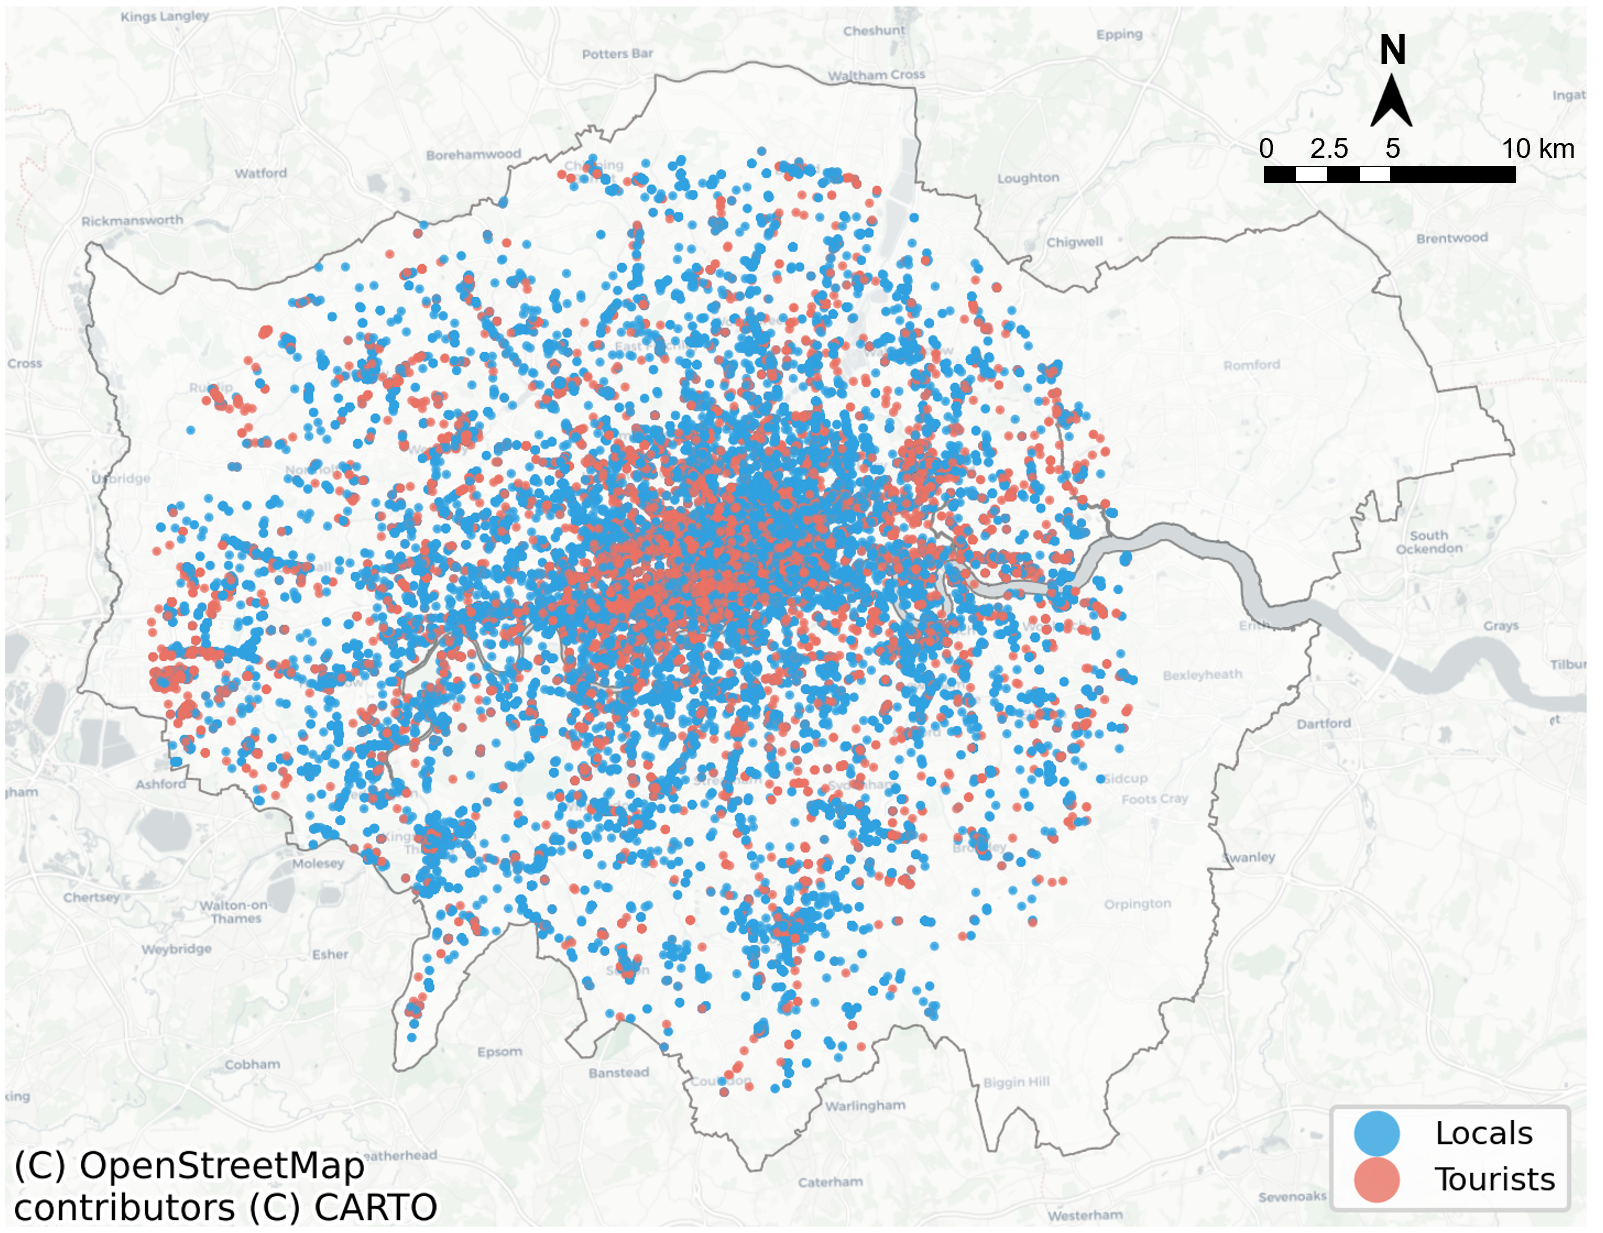
\includegraphics[width=0.7\textwidth]{figures/foursquare_distribution.png}
\caption{\label{fig:foursquare_distribution}Distribution of Foursquare check-ins of locals and tourists.}
\end{figure}

For venue categories, Foursquare categorizes the place types into ten categories, namely (1) Travel \& Transport, (2) Food, (3) Professional \& Other Places, (4) Outdoors \& Recreation, (5) Shop \& Service, (6) Nightlife Spot, (7) Arts \& Entertainment, (8) College \& University, (9) Event, (10) Residence. Category 9 Event was not contained in the check-ins used in this study, and Category 10 Residence was removed to protect the privacy of users. The number of check-ins for each Foursquare venue category is shown in Table~\ref{tab:foursquare_category}. There are several combined categories in the Foursquare category system, such as Professional \& Other Places and Outdoors \& Recreation, which makes it ambiguous to determine the visiting purposes of individual check-ins. To overcome this limitation and investigate place properties more precisely, this study divided venues into 11 categories by separating the combined categories and defining new ones based on the third-level categories in the Foursquare category system. The number of check-ins for modified venue categories is presented in Table~\ref{tab:modified_category}. In terms of the category distribution among locals and tourists, the categories transportation and Restaurant were the most prevalent among both locals and tourists. However, certain categories showed a higher prevalence among a specific group, for instance, Shopping Place, Art Place, and Accommodation were more welcomed by tourists, whereas Sports Place received a greater number of check-ins from locals (Figure~\ref{fig:foursquare_category}).

\begin{table}[h!]
\centering
\caption{\label{tab:foursquare_category}Foursquare venue category.}
\begin{tabular}{lll} \hline
No. & Foursquare venue category & No. of check-ins \\ \hline
1 & Travel \& transportation & 43,051 \\
2 & Food & 34,376 \\
3 & Professional \& Other Places & 22,184 \\
4 & Outdoors \& Recreation & 20,429 \\
5 & Shop \& Service & 19,772 \\
6 & Nightlife Spot \& Service & 18,418 \\
7 & Arts \& Entertainment & 14,285 \\
8 & College \& University & 4,692 \\ \hline
\end{tabular}
\end{table}


\begin{table}[h!]
\centering
\caption{\label{tab:modified_category}Modified Foursquare venue category.}
\begin{adjustbox}{max width=\textwidth, margin=0cm}
\begin{tabular}{lllp{6cm}p{5cm}} \hline
No. & Modified venue category & No. of check-ins & Foursquare venue category 
& Example \\ \hline
1 & transportation & 36,994 & Travel \& transportation & Airport, Train Station, Bus Station, etc. \\
2 & Restaurant & 34,376 & Food & Sandwich Place, Asian Restaurant, Italian Restaurant, etc. \\
3 & Professional Place & 29,118 & Professional \& Other Places, College \& University & Office, Government Building, Police Station, etc. \\
4 & Entertainment Place & 22,434 & Arts \& Entertainment, Shop \& Service, Nightlife Spot & Casino, Bowling Alley, Zoo, Bar, Nightclub, etc. \\
5 & Shopping Place & 18,127 & Shop \& Service & Outlet Mall, Clothing Store, Market, etc. \\
6 & Art Place & 11,132 & Arts \& Entertainment, Outdoors \& Recreation & Museum, Movie Theater, Art Gallery, Music Venue, etc. \\
7 & Green \& Blue Space & 8,220 & Outdoors \& Recreation & Park, Plaza, Garden, Lake, etc. \\
8 & Accommodation Place & 5,902 & Travel \& transportation & Hotel \\
9 & Sports Place & 5,852 & Outdoors \& Recreation & Athletics \& Sports, Pool, Playground, etc. \\
10 & Others & 3,346 & Outdoors \& Recreation, Professional \& Other Places, Travel \& transportation & Building, Bridge, Well, etc. \\
11 & Service Place & 1,706 & Travel \& Transport, Shop \& Service & Bank, Drugstore, Car Wash, Laundry Service, etc. \\ \hline
\end{tabular}
\end{adjustbox}
\end{table}


\begin{figure}[h!]
\centering
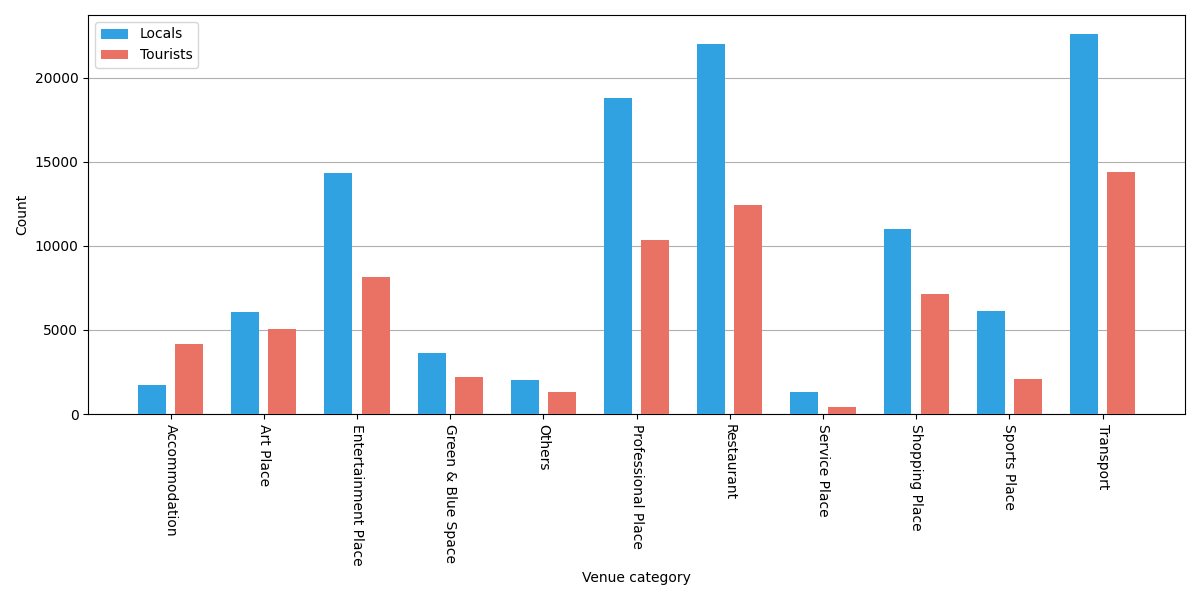
\includegraphics[width=0.9\textwidth]{figures/foursquare_category.png}
\caption{\label{fig:foursquare_category}Number of venue categories visited by locals and tourists.}
\end{figure}



\subsubsection{Flickr Data} \label{preprocess_flickr}
Flickr is an online photo management and sharing application where users can upload photos. As of 2023, the Flickr community has shared tens of billions of photos. Flickr data was collected via Flickr API with the Python library flickrapi \footnote{\url{https://stuvel.eu/software/flickrapi/}}. To collect Flickr photos, the method flickr.photos.search \footnote{\url{https://www.flickr.com/services/api/flickr.photos.search.html}} was applied to get photos. A total of 954,260 photos with unique 250,254 tags uploaded by 28,633 users in Greater London from April 3, 2012 to September 16, 2013 were collected. The main fields of Flickr data include:
\begin{itemize}
    \item Photo ID
    \item User ID
    \item Date taken
    \item Accuracy
    \item Coordinates
    \item Tags
    \item Title
    \item Photo URL
    \item Number of views
\end{itemize}

The Flickr data required additional cleaning and identification of locals and tourists. The preprocessing steps were as follows:
\begin{enumerate}
    \item Removed photos without tags because Flickr tags were one of the main semantic information in this study.
    \item Removed photos with an accuracy level below 14. Flickr divides the accuracy level on a scale of 1 to 16, with 1 representing world-level accuracy, 2-3 representing country-level accuracy, 4-6 representing region-level accuracy, 7-11 representing city-level accuracy, and 12-16 representing street-level accuracy. Only photos with an accuracy greater than 14 were kept in this study.
    \item Removed tags that were non-Ascii characters, special characters, numbers, stop-word (e.g., a, an, the), prepositions (e.g., from, to), general place names (e.g., britain, uk, england, london), and other irrelevant tags (e.g., nikon, samsung, instagram, flickr).
    \item Removed duplicates. Duplicated tags in the same list were removed. Moreover, duplicated photos of the same user at the same location with the same tags were removed.
    \item Removed prolific and unprolific users. Prolific users were defined as those who contributed more than 5\% of all photos in the dataset, while unprolific users were defined as those who uploaded less than five photos in total per day.
    \item Removed tags with a coefficient of variation greater than 300 to reduce the contribution bias. Some tags were dominantly used by prolific users, which might lead to distortions of tags. The coefficient of variation measures whether a tag is evenly used among prolific and unprolific users \cite{hollenstein_exploring_2010}. To determine the coefficient of variation, the Flickr photos were sorted based on user contribution, with the most prolific users' photos at the top. Subsequently, all photos were equally distributed into 100 bins. For each tag, a tag profile was constructed, which stored its frequency in each of the 100 bins. The coefficient of variation was calculated as the ratio of the standard deviation to the mean of the tag frequencies in the 100 bins. The lower the coefficient of variation, the more evenly the tag is distributed. For instance, based on the histogram that displays the number of photos with a certain tag in a user distribution order, the tag \textit{square} with a coefficient of variation less than 300 is more evenly distributed than the tag \textit{forms} with a coefficient of variation greater than 300.
    \item Removed tags that were place names in Greater London. GeoNames offers Free Gazetteer Data \footnote{\url{http://download.geonames.org/export/dump/}} that includes place names in Great Britain. Place names in Greater London were filtered out from the downloaded data, and any tag that matched with these place names was removed.
    \item Identified locals and tourists based on the number of days spent in Greater London and user profiles. This study used flickr.profile.getProfile \footnote{\url{https://www.flickr.com/services/api/flickr.profile.getProfile.html}} provided by Flickr API to collect user profiles, which contained information about the users' hometowns and cities. Users who had stayed in Greater London for more than 30 days were considered locals. For the remaining users, this study would also flag them as locals if their hometown or city in their profiles was listed as London.
\end{enumerate}

\begin{figure}[h!]
\centering
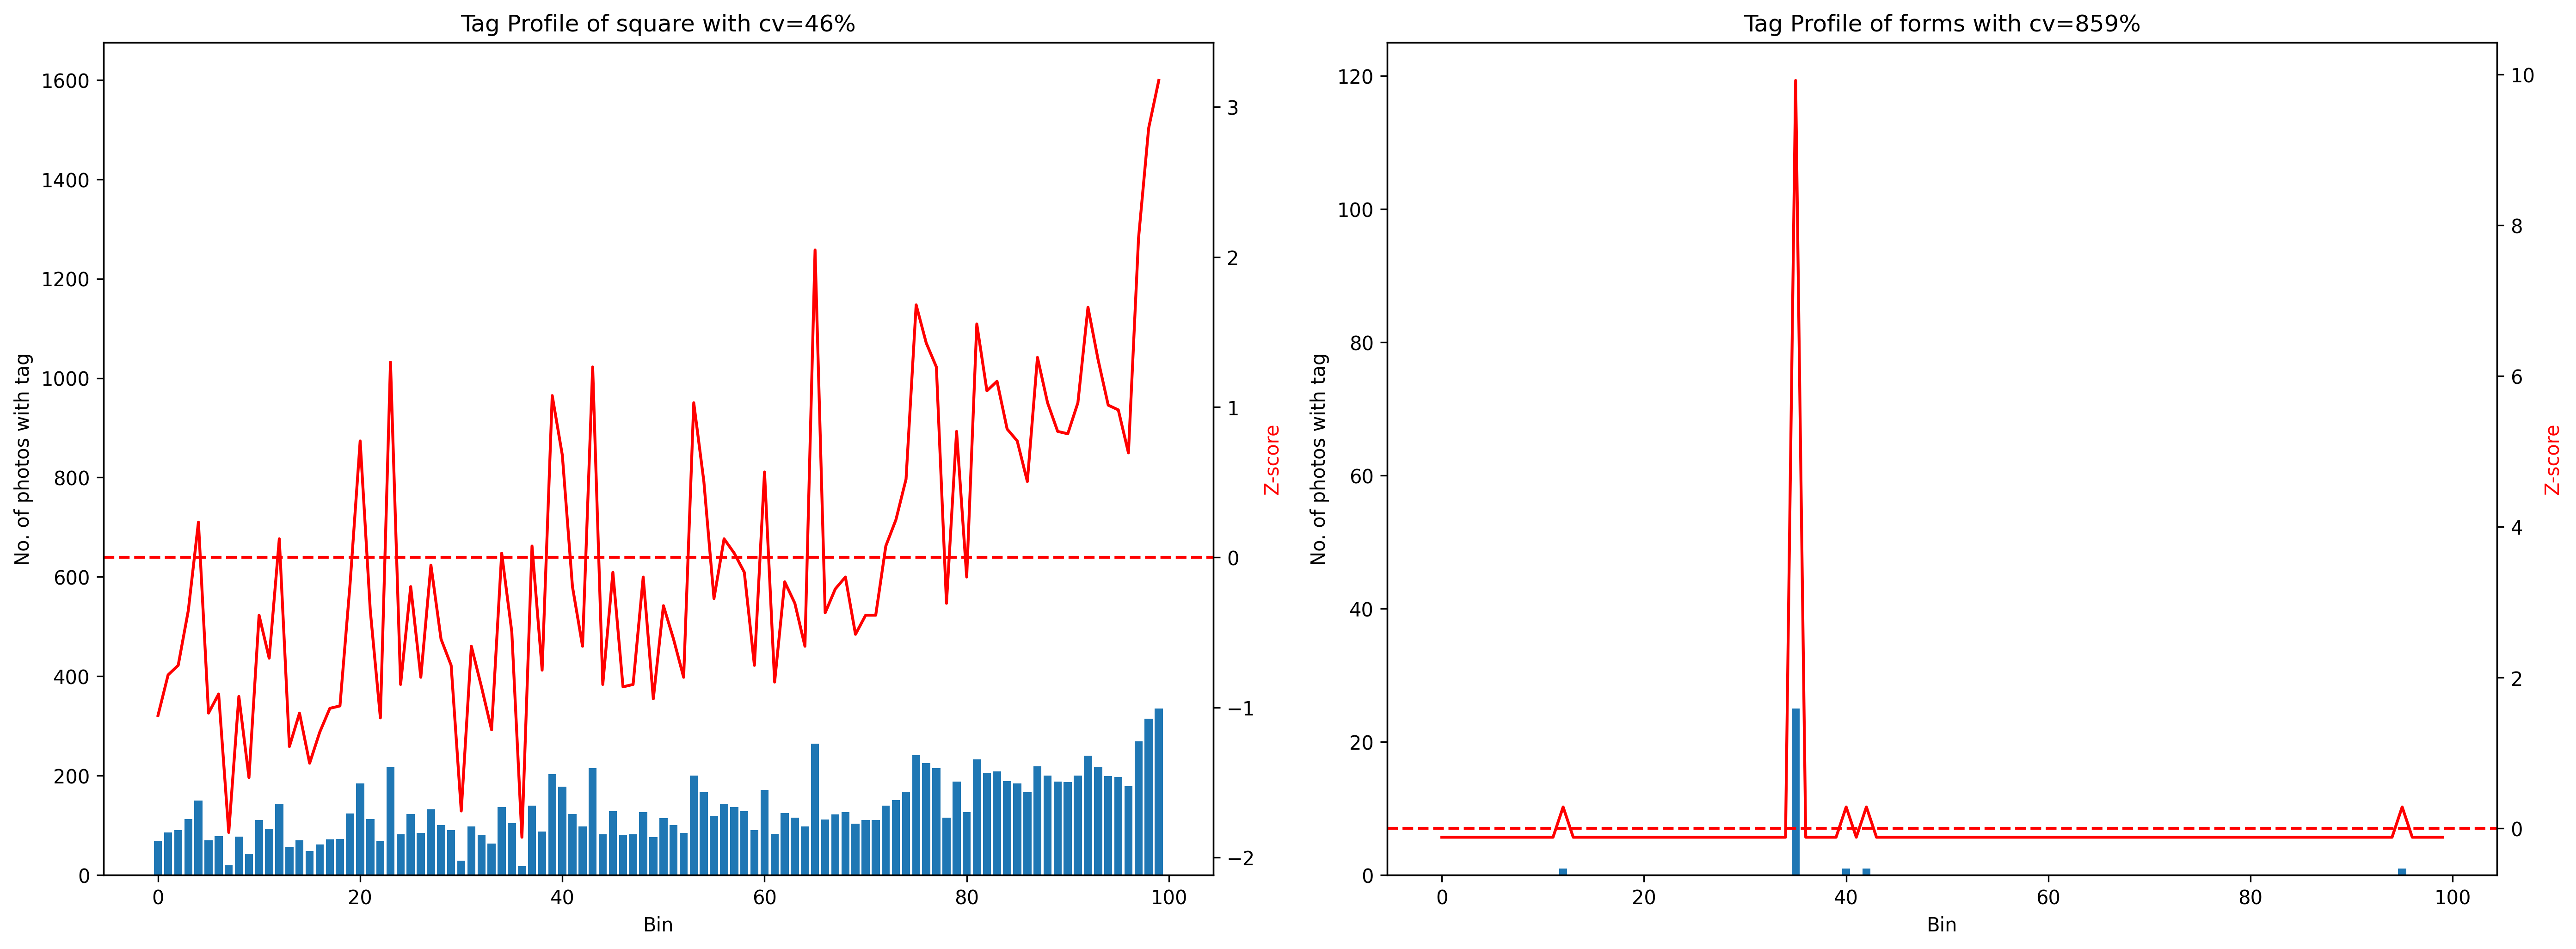
\includegraphics[width=1\textwidth]{figures/flickr_tags_cv.png}
\caption{\label{fig:flickr_tags_cv}Tag profiles.}
\end{figure}

After all these steps, 177,568 photos were left with a total of 717,747 tags (3,365 unique tags). These tags were used by 4,687 users, with 851 locals and 3,836 tourists uploading 259,967 and 457,780 tags respectively (Table~\ref{tab:flickr_summary}). The distribution of Flickr photos indicates that the majority of photos were taken in the center of Greater London, while tourists tended to share more photos around Heathrow Airport (Figure~\ref{fig:flickr_distribution}). The word cloud in Figure~\ref{fig:flickr_tag_cloud} illustrates the most frequently used tags, including city, architecture, street, park, and art.


\begin{table}[h!]
\centering
\caption{\label{tab:flickr_summary}Summary of Flickr data.}
\begin{tabular}{lllll} \hline
Time & Population group & No. of users & No. of photos & No. of tags \\
\hline
\multirow{3}{*}{Overall} 
& All Users & 4,687 & 177,568 & 717,747 \\
& Locals & 851 & 65,403 & 259,967 \\
& Tourists & 3,836 & 112,165 & 457,780 \\
\hline
\multirow{3}{*}{Daytime} 
& All Users & 4,254 & 144,748 & 580,753 \\
& Locals & 768 & 52,908 & 206,737 \\
& Tourists & 3,486 & 91,840 & 374,016 \\
\hline
\multirow{3}{*}{Nighttime} 
& All Users & 2,372 & 32,820 & 136,994 \\
& Locals & 479 & 12,495 & 53,230 \\
& Tourists & 1,893 & 20,325 & 83,764 \\
\hline
\multirow{3}{*}{Weekday} 
& All Users & 3,307 & 94,167 & 378,574 \\
& Locals & 618 & 34,243 & 132,779 \\
& Tourists & 2,689 & 59,924 & 245,795 \\
\hline
\multirow{3}{*}{Weekend} 
& All Users & 2,755 & 83,401 & 339,173 \\
& Locals & 592 & 31,160 & 127,188 \\
& Tourists & 2,163 & 52,241 & 211,985 \\
\hline
\end{tabular}
\end{table}

\begin{figure}[h!]
\centering
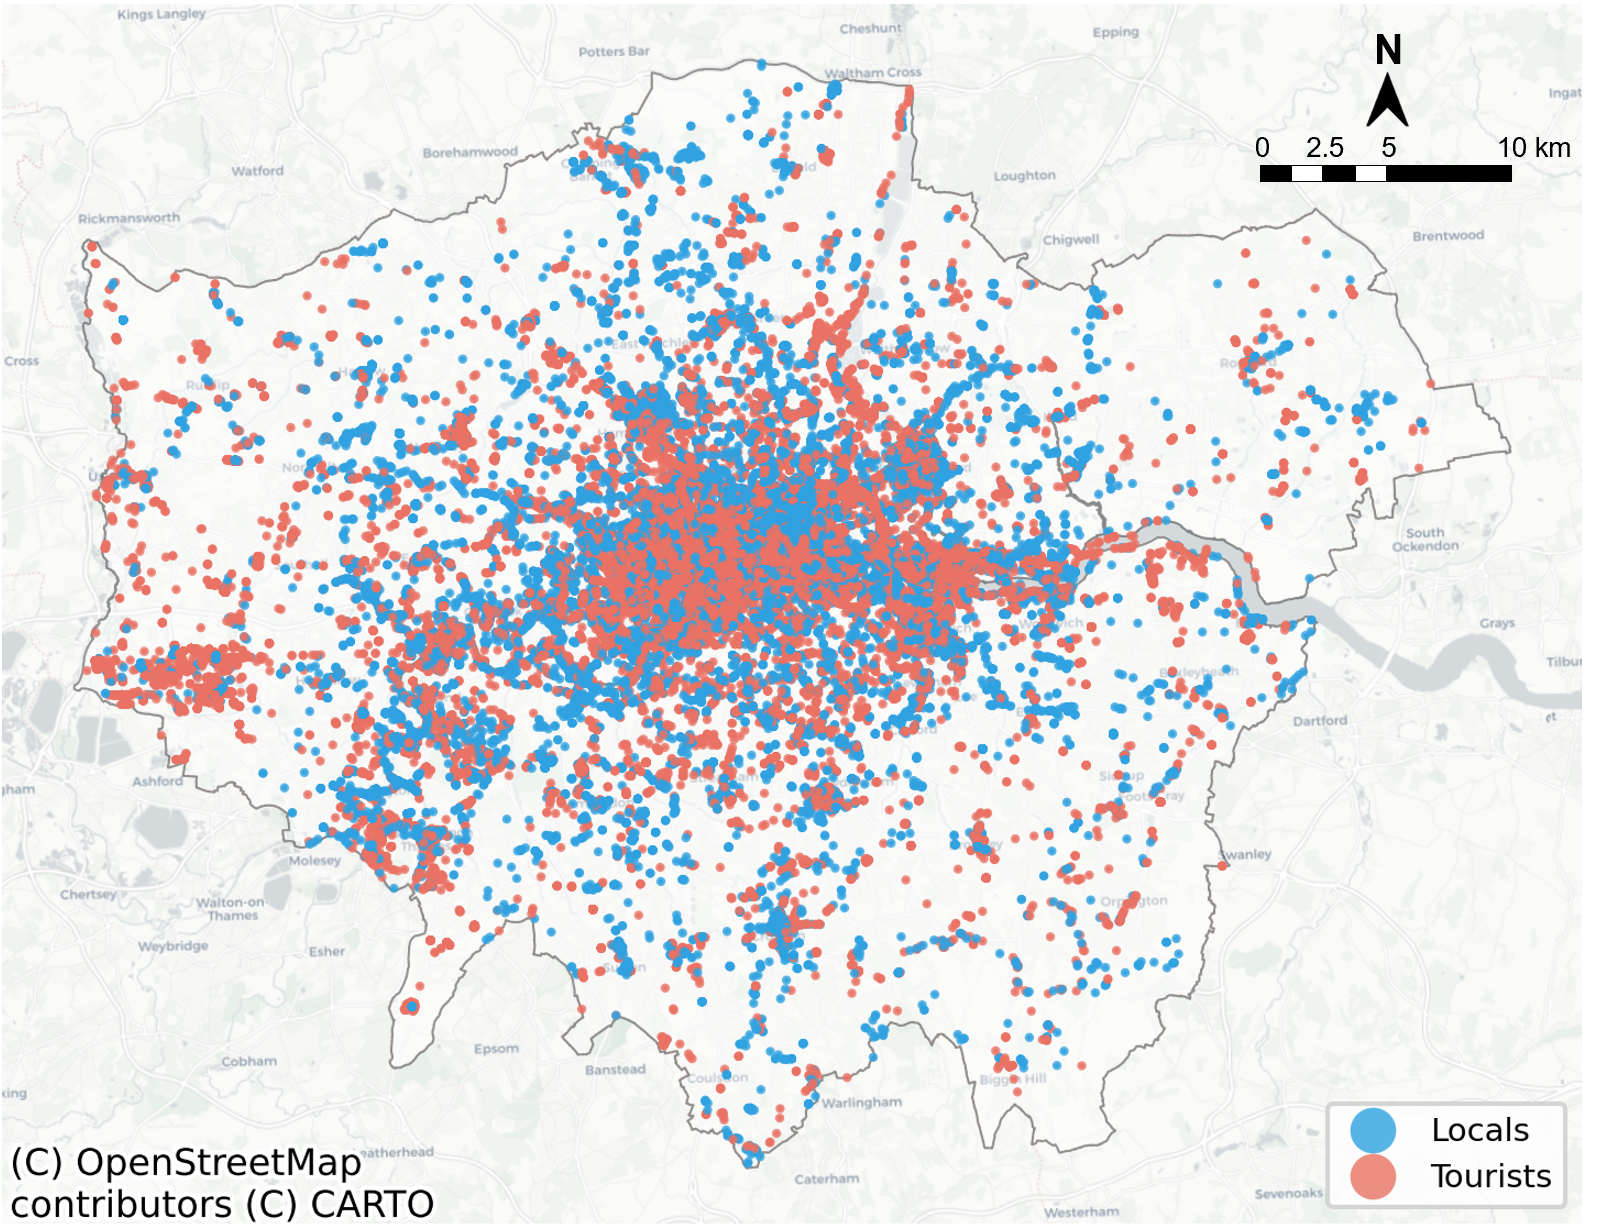
\includegraphics[width=0.7\textwidth]{figures/flickr_distribution.png}
\caption{\label{fig:flickr_distribution}Distribution of Flickr photos of locals and tourists.}
\end{figure}

\begin{figure}[h!]
\centering
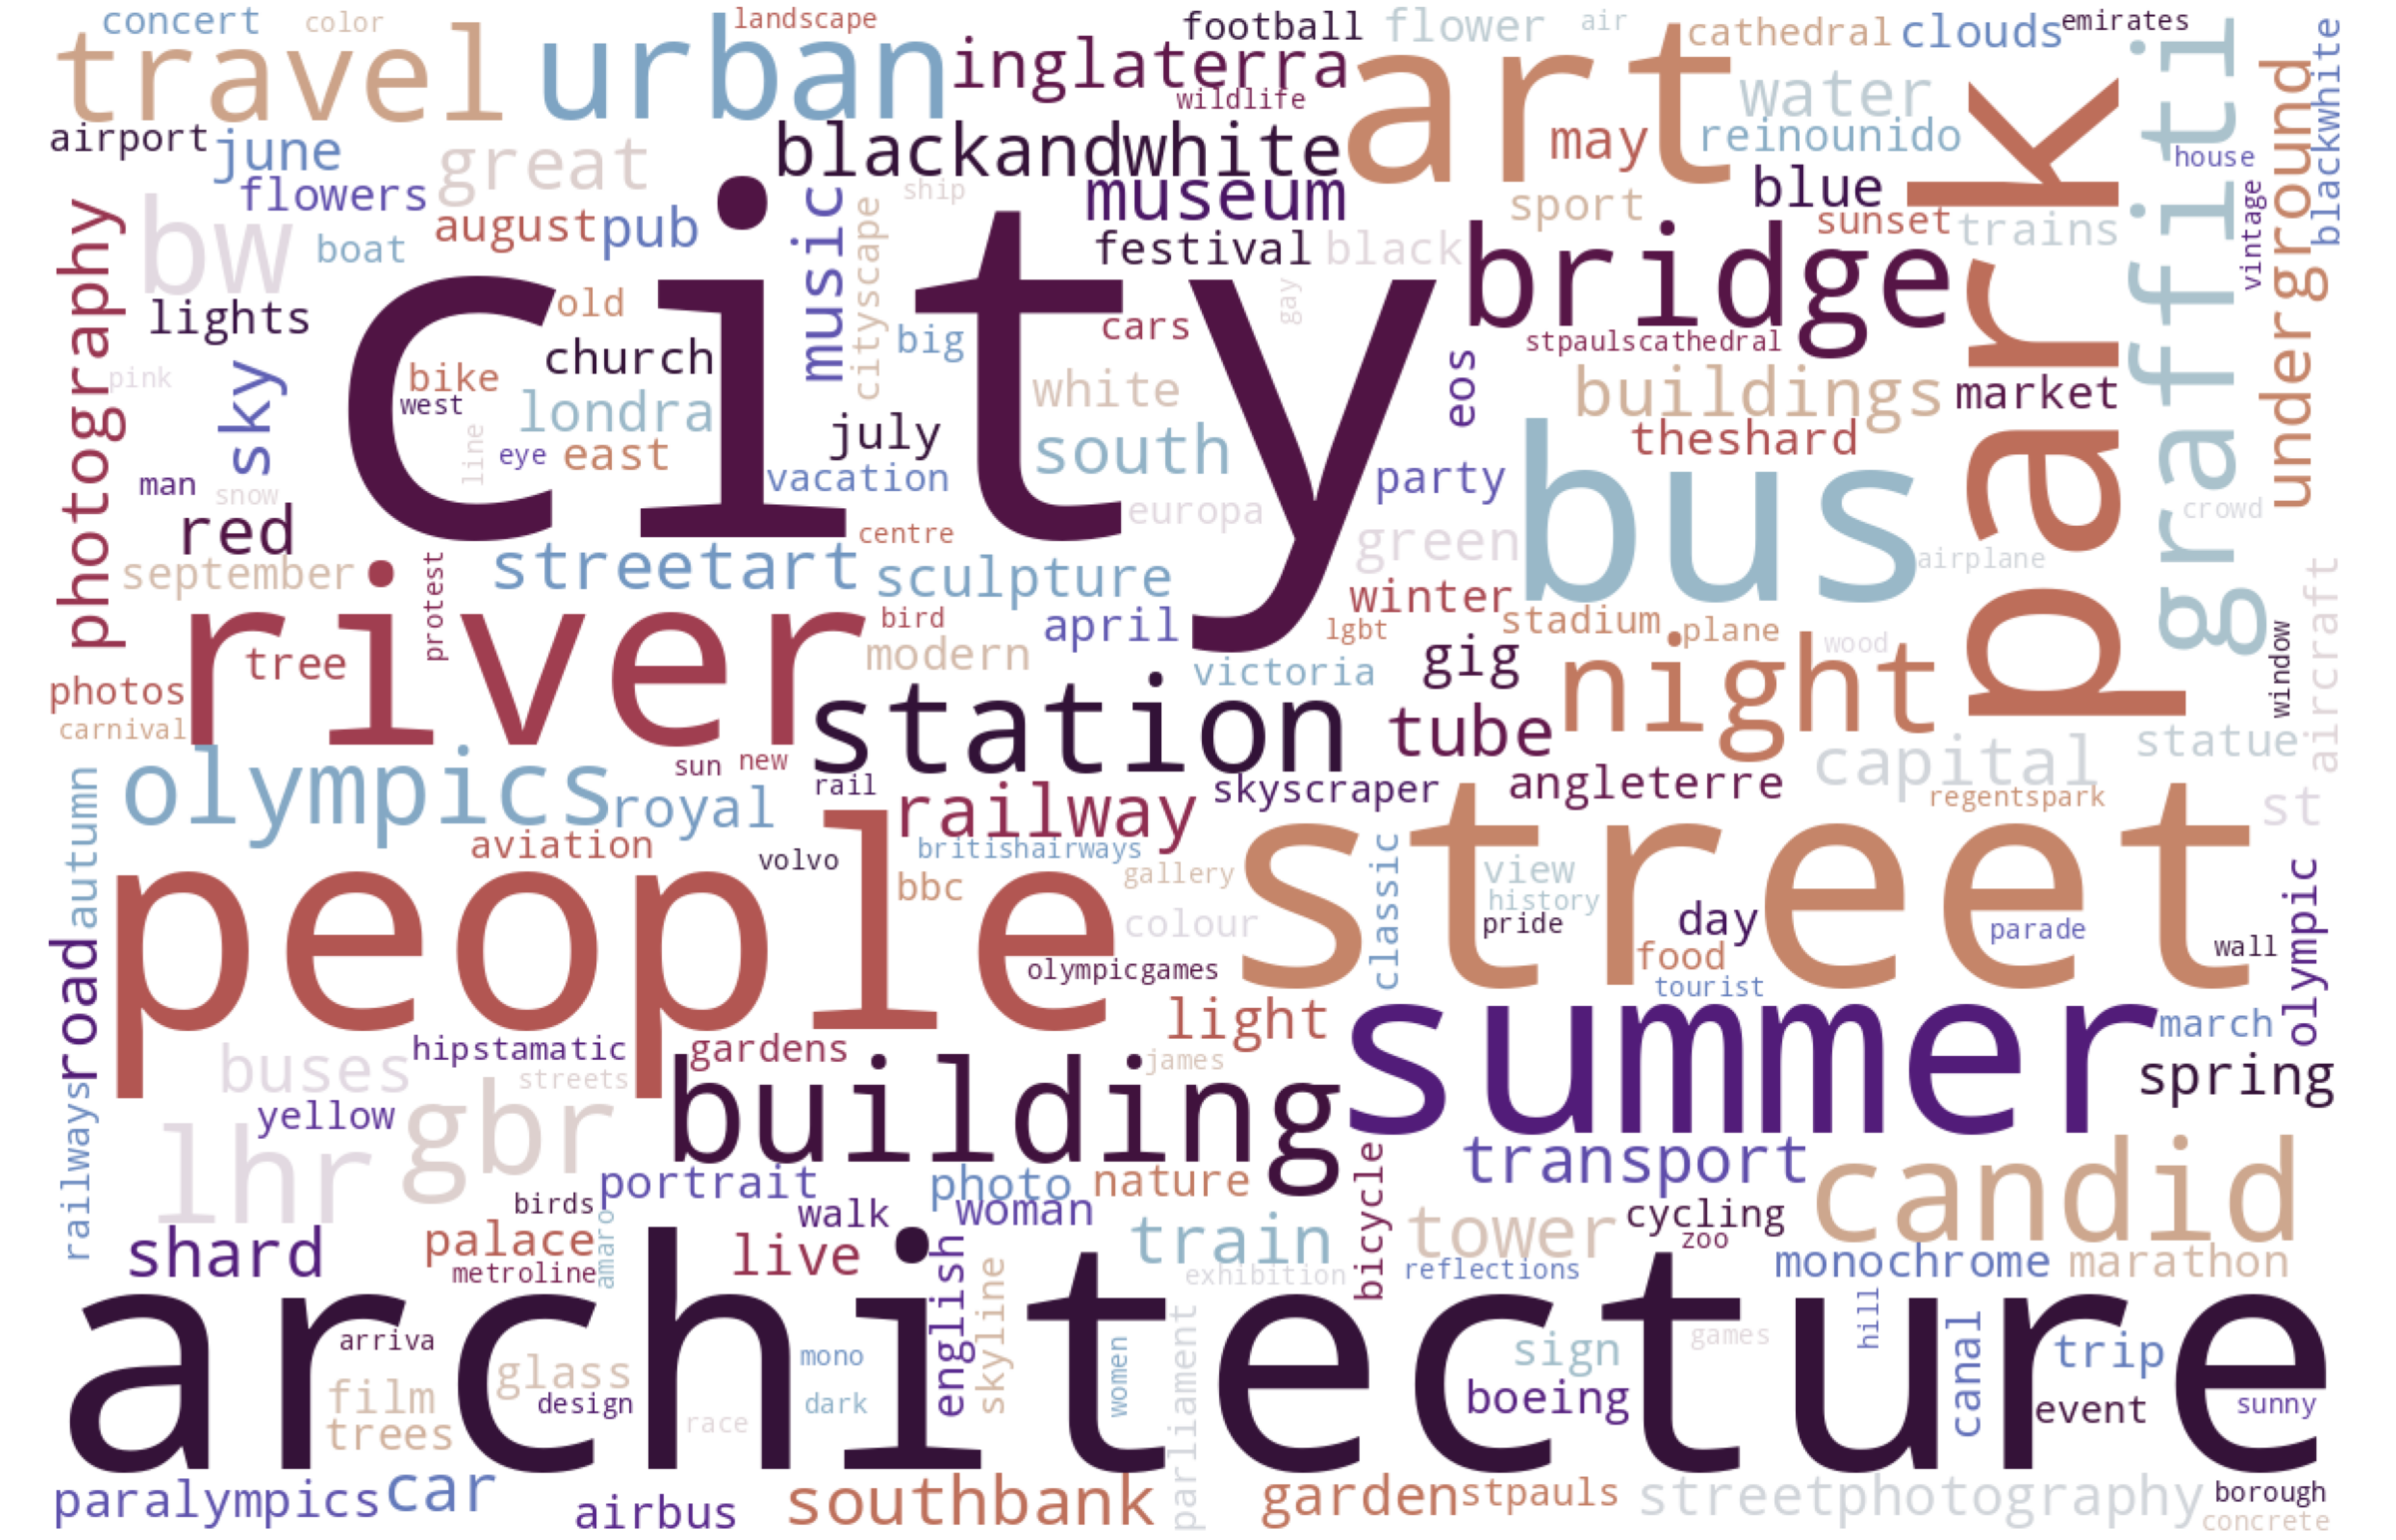
\includegraphics[width=0.7\textwidth]{figures/flickr_tag_cloud.png}
\caption{\label{fig:flickr_tag_cloud}Flickr tag cloud.}
\end{figure}


\clearpage


% ============================================ ||| Methodology ||| ============================================
\section{Methodology}
\underline{introduce this chapter}

% ============================= || Overview || =============================
\subsection{Overview}
The workflow of this study is illustrated in Figure~\ref{fig:workflow}. To explore the city perception, Foursquare check-ins and Flickr tags were utilized, and the process of data preprocessing is elaborated in Section \ref{data_preprocessing}. This workflow is designed to address two research questions. The first research question was answered by employing the methods discussed in Section \ref{hotspots_detection}, which involved identifying hotspots of locals and tourists by applying \acrfull{kde} to their Foursquare check-ins. To investigate the popularity of specific areas among locals or tourists, the difference ratio between these two groups of people was calculated and visualized in rasters. For the second research question, the construction of semantic trajectories was necessary. Prior to the trajectory construction, the Place was modeled and enriched with semantic information based on its dimensions (Section \ref{place_modeling}). Subsequently, semantic trajectories were clustered, and typical semantic trajectories of each cluster were extracted through sequential pattern mining (Section \ref{typical_semantic_trajectory_mining}). These two research questions were investigated under eight scenes to compare the popular areas and city perception among locals and tourists across different time spans, as illustrated in Figure~\ref{fig:scene}. This study was conducted with Python 3.10.12 \footnote{\url{https://www.python.org/downloads/release/python-31012/}}.


\begin{figure}[h!]
\centering
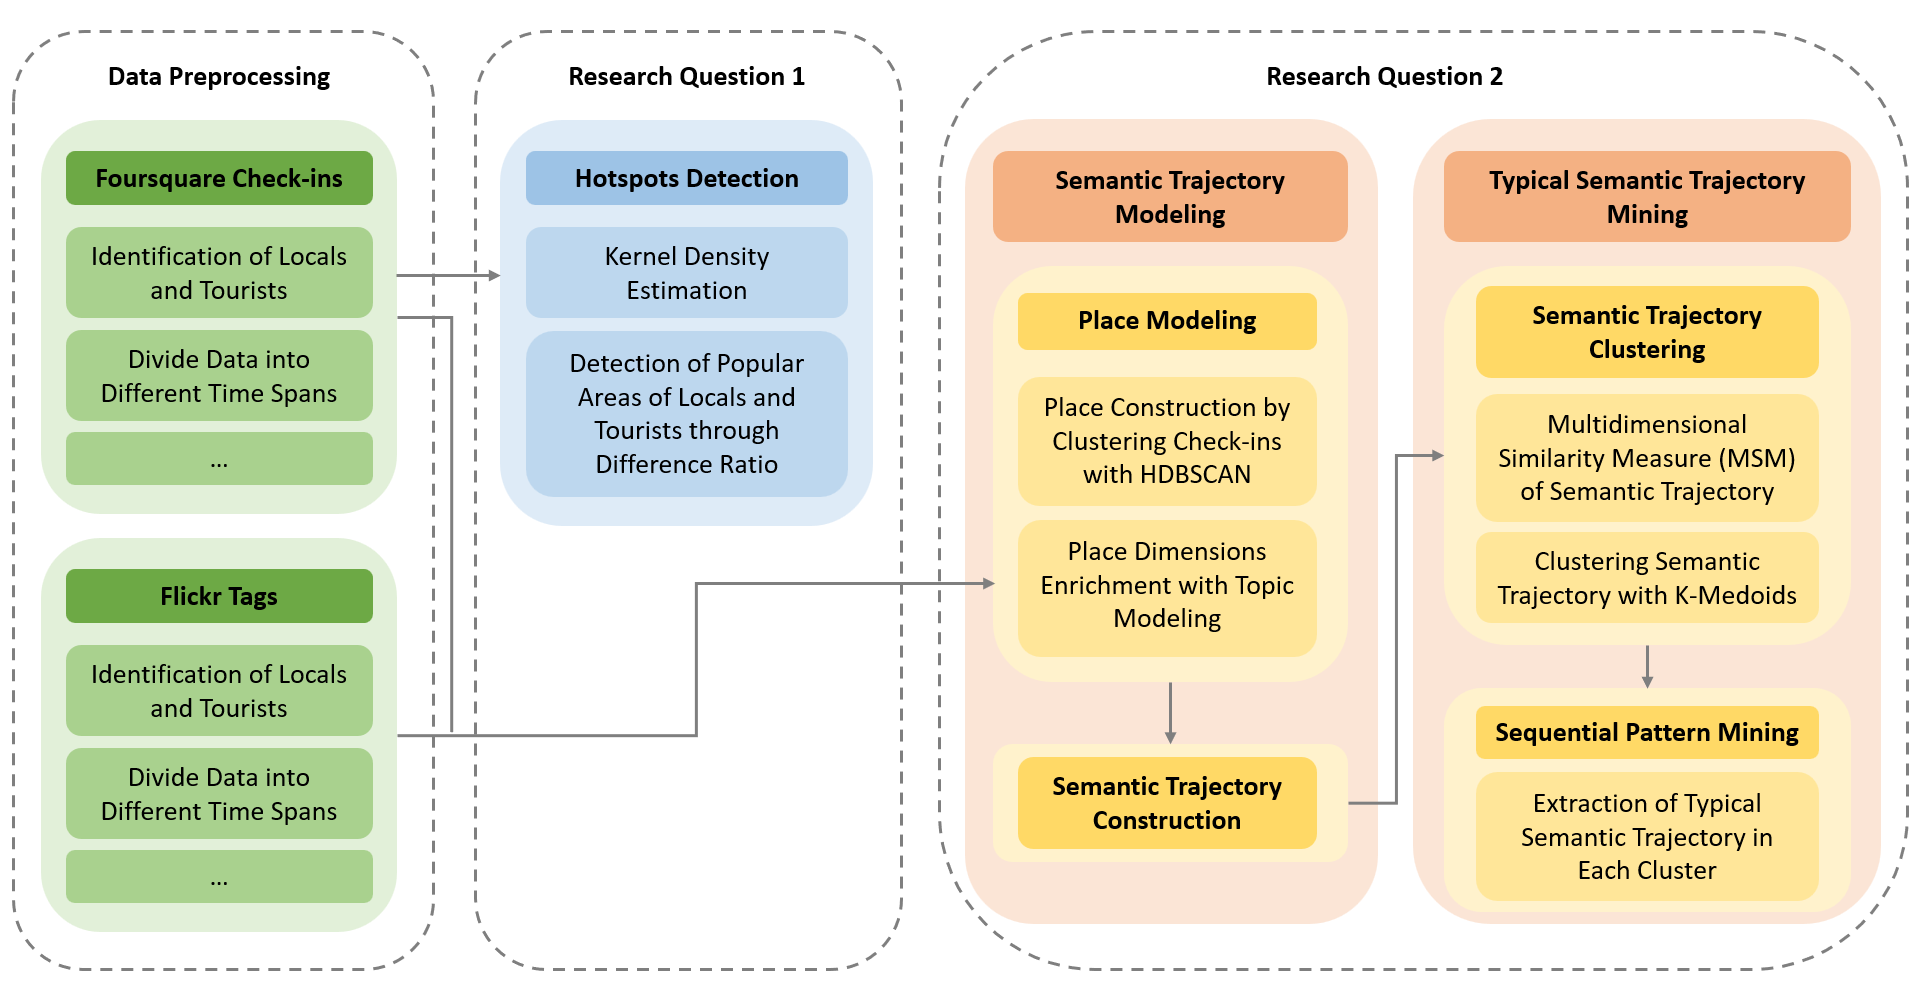
\includegraphics[width=1\textwidth]{figures/workflow.png}
\caption{\label{fig:workflow}Workflow.}
\end{figure}


\begin{figure}[h!]
\centering
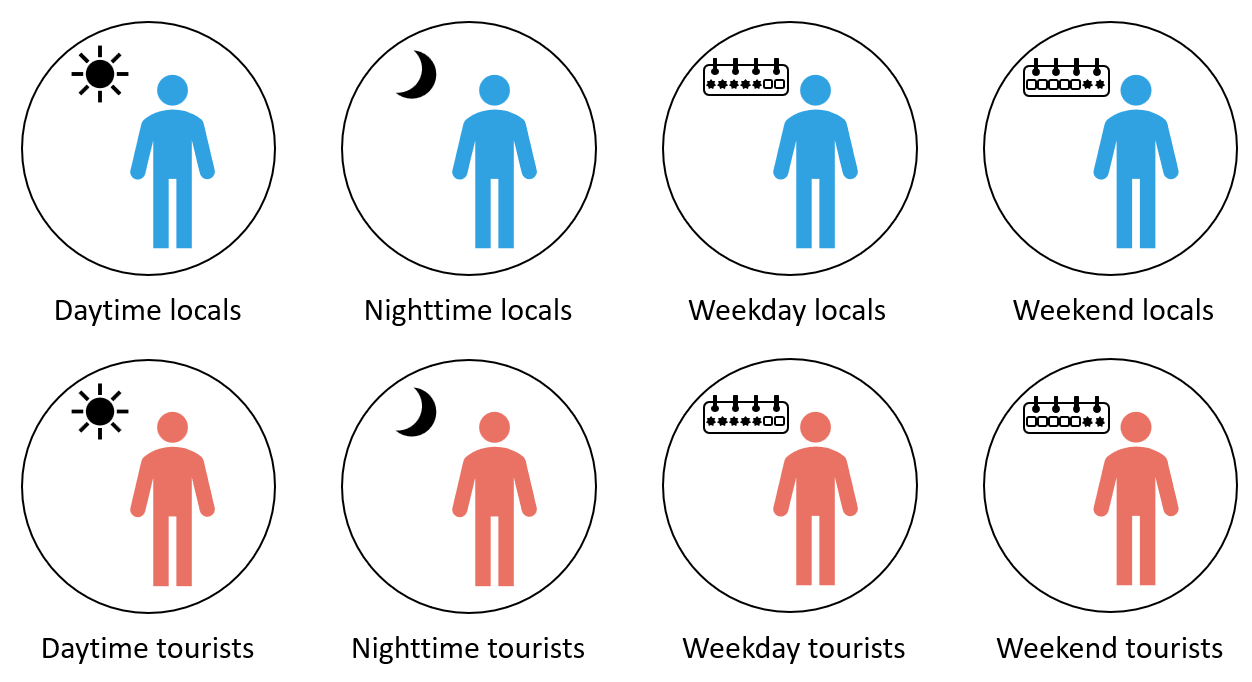
\includegraphics[width=0.8\textwidth]{figures/scene.png}
\caption{\label{fig:scene}Study scenes.}
\end{figure}

% ============================= || Hotspots Detection || =============================
\subsection{Hotspots Detection}\label{hotspots_detection}

% ====================== | Kernel Density Estimation | ======================
\subsubsection{Kernel Density Estimation}
Locals and tourists show distinct visiting preferences, which can be revealed through their distribution patterns. In this study, \acrfull{kde} was employed to identify visiting hotspots of these two groups based on the distribution of their check-ins. \acrshort{kde} estimates the probability density of data points with the kernel function, which helps to visualize the continuous distribution of discrete data points. Specifically, the estimated distribution is based on the distribution of existing data points in the neighborhood, and the more neighboring data points, the greater the estimated density is. To formally define \acrshort{kde}, consider a set of independent distributed random points, denoted as $x_{1}, x_{2}, ..., x_{n}$, the unknown density $f$ at any given point $x$ can be expressed as:

\begin{equation} \label{eq:kde}
\hat{f}_{h}(x) = \frac{1}{nh \sum_{i=1}^n k\bigg(\frac{x-x_i}{h}\bigg)}
\end{equation}

where $h$ is a bandwidth parameter that controls the degree of smoothing in \acrshort{kde}. Choosing an appropriate bandwidth is crucial as a large bandwidth may over-smooth the estimate, while a small bandwidth may under-smooth it, potentially hiding important features or introducing random noise. The kernel function $k$ is a smooth function to calculate the weighted average of neighboring observed data points. This weighting process effectively smooths out the data, with closer points receiving higher weights.

In this study, the seaborn.kdeplot function provided by the Python library seaborn \citep{waskom_seaborn_2021} was used to apply \acrshort{kde} to the Foursquare check-ins of locals and tourists and visualize the estimated distribution of these check-ins. The coordinates of the check-ins were converted to the EPSG:27700 projected coordinate system for the United Kingdom. The bandwidth method scott was applied to calculate the estimator bandwidth as the rule of scott allows fast computation for bandwidth selection. Additionally, the Gaussian kernel was used as the kernel smoother.

Since the distribution of check-ins of locals and tourists was assumed to differ across various time spans, this study applied \acrshort{kde} to visualize the distribution of check-ins for these two groups during the daytime and nighttime, as well as on weekdays and weekends. Visiting hotspots were determined based on the estimated density value in the output plot. By comparing the hotspots across different scenes (e.g., locals during the daytime, tourists on weekdays), along with the difference ratio discussed in the next section, this study aimed to explore which areas were more popular among locals and which areas were more popular among tourists.


% ====================== | Calculation of Difference Ratio | ======================
\subsubsection{Calculation of Difference Ratio}
Investigating the popularity of an area among locals and tourists can be achieved by examining the degree of their interaction within that area. In this study, the study area was rasterized, and the mixture degree of locals and tourists was investigated through raster analysis to identify popular areas among these two groups. The polygon of Greater London was divided into equal-sized rasters with a size of 1 km by 1 km. When assessing the mixture degree, both the number of visitors and the number of check-ins in each raster could be used, but the latter better reflected the activity density. To avoid bias caused by significant differences in the number of check-ins between locals and tourists within each raster, this study applied the difference ratio $R$, as previously utilized in a study by \cite{li_analyzing_2018}, to assess the mixture level between locals and tourists. The difference ratio is defined as:

\begin{equation} \label{eq:diff_ratio}
    R = \frac{t_{i}}{T}-\frac{l_{i}}{L}
\end{equation}

where $t_{i}$ represents the number of tourists' check-ins in the raster $i$, and $T$ represents the total number of tourists' check-ins shared citywide. Similarly, $l_{i}$ represents the number of locals' check-ins in the raster $i$, and $L$ represents the total number of locals' check-ins across the entire city. This ratio provides insights into the relative activity density between locals and tourists within each raster. A larger positive value of $R$ indicates a higher density of check-ins shared by tourists in that particular raster, while a larger negative value of \(R\) indicates a higher density of check-ins shared by locals in the raster.

Similar to the identification of hotspots using \acrshort{kde}, the mixture degree between locals and tourists was also calculated and visualized across various time spans. To facilitate comparison of the difference ratio across different scenes, the minimum and maximum values for the color mapping were set to -0.3 and 0.3, respectively, based on the extreme values of difference ratio across scenes. This ensured that all difference ratio values were colored within the same range. The colormap coolwarm was applied for visualization, with a deeper red color representing a larger positive value of difference ratio (indicating a higher proportion of tourists), and a deeper blue color representing a larger negative value of difference ratio (indicating a higher proportion of locals). The hotspots identified through \acrshort{kde} were further analyzed using the difference ratio to determine their popularity among locals or tourists.


% ============================= || Place Modeling || =============================
\subsection{Place Modeling} \label{place_modeling}

% ====================== | Place Construction | ======================
\subsubsection{Place Construction} \label{place_construction}

In this study, the concept of place refers to a part of geographical space that holds meaningful attributes, while check-in is a specific instance that represents an individual's interaction with a place. Figure~\ref{fig:place_construction_methodology} shows the process of place construction. Foursquare check-ins were clustered to build places using the \acrfull{hdbscan} \citep{campello_density-based_2013} algorithm. \acrshort{hdbscan} is a hierarchical extension of \acrshort{dbscan} that automatically determines the optimal number of clusters and can handle clusters of varying densities, which helps to reduce user input bias. Prior to clustering, a distance matrix among check-ins was computed and the features used for distance calculation included the coordinates and categories of check-ins. The Gower distance \citep{gower_general_1971} was used to construct the distance matrix as it could measure the dissimilarity between items with mixed numeric and categorical attributes. The coordinates of check-ins were standardized. And the check-in categories were converted into numerical values using label encoding and treated as categorical data in the distance measure. The importance of features was also considered, with coordinates weighted at 80\% and categories weighted at 20\%.

The hdbscan function provided by the Python library HDBSCAN \citep{mcinnes_hdbscan_2017} was used to cluster check-ins. A minimum of three check-ins within a cluster was set as the criterion for defining a place, ensuring that each place encompassed a certain number of check-ins. \acrshort{hdbscan} labeled check-ins with their corresponding clusters, while check-ins labeled as -1 were considered outliers and removed. To represent the boundary of a place, the convex hulls were constructed for the clusters of check-ins, creating polygons that approximated the areas covered by places. And the coordinate of the place was represented by the centroid of its convex hull, as shown in Figure~\ref{fig:place_construction_methodology}. It is important to note that check-ins of locals and tourists were differentiated across various time spans before constructing places, ensuring that each scene had its own distinct set of places.

To enrich the semantic information of places, three dimensions conceptualized by \cite{agnew_space_2011}, namely \textit{Location}, \textit{Locale}, and \textit{Sense of Place}, were annotated. The \textit{Location} dimension was represented by the borough name, specifically the borough where the majority of check-ins within a place cluster were located. The \textit{Locale} dimension was determined by the most frequently occurring check-in category within the place cluster. The \textit{Sense of Place} dimension utilized Flickr tags associated with the place cluster to capture people's perceptions. Topic modeling was applied to generate a set of topics based on these tags, providing a representation of the \textit{Sense of Place}. The process of topic modeling is introduced in the next section. With these three dimensions annotated, places in different scenes were compared across different scenes based on their distributions and the frequency of the three dimensions.

\begin{figure} [!h]
\centering
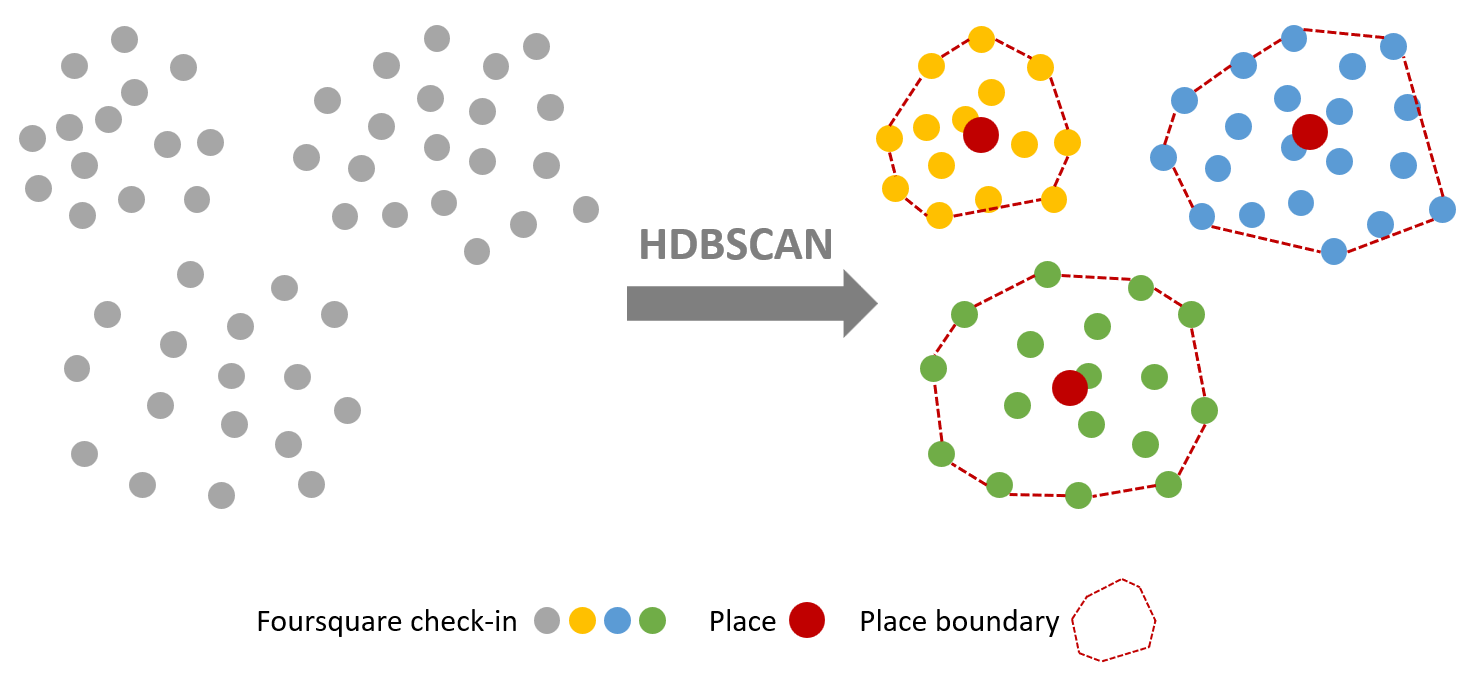
\includegraphics[width=0.8\textwidth]{figures/place_construction_methodology.png}
\caption{\label{fig:place_construction_methodology}Place construction.}
\end{figure}

% ====================== | Topic Modeling | ======================
\subsubsection{Topic Modeling}

This study applied \acrfull{lda}, a topic modeling technique, to generate topics describing places based on Flickr tags, and the process is illustrated in Figure~\ref{fig:topic_modeling_methodology}. \acrshort{lda} discovers underlying topics from a large collection of words. In this study, after the preprocessing steps outlined in Section \ref{preprocess_flickr}, the Flickr tags within each place were gathered as words to form a \textit{document}, with each \textit{document} comprising the Flickr tags for a specific place. The input to the \acrshort{lda} model is a \textit{corpus} consisting of \textit{documents}. The \textit{corpus} is a matrix with the size of $word \times document$. Each row of this matrix stores the frequency of words in each document, denoted as a vector $w = {w_{1}, w_{2}, ..., w_{v}}$. $v$ is the number of words in the \textit{vocabulary} (all distinct words in a corpus), and $w_{v}$ denotes the frequency of word $v$ in the document. It is important to note that Flickr tags were also separated based on two groups of people in different time spans, thus the corpus in every scene was unique.

The \acrshort{lda} model generated a set of topics as its primary output, along with topic distribution and topic terms, facilitating the determination and interpretation of topics for each place. The topic distribution for each place consisted of a list of topics and the corresponding probabilities of the place belonging to each topic. The topic terms for each topic comprised a list of tags, accompanied by their probabilities of association with that topic. In this study, each place was assigned the most probable topic, and the interpretation of topics relied on the corresponding tags and probabilities. This study implemented the \acrshort{lda} model using the gensim.models.wrappers.LdaMallet function provided by the Python library gensim \citep{rehurek_software_2010}.

The semantic quality of the generated topics is sensitive to the number of topics. If too many topics are generated, some topics might become similar to each other, making it difficult to interpret topics. The \acrshort{lda} model requires users to determine the number of topics as input, thus it is crucial to choose appropriate topic numbers. The \textit{coherence value} was employed to measure the semantic quality of topics. This value was calculated based on the co-occurrence probability of words within a topic, specifically within the place clusters assigned to that topic. The \textit{coherence value} can be defined as:

\begin{equation} \label{eq:coherence_value}
    coherence = \sum_{i}\sum_{j<1}\log\frac{D(w_{j},w_{i})+\beta}{D(w_{i})}
\end{equation}

where $\beta$ is to prevent log zero errors. $D(w_{j},w_{i})$ represents the number of co-occurrence of two words in a document, and $D(w_{i})$ is the number of occurrences of the more probable words. A higher coherence value indicates that the words within a topic are closely related to each other and the topic is more interpretable to humans.

In cases where certain places had no tags within their convex hulls, a topic imputation was employed to assign topics to those empty places. This imputation relied on the topic distribution of nearby places that did contain Flickr tags in a weighted average approach. The imputed topic distribution represented the probability distribution across a predefined set of topics. Based on this imputed topic distribution, the places were assigned the most probable topics. The calculation for imputed topic distribution of the target empty place can be expressed as:

\begin{equation} \label{eq:topic_imputation}
    P_{imputed} = \frac{1}{W}\sum_{i}{n}w_{i}P_{i}
\end{equation}

where $P_{i}$ represents the topic distribution for place $i$, and $n$ is the number of places in the neighborhood of the target empty place. The weight assigned to each place $w_{i}$ is determined by the distance between place $i$ and the target empty place, and it is defined as:

\begin{equation} \label{eq:topic_imputation_w_i}
    w_{i} = \exp(\frac{-d(i,j)^2}{2\sigma^2})
\end{equation}

where $\sigma$ controls the smoothness of the weighting function. $d(i,j)$ is the distance between place $i$ and place $j$. A larger value of $\sigma$ gives more weight to places that are closer to the target empty place, while a smaller value of $\sigma$ gives more weight to places that are farther away. This study set $\sigma$ as 500 for topic imputation in all scenes. $W$ ensures that the sum of the weights to 1 so that the imputed topic distribution is a valid probability distribution, and it is defined as:

\begin{equation} \label{eq:topic_imputation_W}
    W = \sum_{i}^{n}w_{i}
\end{equation}

\begin{figure} [!h]
\centering
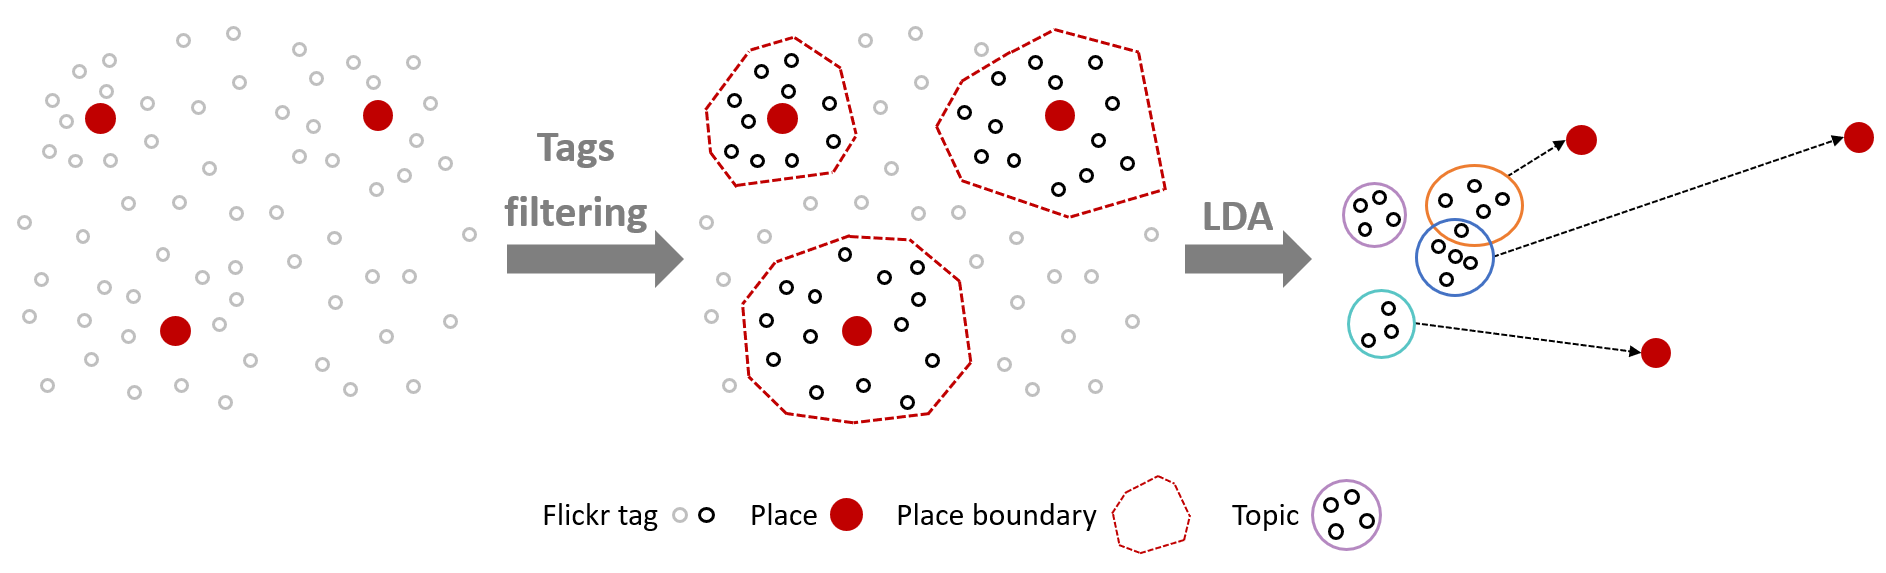
\includegraphics[width=0.9\textwidth]{figures/topic_modeling_methodology.png}
\caption{\label{fig:topic_modeling_methodology}Tags filtering and topic modeling.}
\end{figure}

% ============================= || Typical Semantic Trajectory Mining || =============================
\subsection{Typical Semantic Trajectory Mining} \label{typical_semantic_trajectory_mining}

% ====================== | Semantic Trajectory Construction | ======================
\subsubsection{Semantic Trajectory Construction}
This study aimed to compare city perceptions under different scenes by analyzing semantic trajectories. Semantic trajectories were constructed based on the places defined in Section \ref{place_construction}. The semantic trajectories can be defined as a sequence of places $T = \langle p_{1}, p_{2}, ..., p_{n} \rangle$, with $p = (x,y,D_{p})$ being the place $i$ at the position $(x,y)$ annotated by the three dimensions of the place $D_{p}$, including \textit{Location}, \textit{Locale}, and \textit{Sense of Place}.

By connecting places in a visiting order, it becomes possible to track individuals' movements. However, within one's movement, there might be multiple trajectories. Hence, it is necessary to determine the beginning and end of each trajectory, as illustrated in Figure~\ref{fig:trajectory_begin_end}. In this study, a time gap of five hours served as a criterion to determine whether two consecutive places belonged to the same trajectory. Specifically, if the time gap between two consecutive places exceeded five hours, the former place was considered the last position of the current trajectory, while the latter place marked the beginning of the new trajectory. Moreover, the analysis of city perception focused on long trajectories as they conveyed more information. Therefore, only trajectories consisting of more than five places were considered in this study.

\begin{figure} [!h]
\centering
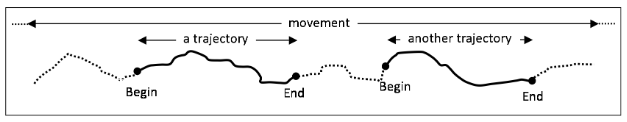
\includegraphics[width=0.75\textwidth]{figures/begin_end.png}
\caption{\label{fig:trajectory_begin_end}Trajectories extracted from a movement track \citep{parent_semantic_2013}.}
\end{figure}


% ====================== | Semantic Trajectory Similarity Measure | ======================
\subsubsection{Semantic Trajectory Similarity Measure} \label{traj_similarity}
Before clustering semantic trajectories, it is essential to measure their similarity. Existing methods often focus on the spatial or spatiotemporal aspects of raw trajectories, neglecting the multiple dimensions present in semantic trajectories. To address this, the \acrfull{msm} proposed by \cite{furtado_multidimensional_2016} was employed in this study to construct the similarity matrix for semantic trajectories. 

\acrshort{msm} is a similarity measure for multidimensional sequences, considering the similarity across all dimensions. In two semantic trajectories denoted as $T_{1}$ and $T_{2}$, the general term for each dimension $D_{k}$ ($k = 1, 2, 3, 4$) represents the following: $D_{1}$ represents the spatial position of the semantic trajectory, while $D_{2}$, $D_{3}$, and $D_{4}$ correspond to the three semantic dimensions: \textit{Location}, \textit{Locale}, and \textit{Sense of Place}. The distance between two places, $p_{1} \in T_{1}$ and $p_{2} \in T_{2}$, is computed using the distance function $dist_{k}(p_{1},p_{2})$. Additionally, a maximum distance threshold $maxDist_{k}$ is set for each dimension to determine whether a pair of places $(p_{1},p_{2})$ can be considered a match in $D_{k}$.

The similarity score was calculated by considering each dimension separately, and the scores in all four dimensions were summed up. Each dimension was assumed to have different importance, represented by the weight $w_{k}$ assigned to the corresponding dimension $D_{k}$. It is important to note that the sum of the weights of all dimensions should be equal to 1. In this study, the weights were set as follows: $w_{1}=0.4$, $w_{2}=0.1$, $w_{3}=0.3$, $w_{4}=0.2$. $D_{1}$ (spatial distance) was assumed to be more important in the similarity measure for trajectories, thus it weighted 0.4. $D_{2}$ (\textit{Location}) weighted only 0.1 as it was represented by borough names in the space, which was correlated with $D_{1}$. $D_{3}$ (\textit{Locale}) and $D_{4}$ (\textit{Sense of Place}) weighted 0.5 in total so that the non-spatial dimensions could also be equally considered. The similarity score between the two places $p_{1}$ and $p_{2}$ is defined as the sum of the weighted match scores across all dimensions, as represented in the following equation:

\begin{equation} \label{eq:match_score}
    score(p_{1},p_{2}) = \sum_{k=1}^{4}(match_{k}(p_{1},p_{2})w_{k})
\end{equation}

where $match_{k}(p_{1},p_{2})$ determines whether the places are matched or not based on the max distance threshold $maxDist_{k}$, and it is defined in Equation~\ref{eq:match}. In this study, to handle the different data types of dimensions, each dimension was assigned a specific distance function and a threshold to determine whether $p_{1}$ and $p_{2}$ were matched. For the spatial position dimension $D_{1}$, the Euclidean distance was applied, as defined in Equation~\ref{eq:dist_euclidean}, where $x$ and $y$ represent the coordinates of places. A maximum distance threshold $maxDist_{1}$ of 1 km was set, meaning that if the distance between $p_{1}$ and $p_{2}$ exceeded 1 km, the match score of these two points was 0. For the semantic dimensions $D_{2}$, $D_{3}$, and $D_{4}$, which were categorical data, the discrete distance was applied, as shown in Equation~\ref{eq:dist_discrete}. In this case, the distance can only be either 0 or 1, thus a maximum distance threshold of 0.5 was set for $maxDist_{2}$, $maxDist_{3}$, and $maxDist_{4}$.

\begin{equation} \label{eq:match}
    match_{k}(p_{1},p_{2}) = \begin{cases}
    1 & \text{if } dist_{k}(p_{1},p_{2}) \leq maxDist_{k}  \\
    0 & \text{otherwise}
    \end{cases}
\end{equation}

\begin{equation} \label{eq:dist_euclidean}
    dist_{euclidean}(p_{1},p_{2}) = \sqrt{(p_{1}.x-p_{2}.x)^2+(p_{1}.y-p_{2}.y)^2}
\end{equation}

\begin{equation} \label{eq:dist_discrete}
    dist_{discrete}(p_{1},p_{2}) = \begin{cases}
    0 & \text{if } p_{1}.type = p_{2}.type  \\
    1 & \text{otherwise}
    \end{cases}
\end{equation}

Since a place $p_{1} \in T_{1}$ can be matched with multiple places in $T_{2}$, the objective of \acrshort{msm} is to find the best matching score for each place $p_{1}$ with $T_{2}$. The parity of $T_{1}$ with $T_{2}$, denoted as $parity(T_{1},T_{2})$, is defined as the sum of the highest score of all places $p_{1} \in T_{1}$ with $T_{2}$, and the equation is:

\begin{equation} \label{eq:parity}
    parity(T_{1},T_{2}) = \sum_{p_{1}\in T_{1}}\max\{score(p_{1},p_{2}) : p_{2} \in T_{2}\}
\end{equation}

Finally, the multidimensional similarity measure $MSM(T_{1},T_{2})$ is calculated by averaging the parity of $T_{1}$ with $T_{2}$ and the parity of $T_{2}$ with $T_{1}$, as defined as:

\begin{equation} \label{eq:msm}
    MSM(T_{1},T_{2}) = \begin{cases}
    0 & \text{if } |T_{1}| = 0 \text{ or } |T_{2}| = 0 \\
    \frac{parity(T_{1},T_{2}) + parity(T_{2},T_{1})}{|T_{1}|+|T_{2}|} & \text{otherwise}
    \end{cases}
\end{equation}

In this study, the Python library trajminer developed by \cite{petry_trajminer_2019} was applied to construct the similarity matrix for semantic trajectories. Specifically, the trajminer.similarity.MSM function was used, with the distance functions, thresholds, and weights specified. Overall, by employing the \acrshort{msm}, this study considered the multiple dimensions of semantic trajectories and computed a similarity matrix that captured the matching scores and weights for each dimension, providing a comprehensive assessment of trajectory similarity.


% ====================== | Semantic Trajectory Clustering | ======================
\subsubsection{Semantic Trajectory Clustering}
The K-medoids algorithm was employed to cluster semantic trajectories. The term K-medoids was introduced by \cite{kaufman_partitioning_1990} with their Partitioning Around Medoids (PAM) algorithm. K-medoids is a classical clustering technique that divides the dataset of $n$ objects into $k (k<n)$ clusters, with the number of clusters $k$ predefined. Similar to K-means, K-medoids aims to minimize the distance between data points and the center point within a cluster. The reason for applying K-medoids to cluster trajectories is that it selects existing points as the centers of the clusters, resulting in more interpretable cluster centers and increased robustness to outliers.

In the K-medoids algorithm, the dissimilarity between trajectories needs to be measured. In this study, the dissimilarity was precomputed based on the trajectory similarity described in Section \ref{traj_similarity}. The trajectory dissimilarity between each pair of trajectories is defined as:

\begin{equation} \label{eq:dissimilarity}
    dissimilarity(T_{1},T_{2}) = 1-MSM(T_{1},T_{2})
\end{equation}

To perform the clustering for semantic trajectories, the trajminer.clustering.KMedoids function from the Python library trajminer was employed. With the precomputed dissimilarity matrix, the initial cluster medoids were determined using the approach introduced by \cite{park_simple_2009}. This approach iteratively updates the medoids and assigns trajectories to each cluster until the sum of distances from all trajectories to their medoids reaches the minimum.

The K-medoids algorithm also requires users to define the number of clusters as input. In this study, the optimal number of clusters was determined based on the silhouette score and the intracluster distance. The silhouette score measures the similarity of a trajectory to its own cluster compared to other clusters. The score ranges from -1 to 1, with a score closer to 1 indicating a well-matched trajectory within its own cluster and a poor match to neighboring clusters. The intracluster distance is the average distance between trajectories within a cluster and measures the compactness of the cluster. A larger intracluster distance indicates that the trajectories within the same cluster are less similar.

After clustering all semantic trajectories, an exploratory data analysis was conducted to investigate the distribution of trajectories and the frequency of three semantic dimensions within each cluster. This analysis aimed to uncover the unique characteristics of these clusters, providing additional insights into the investigation of city perception through semantic trajectories.

% ====================== | Sequential Pattern Mining | ======================
\subsubsection{Sequential Pattern Mining}
While the trajectories selected as the cluster centers by the K-medoids algorithm can serve as representatives of their clusters, it is beneficial to identify typical semantic trajectories within each cluster to enhance the interpretation of clustering results. In this study, the \acrfull{prefixspan} algorithm \citep{pei_mining_2004}, a sequential pattern mining technique, was applied to detect frequently visited sequences under different scenes. The fundamental concept of \acrshort{prefixspan} is to recursively project the sequence databases into smaller projected databases based on current sequential patterns. It utilizes a user-defined support threshold to mine sequential patterns by identifying frequent subsequences in a sequence database. The support represents the number of occurrences of the subsequence in the database, and subsequences with support above the specified threshold are extracted as the sequential patterns of interest.

For the sequential pattern mining process, the Python library prefixspan \footnote{\url{https://pypi.org/project/prefixspan/}} was utilized in this study. The semantic trajectories within each cluster were treated as the sequence database for the mining process. Considering the number of trajectories at different time spans, the minimum support was set in a range from 2 to 5 to ensure that the typical trajectories could be mined. The output for each trajectory cluster consisted of several sets of frequently visited places in sequential order, along with their corresponding support values.

The study of city perceptions in different scenes involved analyzing the typical semantic trajectories extracted from each cluster. A comparison of the distribution of these trajectories was made to explore the different areas visited by locals and tourists across different time spans. The first two semantic dimensions \textit{Location} and \textit{Locale} were utilized to examine the visiting purposes of these popular trajectories. Additionally, the third semantic dimension \textit{Sense of Place} was applied to capture people's descriptions along these trajectories.

\clearpage

% ============================================ ||| Results ||| ============================================
\section{Results}
This chapter presents the results of this study. The spatiotemporal patterns of hotspots are displayed in Section \ref{patterns_hotspots} to investigate the popular areas among locals and tourists across various time spans (RQ1). Section \ref{patterns_places} shows the distribution of places as these places are the fundamental elements in the construction of semantic trajectories. The distribution of semantic trajectories and the city perception along these trajectories across various time spans are presented in Section \ref{patterns_traj} to answer RQ2.

% ============================= || Spatiotemporal Patterns of Hotspots || =============================
\subsection{Spatiotemporal Patterns of Hotspots} \label{patterns_hotspots}

To investigate the popularity of different areas among locals and tourists at various times, Foursquare check-ins were utilized to detect spatiotemporal hotspots. Figure~\ref{fig:foursquare_checkins_count} reveals the number and temporal pattern of check-ins. Locals are more active than tourists, generating a greater number of check-ins throughout different periods. Notably, daytime check-ins outnumber nighttime check-ins. Figure~\ref{fig:foursquare_checkins_trend} shows the temporal pattern of check-ins. Locals display three prominent spikes in the number of check-ins during the daytime, specifically at 8 am, 12 pm, and 6 pm. Conversely, their activities diminish during the nighttime, particularly at midnight. On the other hand, tourists are more active at 12 pm but show reduced activity levels after 6 pm. Furthermore, weekdays experience a higher number of check-ins compared to weekends. Locals exhibit a consistent sharing pattern from Monday to Thursday, with a notable spike on Fridays, and when it comes to weekends, locals share significantly fewer check-ins. Tourists display a similar pattern from Monday to Thursday but exhibit increased activities on Fridays and Saturdays, followed by fewer check-ins on Sundays.


\begin{figure}[!h]
\centering
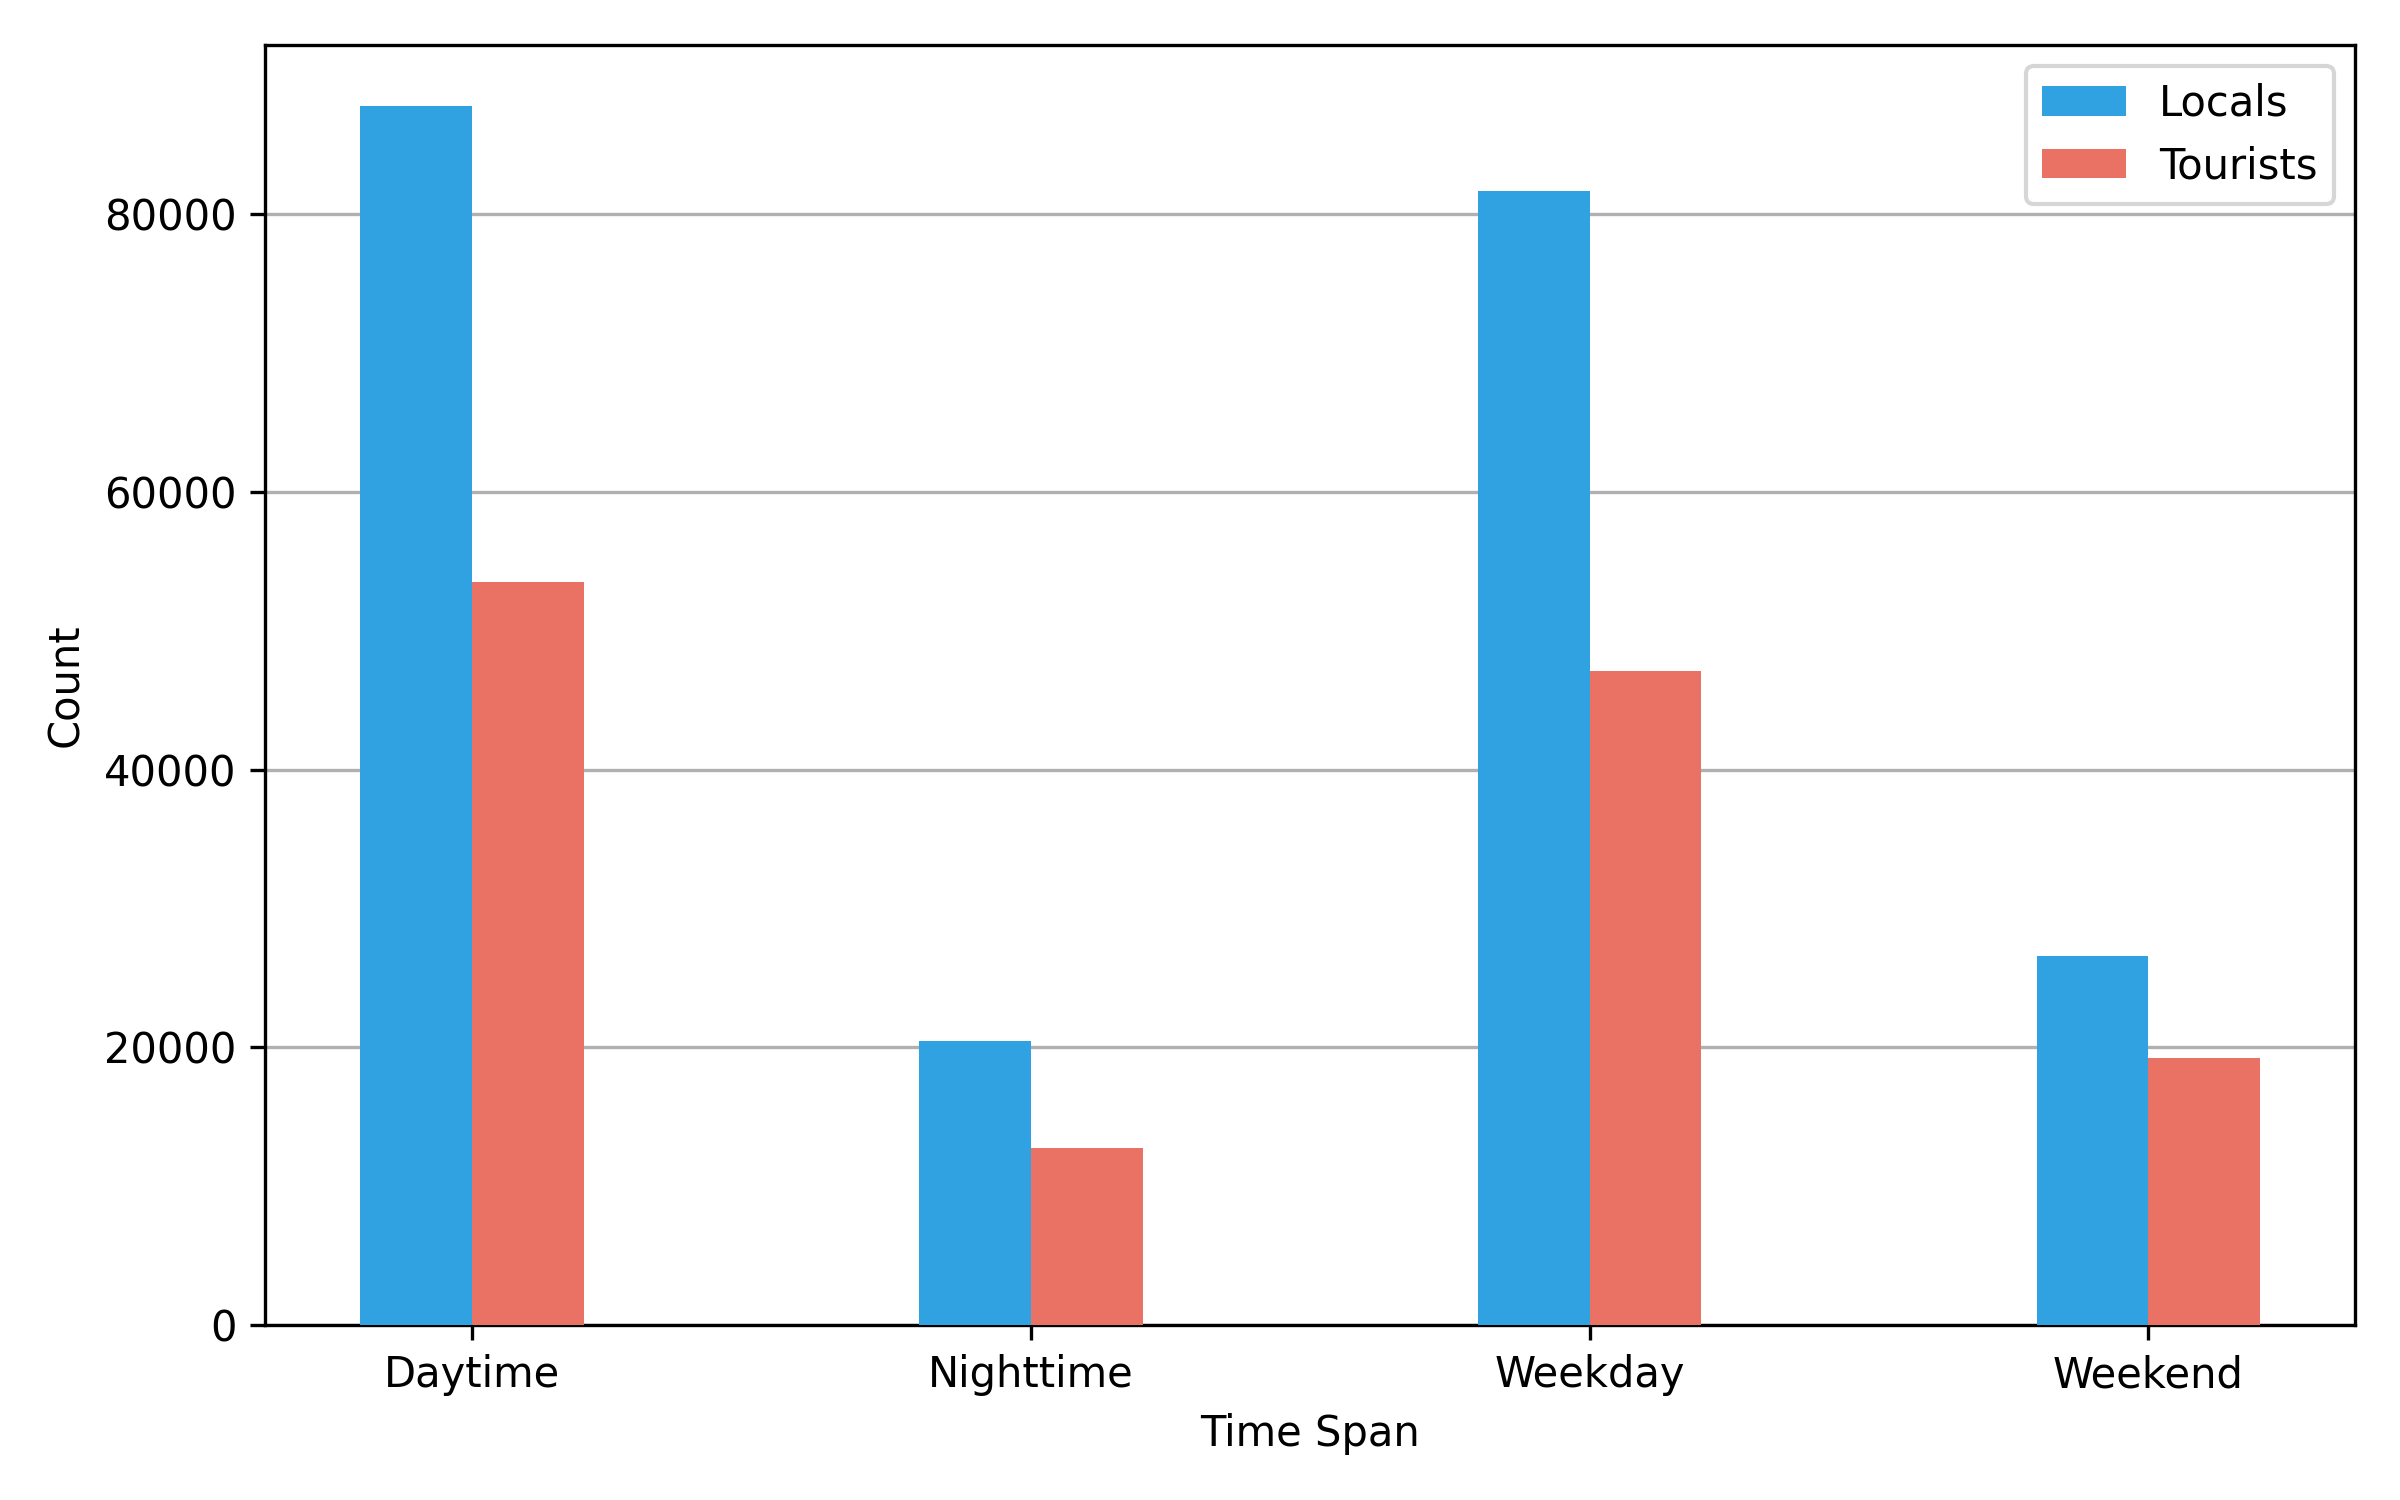
\includegraphics[width=0.75\textwidth]{figures/foursquare_checkins_count.png}
\caption{\label{fig:foursquare_checkins_count}Number of Foursquare check-ins of locals and tourists across time spans.}
\end{figure}

\begin{figure}[!h]

\begin{subfigure}{0.5\textwidth}
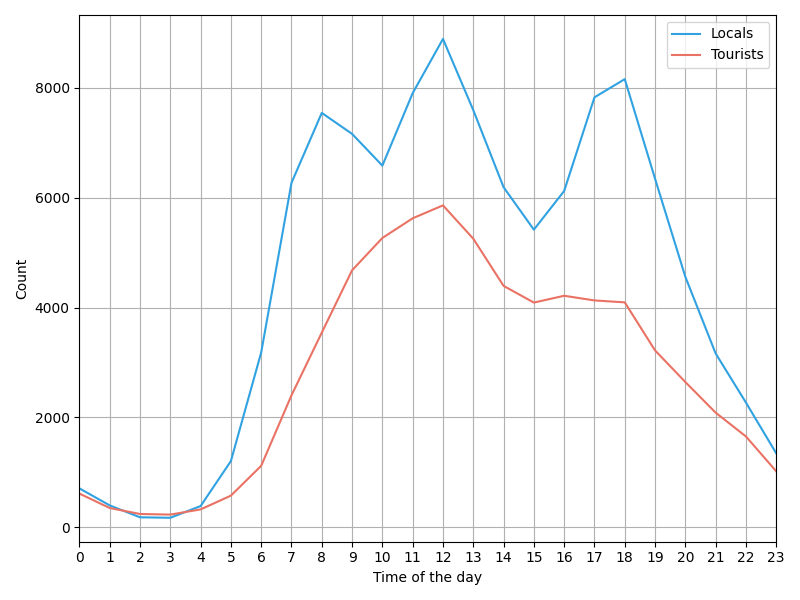
\includegraphics[width=1\linewidth]{figures/foursquare_trend_day.png} 
\caption{Day pattern.}
\label{fig:kde_locals_weekday}
\end{subfigure}
\begin{subfigure}{0.5\textwidth}
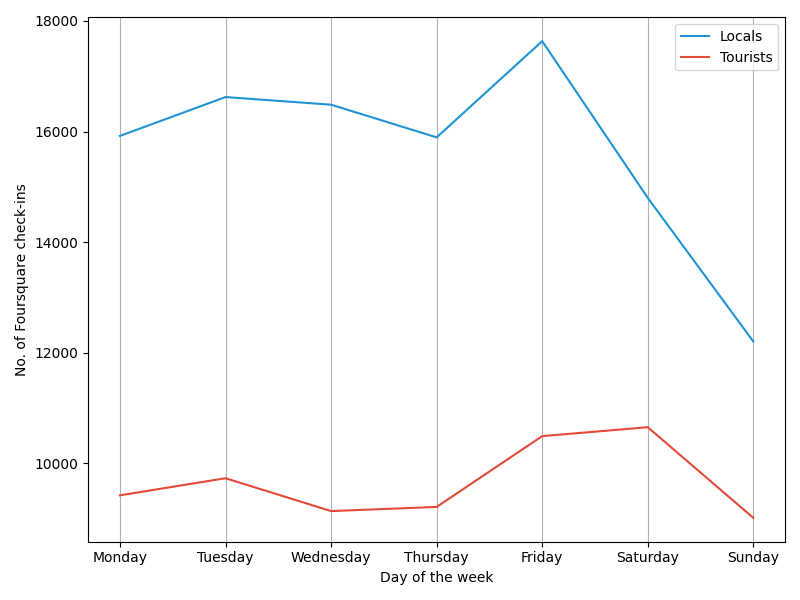
\includegraphics[width=1\linewidth]{figures/foursquare_trend_week.png}
\caption{Week pattern.}
\label{fig:kde_tourists_weekday}
\end{subfigure}

\caption{Temporal pattern of Foursquare check-ins.} \label{fig:foursquare_checkins_trend}
\end{figure}


% ====================== | Hotspots of Locals and Tourists | ======================
\subsubsection{Hotspots of Locals and Tourists} \label{hotspots}

% ============== Daytime vs. Nighttime ==============
\subsubsubsection{Daytime vs. Nighttime}
% daytime
The estimated distribution of Foursquare check-ins during the daytime is displayed in Figure~\ref{fig:kde_daytime}. Locals exhibit a similar hotspot distribution pattern with tourists but share fewer check-ins across London. The primary hotspots of locals and tourists are located in the city center, specifically Westminster, Camden, and the City of London. These boroughs contain an abundance of cultural and historical landmarks with high transportation connectivity, leading to a substantial influx of people. Another notable hotspot is situated around Stratford in Newham, where the Stratford Shopping Centre is located, appealing to individuals who enjoy shopping. Additionally, the southern region of Hillingdon, where Heathrow Airport is located, is another hotspot where people share a large number of check-ins. Furthermore, the boundary of Richmond upon Thames and Kingston upon Thames reveals an aggregation of check-ins, and these boroughs contain thriving communities with history and natural beauty. One notable difference between locals and tourists is the presence of work-related hotspots for locals. The City of London is found to be attractive to locals as this area serves as a major business hub, with numerous corporate headquarters providing employment opportunities. Similarly, Canary Wharf, located near the Isle of Dogs within Tower Hamlets, represents another hotspot for locals due to its status as part of London's central business district. Moreover, boroughs located on the outskirts of London, such as Croydon, Merton, Bromley, Brent, and Harrow, form smaller yet noteworthy hotspots. These areas are characterized by their residential settlement and exhibit a greater concentration of locals compared to tourists.


\begin{figure}[!h]

\begin{subfigure}{0.5\textwidth}
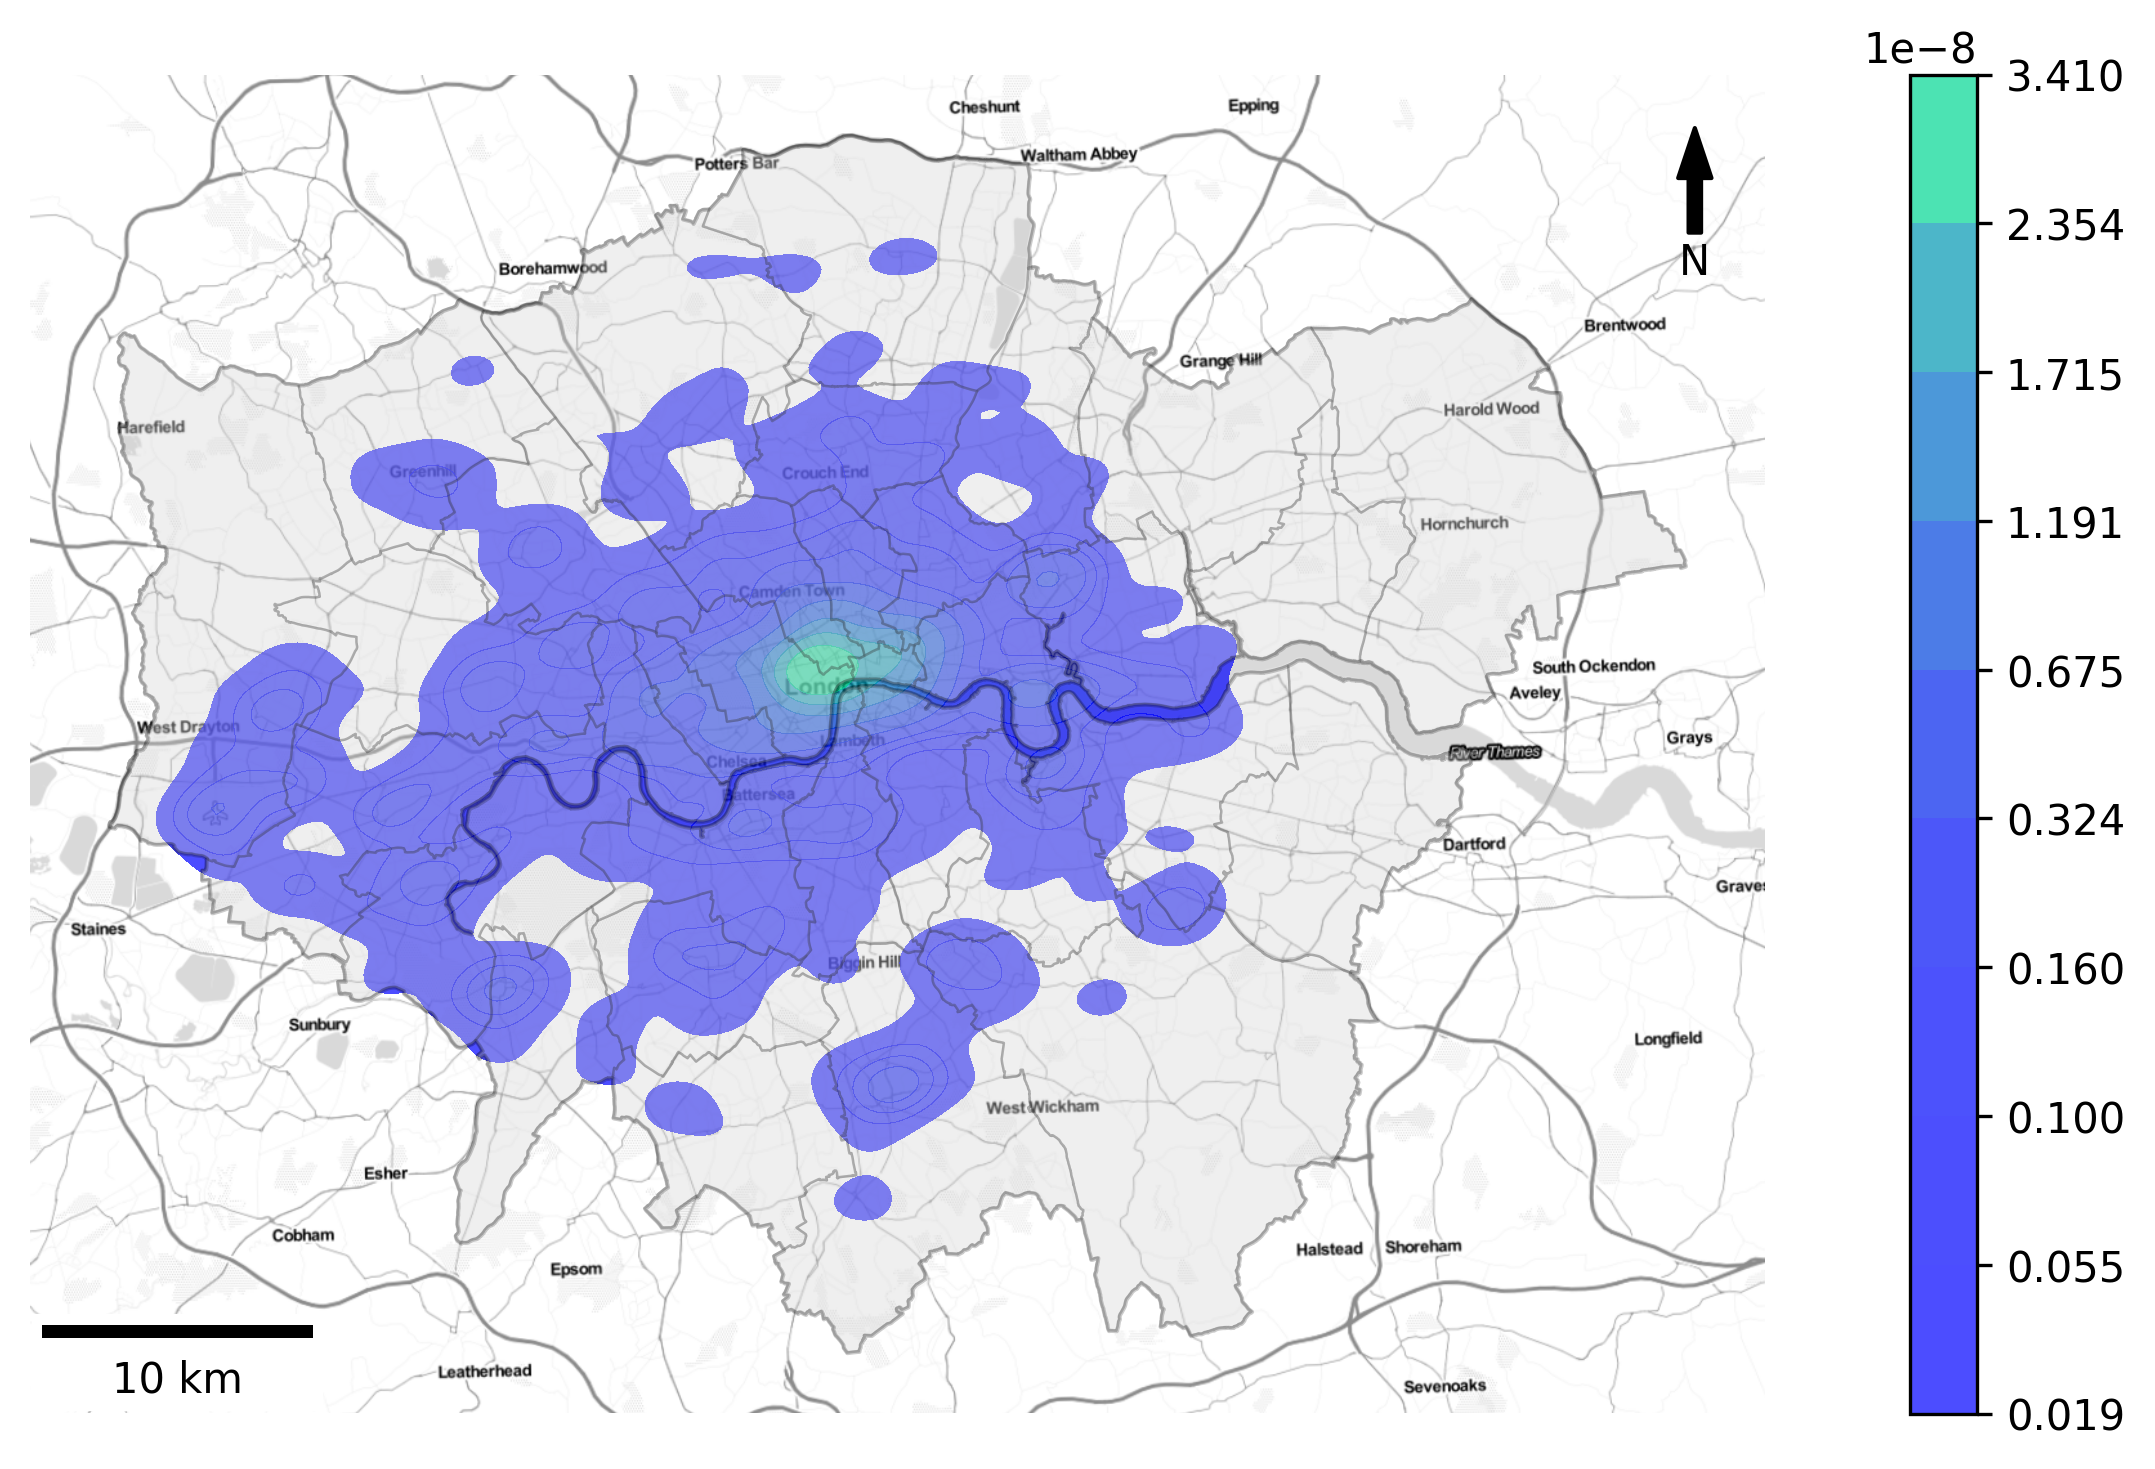
\includegraphics[width=1\linewidth]{figures/kde_locals_daytime.png} 
\caption{Locals.}
\label{fig:kde_locals_daytime}
\end{subfigure}
\begin{subfigure}{0.5\textwidth}
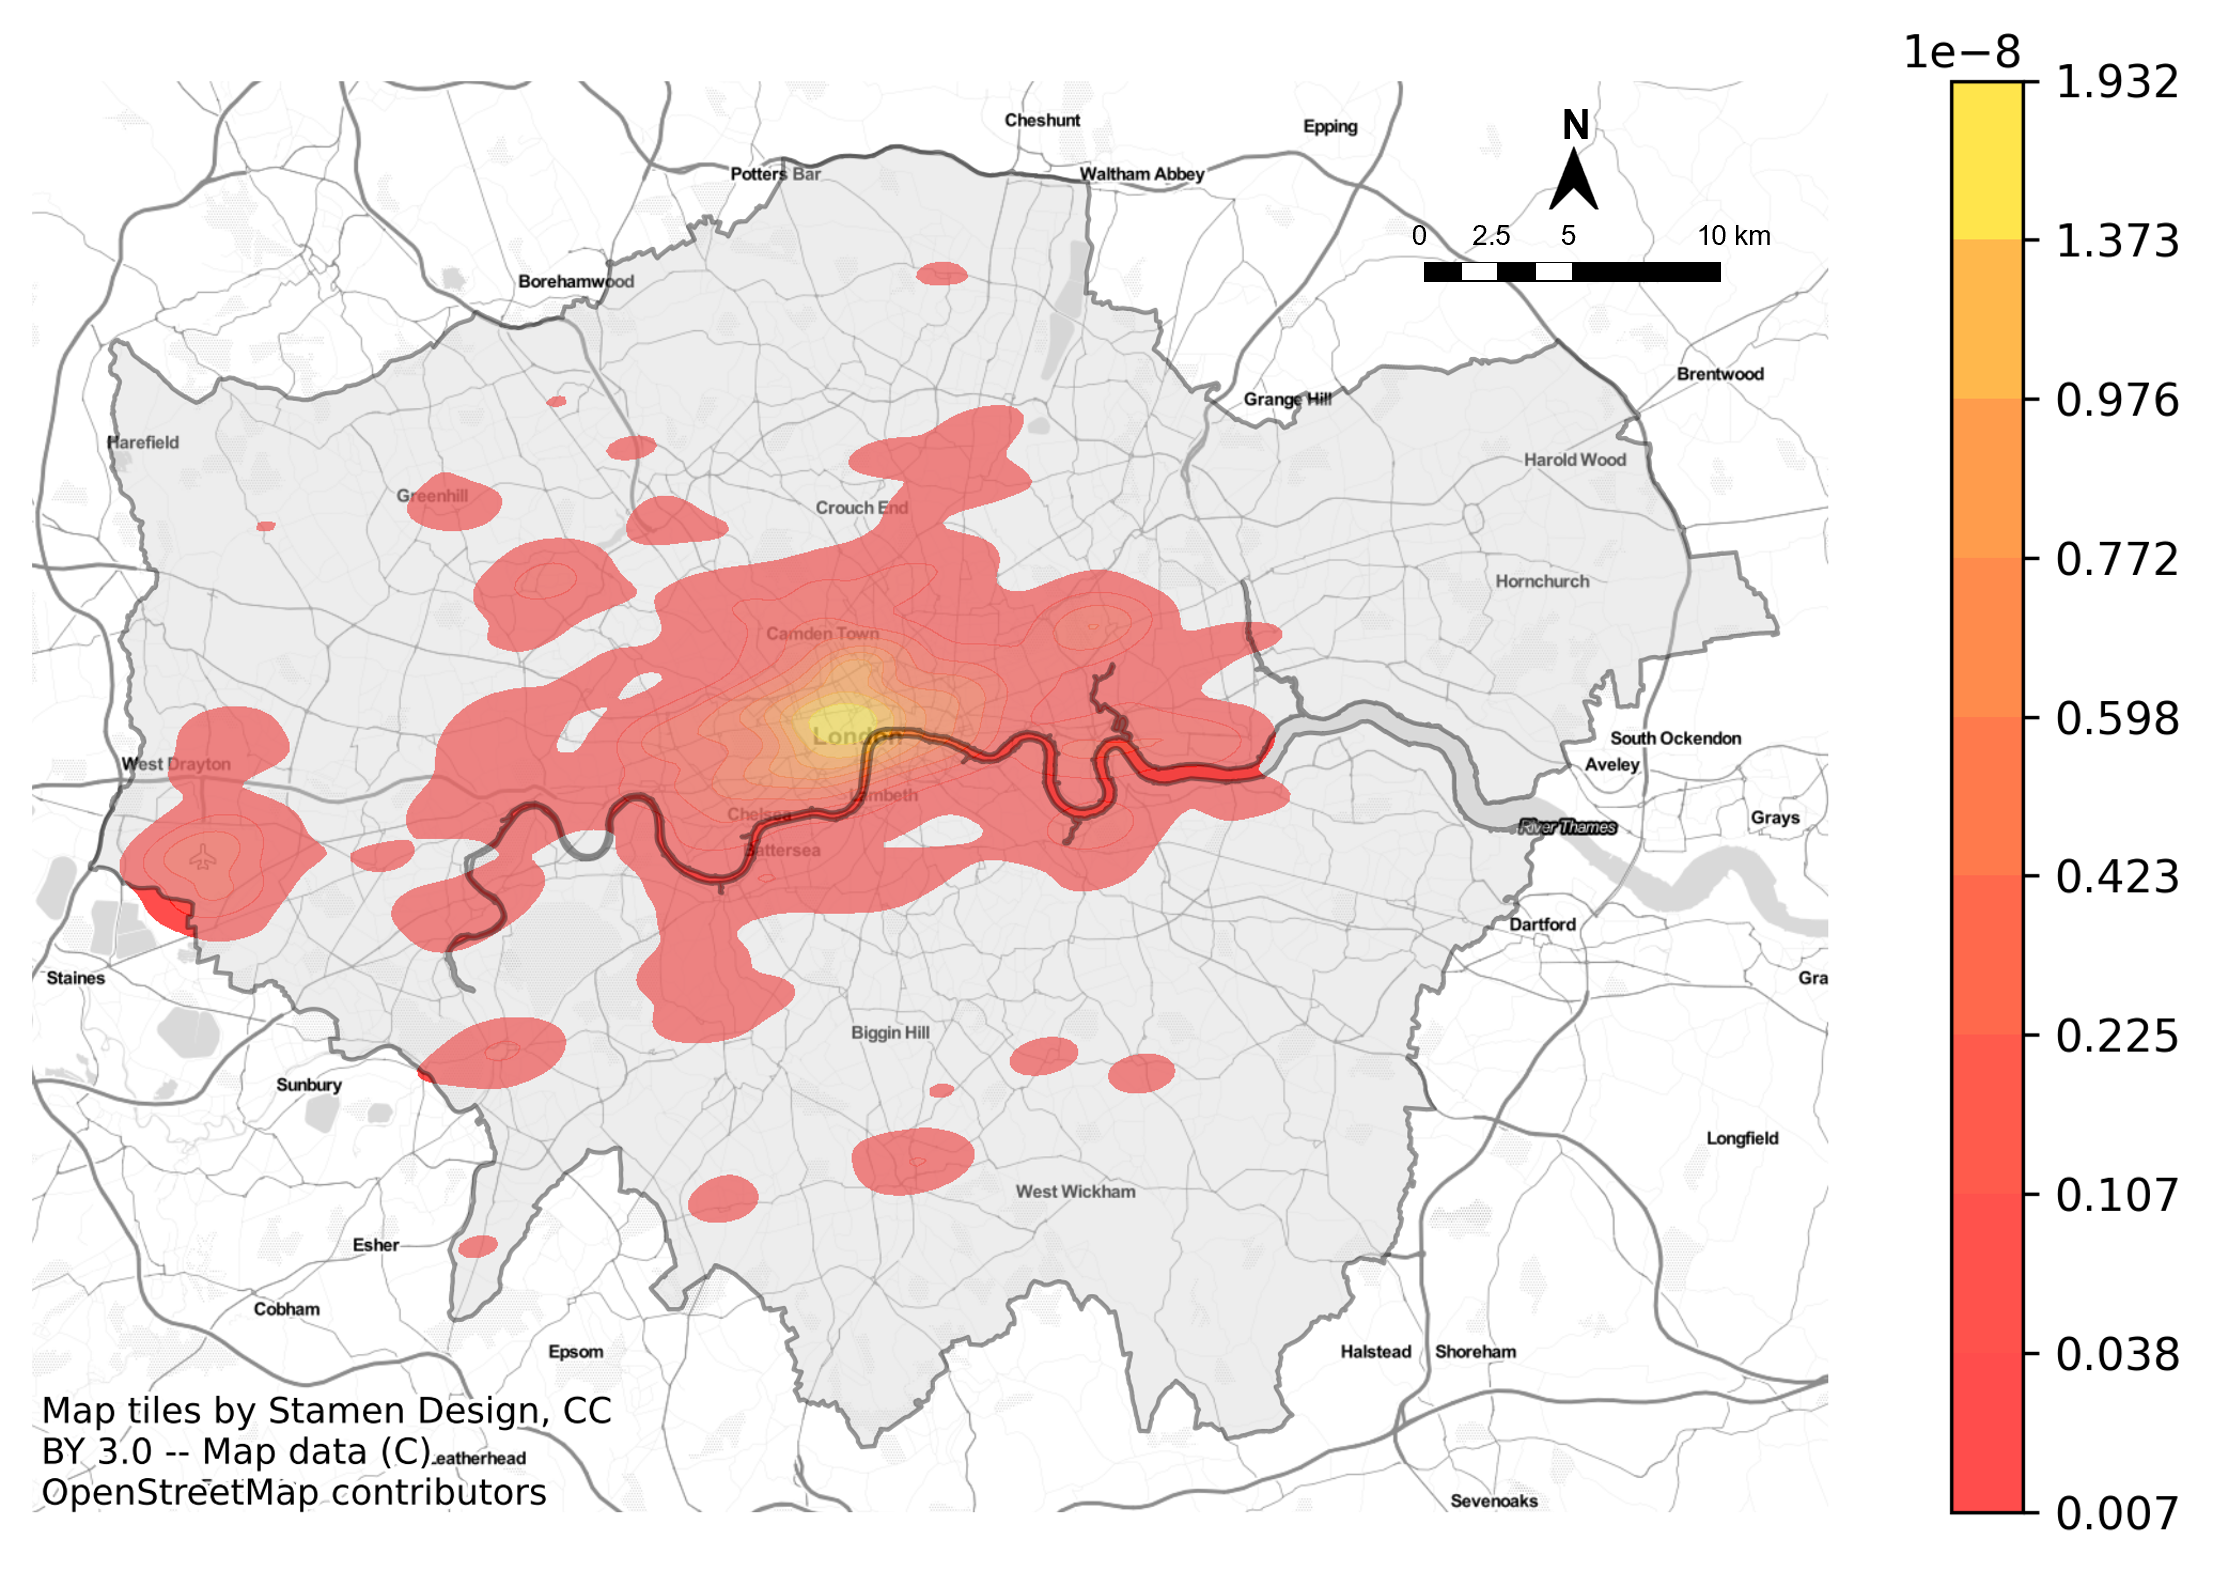
\includegraphics[width=1\linewidth]{figures/kde_tourists_daytime.png}
\caption{Tourists.}
\label{fig:kde_tourists_daytime}
\end{subfigure}

\caption{Kernel density estimation of Foursquare check-ins during the daytime.} \label{fig:kde_daytime}
\end{figure}

% nighttime & comparison
When it comes to the nighttime, the city center remains the primary hotspot for both locals and tourists. However, locals become less active compared to the daytime, with a decreased concentration of check-ins, while tourists keep similar activity levels (Figure~\ref{fig:kde_nighttime}). In addition to its cultural and historical attractions, the city center is also a renowned area that offers abundant shopping and entertainment options. For instance, Oxford Street and Regent Street in central London provide vibrant nightlife scenes. For locals, the concentration of check-ins in the city center during the nighttime is lower compared to the daytime. Furthermore, the hotspot around Canary Wharf, a bustling business district, diminishes, which indicates a reduced number of locals visiting this area during the nighttime. However, the hotspots around Heathrow Airport and outskirts boroughs, such as Croydon, Bromley, and Harrow, remain prominent. This suggests that these areas are aggregated with a significant number of locals, possibly due to air transport activities ad residential settlements. In terms of tourists, although the primary hotspot remains in the city center, the concentration of check-ins in this area decreases during the nighttime. Moreover, there is a reduction or disappearance of hotspots in the outer part of London except for the area around Heathrow Airport, indicating a decrease in the number of tourists visiting these settlement regions during the nighttime.


\begin{figure}[!h]

\begin{subfigure}{0.5\textwidth}
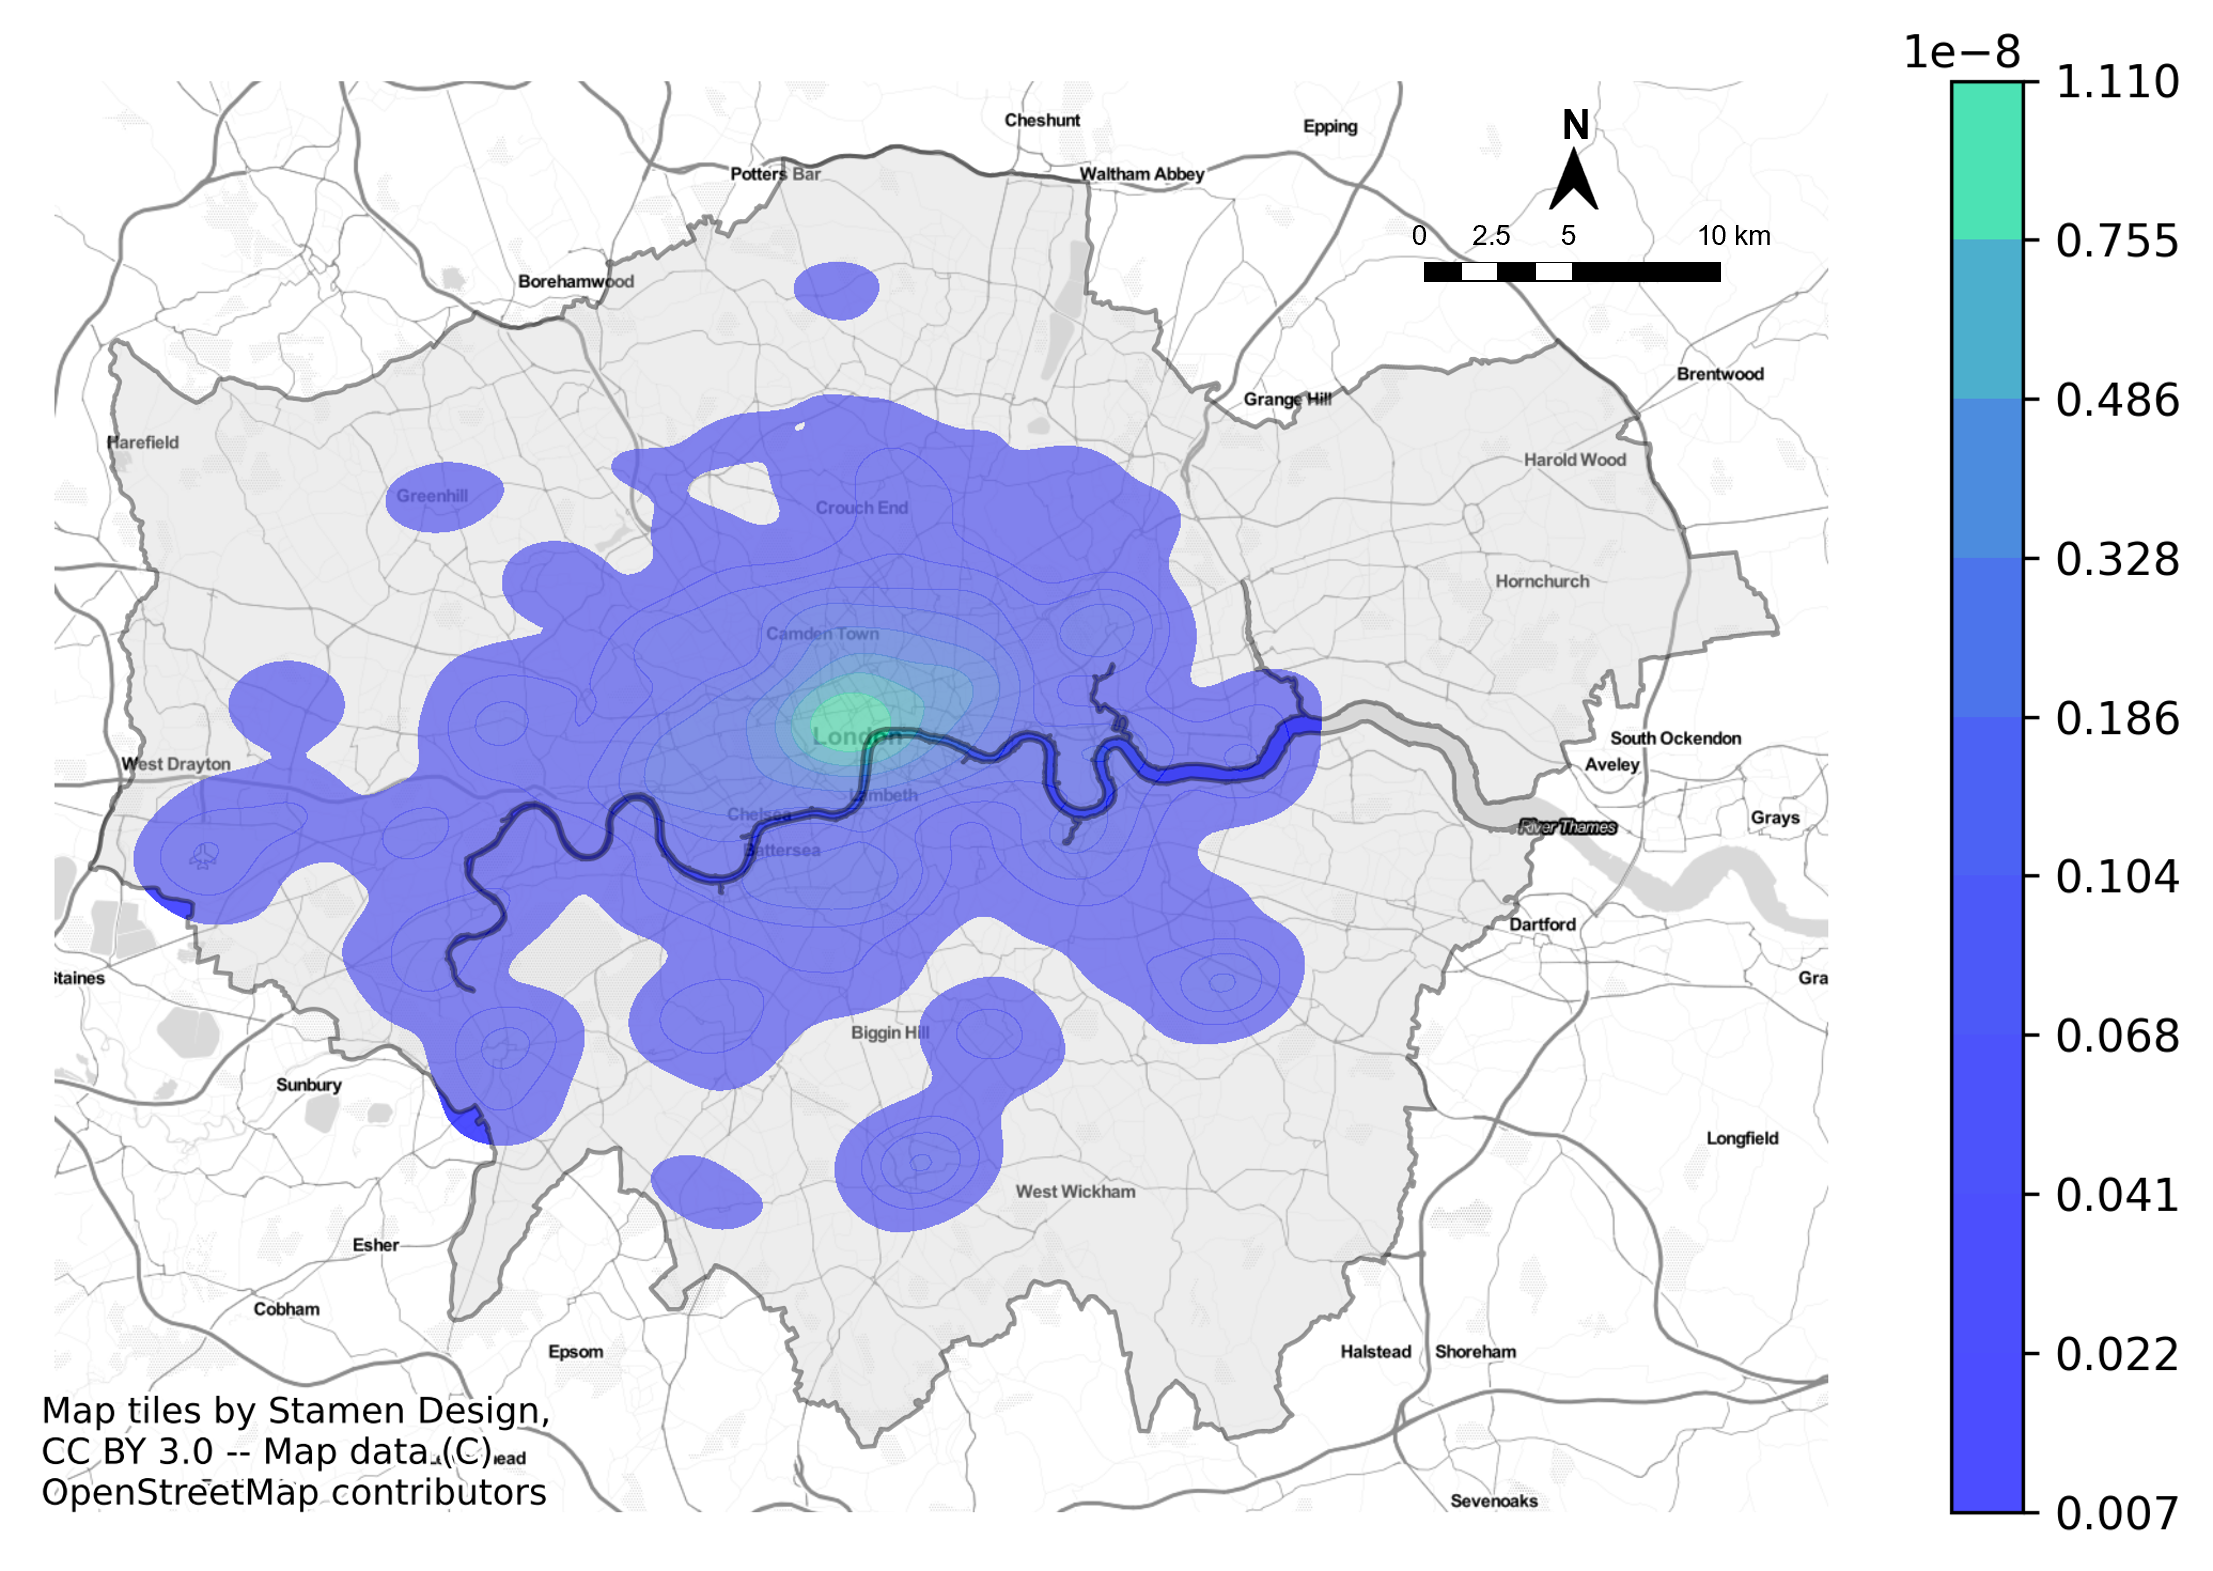
\includegraphics[width=1\linewidth]{figures/kde_locals_nighttime.png} 
\caption{Locals.}
\label{fig:kde_locals_nighttime}
\end{subfigure}
\begin{subfigure}{0.5\textwidth}
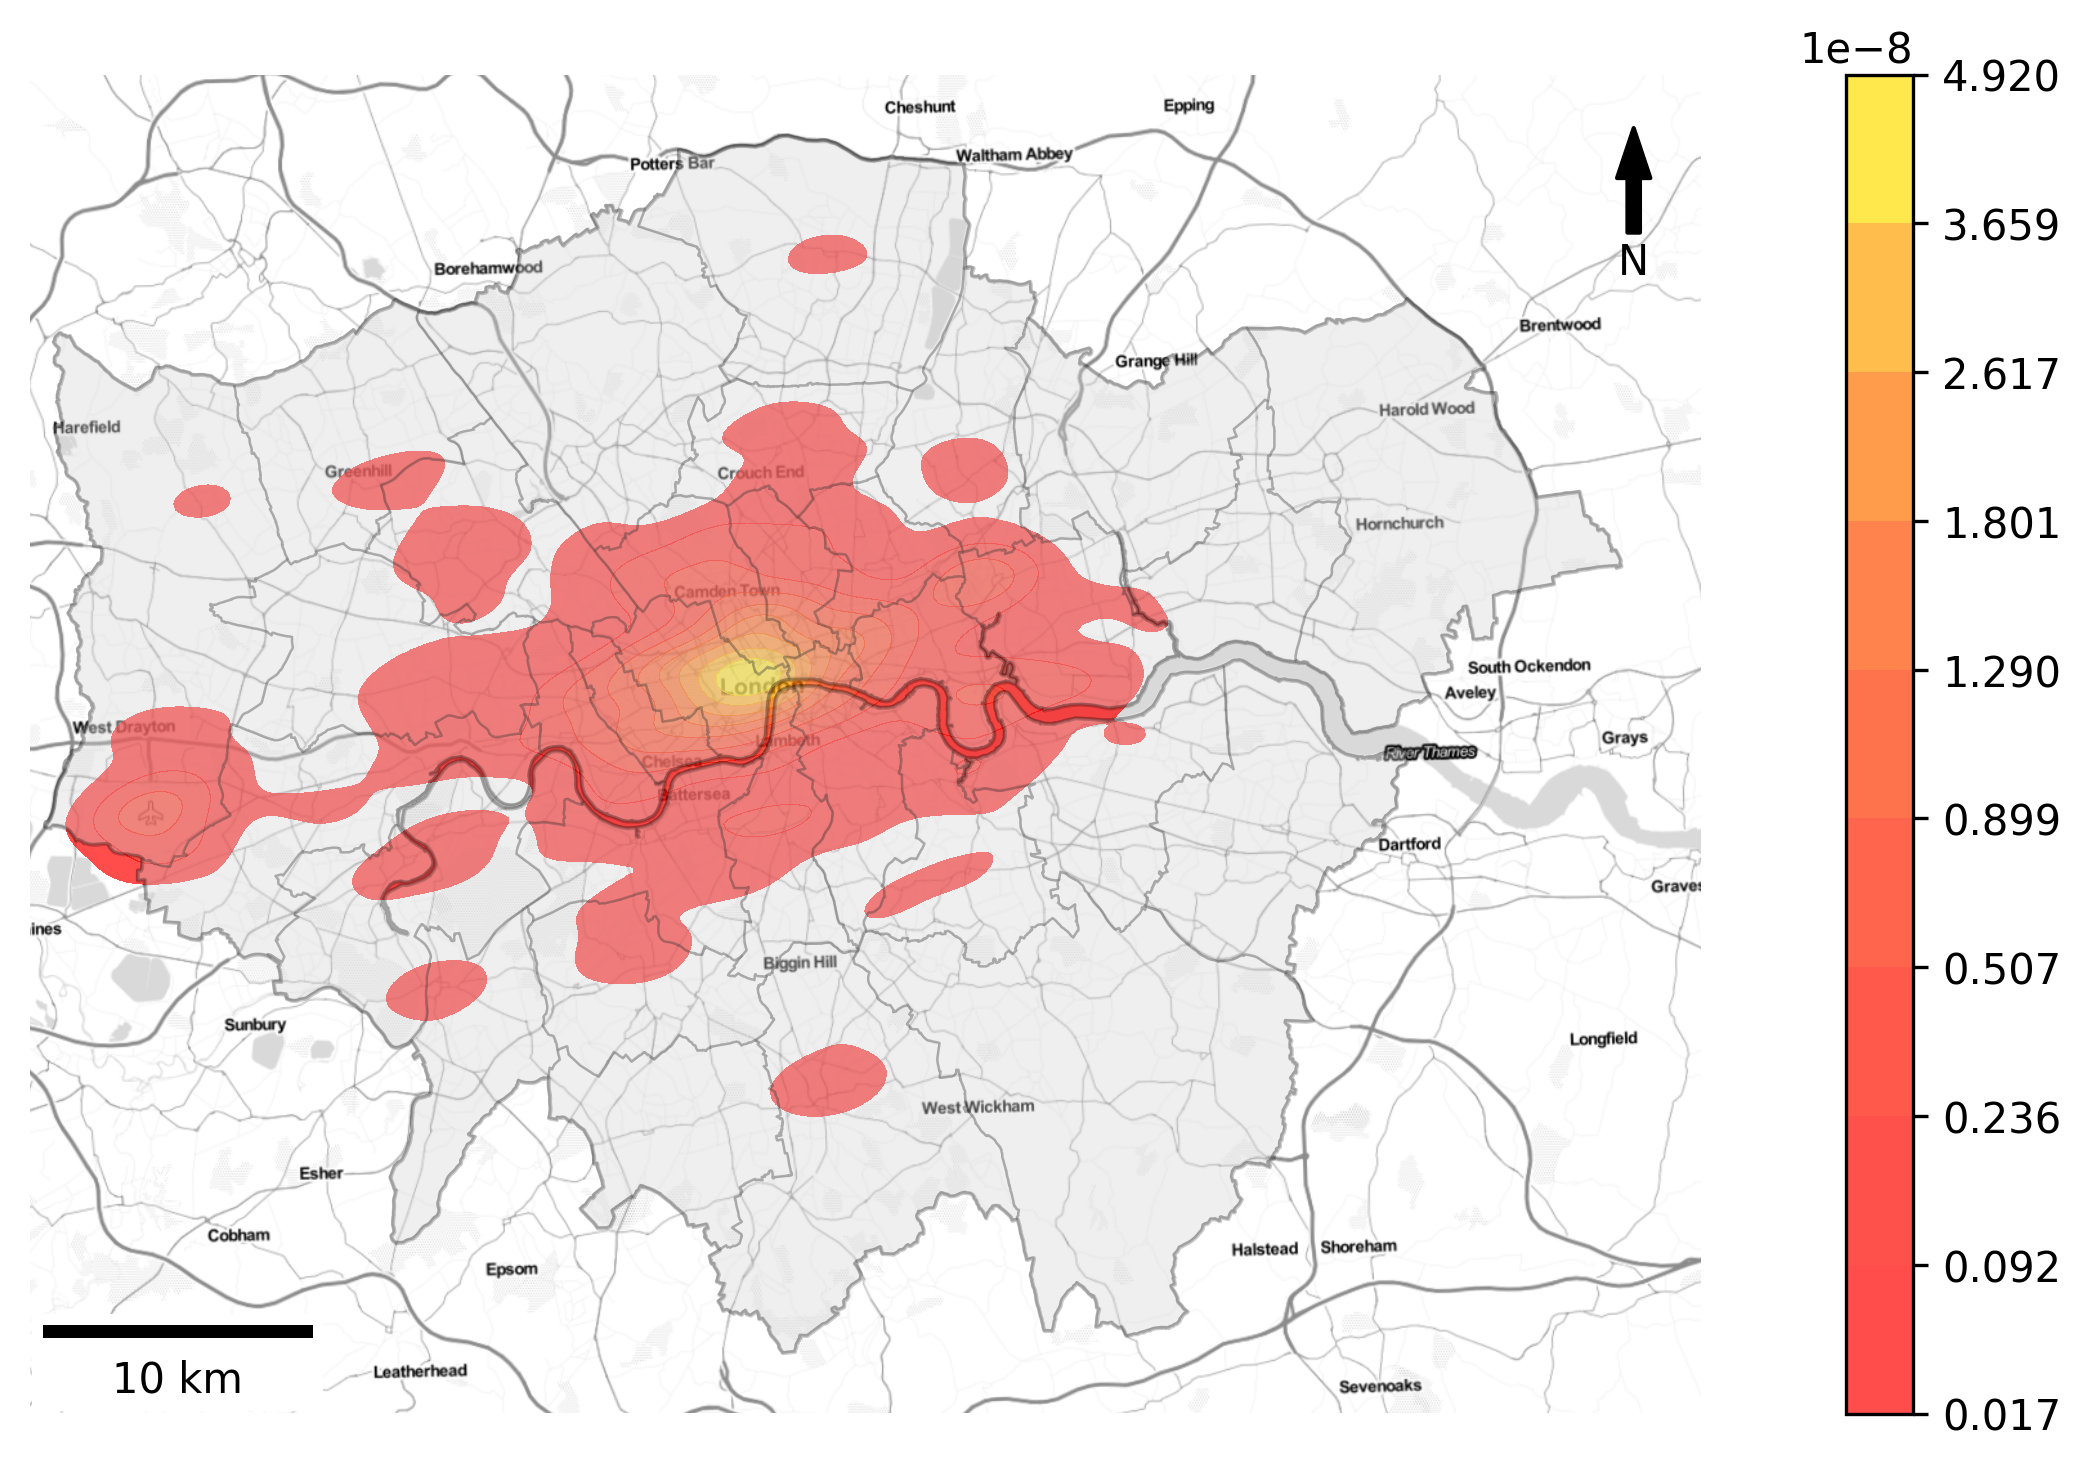
\includegraphics[width=1\linewidth]{figures/kde_tourists_nighttime.png}
\caption{Tourists.}
\label{fig:kde_tourists_nighttime}
\end{subfigure}

\caption{Kernel density estimation of Foursquare check-ins during the nighttime.} \label{fig:kde_nighttime}
\end{figure}


% ============== Weekday vs. Weekend ==============
\subsubsubsection{Weekday vs. Weekend}
% weekday
Figure~\ref{fig:kde_weekday} displays the estimated distribution of check-ins shared by locals and tourists on weekdays. Locals exhibit a relatively lower concentration of check-ins across London compared to tourists. Though both locals and tourists have their primary hotspots in the city center, the distributions of their hotspots are different. The primary hotspot of locals is close to the City of London and Canary Wharf, as these regions serve as important business districts for weekday work engagements. Consistent with the hotspot distribution observed during the daytime, locals also visit the outskirts of London, such as Heathrow Airport in Hillingdon, as well as settlement regions in Croydon, Merton, Harrow, etc. In contrast, the primary hotspot of tourists in the city center gravitates towards the vicinity of Westminster and Camden on weekdays. These areas contain numerous tourist attractions and shopping destinations, appealing to lots of tourists. The outer part of London is less popular among tourists, but it is noteworthy that Hillingdon, where Heathrow Airport is located, gains more popularity among tourists compared to other areas.


\begin{figure}[!h]

\begin{subfigure}{0.5\textwidth}
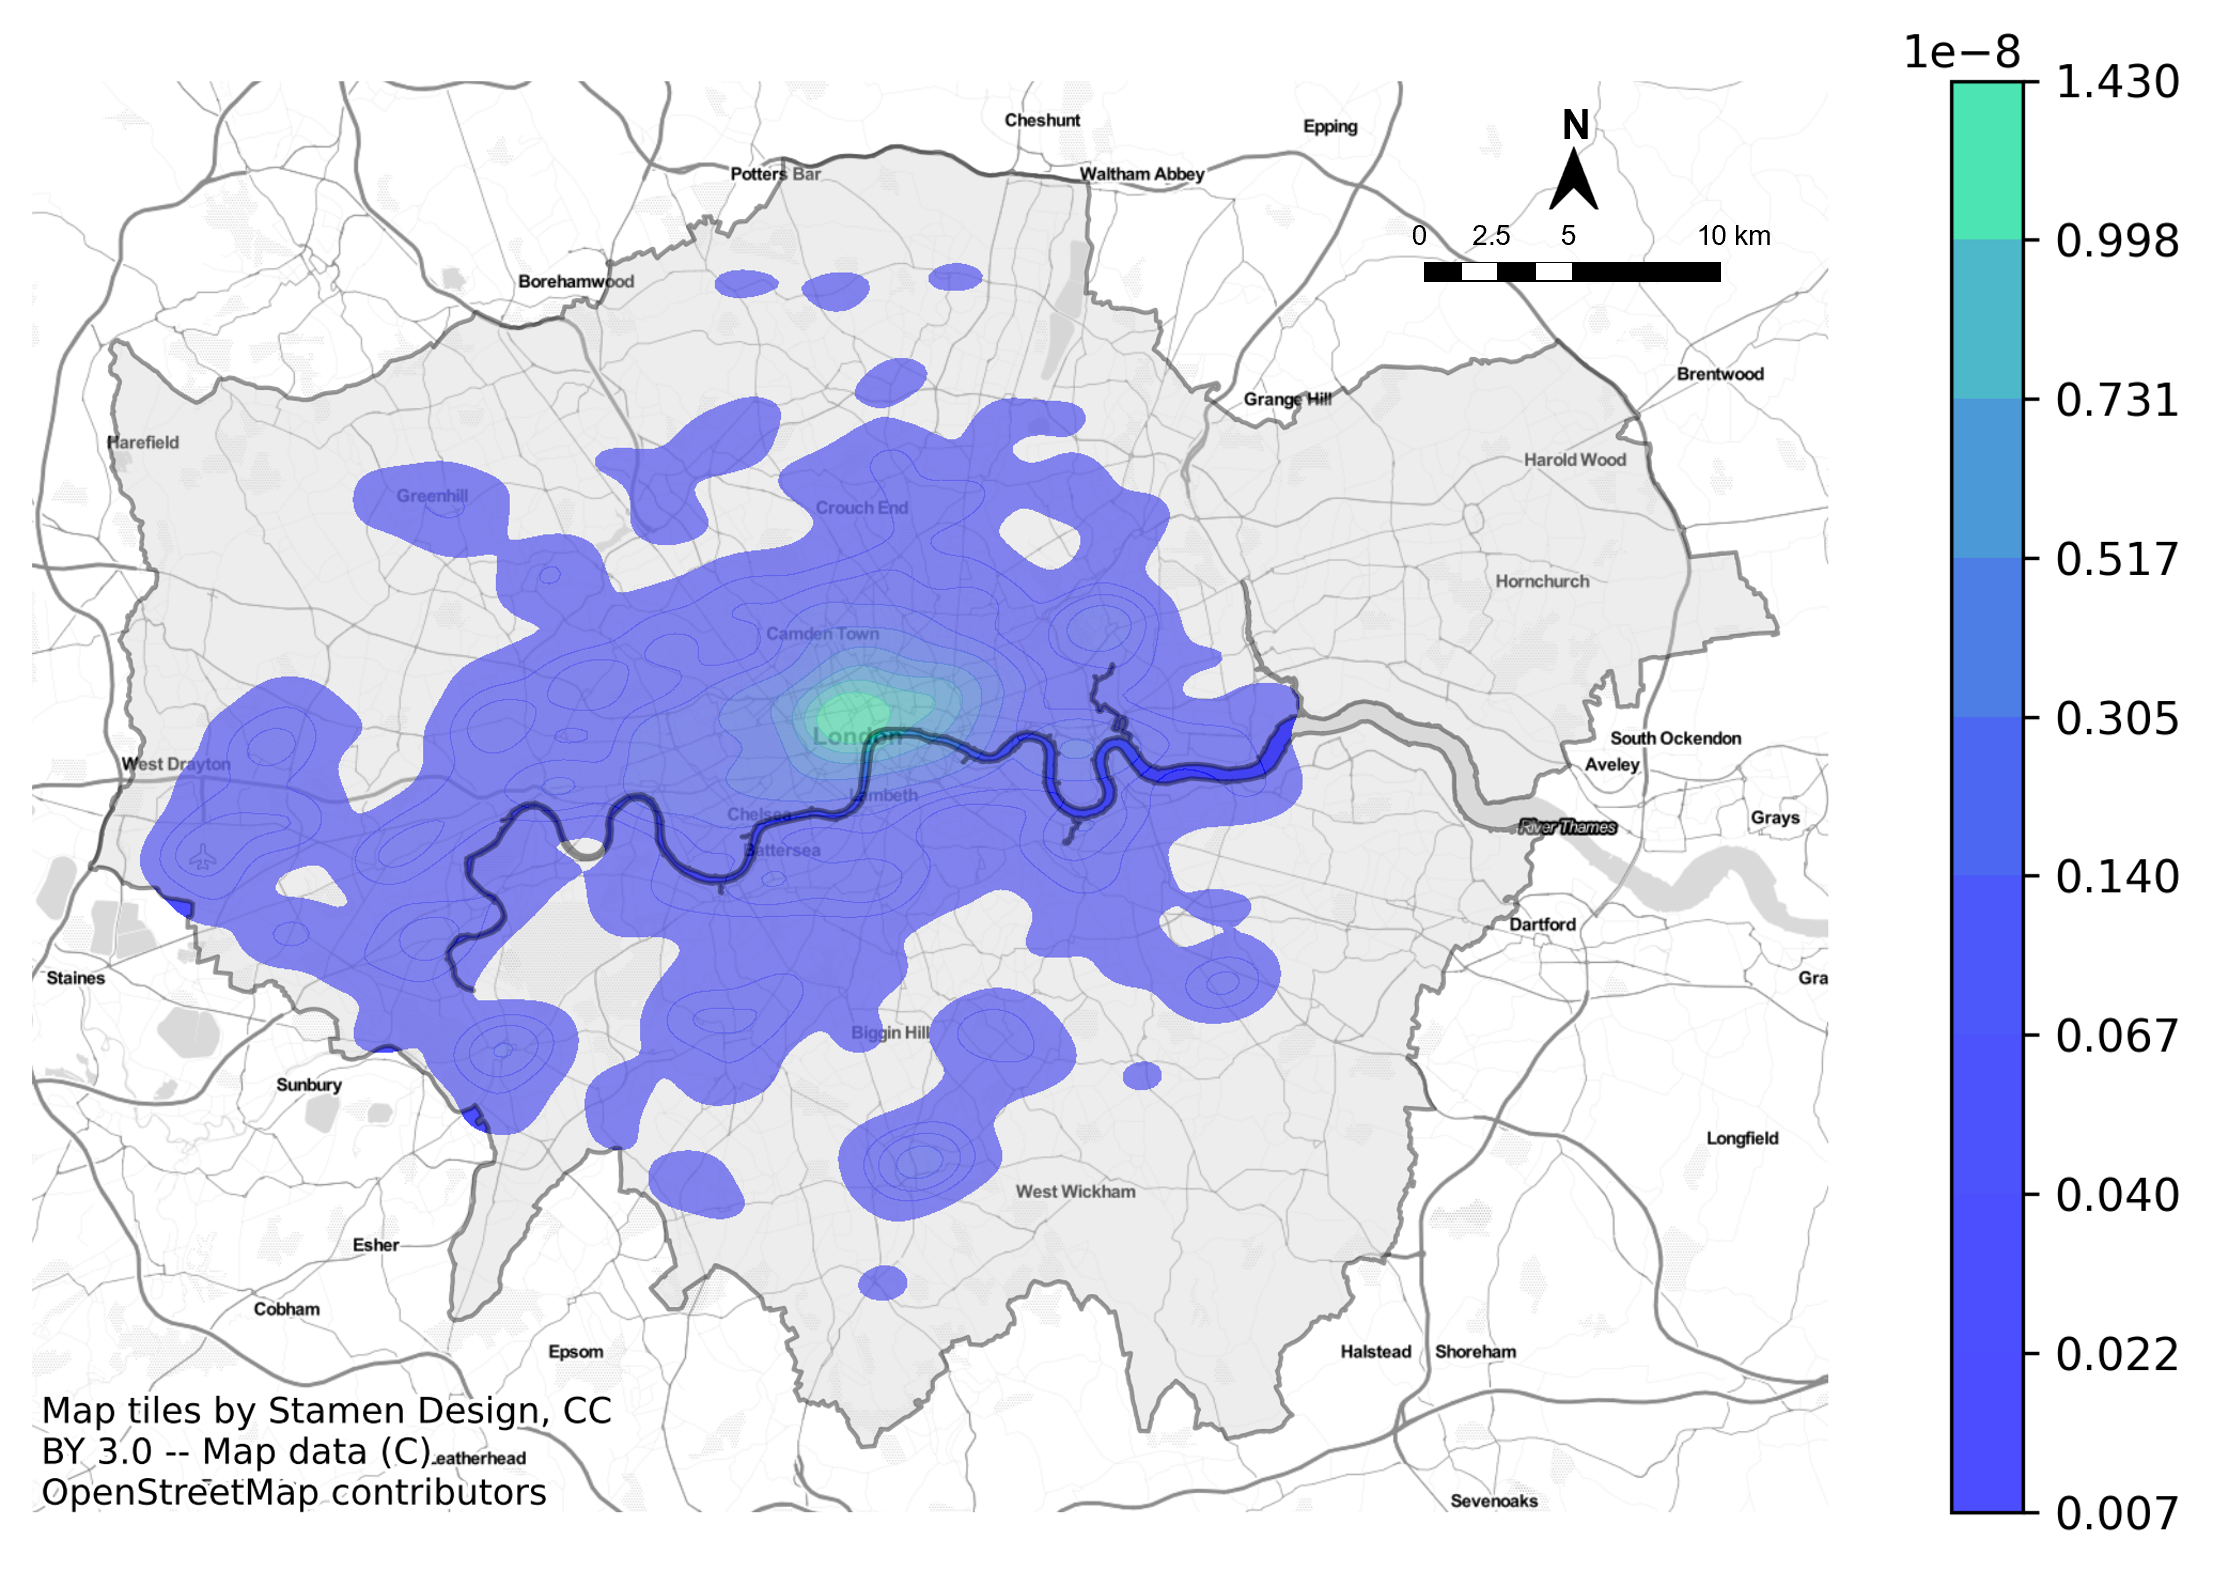
\includegraphics[width=1\linewidth]{figures/kde_locals_weekday.png} 
\caption{Locals.}
\label{fig:kde_locals_weekday}
\end{subfigure}
\begin{subfigure}{0.5\textwidth}
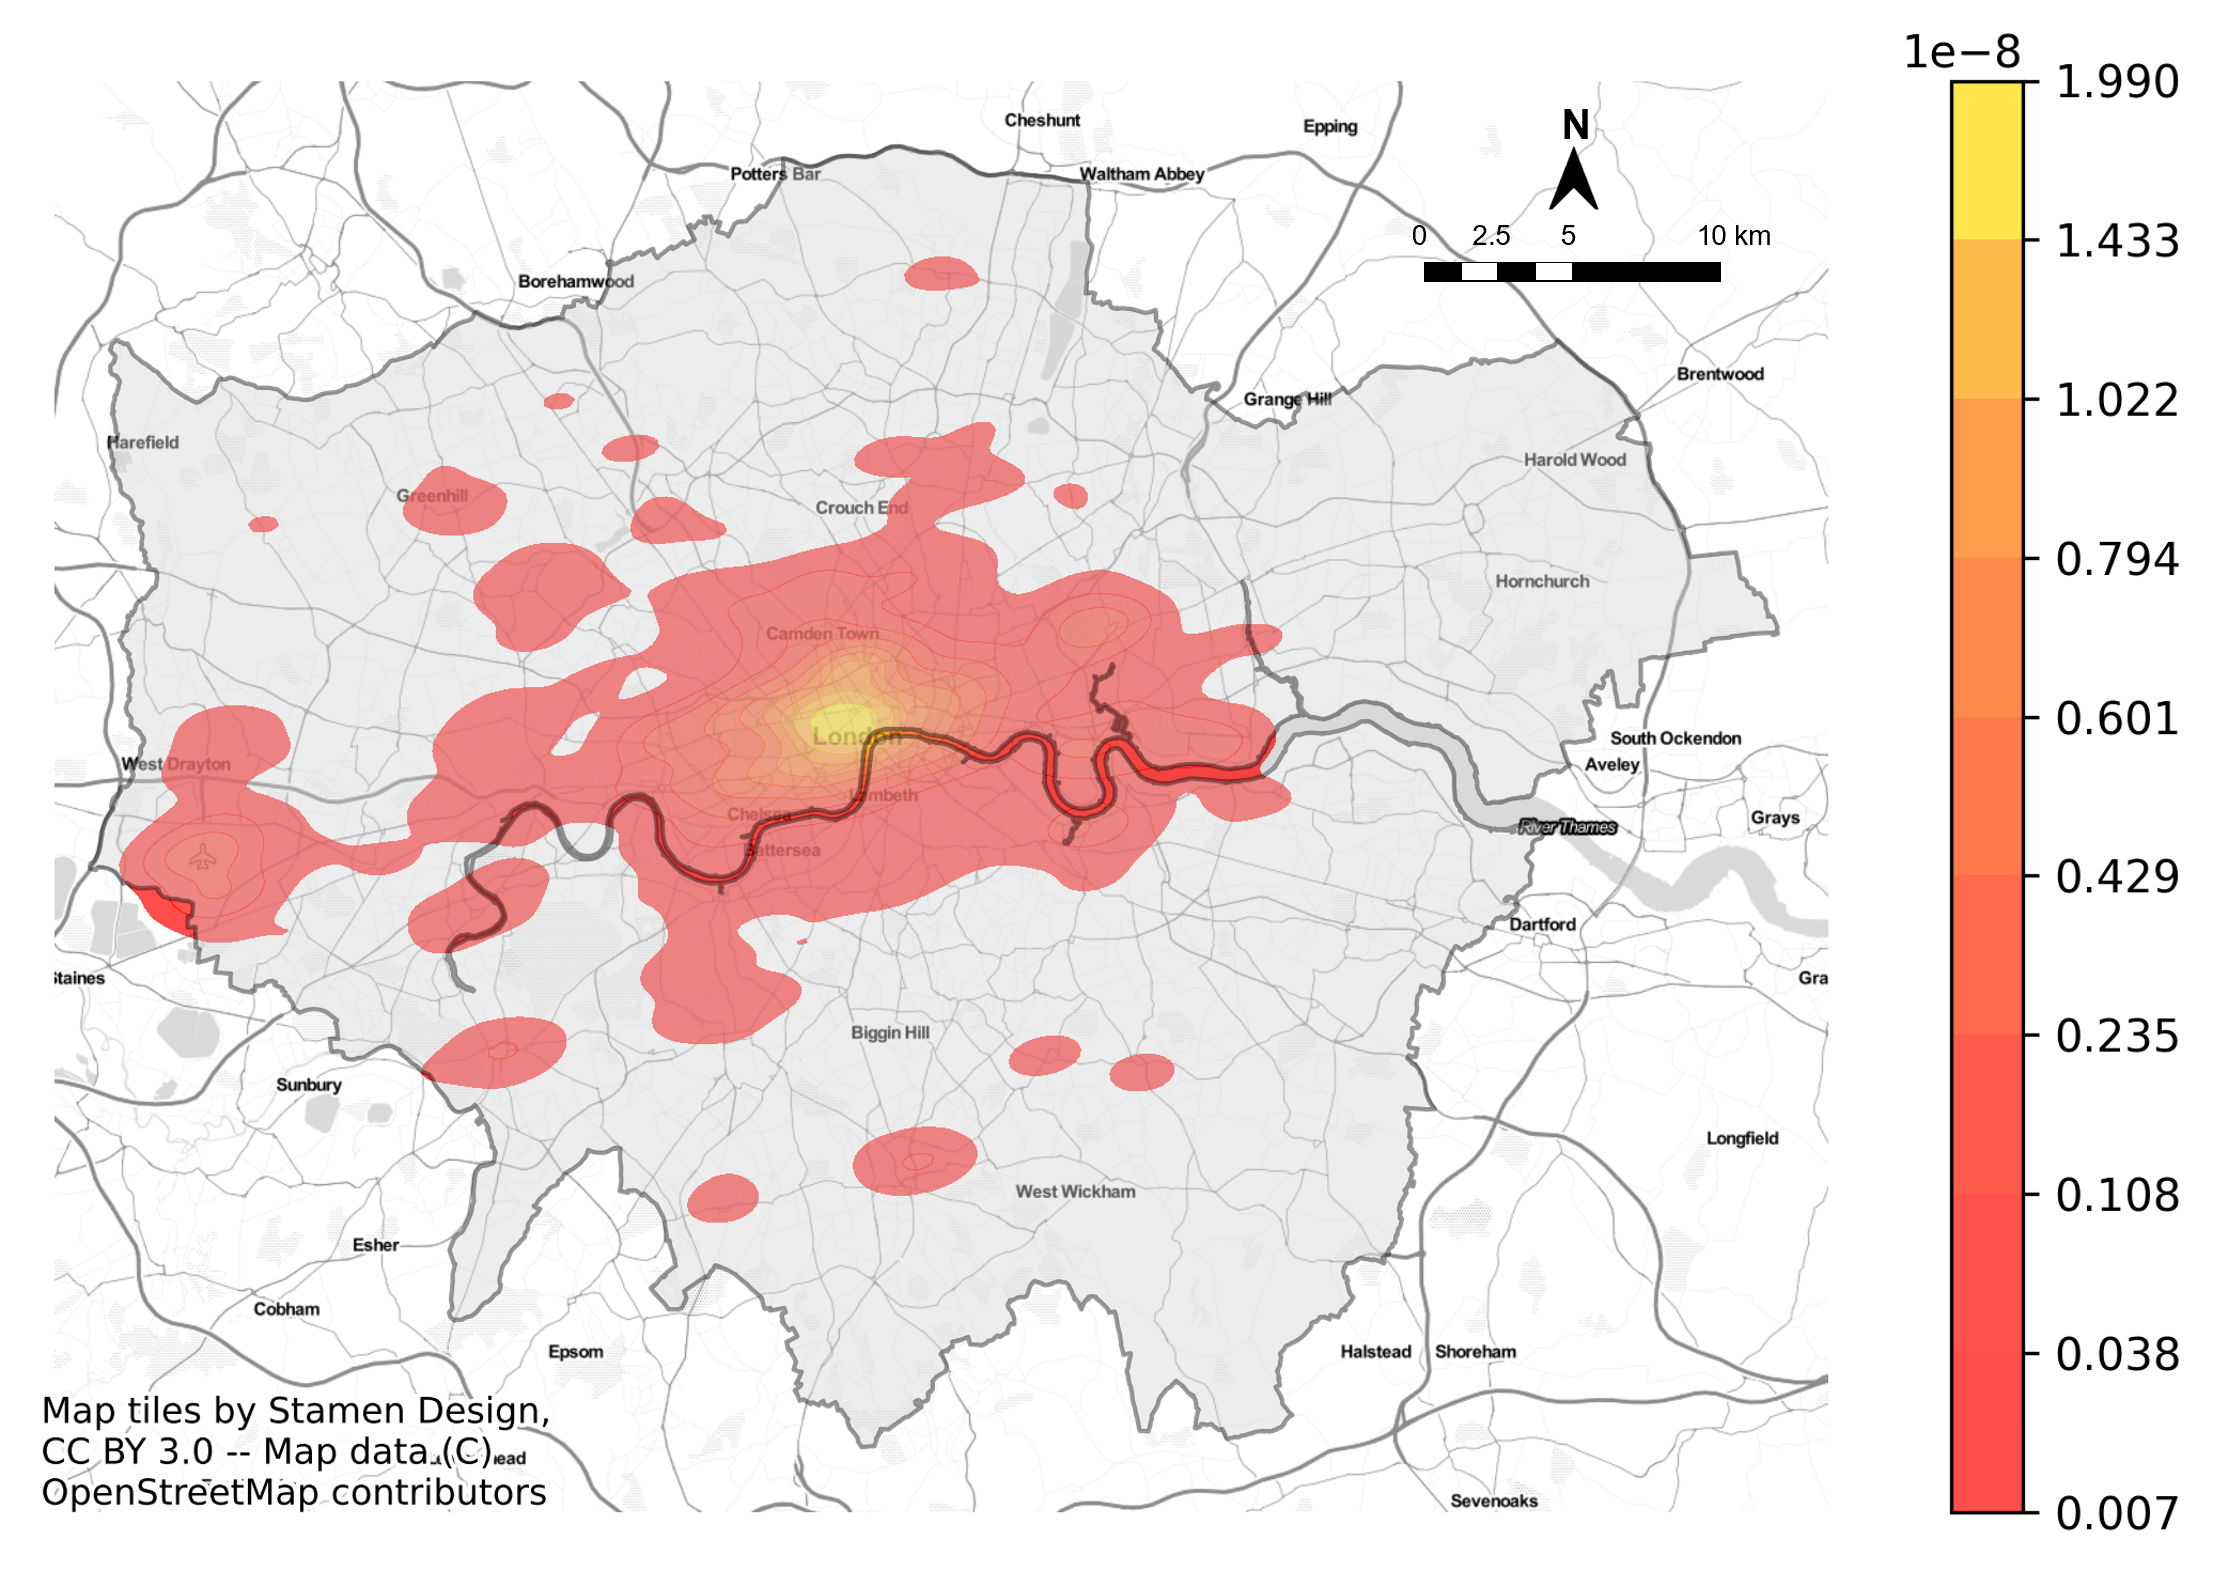
\includegraphics[width=1\linewidth]{figures/kde_tourists_weekday.png}
\caption{Tourists.}
\label{fig:kde_tourists_weekday}
\end{subfigure}

\caption{Kernel density estimation of Foursquare check-ins on weekdays.} \label{fig:kde_weekday}
\end{figure}

% weekend & comparison
On weekends, locals and tourists share fewer check-ins across London compared to weekdays (Figure~\ref{fig:kde_weekend}). Locals keep visiting both central London and various outskirts boroughs as they do on weekdays.  Conversely, the visiting areas of tourists shrink to the inner part of London, sharing fewer check-ins in the outer boroughs. In general, both locals and tourists exhibit a decrease in check-in density on weekends. The outskirts boroughs keep attracting locals throughout the week, while tourists focus their activities on the city center.

\begin{figure}[!h]

\begin{subfigure}{0.5\textwidth}
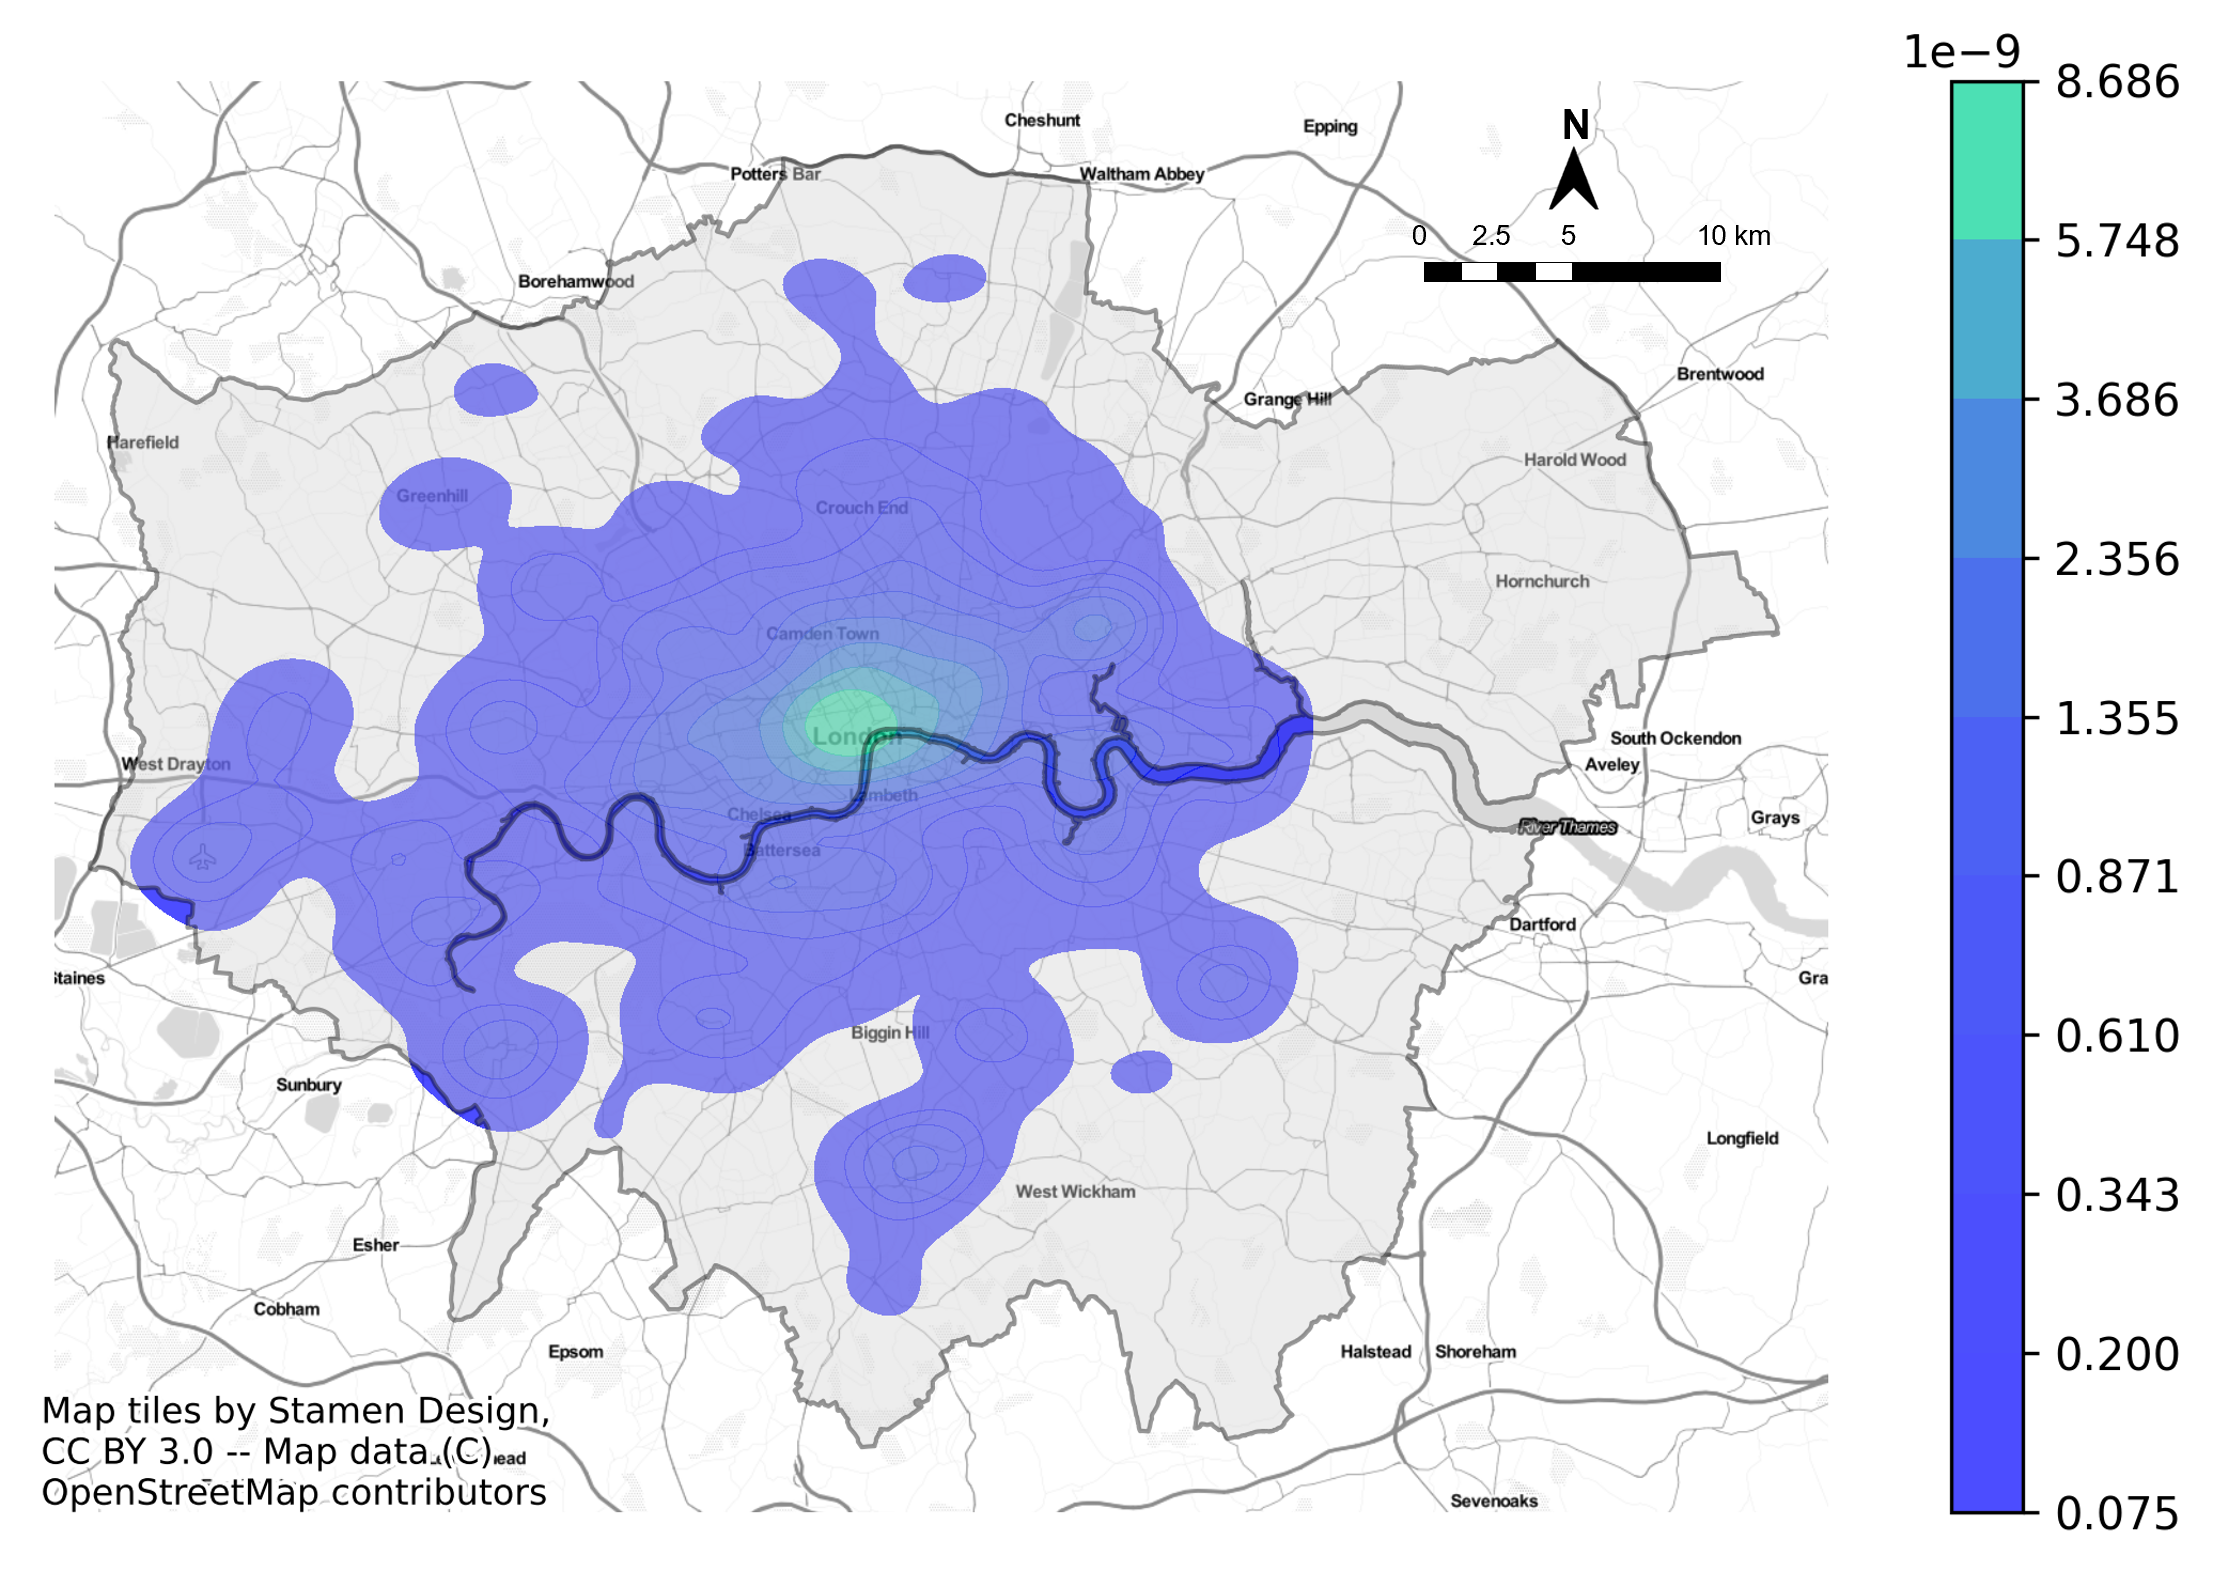
\includegraphics[width=1\linewidth]{figures/kde_locals_weekend.png} 
\caption{Locals.}
\label{fig:kde_locals_weekend}
\end{subfigure}
\begin{subfigure}{0.5\textwidth}
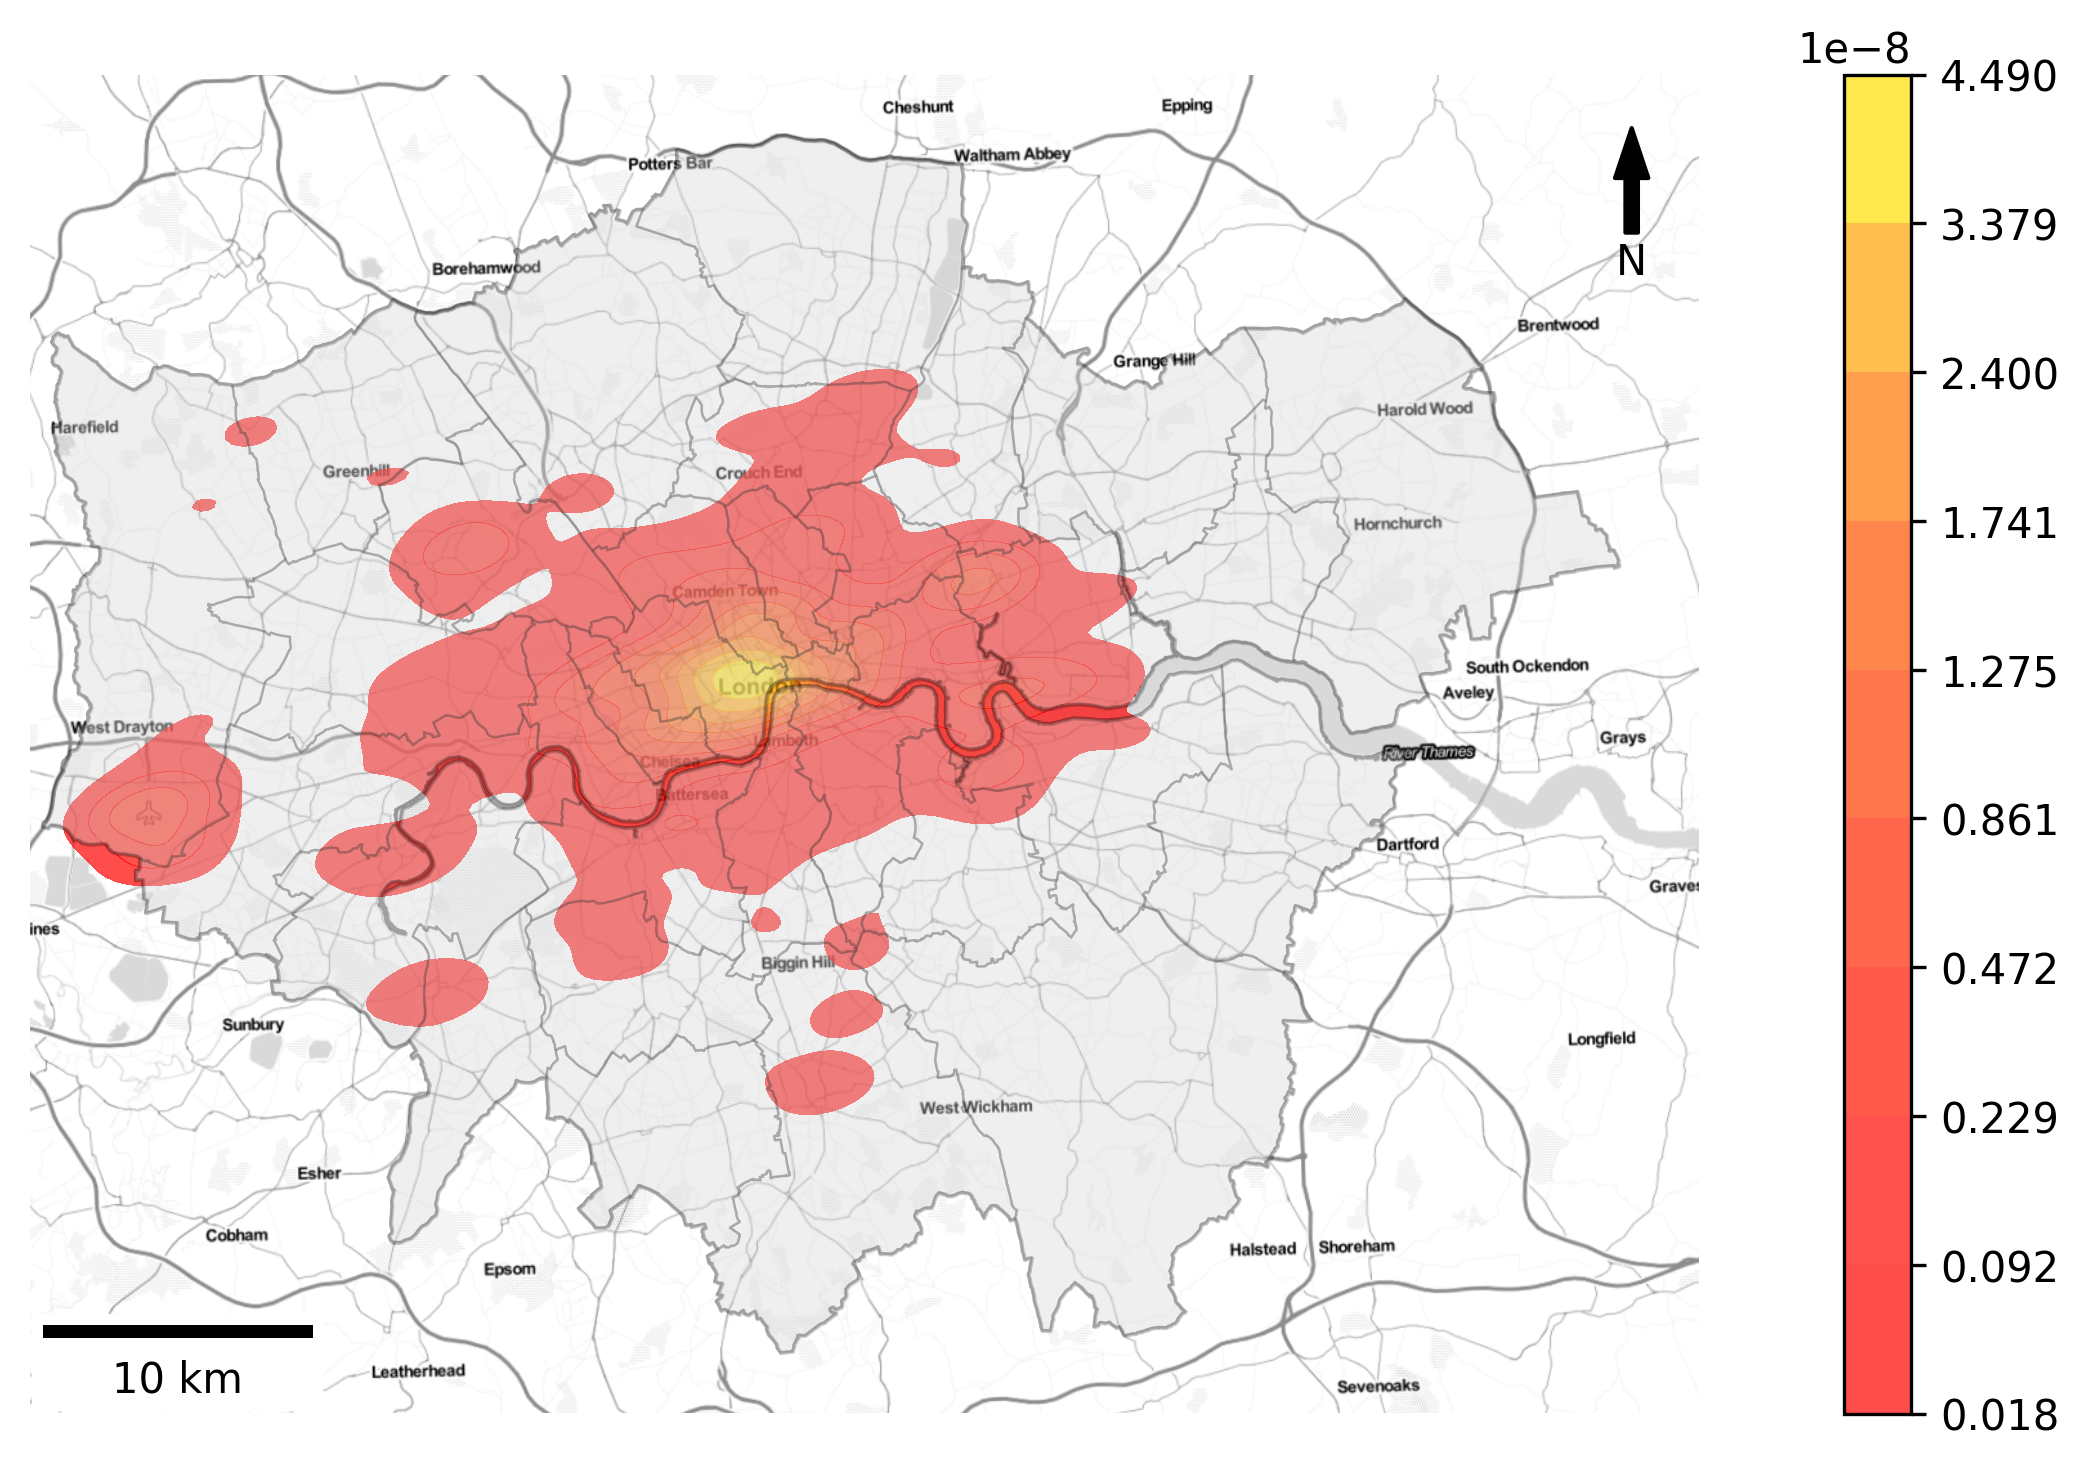
\includegraphics[width=1\linewidth]{figures/kde_tourists_weekend.png}
\caption{Tourists.}
\label{fig:kde_tourists_weekend}
\end{subfigure}

\caption{Kernel density estimation of Foursquare check-ins on weekends.} \label{fig:kde_weekend}
\end{figure}


% ====================== | Mixture of Locals and Tourists in Hotspots | ======================
\subsubsection{Mixture of Locals and Tourists in Hotspots}

% ============== Daytime vs. Nighttime ==============
\subsubsubsection{Daytime vs. Nighttime}
% difference ratio
Figure~\ref{fig:raster_diff_day} shows the difference ratio between locals and tourists within each raster throughout the day. The difference ratio reveals the mixture degree of check-ins shared by locals and tourists. A positively higher difference ratio indicates a larger activity density of tourists, while a negatively lower difference ratio suggests a higher concentration of locals' activities. During the daytime, most areas across London, except for the city center, receive similar popularity from both groups. Though both locals and tourists share a large number of check-ins in the city center, they have distinct areas of interest. Tourists tend to cluster in Westminster and Camden, while locals are more concentrated in the eastern region, particularly in the City of London, and the Canary Wharf in Tower Hamlets. These findings align with the observations in Section \ref{hotspots}. In addition, the hotspot around Heathrow Airport displays a positive value of difference ratio, indicating a higher activity density of tourists (Figure~\ref{fig:raster_diff_daytime}). Moving to the nighttime, the city center, especially Westminster, becomes increasingly popular among tourists, while the area around the City of London shows a balanced presence of locals and tourists, indicating reduced activities of locals during the nighttime. Furthermore, the difference ratio of some outskirts rasters becomes negative when it comes to the nighttime, indicating an outflux of locals from the city center (Figure~\ref{fig:raster_diff_nighttime}).

% significant difference ratio - category distribution 
The category distribution of check-ins within rasters with significant difference ratios (greater than 0.01 or less than -0.01) is represented in Figure~\ref{fig:diff_pop_category_day}. During the daytime, tourists demonstrate a preference for restaurants, transportation places, and shopping places, while locals show a higher inclination towards professional places, restaurants, and entertainment places (Figure~\ref{fig:diff_pop_category_daytime}). In terms of the nighttime, tourists exhibit a great interest in entertainment places while maintaining their preference for restaurants and transportation places. Locals, on the other hand, shift their focus from professional places to entertainment places while still showing interest in restaurants (Figure~\ref{fig:diff_pop_category_nighttime}). 
Table~\ref{tab:popular_venues_touristspop_daytime} - Table~\ref{tab:popular_venues_localspop_nighttime} in Appendix \ref{appendix} list the top 10 popular venues within rasters with significant difference ratios. Popular daytime venues for tourists include transportation hubs like London King's Cross Railway Station, luxury department stores like Harrods, and prominent public squares like Trafalgar Square. On the other hand, locals during the daytime tend to visit more professional venues like Google Campus - London and other companies, as well as restaurants around Shoreditch. Regarding the nighttime, popular venues for both locals and tourists include nightclubs and pubs, alongside transportation hubs.


\begin{figure}[!h]

\begin{subfigure}{0.5\textwidth}
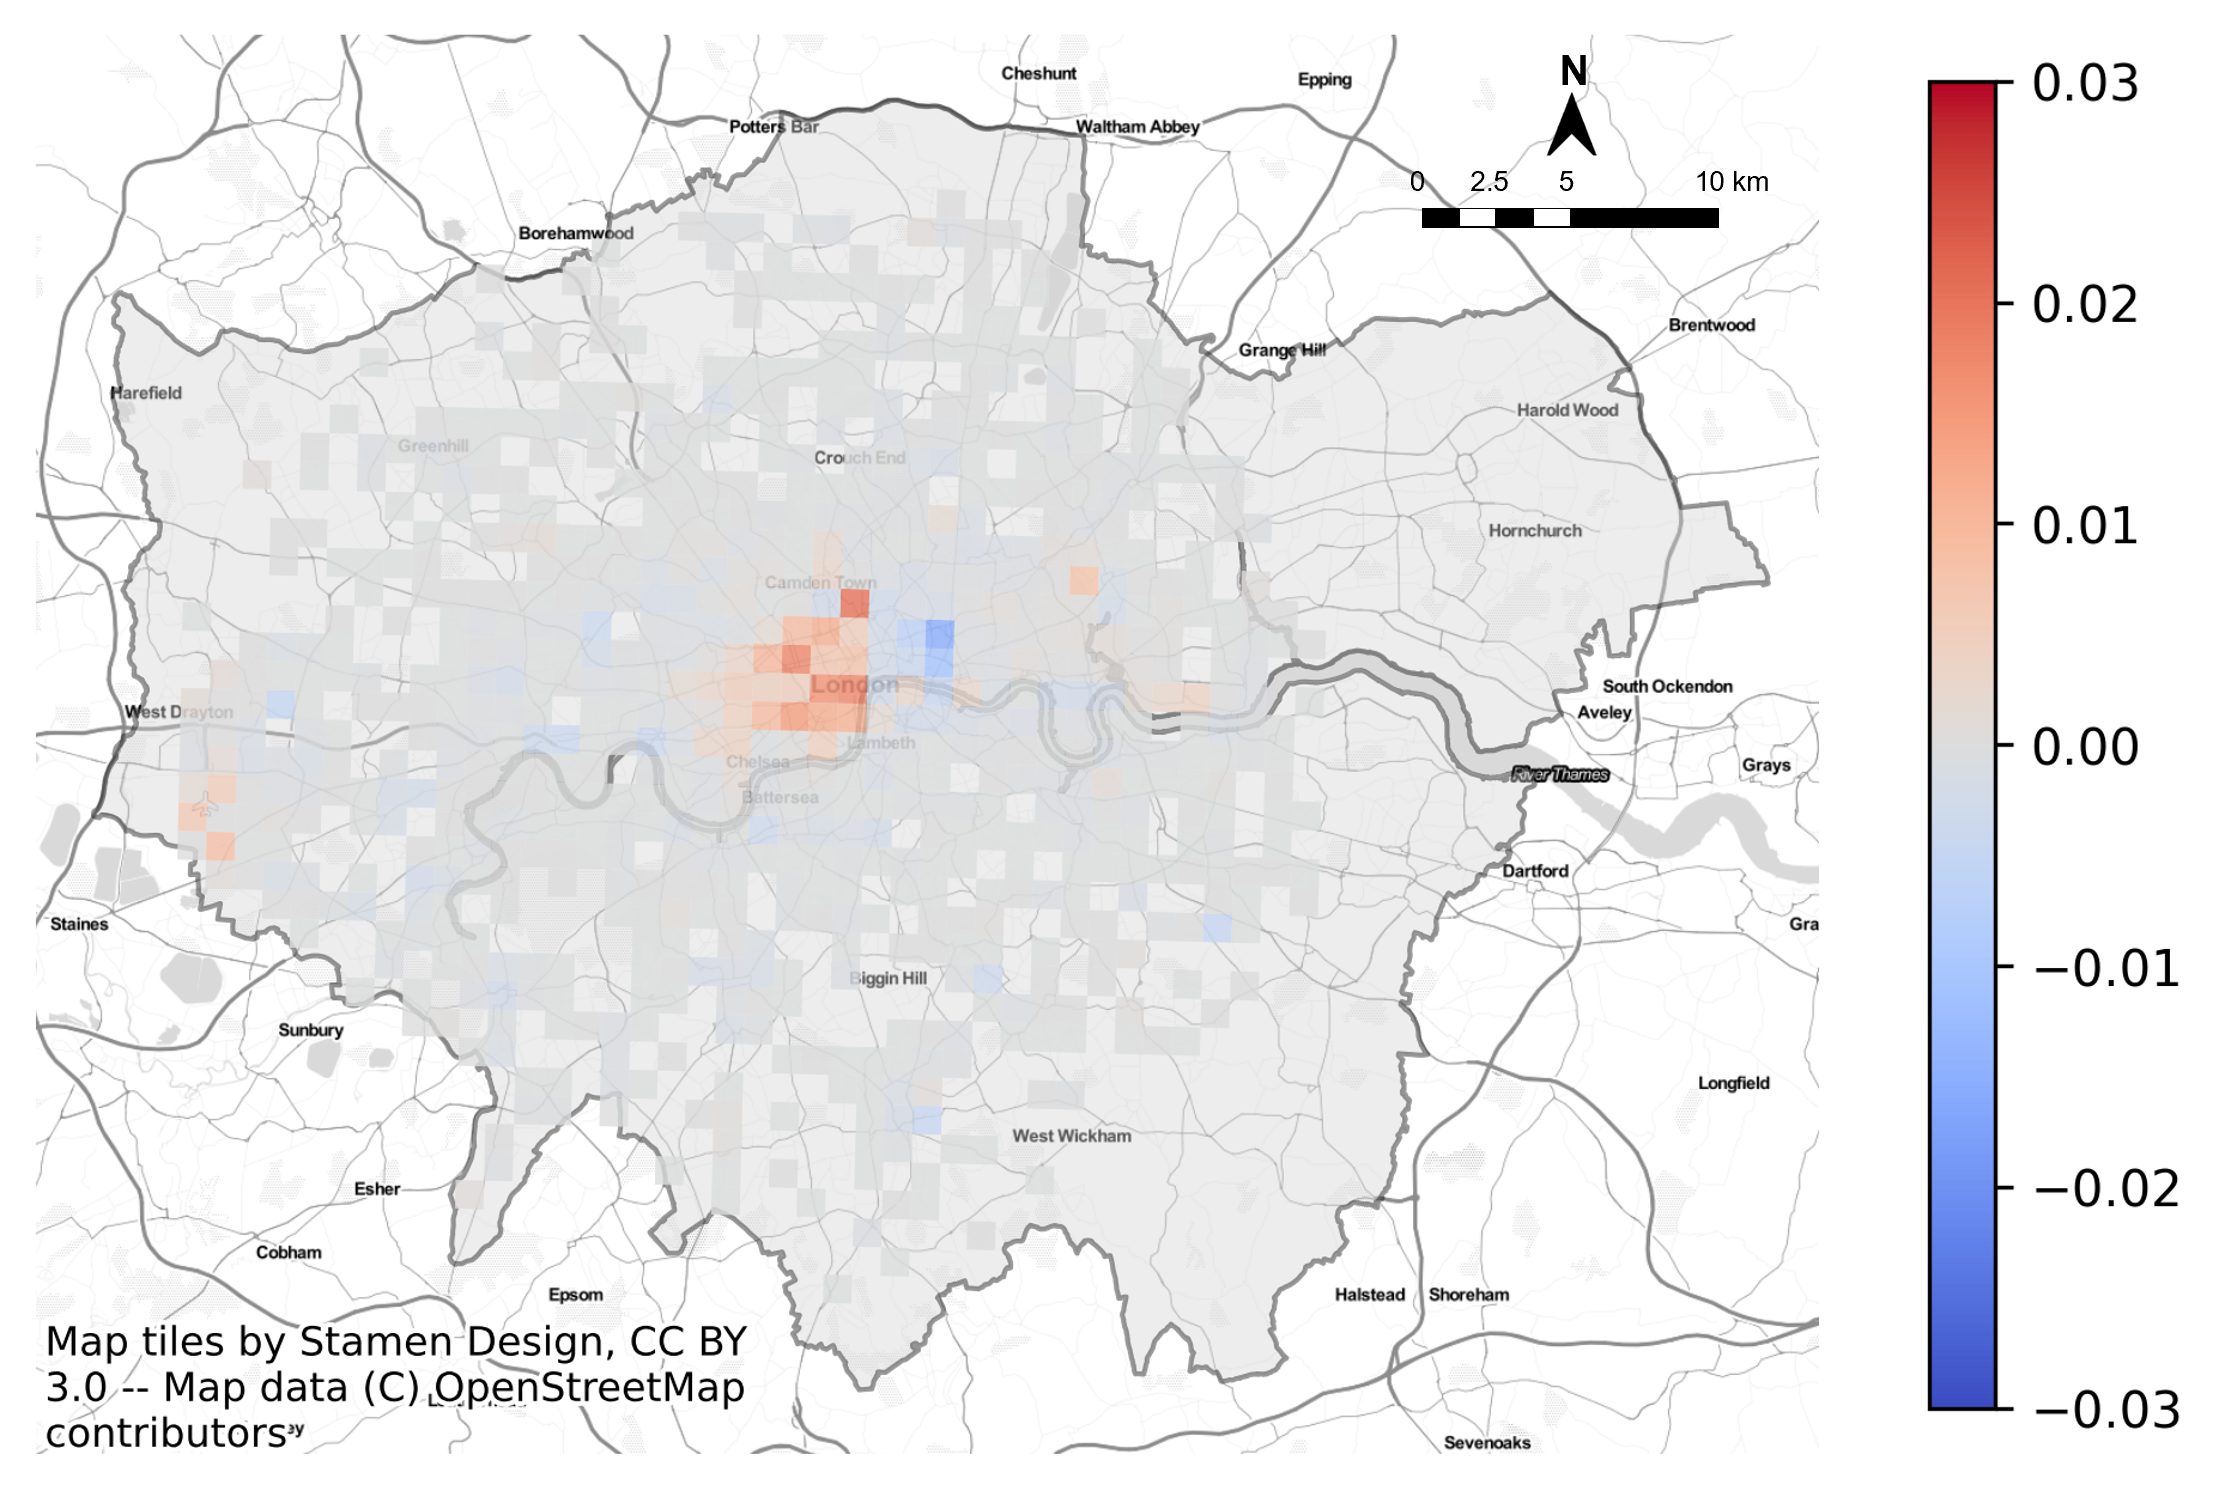
\includegraphics[width=1\linewidth]{figures/raster_diff_daytime.png} 
\caption{Daytime.}
\label{fig:raster_diff_daytime}
\end{subfigure}
\begin{subfigure}{0.5\textwidth}
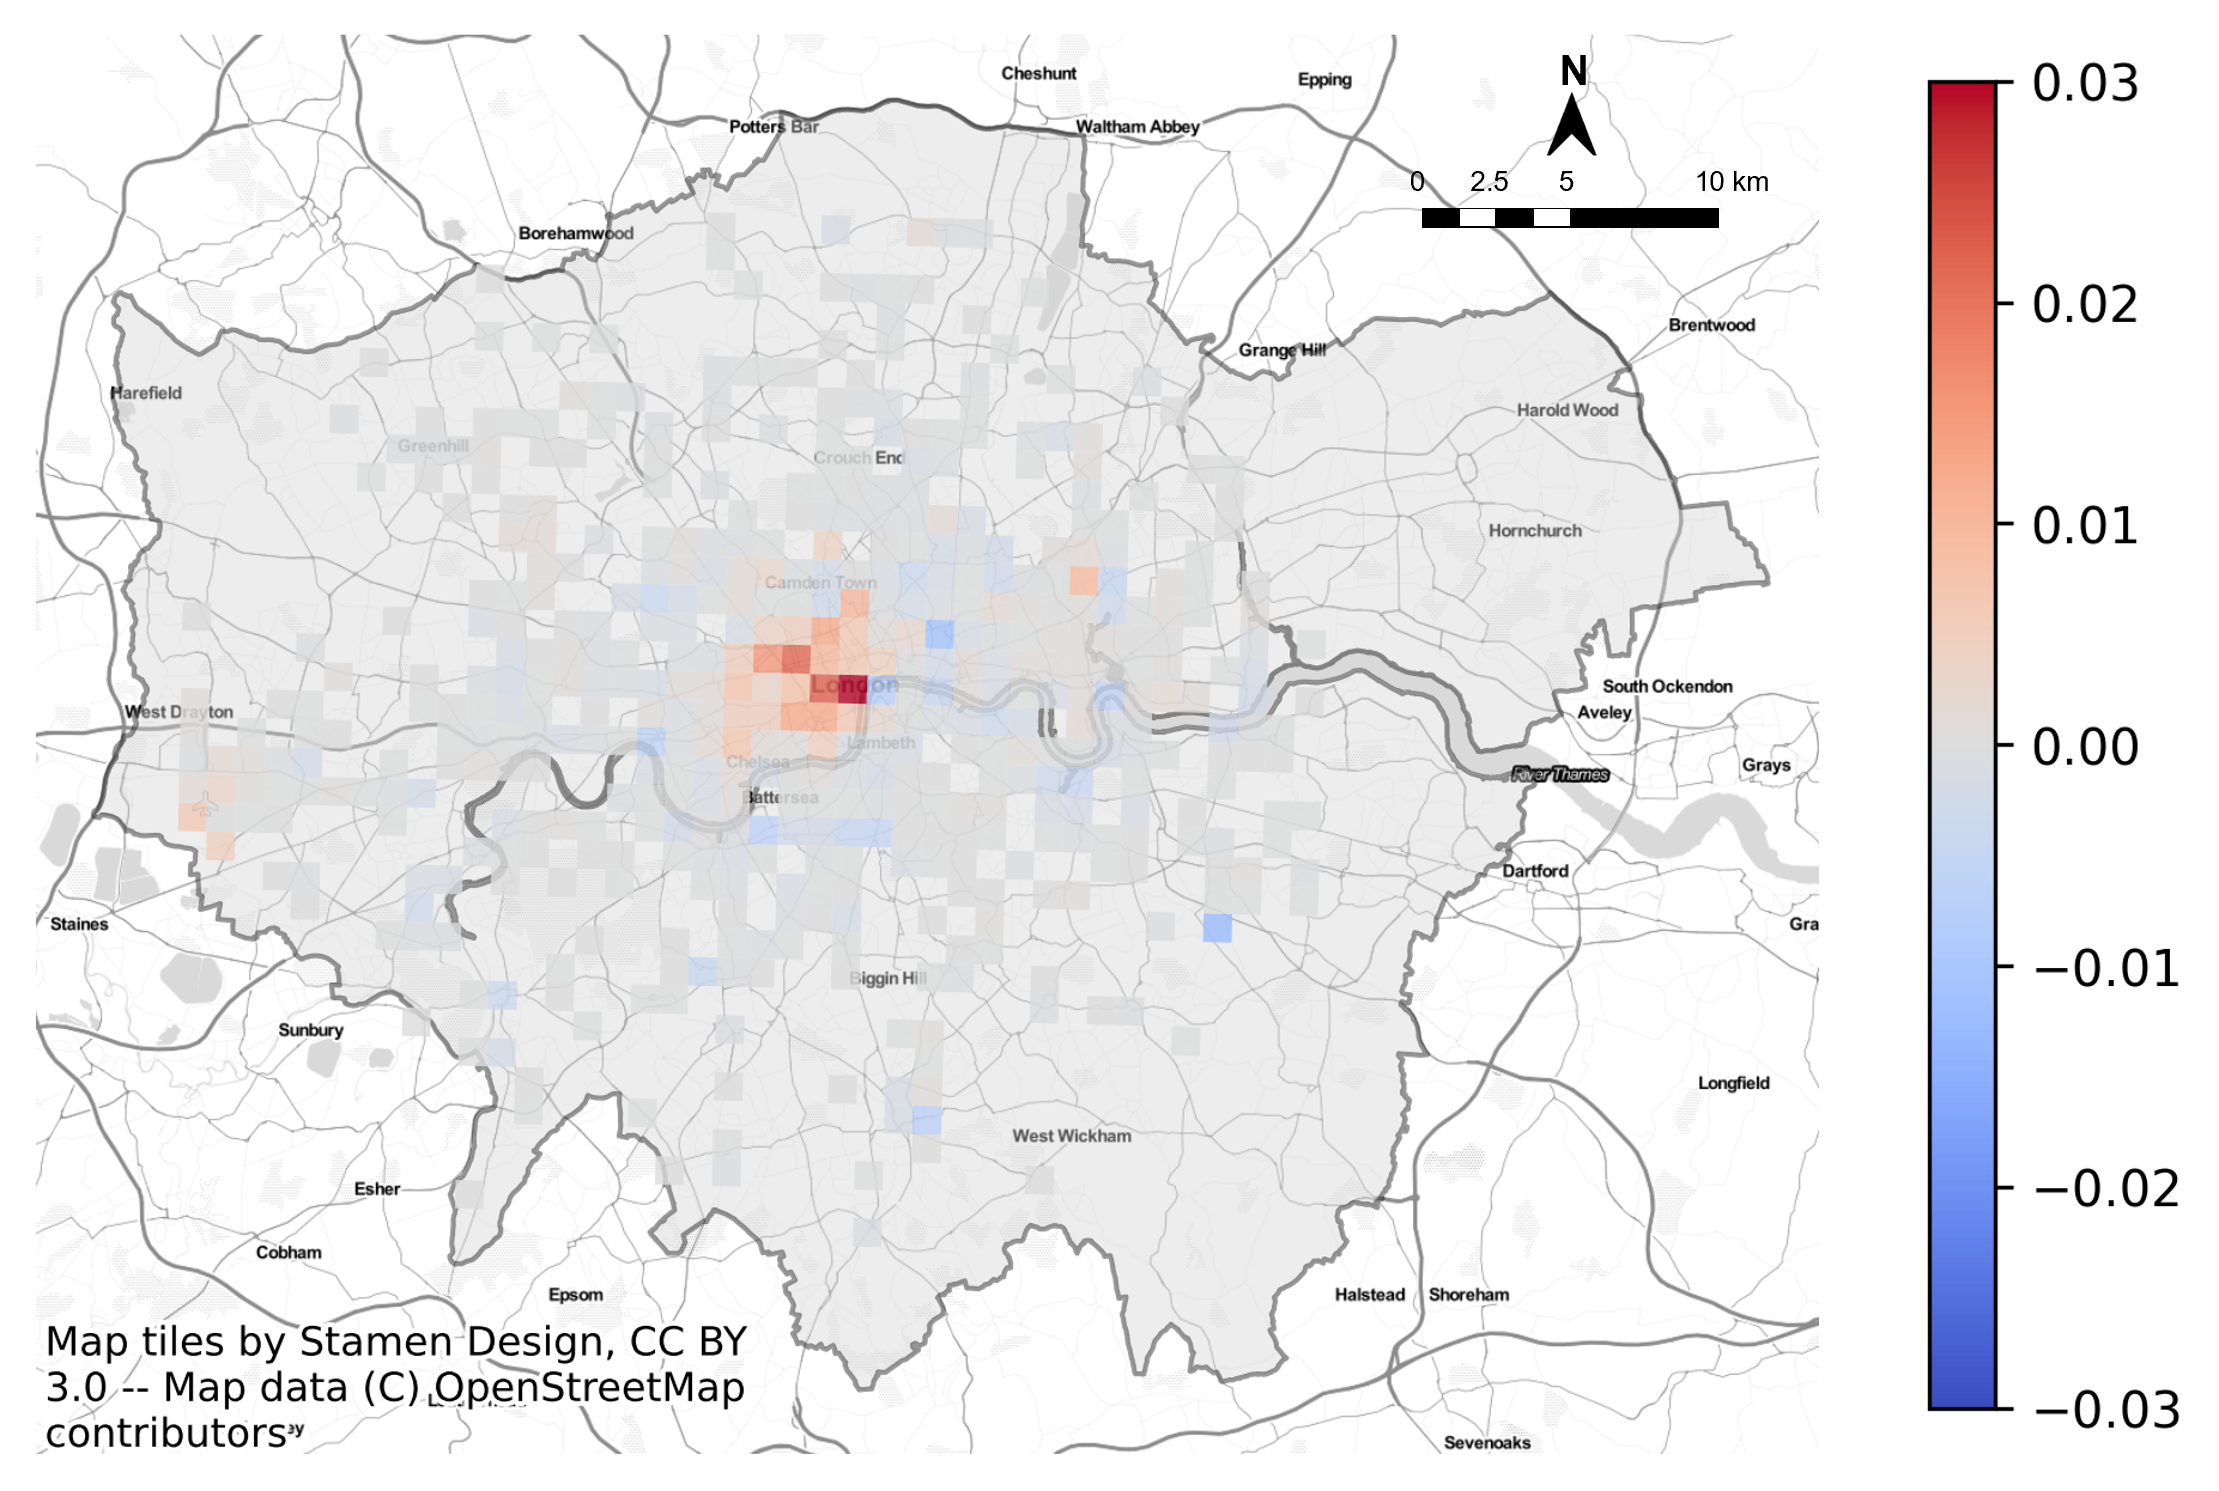
\includegraphics[width=1\linewidth]{figures/raster_diff_nighttime.png}
\caption{Nighttime.}
\label{fig:raster_diff_nighttime}
\end{subfigure}

\caption{Difference ratio of rasters during the daytime and nighttime.} \label{fig:raster_diff_day}
\end{figure}


\begin{figure}[!h]

\begin{subfigure}{0.5\textwidth}
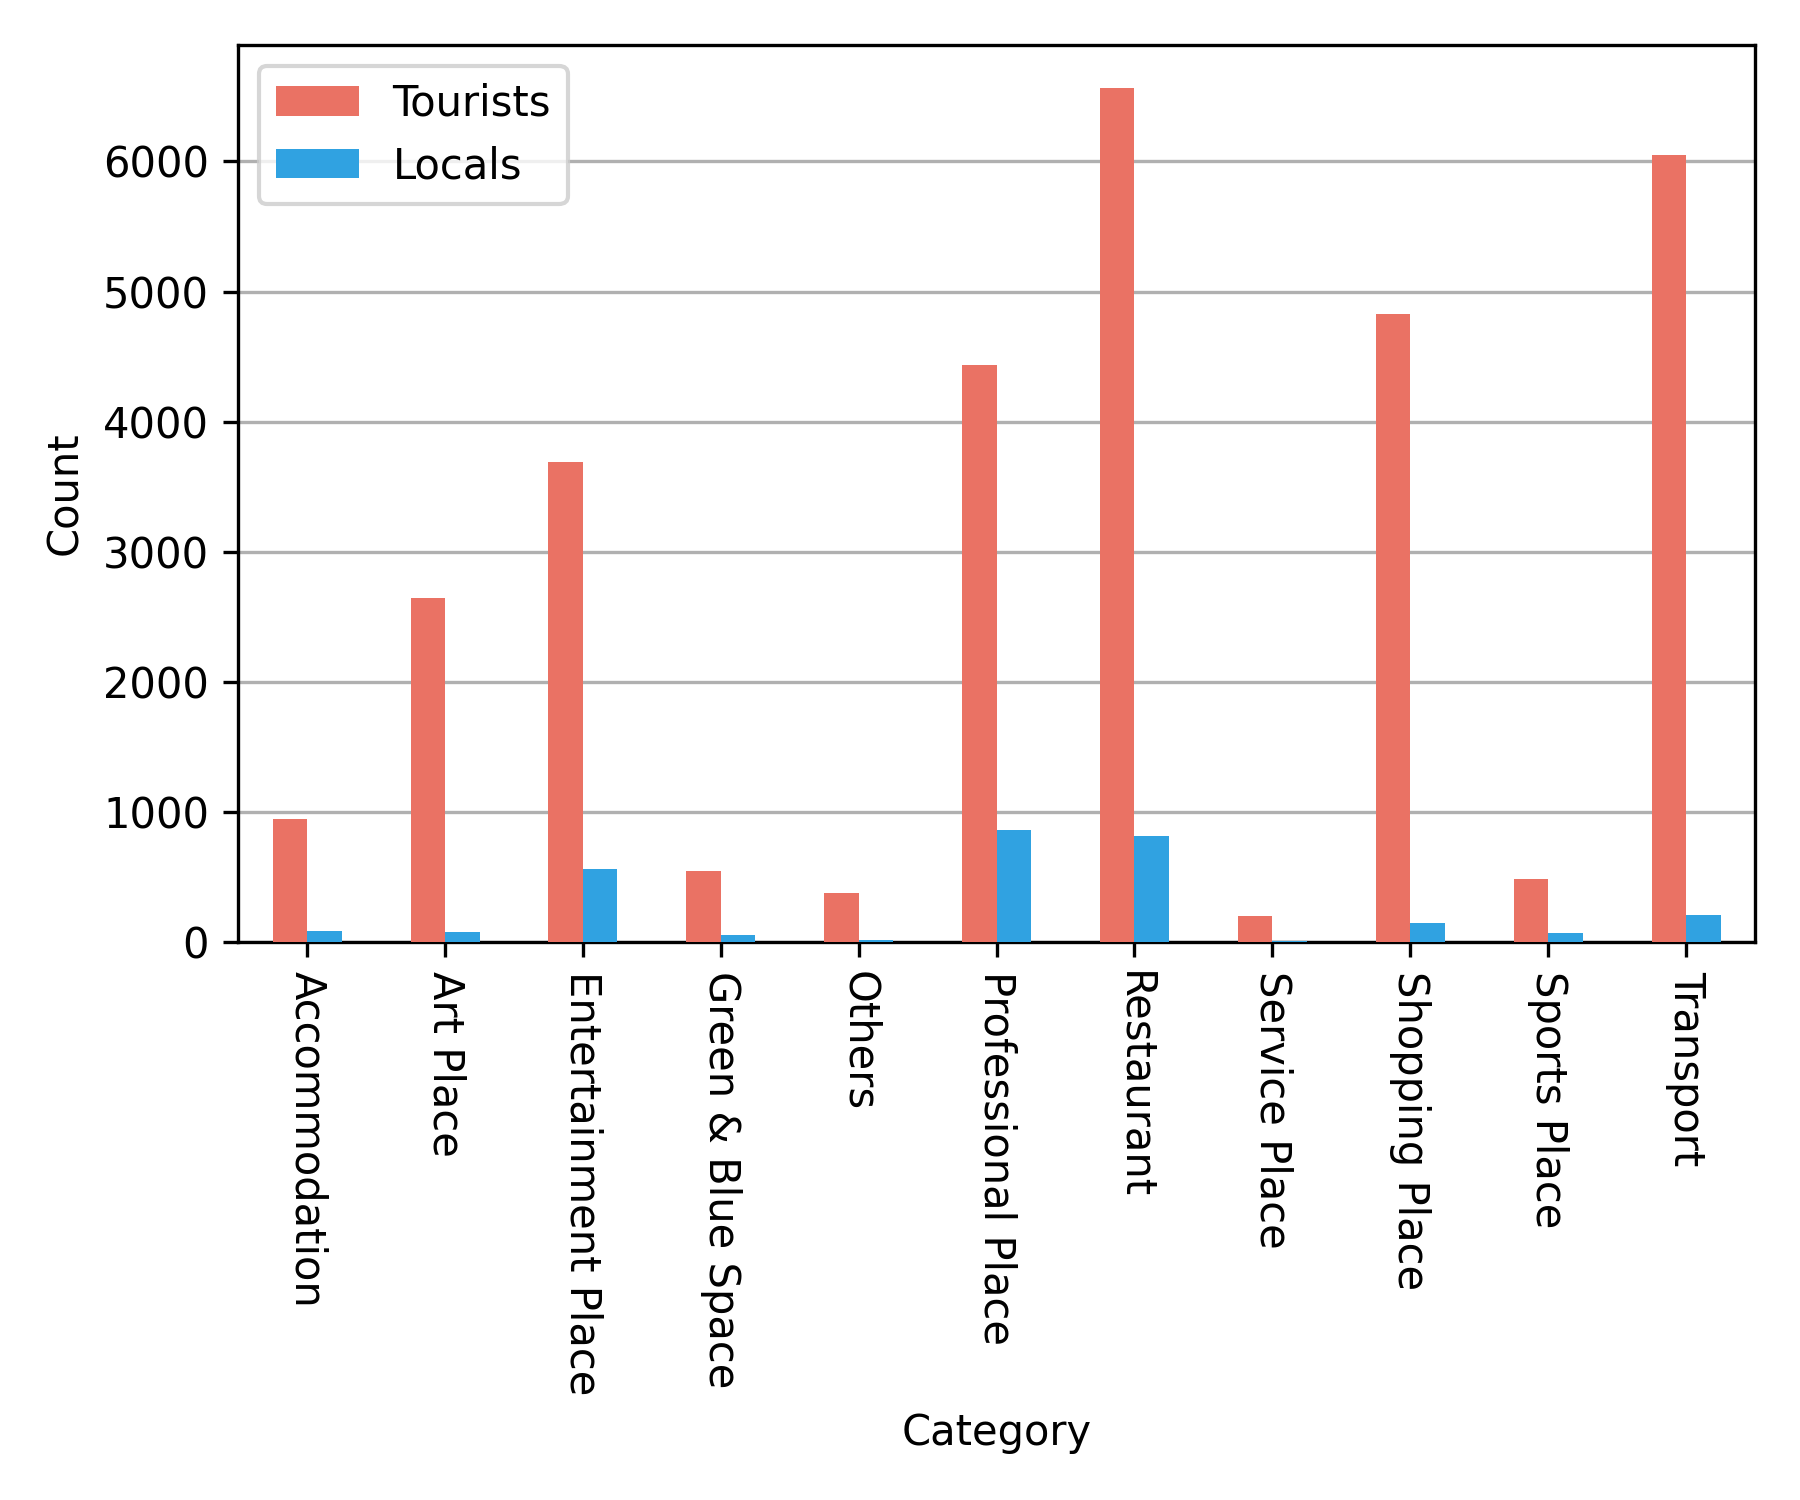
\includegraphics[width=1\linewidth]{figures/diff_pop_category_daytime.png} 
\caption{Daytime.}
\label{fig:diff_pop_category_daytime}
\end{subfigure}
\begin{subfigure}{0.5\textwidth}
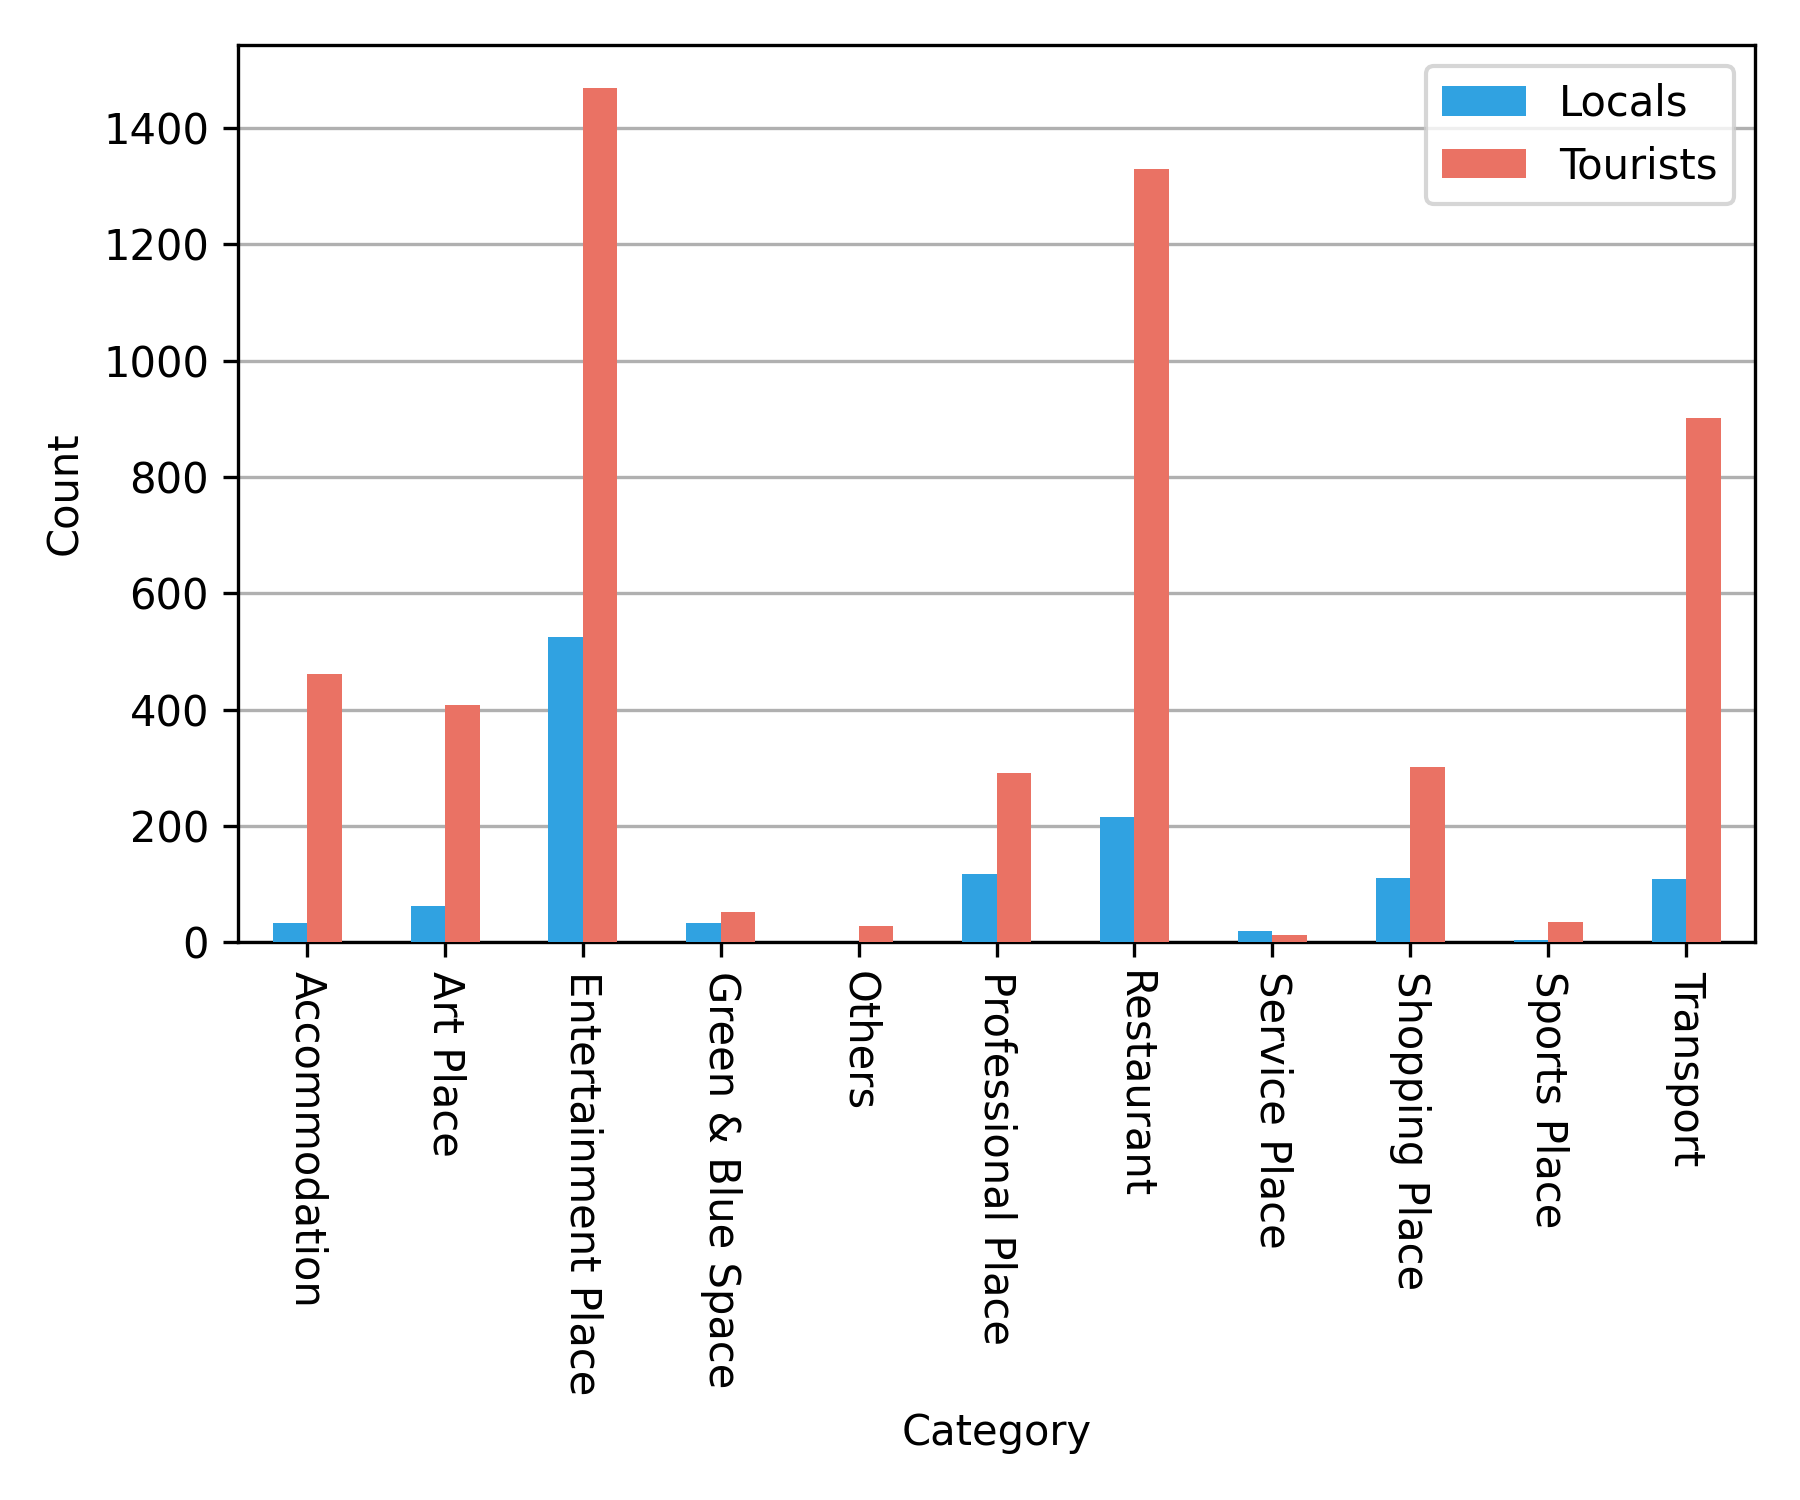
\includegraphics[width=1\linewidth]{figures/diff_pop_category_nighttime.png}
\caption{Nighttime.}
\label{fig:diff_pop_category_nighttime}
\end{subfigure}

\caption{Number of check-in categories in popular areas during the daytime and nighttime.} \label{fig:diff_pop_category_day}
\end{figure}



% ============== Weekday vs. Weekend ==============
\subsubsubsection{Weekday vs. Weekend}
% difference ratio
Figure~\ref{fig:raster_diff_week} displays the mixture degree of locals and tourists throughout the week. On weekdays, locals and tourists tend to visit distinct areas in the city center, as shown in the significant positive and negative values of difference ratio around this area. As discussed in previous sections, tourists concentrate their activities in Westminster and Camden, while locals exhibit a higher activity density towards the east, particularly around the City of London, which is a prominent business district (Figure~\ref{fig:raster_diff_weekday}). Moving on to weekends, the hotspot of tourists in the city center becomes more popular among tourists, with higher difference ratios in relevant rasters. Conversely, the increased difference ratios in the locals' hotspot in the city center indicate a reduced proportion of locals, suggesting a decrease in local visits to this area on weekends. In addition, some outskirts rasters experience a decrease in difference ratios, meaning that locals on weekends are more scattered across London compared to weekdays (Figure~\ref{fig:raster_diff_weekend})

% significant difference ratio - category distribution 
The category distribution of check-ins in rasters with significant difference ratios (greater than 0.01 or less than -0.01) is depicted in Figure~\ref{fig:diff_pop_category_week}. On weekdays, both tourists and locals display a preference for entertainment places, professional places, restaurants, and transportation places (Figure~\ref{fig:diff_pop_category_weekday}). But when it comes to the weekends, tourists switch interests from professional places to shopping places, with consistent interests in three other categories. Locals, on the other hand, reduce their visits to professional places and transportation places (Figure~\ref{fig:diff_pop_category_weekend}). In terms of the popular venues in rasters with significant difference ratios, tourists exhibit a consistent preference for transportation hubs, public squares, and luxury departments throughout the week. While locals shift their visits towards more leisure venues like coffee shops and bars on weekends, rather than company establishments on weekdays. For more detailed information, please refer to Table~\ref{tab:popular_venues_touristspop_weekday} - Table~\ref{tab:popular_venues_localspop_weekend} in Appendix \ref{appendix}.


\begin{figure}[!h]

\begin{subfigure}{0.5\textwidth}
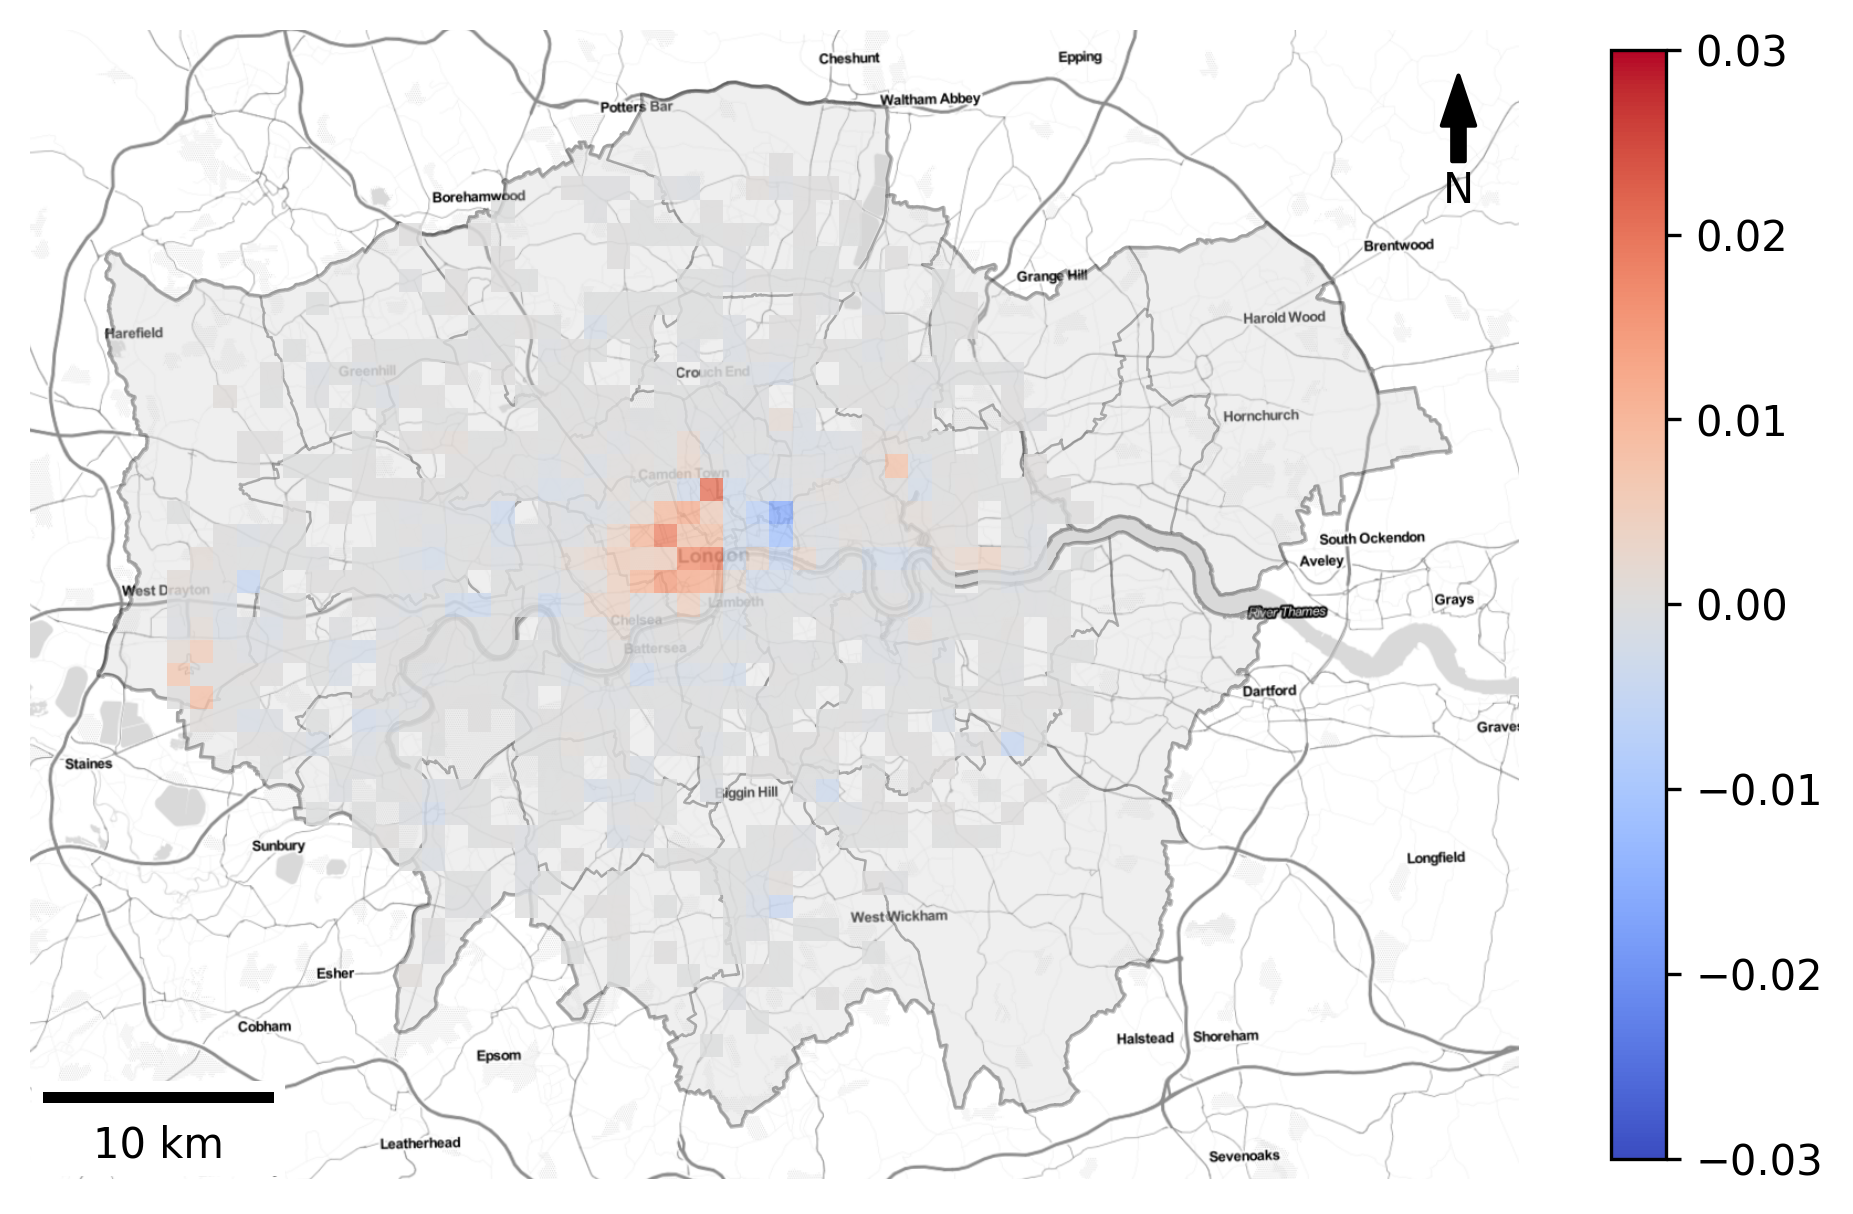
\includegraphics[width=1\linewidth]{figures/raster_diff_weekday.png} 
\caption{Weekday.}
\label{fig:raster_diff_weekday}
\end{subfigure}
\begin{subfigure}{0.5\textwidth}
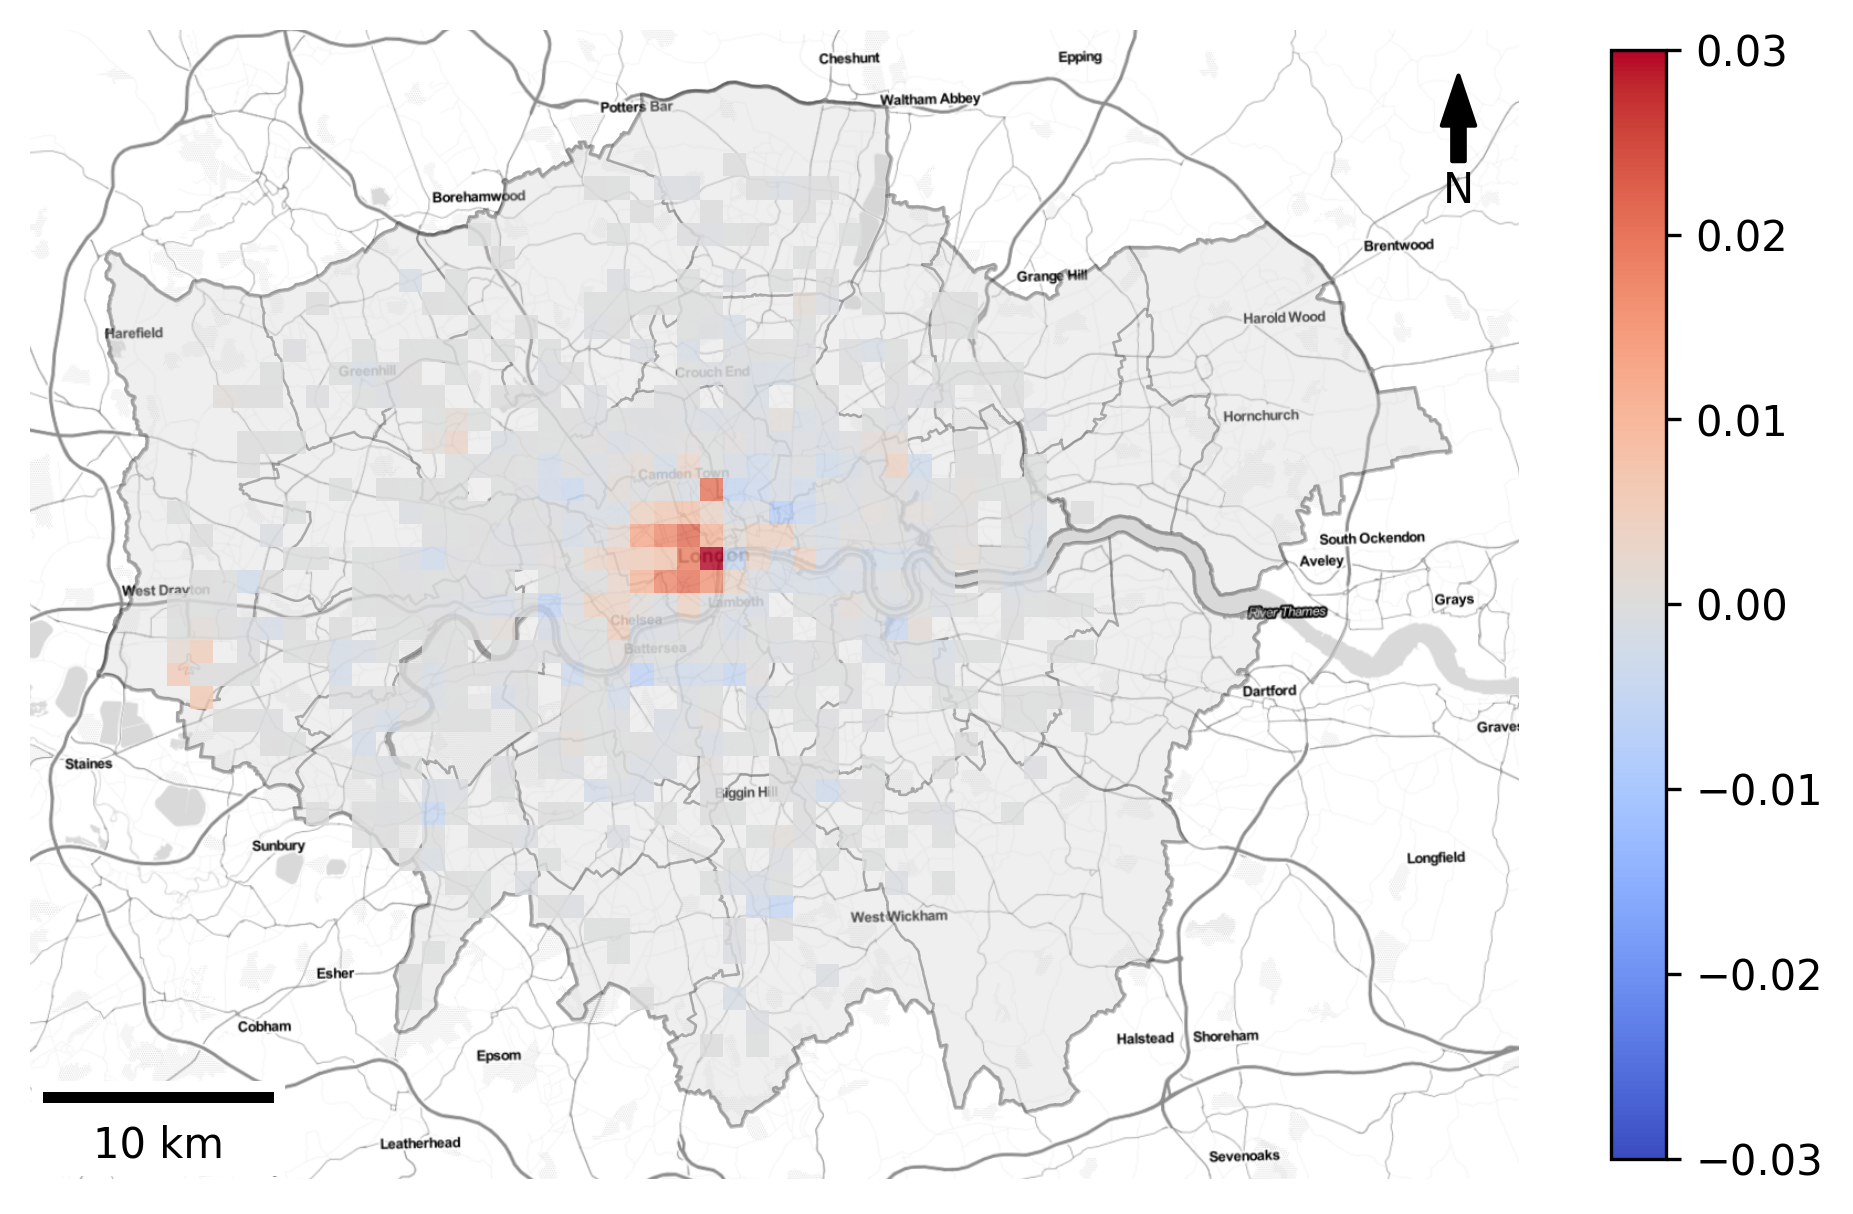
\includegraphics[width=1\linewidth]{figures/raster_diff_weekend.png}
\caption{Weekend.}
\label{fig:raster_diff_weekend}
\end{subfigure}

\caption{Difference ratio of rasters on weekdays and weekends.} \label{fig:raster_diff_week}
\end{figure}


\begin{figure}[!h]

\begin{subfigure}{0.5\textwidth}
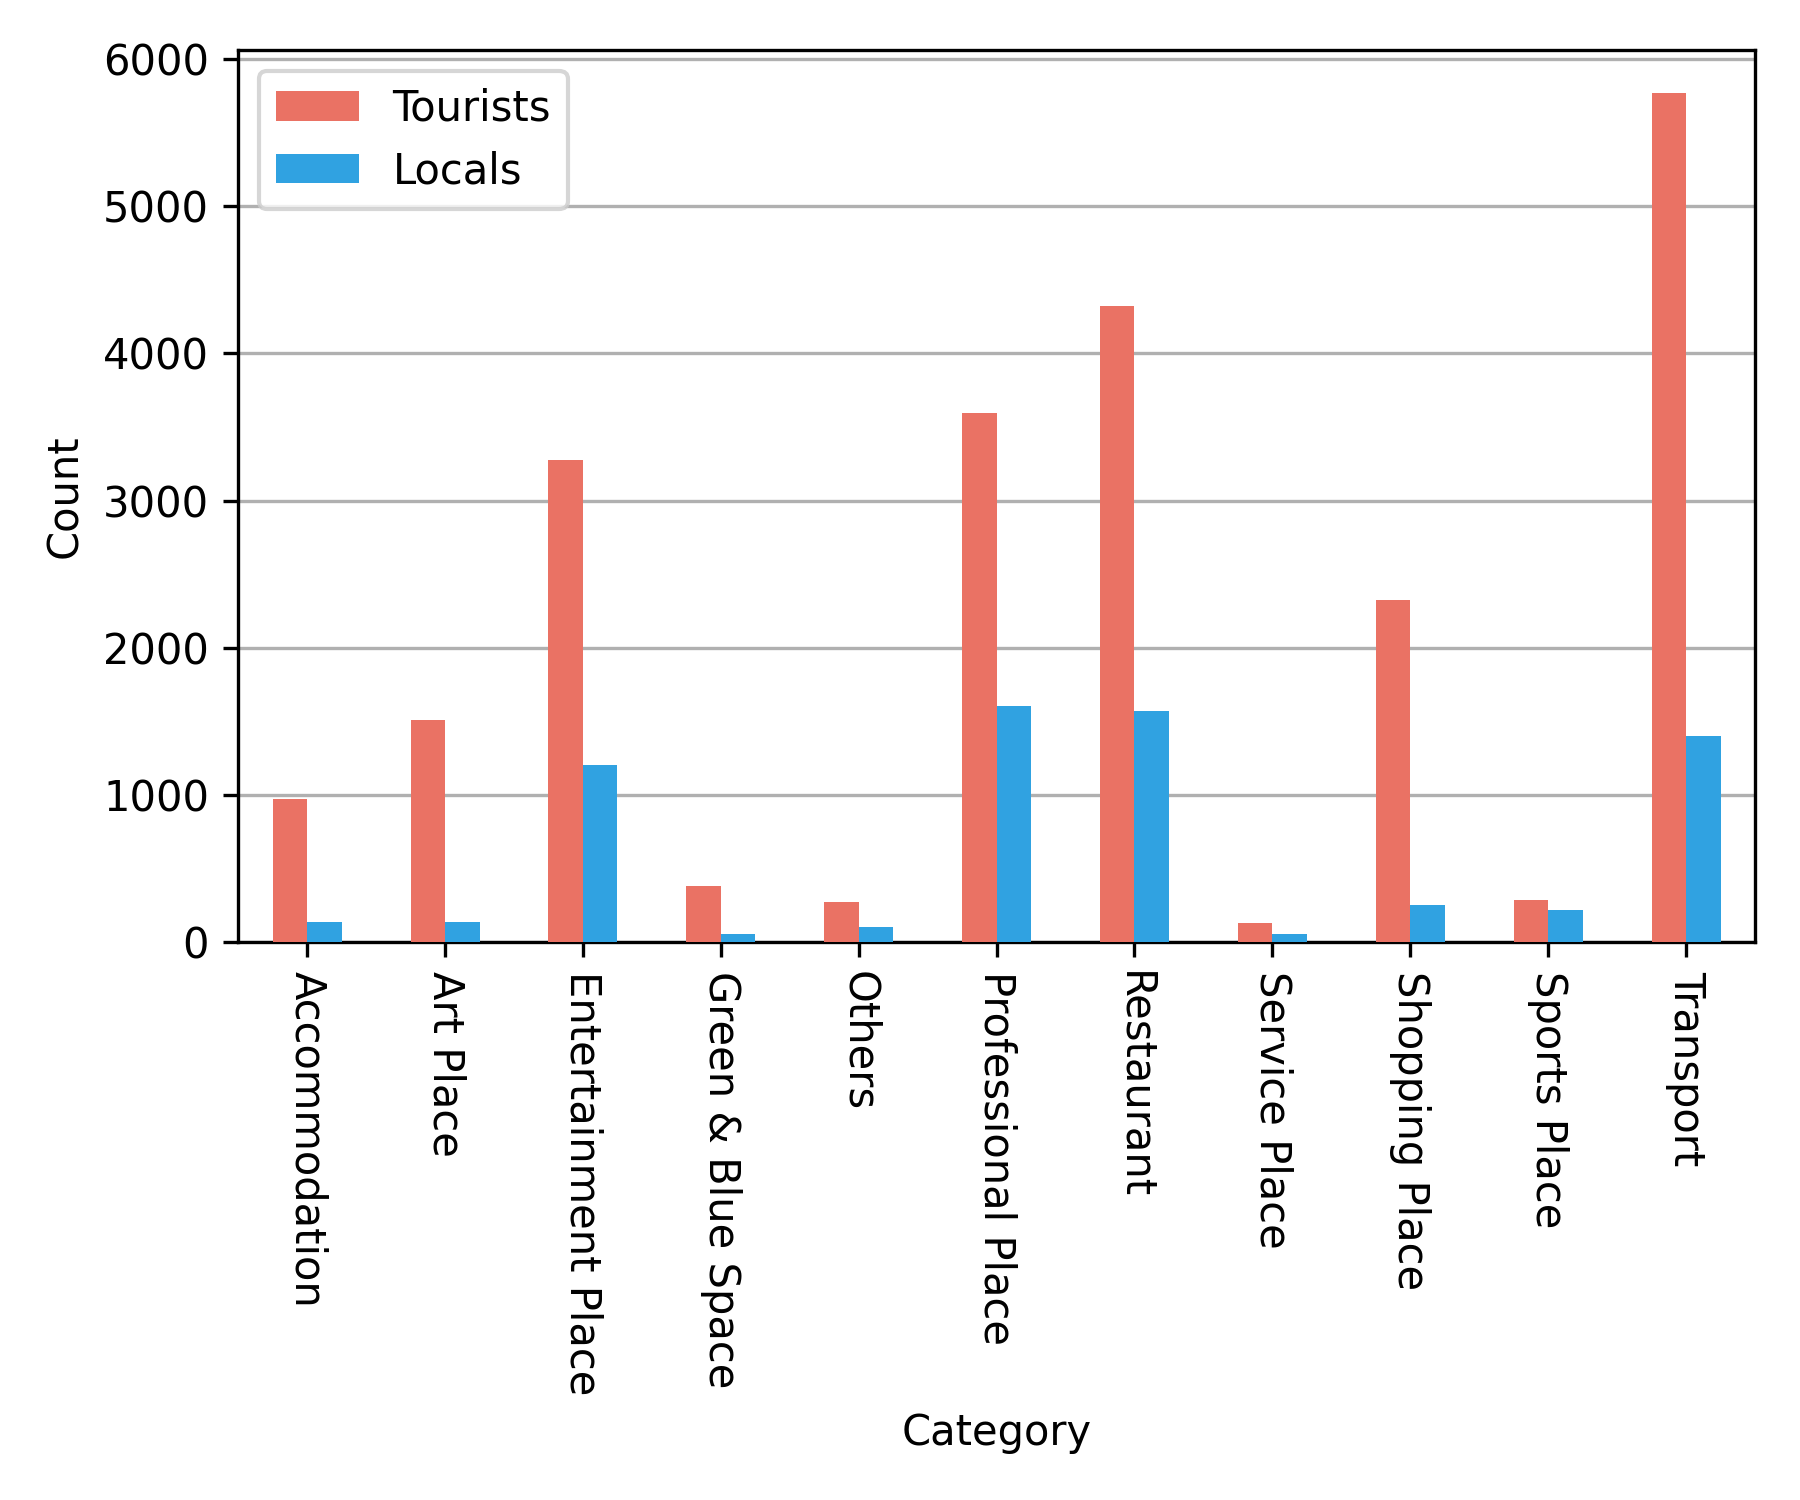
\includegraphics[width=1\linewidth]{figures/diff_pop_category_weekday.png} 
\caption{Weekday.}
\label{fig:diff_pop_category_weekday}
\end{subfigure}
\begin{subfigure}{0.5\textwidth}
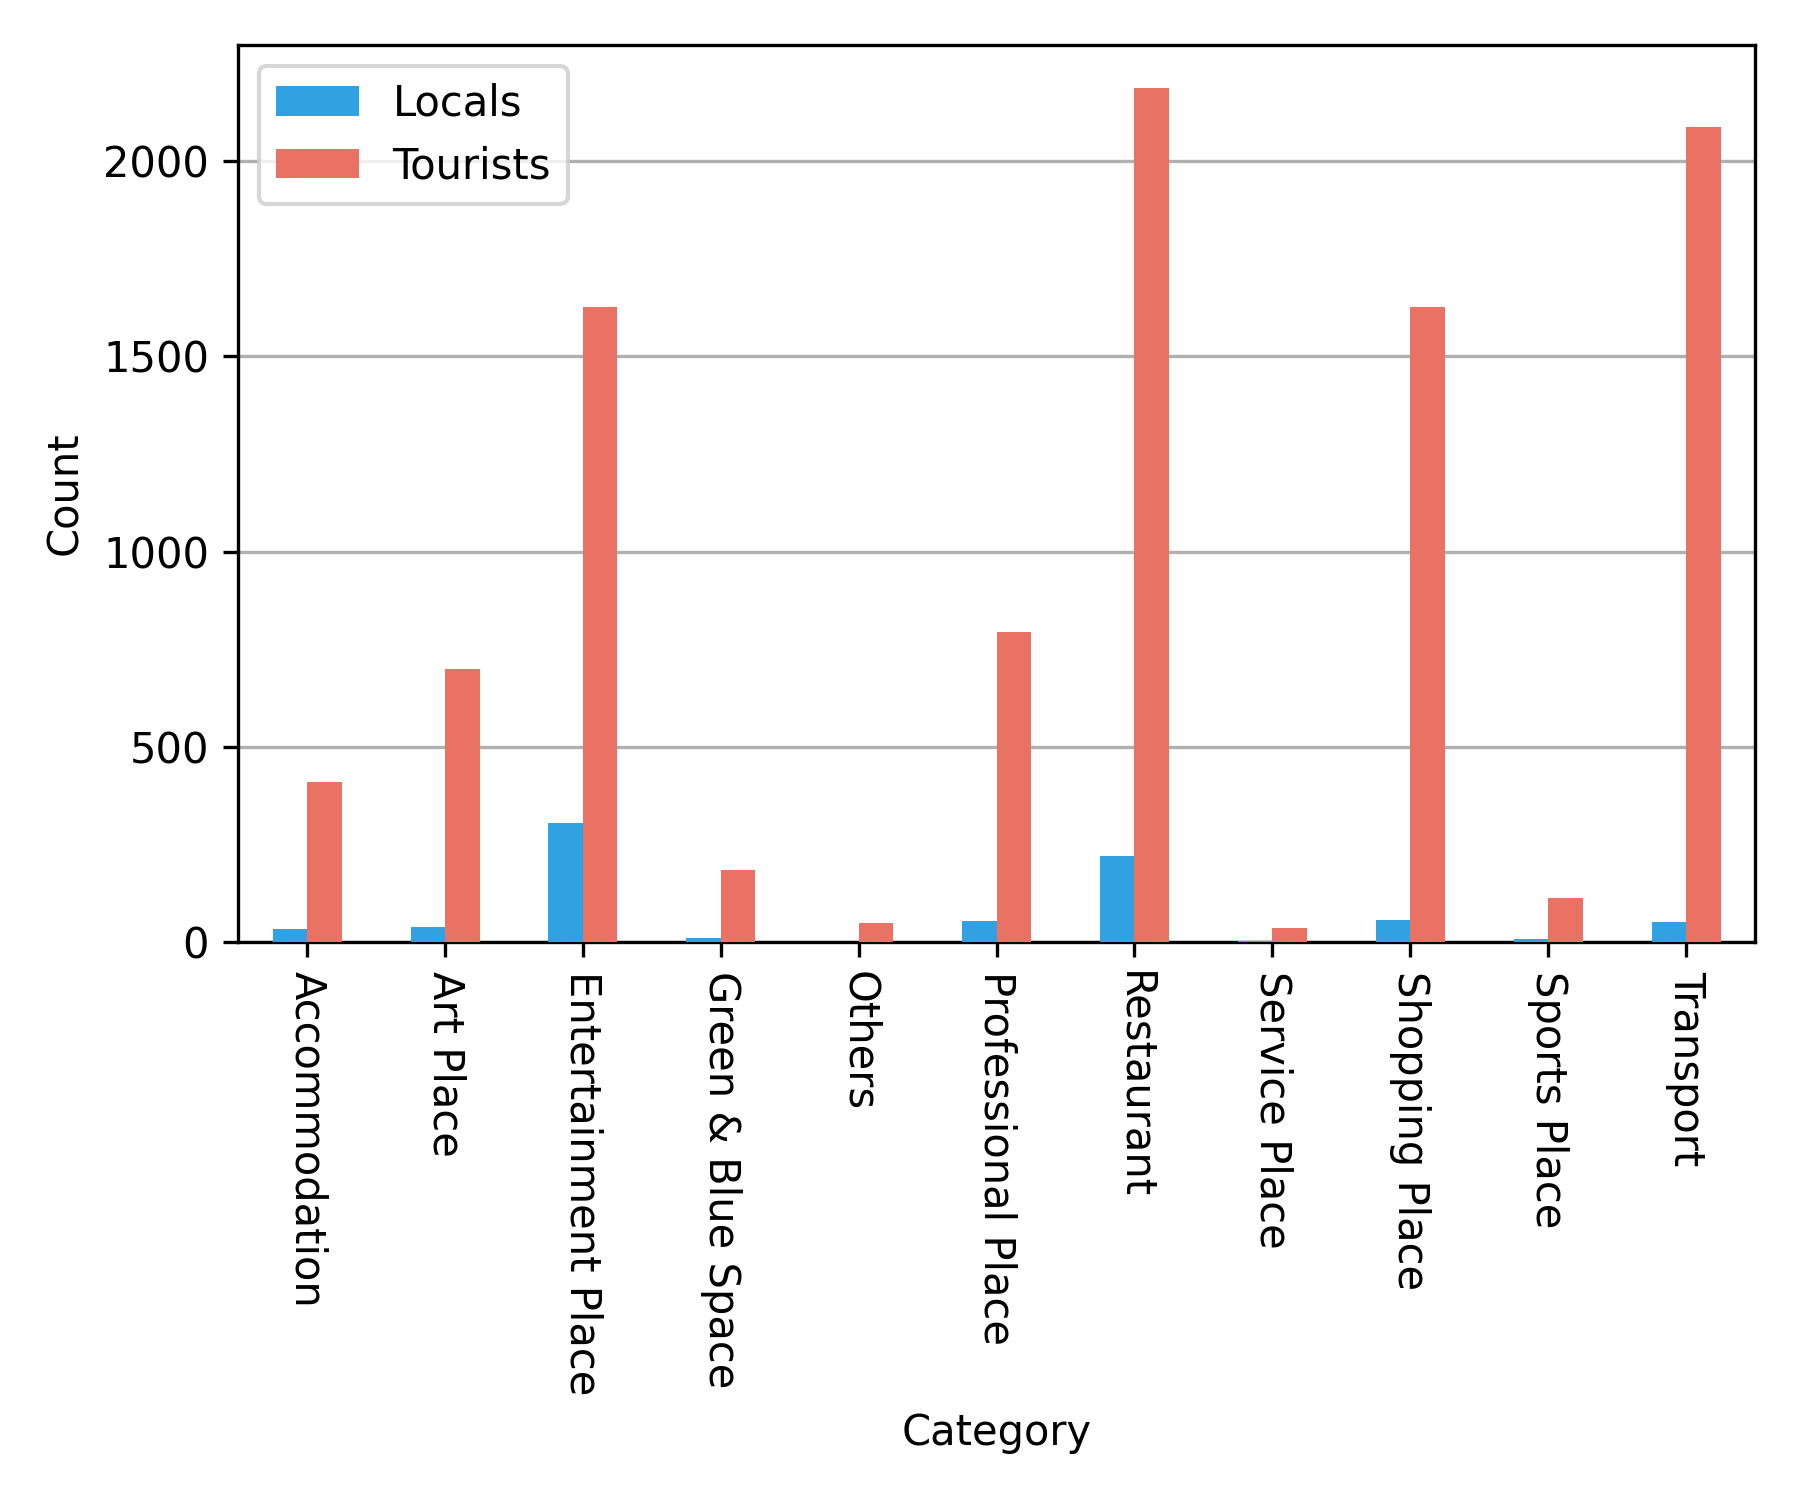
\includegraphics[width=1\linewidth]{figures/diff_pop_category_weekend.png}
\caption{Weekend.}
\label{fig:diff_pop_category_weekend}
\end{subfigure}

\caption{Number of check-in categories in popular areas on weekdays and weekends.} \label{fig:diff_pop_category_week}
\end{figure}


% ============================= || Spatiotemporal Patterns of Places || =============================
\subsection{Spatiotemporal Patterns of Places} \label{patterns_places}

% ====================== | Place Distribution | ======================
\subsubsection{Place Distribution}

\subsubsubsection{Daytime vs. Nighttime}
Places in this study refer to clusters of check-ins. Table~\ref{tab:places_summary} provides an overview of the number of places visited by locals and tourists at different time spans. It is worth noting that the removal of check-in outliers during the clustering process resulted in a reduced number of users. Although the number of tourists is considerably greater than that of locals, tourists tend to visit fewer places than locals. Figure~\ref{fig:places_distribution_day} displays the distribution of places throughout the day. During daytime hours, a total of 1,525 places are visited by locals. The majority of these places are concentrated in the city center, and there are also a certain number of places located in outskirts boroughs such as Hillingdon, Croydon, and Barnet. On the other hand, the 1,046 places visited by tourists exhibit a more concentrated distribution in the inner part of London, with a sparser distribution in the outer areas. During nighttime hours, the distribution of places follows a similar pattern to that of the daytime, but with a lower density. The number of places visited decreases to 598 by locals, and 441 by tourists, indicating a reduced activity level during nighttime hours.


\begin{table}[h!]
\centering
\caption{\label{tab:places_summary}Summary of places.}
\begin{tabular}{llll} \hline
Time & Population group & No. of users & No. of places \\
\hline
\multirow{3}{*}{Daytime} 
& All Users & 6,919 & 2,571 \\
& Locals & 1,077 & 1,525 \\
& Tourists & 5,842 & 1,046 \\
\hline
\multirow{3}{*}{Nighttime} 
& All Users & 4,425 & 1,039 \\
& Locals & 996 & 598 \\
& Tourists & 3,429 & 441 \\
\hline
\multirow{3}{*}{Weekday} 
& All Users & 6,497 & 2,524 \\
& Locals & 1,069 & 1,469 \\
& Tourists & 5,428 & 1,055 \\
\hline
\multirow{3}{*}{Weekend} 
& All Users & 4,886 & 1,435 \\
& Locals & 1,011 & 855 \\
& Tourists & 3,875 & 580 \\
\hline
\end{tabular}
\end{table}


\begin{figure}[!h]

\centering
\begin{subfigure}{0.6\textheight}
\centering
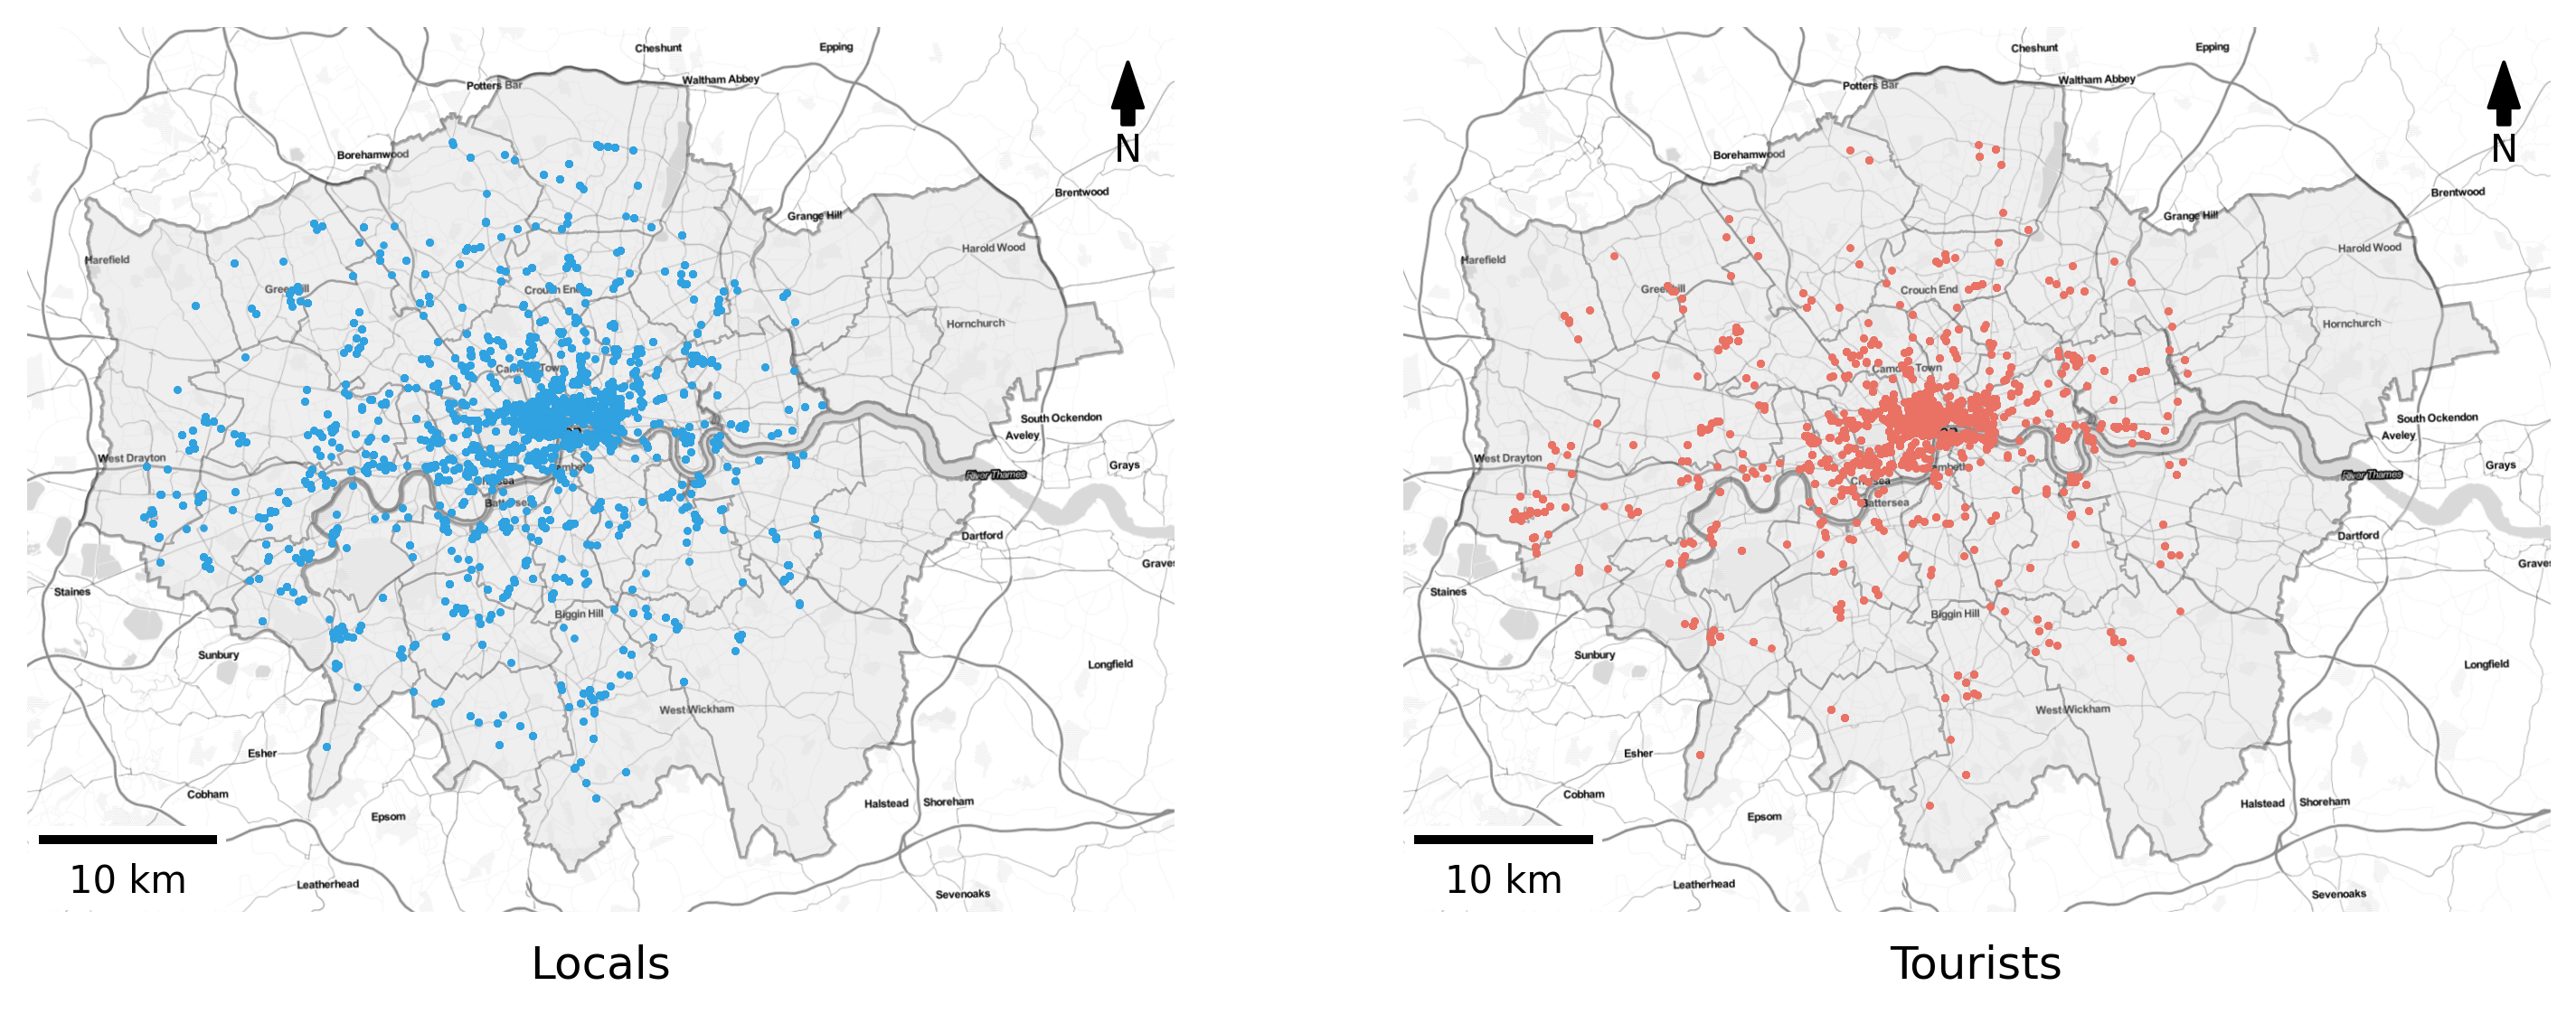
\includegraphics[width=0.9\linewidth]{figures/places_daytime.png} 
\caption{Daytime.}
\label{fig:places_daytime}
\end{subfigure}
\begin{subfigure}{0.6\textheight}
\centering
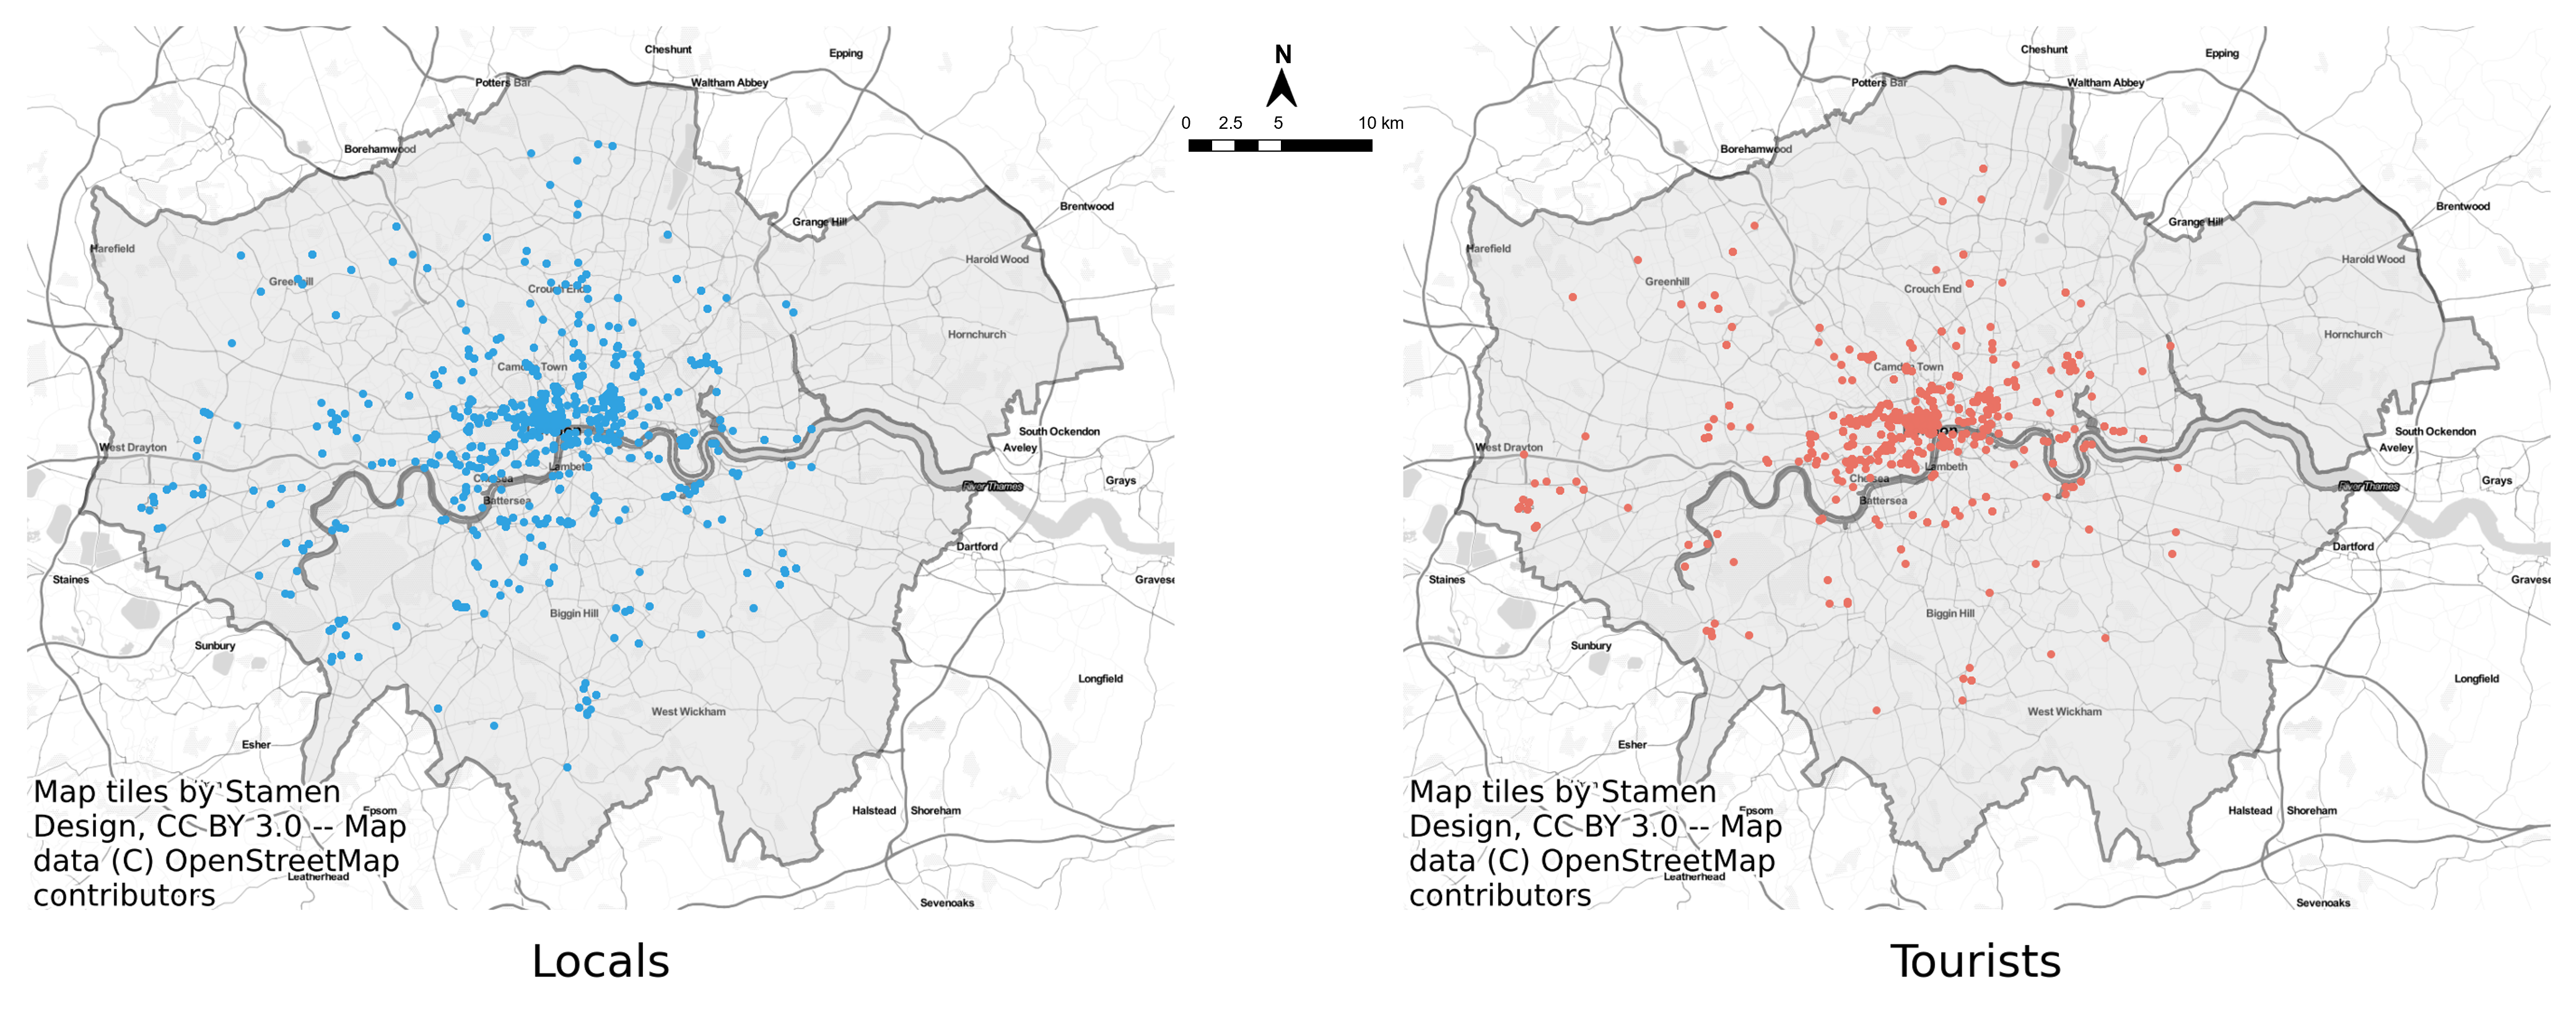
\includegraphics[width=0.9\linewidth]{figures/places_nighttime.png}
\caption{Nighttime.}
\label{fig:places_nighttime}
\end{subfigure}

\caption{Distribution of places during the daytime and nighttime.}
\label{fig:places_distribution_day}
\end{figure}


\subsubsubsection{Weekday vs. Weekend}
Figure~\ref{fig:places_distribution_week} showcases the distribution of places on weekdays and weekends. On weekdays, both locals and tourists visit a significant number of places in the city center, but locals tend to visit more places in suburban areas compared to tourists. Specifically, locals visit 1,469 places, whereas tourists visit 1,055 places. On weekends, the distributions of places for locals and tourists become sparser compared to weekdays, but the concentration in the city center remains evident. Similar to weekdays, locals continue to visit more places on the outskirts of London than tourists. Overall, both locals and tourists tend to concentrate in the city center but also exhibit distinct distribution patterns of places across time spans.


\begin{figure}[!h]

\centering
\begin{subfigure}{0.6\textheight}
\centering
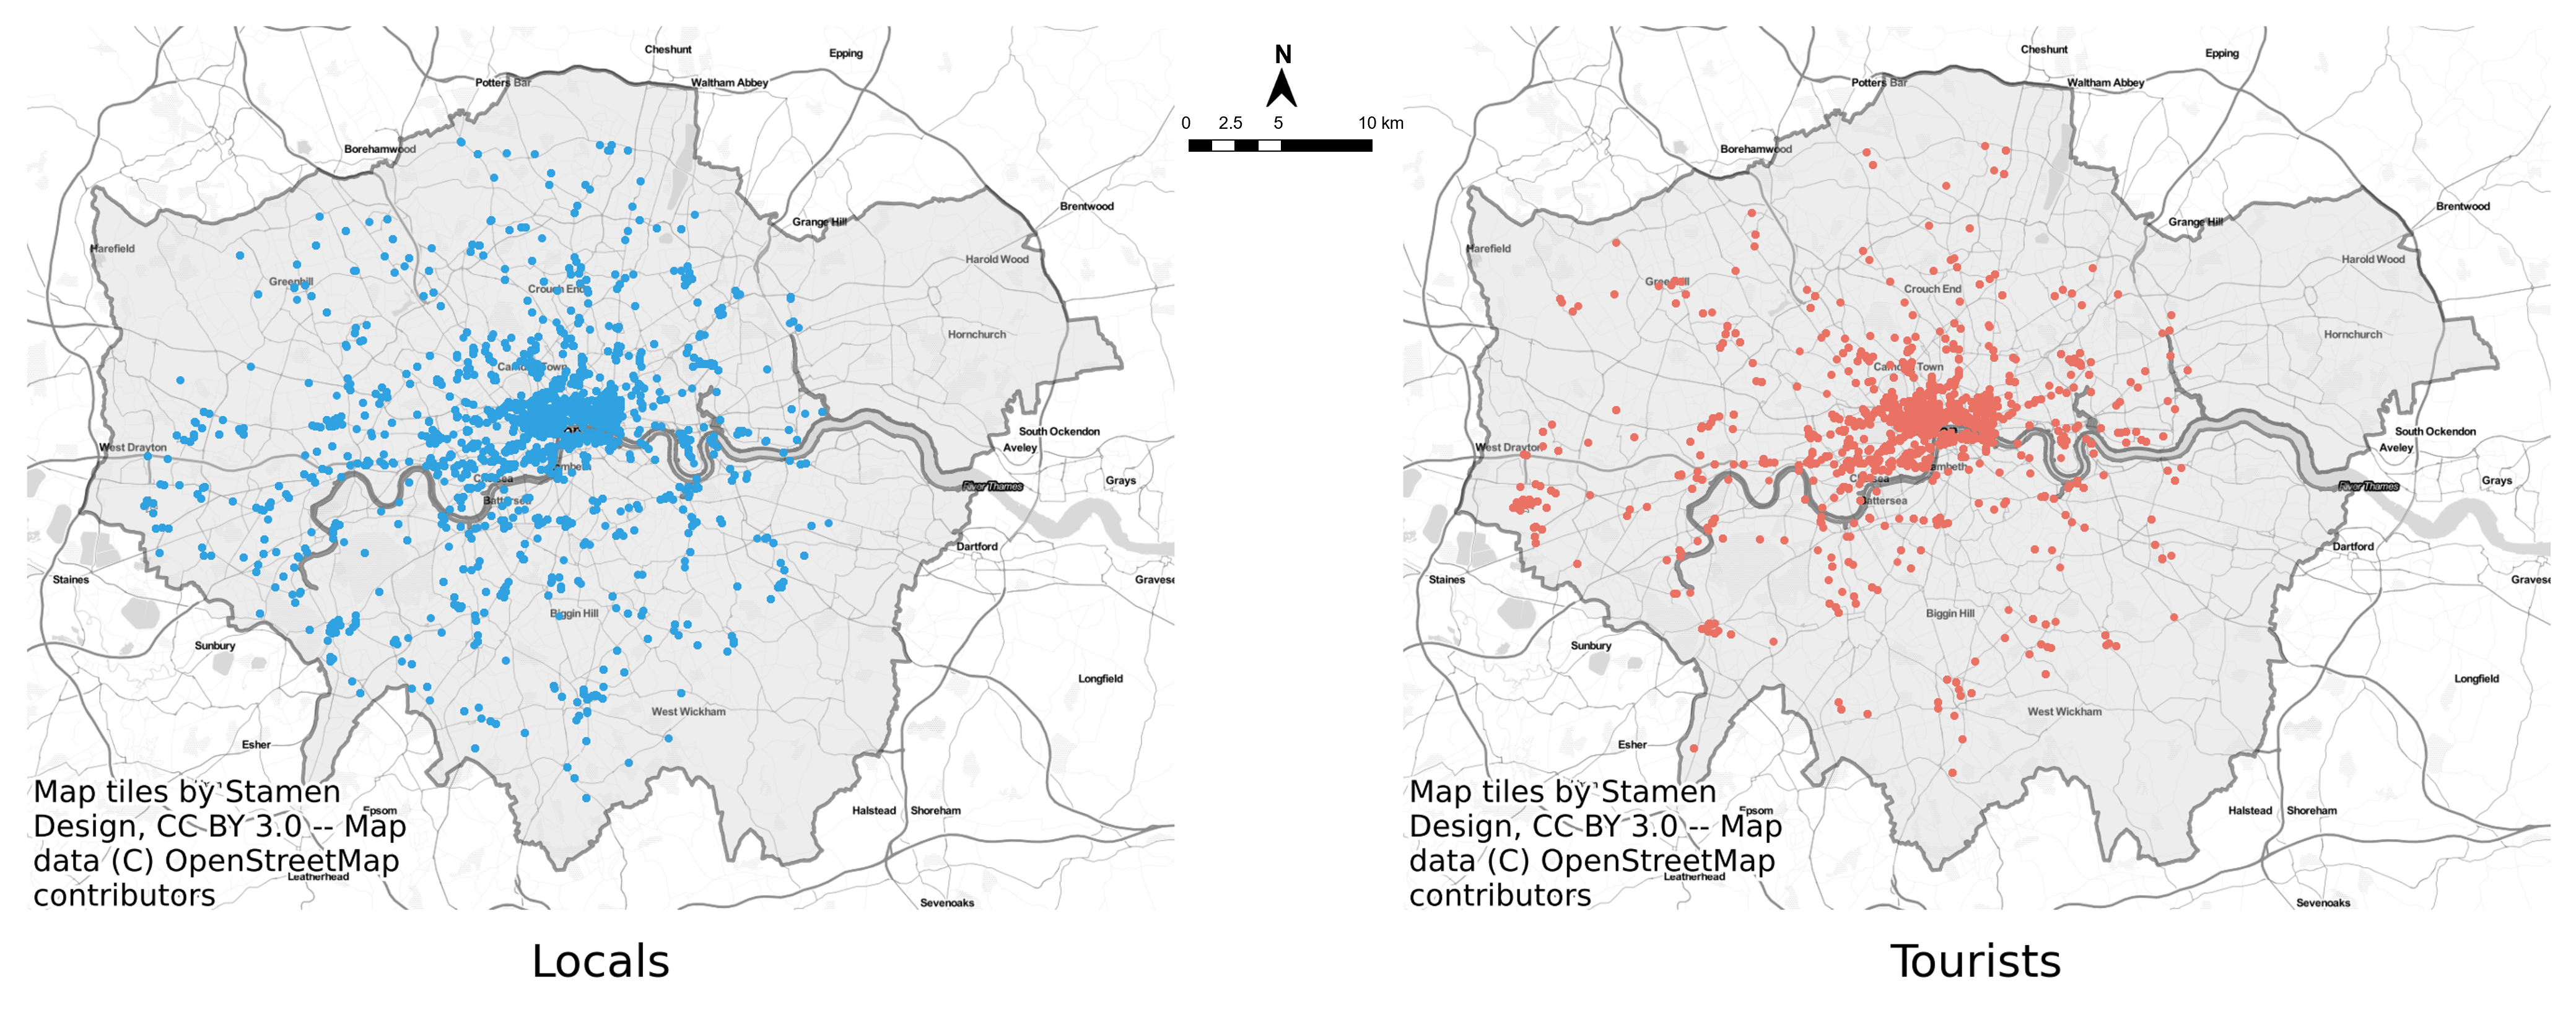
\includegraphics[width=0.9\linewidth]{figures/places_weekday.png}
\caption{Weekday.}
\label{fig:places_weekday}
\end{subfigure}
\begin{subfigure}{0.6\textheight}
\centering
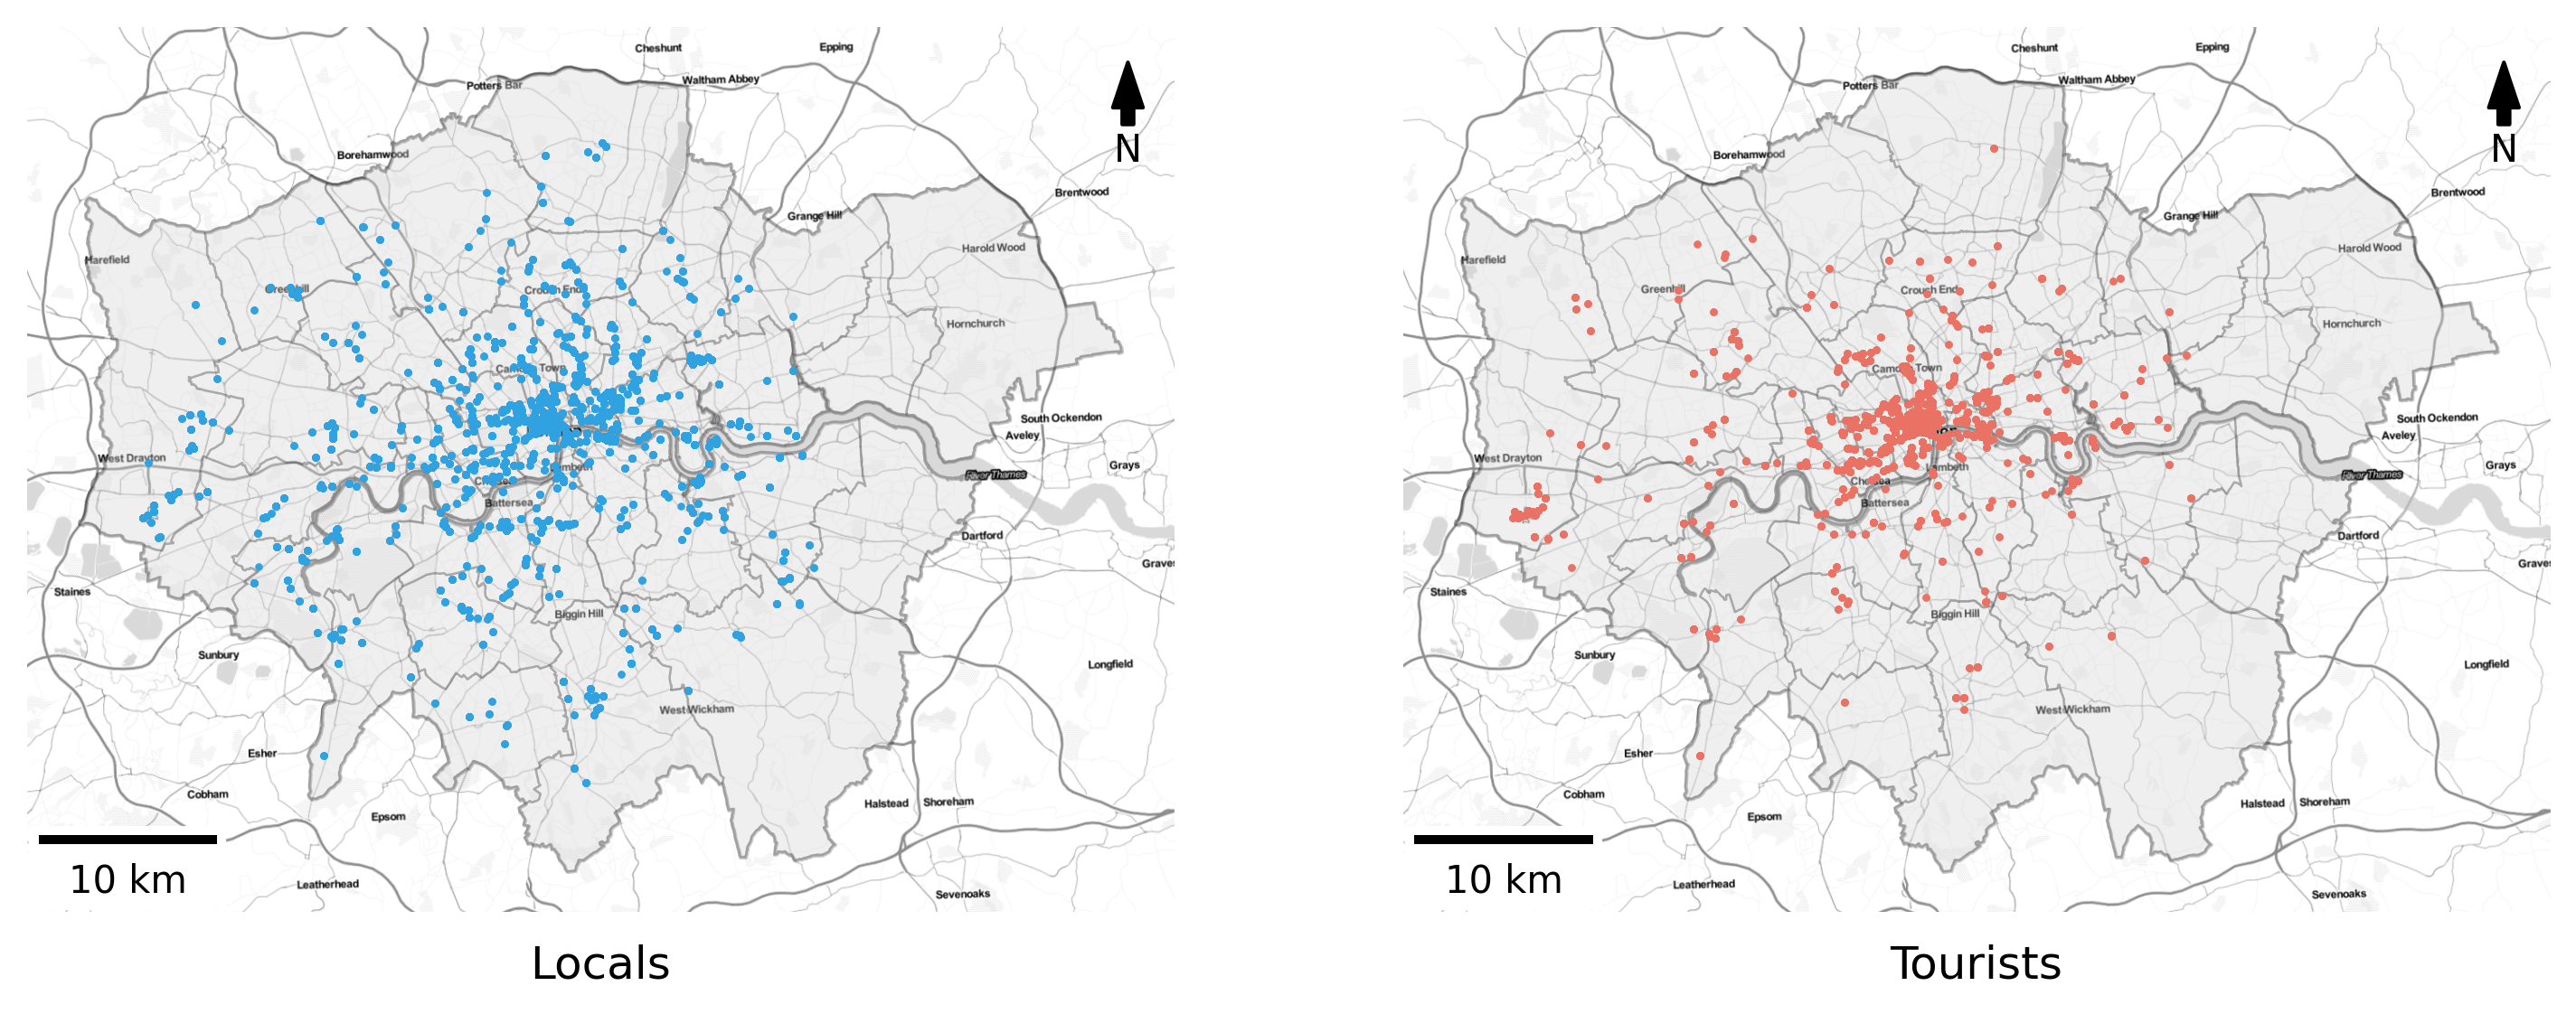
\includegraphics[width=0.9\linewidth]{figures/places_weekend.png}
\caption{Weekend.}
\label{fig:places_weekend}
\end{subfigure}

\caption{Distribution of places on weekdays and weekends.}
\label{fig:places_distribution_week}
\end{figure}



% ====================== | Place Dimensions | ======================
\subsubsection{Place Dimensions}

% ============== Daytime vs. Nighttime ==============
\subsubsubsection{Daytime vs. Nighttime}

\textbf{Location}

Figure~\ref{fig:places_location_day} provides insight into the distribution of places in the \textit{Location} dimension during the daytime and nighttime. The central boroughs of Westminster and Camden contain the highest number of places visited by both locals and tourists throughout the day, which also validates the findings in the previous section. Figure~\ref{fig:places_location_daytime} shows that during the daytime, most outskirts boroughs have more places visited by locals rather than tourists. This trend is obvious in boroughs such as Barnet, Islington, Harrow, and Merton, as these outer areas serve as residential settlements. It is worth mentioning that Hillingdon, also an outer borough, exhibits a higher number of places visited by tourists, which can be attributed to the presence of Heathrow Airport in its southern region. Boroughs with a relatively equal number of places visited by locals and tourists are predominantly located in the inner part of London. These boroughs include Westminster, Camden, the City of London, Kensington and Chelsea, and Tower Hamlets, all of which boast a higher concentration of tourist attractions with high accessibility. Figure~\ref{fig:places_location_nighttime} illustrates the \textit{Location} dimension of places during the nighttime. While the overall number of places visited decreases in all boroughs during night hours, the distribution remains similar to that of the daytime.


\begin{figure}[!h]

\centering
\begin{subfigure}{0.6\textheight}
\centering
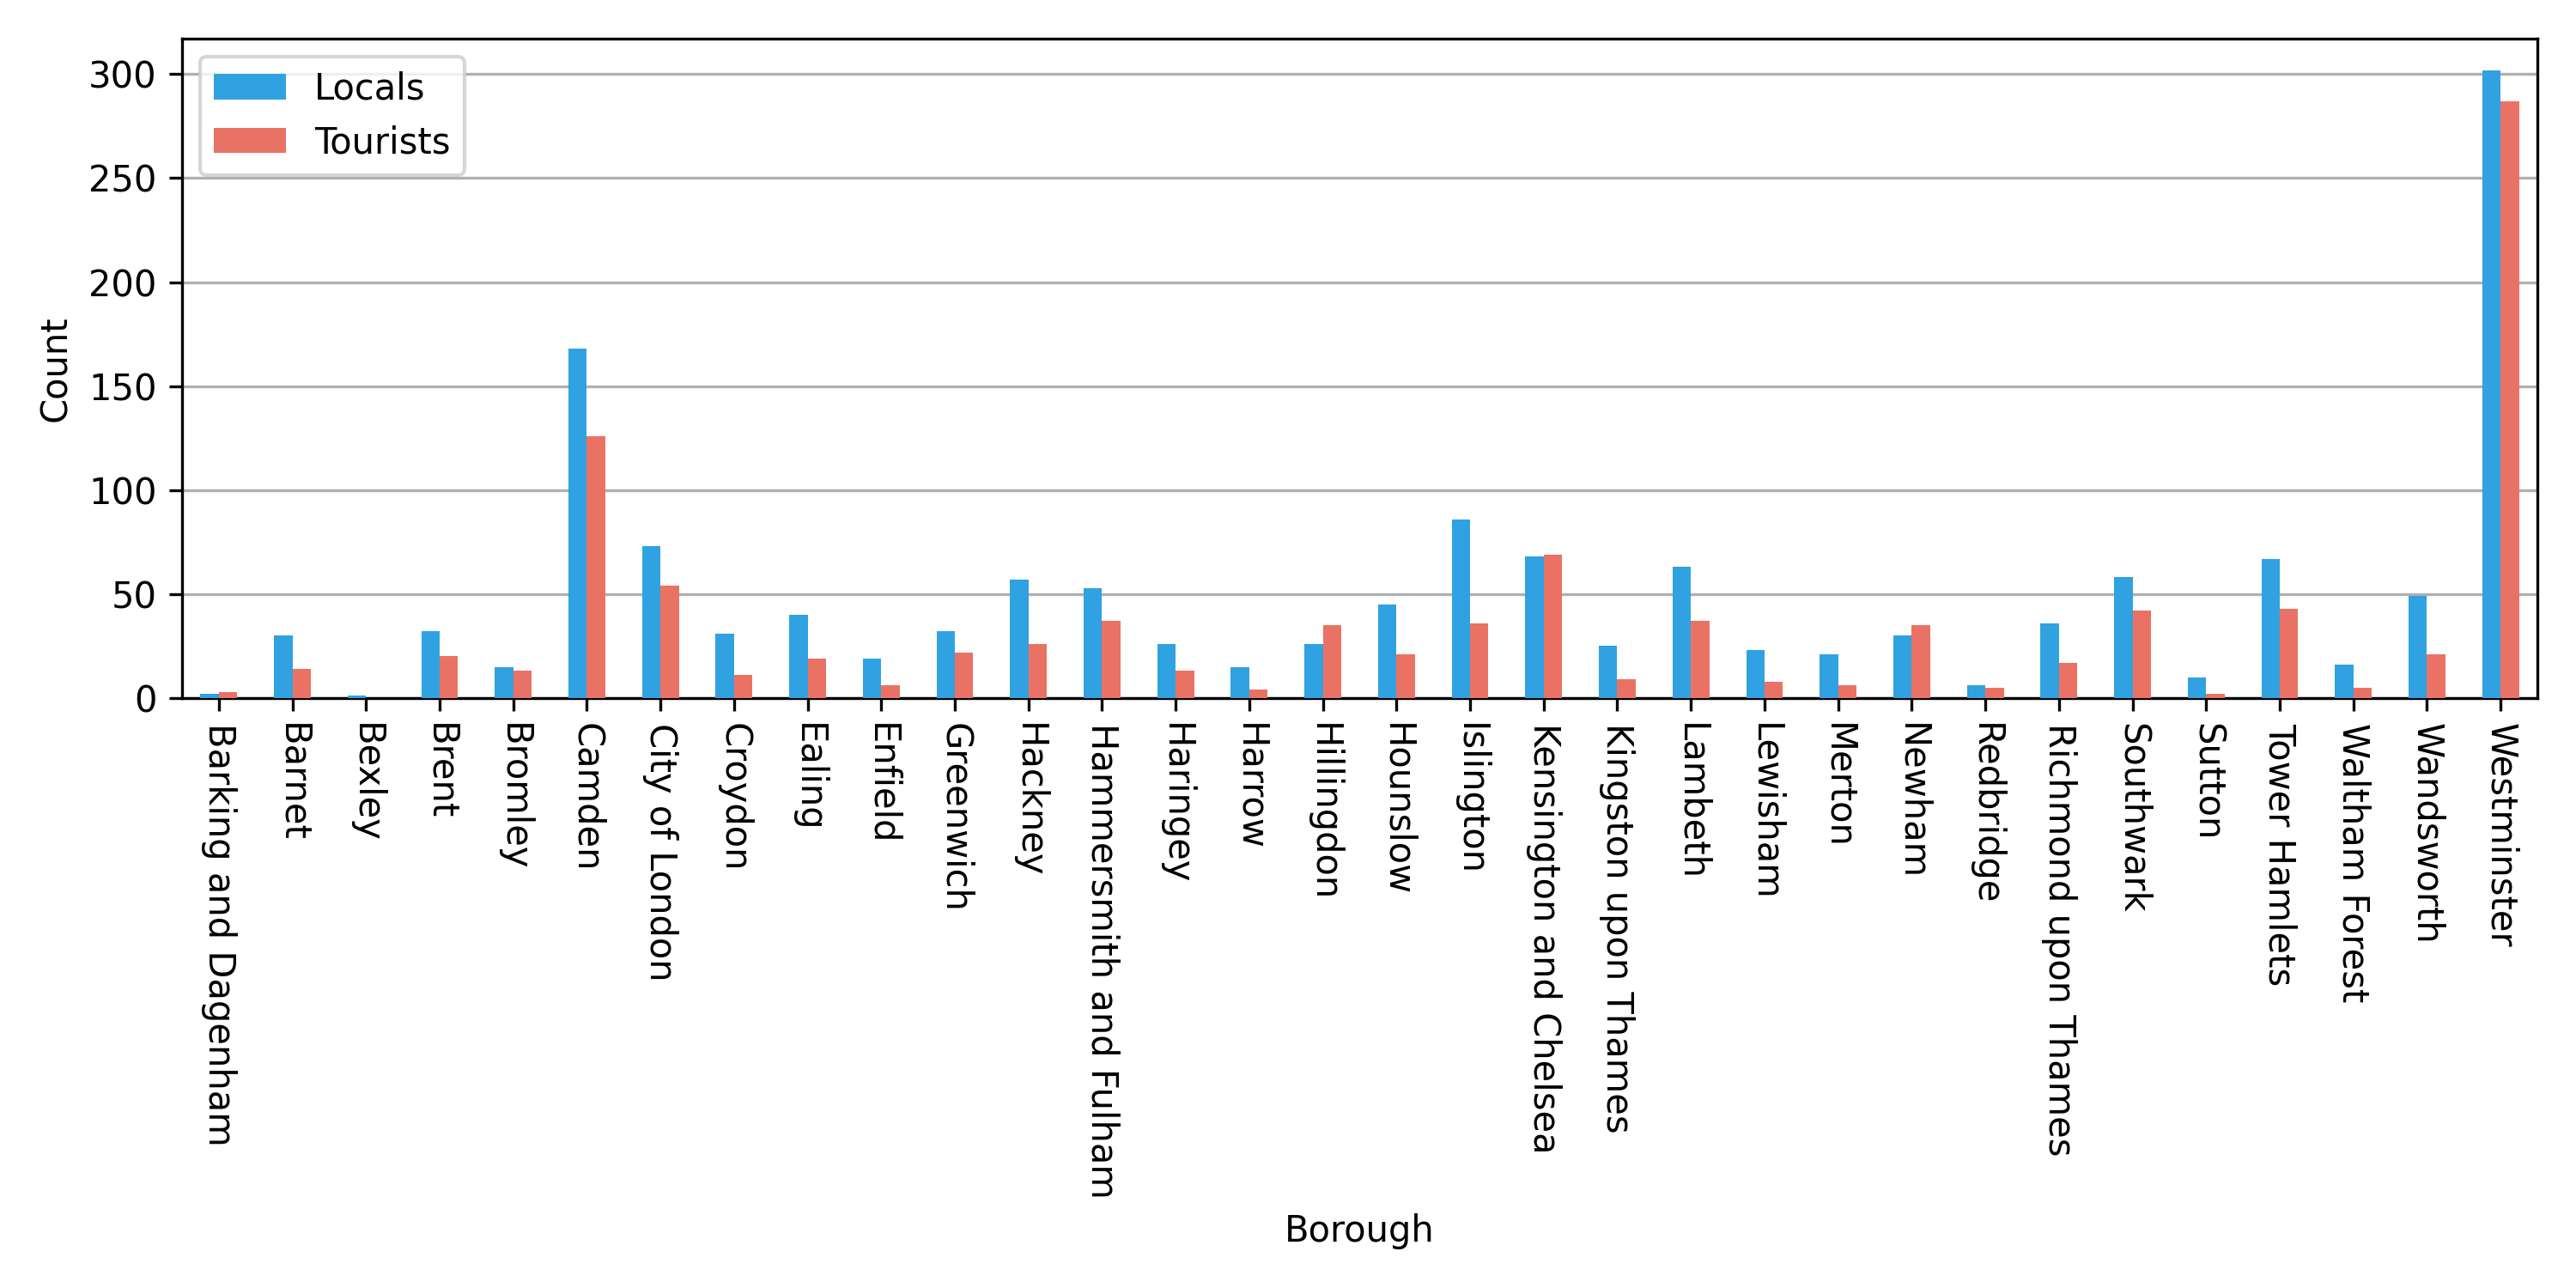
\includegraphics[width=0.9\linewidth]{figures/places_location_daytime.png} 
\caption{Daytime.}
\label{fig:places_location_daytime}
\end{subfigure}
\begin{subfigure}{0.6\textheight}
\centering
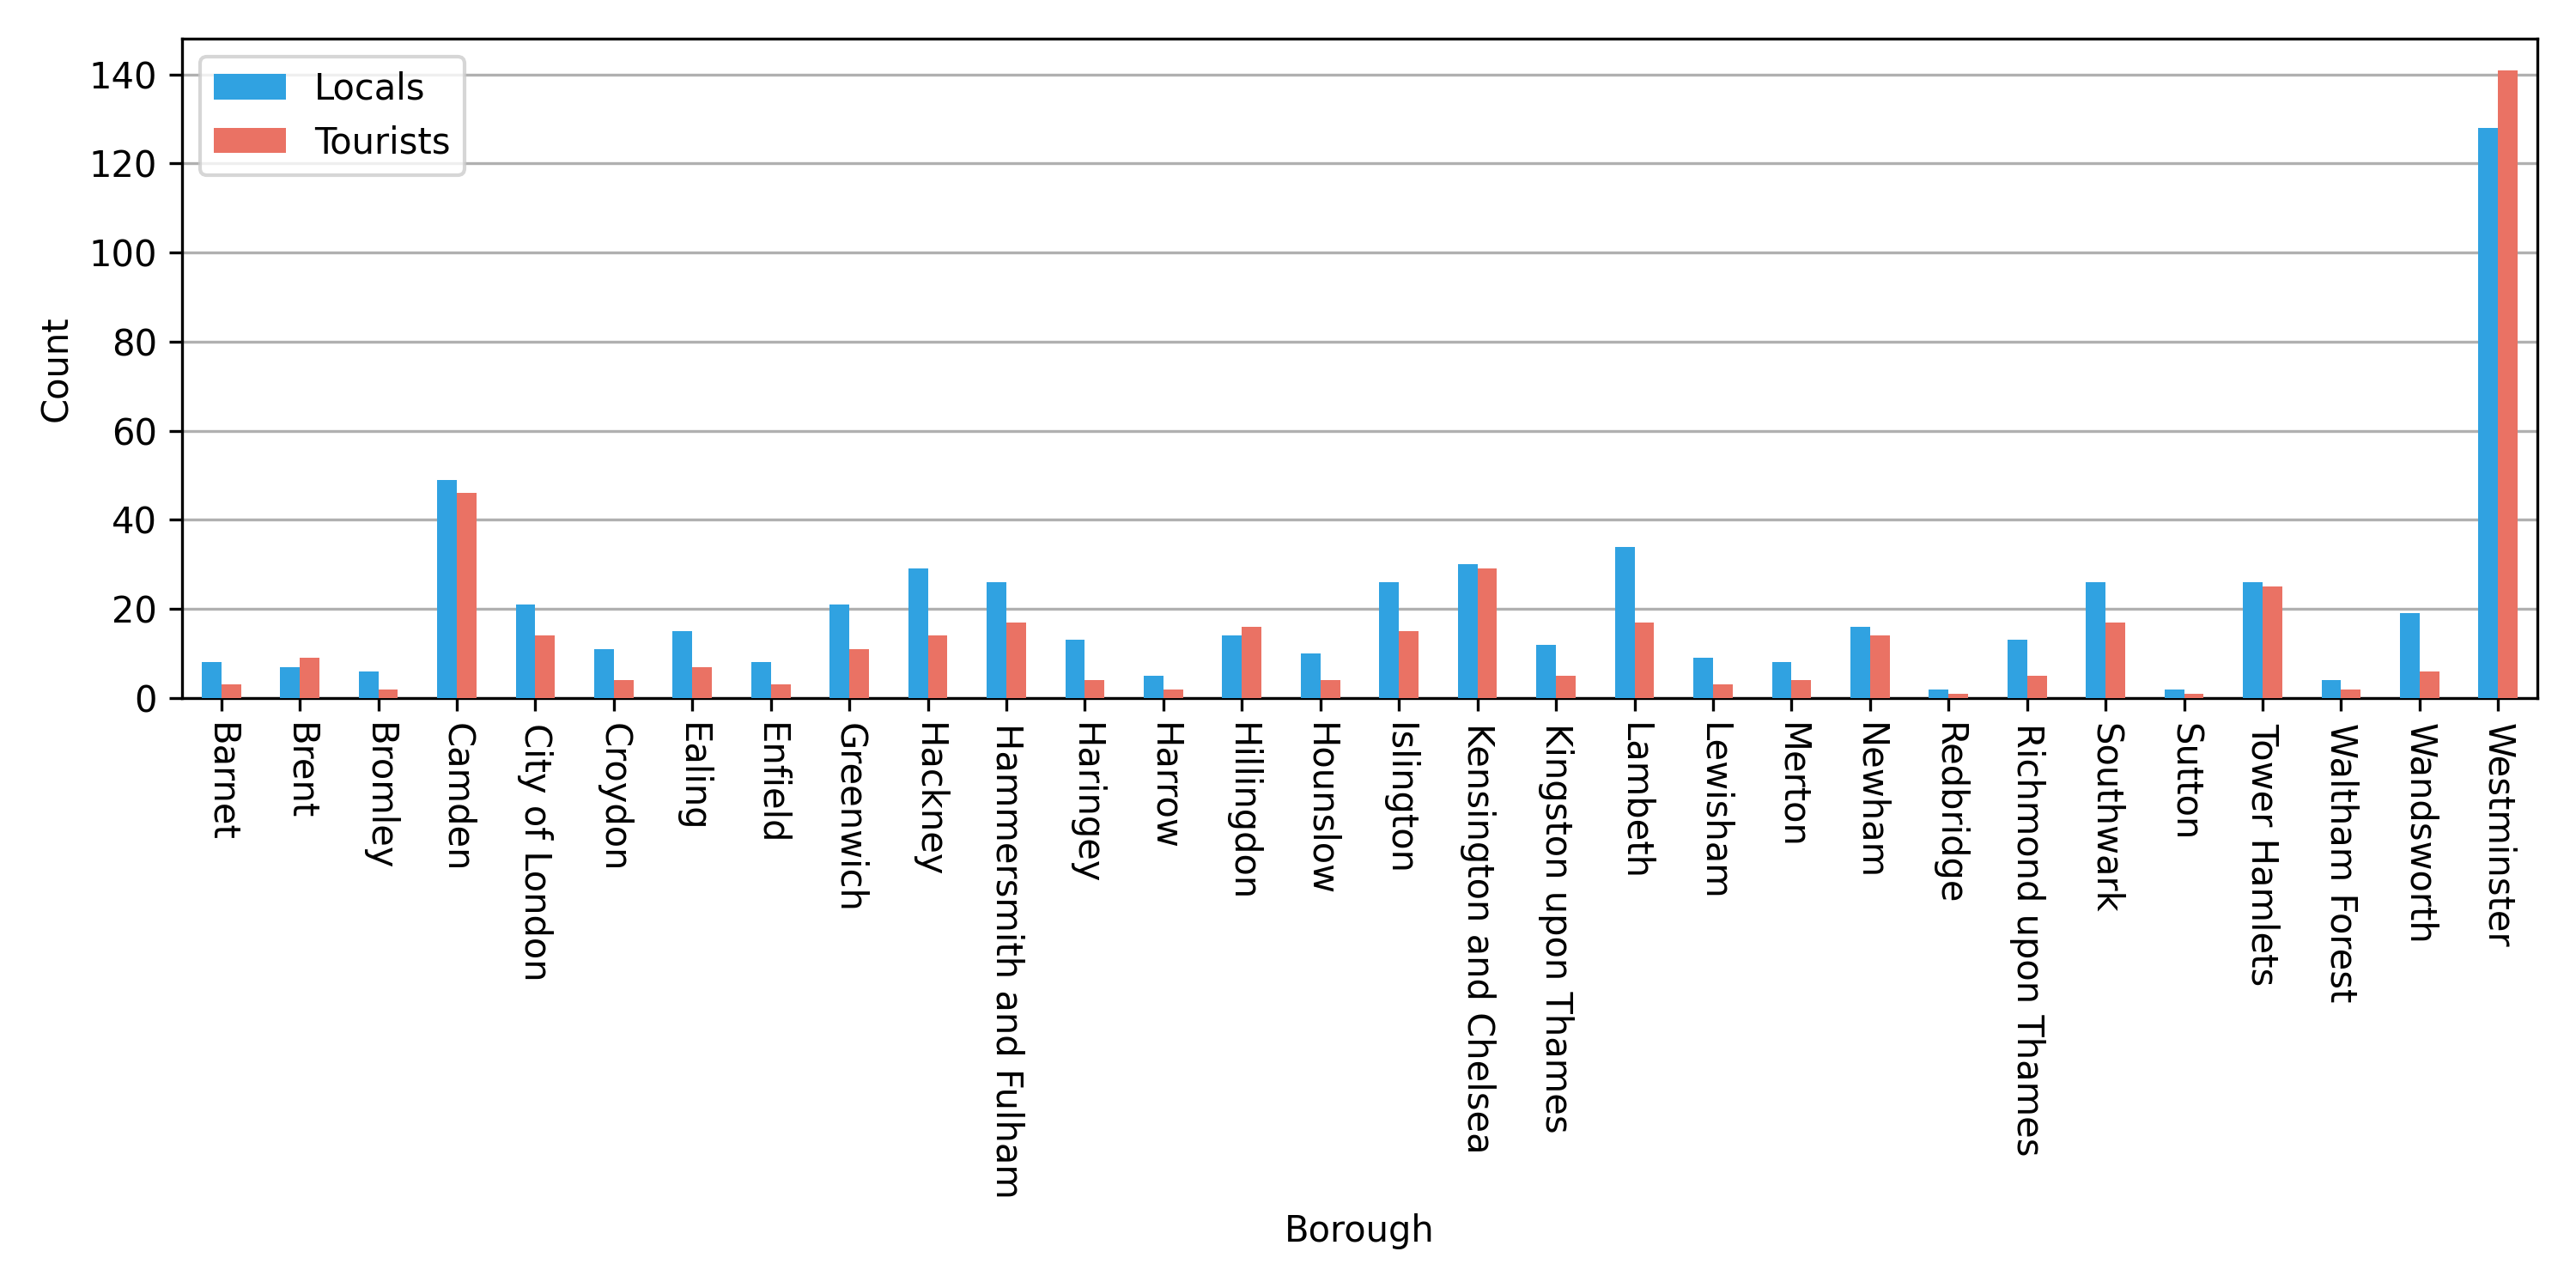
\includegraphics[width=0.9\linewidth]{figures/places_location_nighttime.png}
\caption{Nighttime.}
\label{fig:places_location_nighttime}
\end{subfigure}

\caption{Location dimension of places during the daytime and nighttime.}
\label{fig:places_location_day}
\end{figure}


\textbf{Locale}

Figure~\ref{fig:places_locale_day} shows the distribution of places in the \textit{Locale} dimension throughout the day. During daytime hours, restaurants are the most frequently visited categories for locals and tourists, and categories like professional places, shopping places, entertainment places, and transportation places are also popular among these two groups of people. Locals visit more places across most categories, but tourists show a higher preference for accommodation and green \& blue space categories than locals. At nighttime, fewer places are visited in each category and the popularity of these categories also undergoes a transformation. Restaurants remain its high popularity among both locals and tourists, and entertainment places emerge as the second most popular category, while there is a noticeable decrease in the frequency of professional places and shopping places compared to daytime hours. Accommodation and green \& blue spaces continue to attract more tourists than locals during nighttime hours. Notably, the accommodation category experiences an increased difference between the number of places visited by locals and tourists, indicating a higher demand for accommodation among tourists than locals during the nighttime.


\begin{figure}[!h]

\centering
\begin{subfigure}{0.6\textheight}
\centering
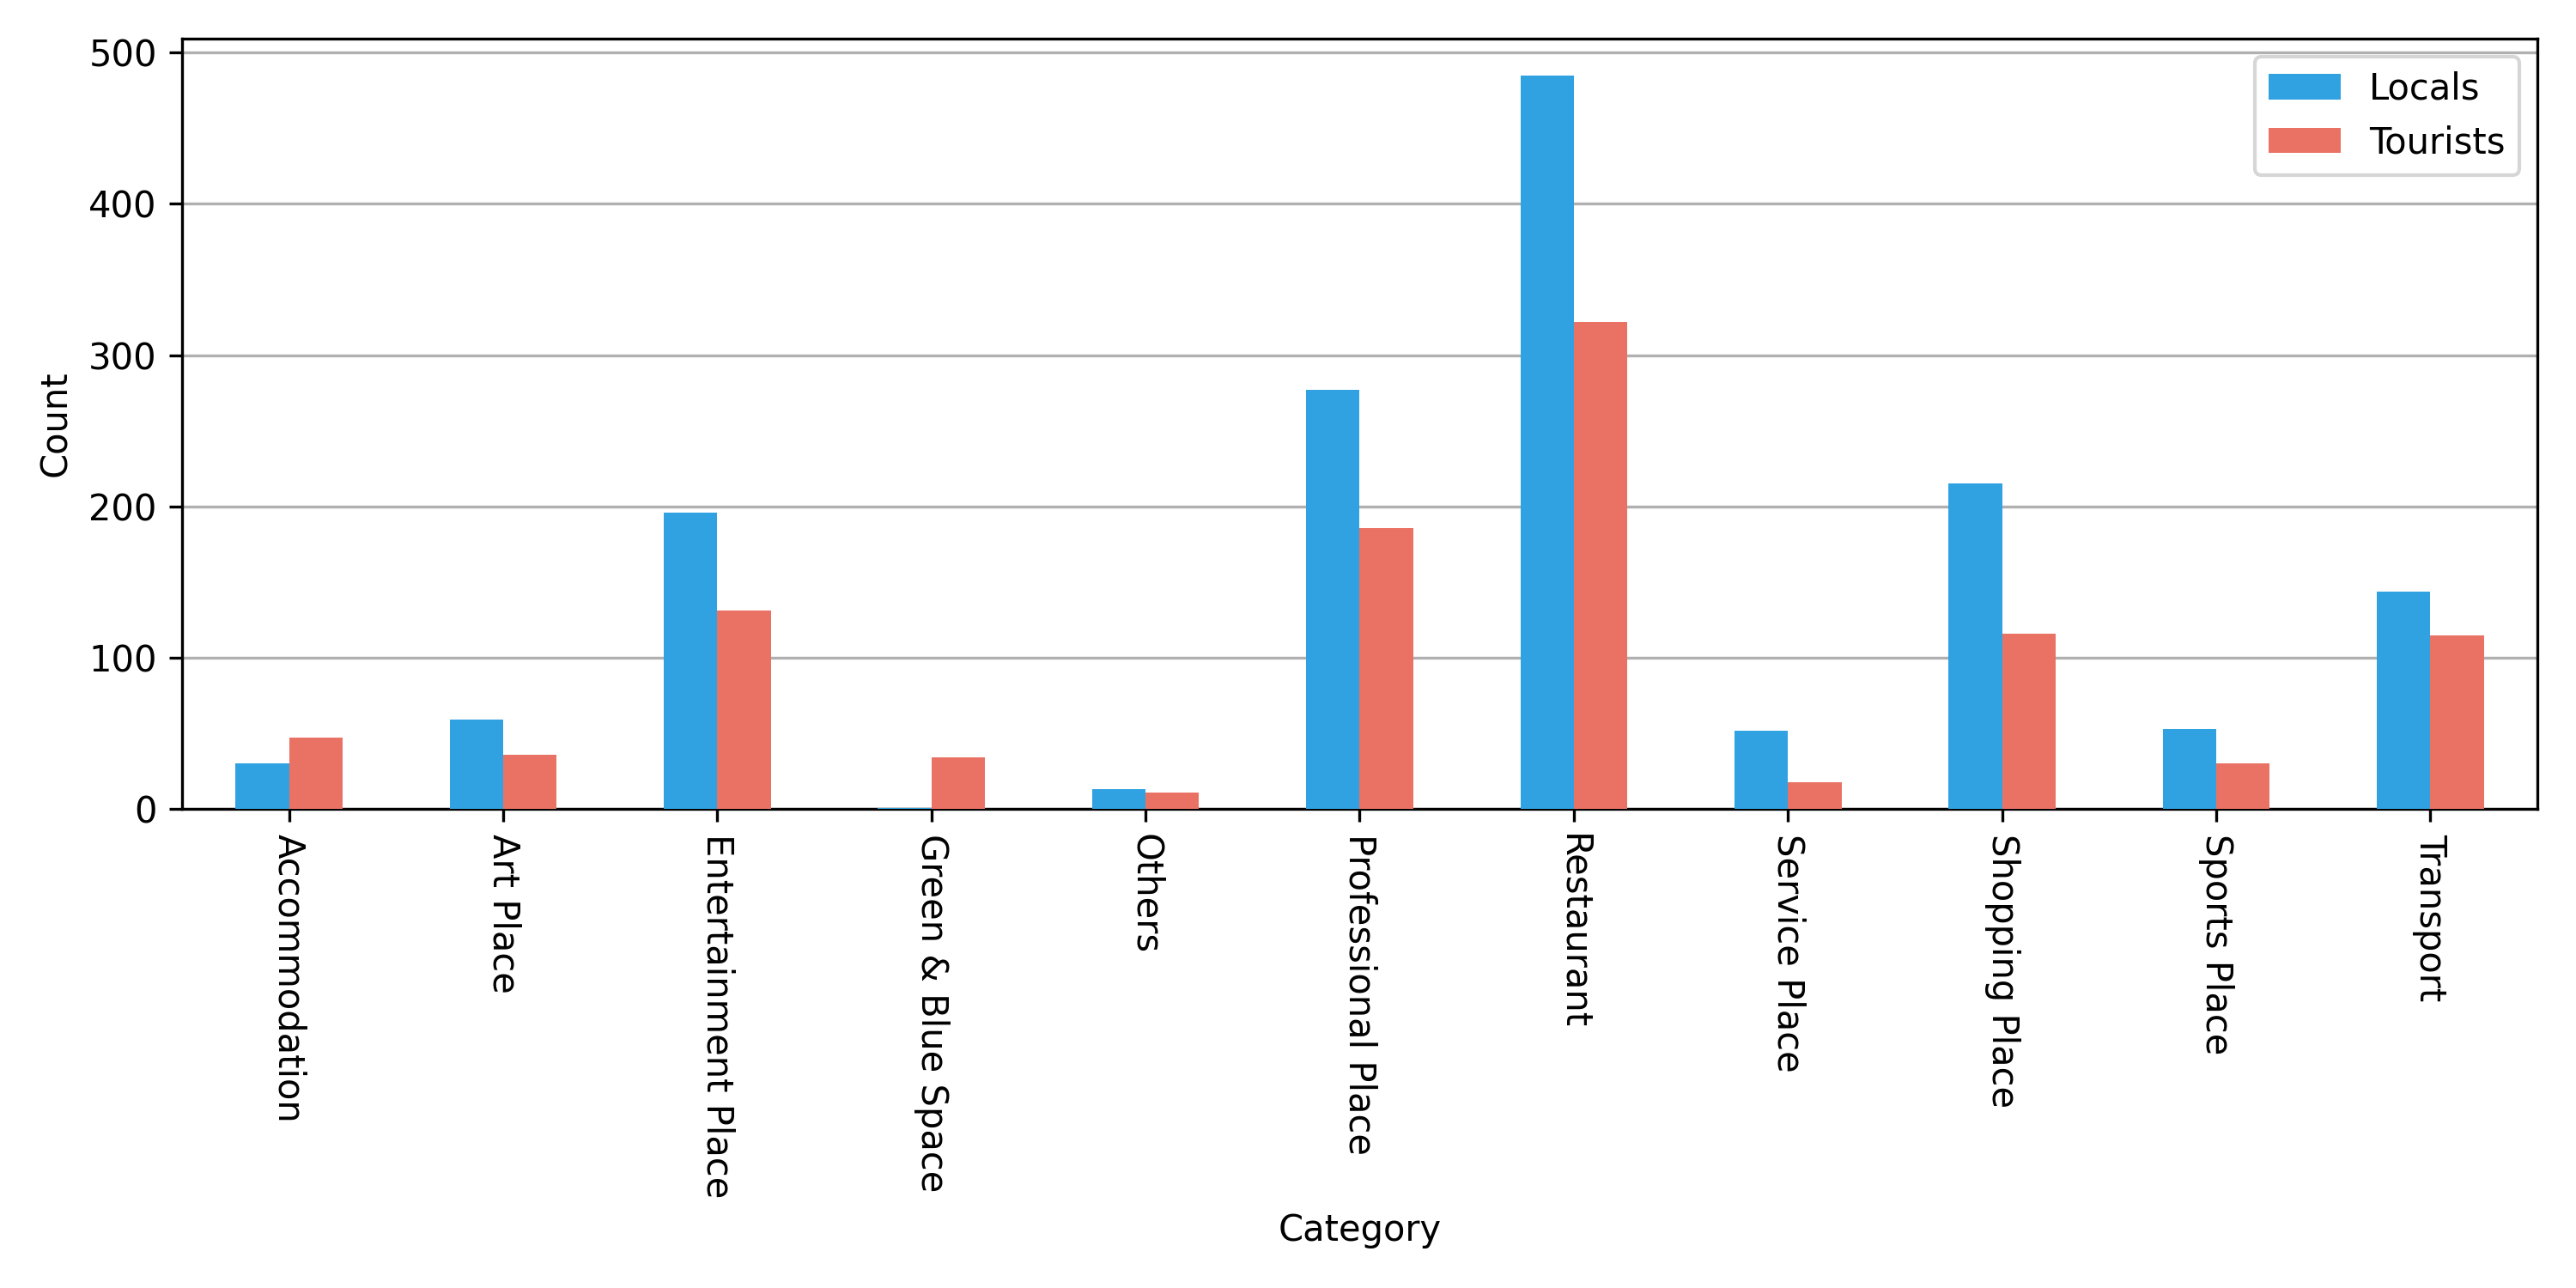
\includegraphics[width=0.9\linewidth]{figures/places_locale_daytime.png} 
\caption{Daytime.}
\label{fig:places_locale_daytime}
\end{subfigure}
\begin{subfigure}{0.6\textheight}
\centering
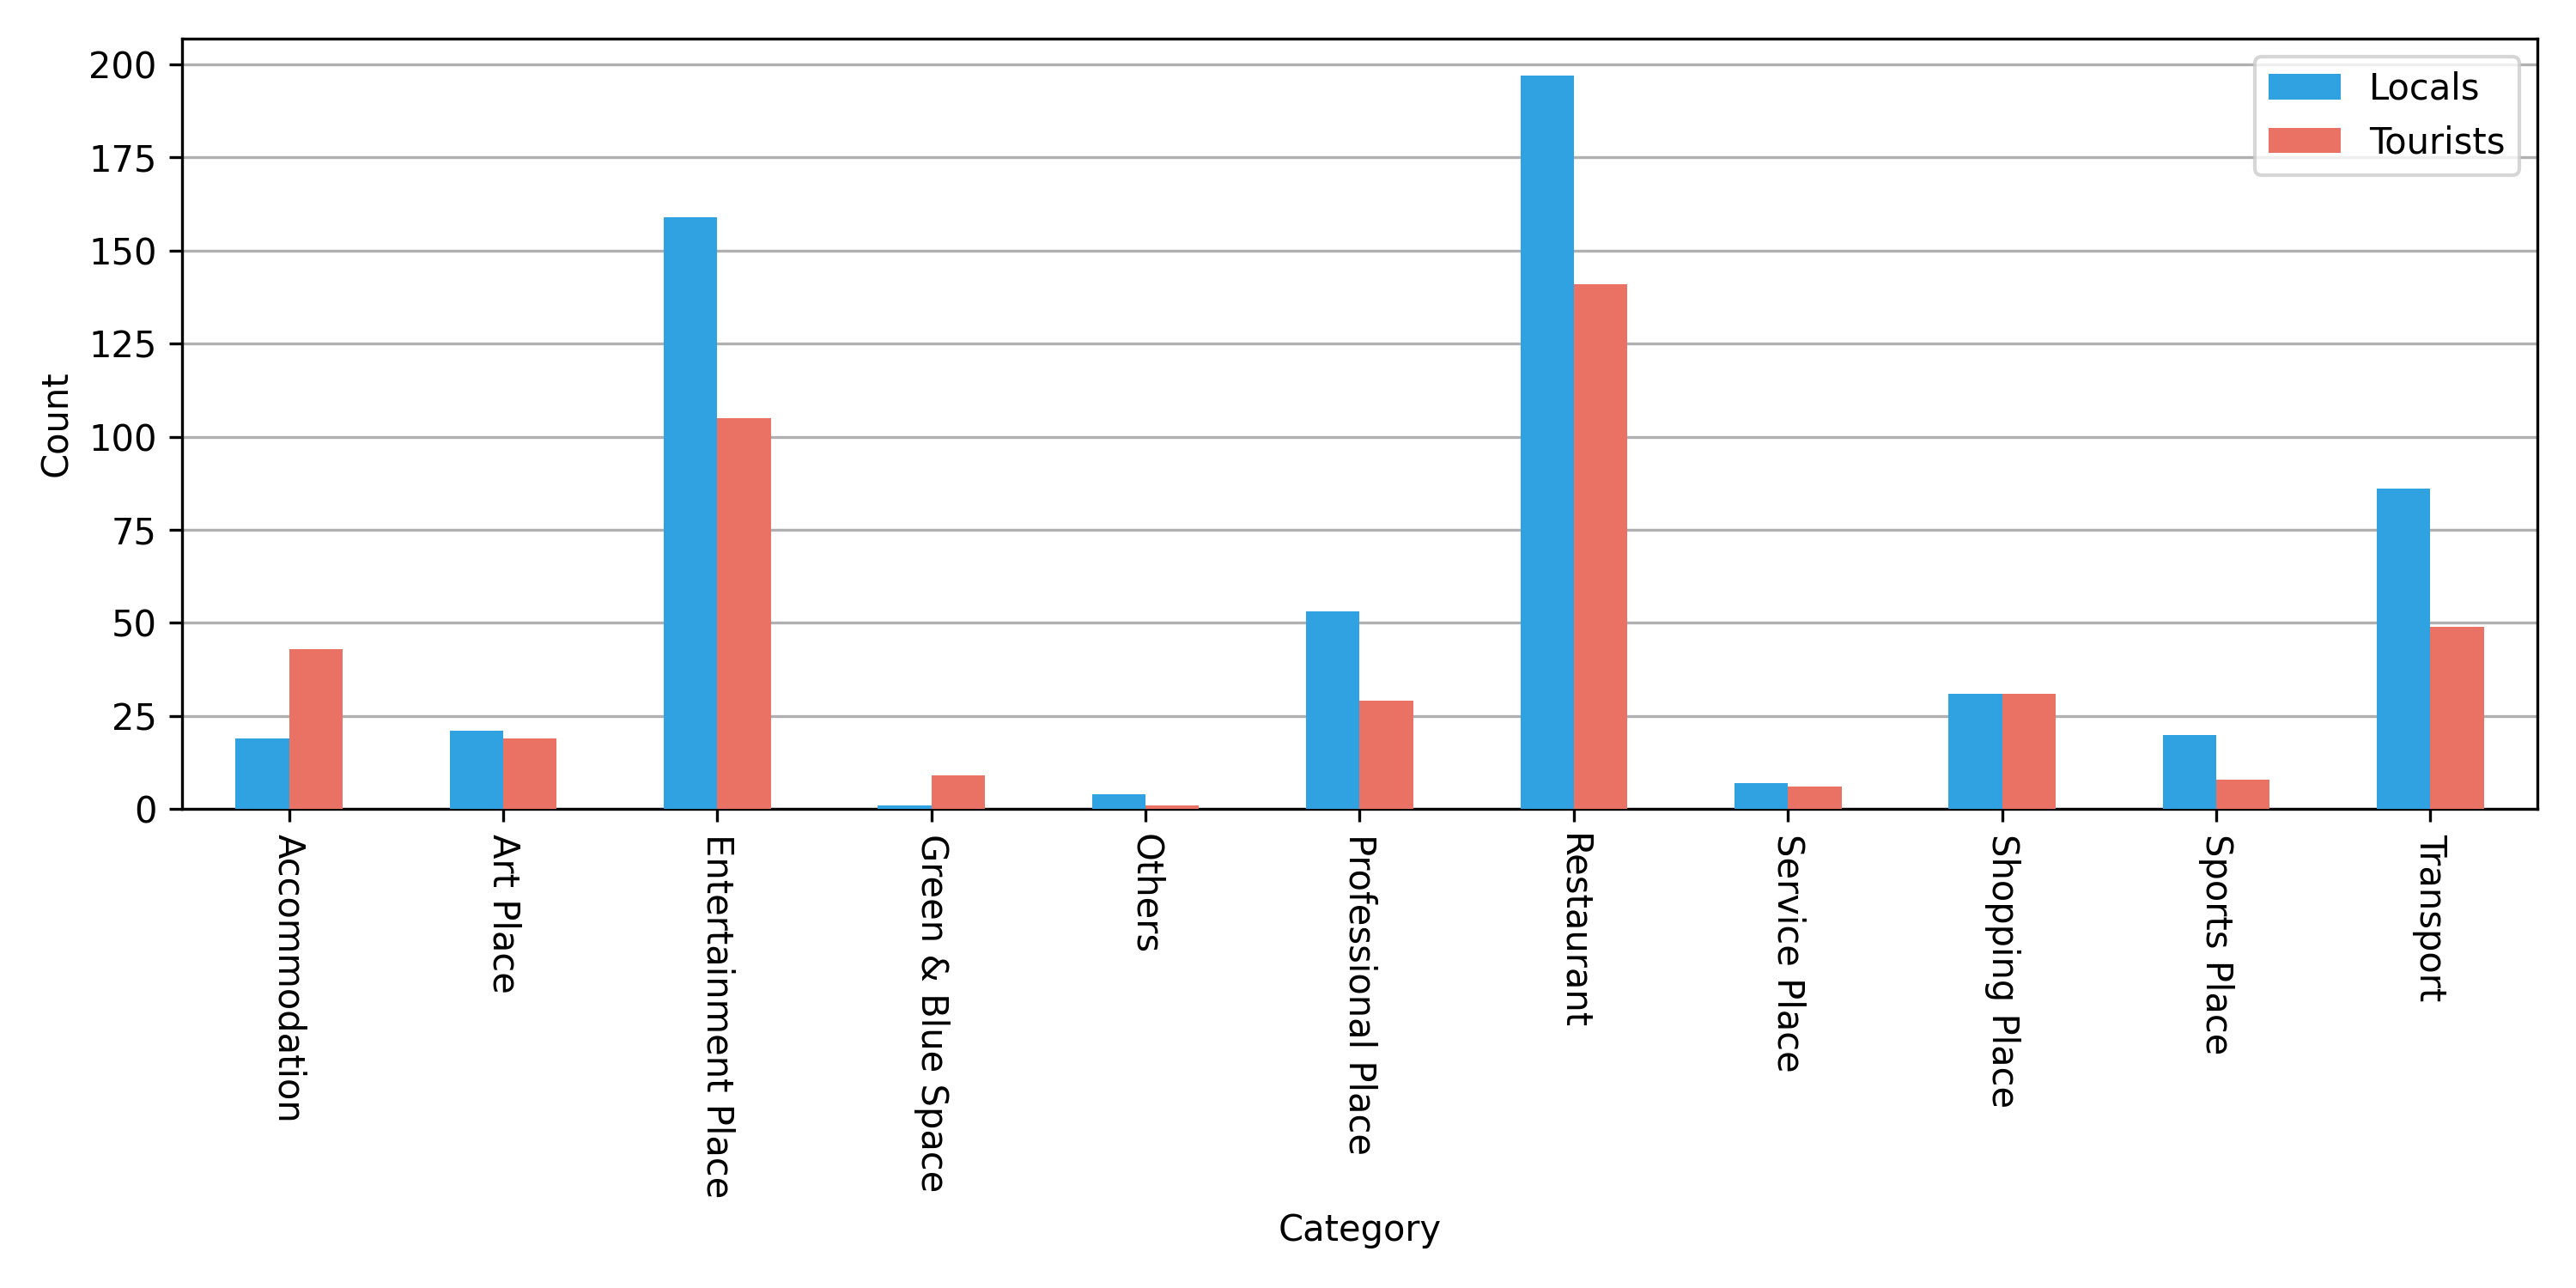
\includegraphics[width=0.9\linewidth]{figures/places_locale_nighttime.png}
\caption{Nighttime.}
\label{fig:places_locale_nighttime}
\end{subfigure}

\caption{Locale dimension of places during the daytime and nighttime.}
\label{fig:places_locale_day}
\end{figure}


\textbf{Sense of Place}

% daytime locals
The distribution of locals' places in the \textit{Sense of Place} dimension of locals during the daytime is shown in Figure~\ref{fig:places_topics_sense_locals_daytime}. Locals' descriptions of places they visit are summarized by eight topics. Over 700 places are characterized by air and rail transportation (e.g., lhr\footnote{The airport London Heathrow.}, airbus, bus, railway), as illustrated in the high frequency of Topic 0 and Topic 4 (Figure~\ref{fig:places_sense_daytime_locals}, Figure~\ref{fig:topics_daytime_locals}). The distribution of topics in Figure~\ref{fig:topics_distribution_daytime_locals} aligns with the topic content. For instance, the city center is characterized by places associated with Topic 1 (e.g., park, museum, spring) and Topic 2 (e.g., june, party, summer). Commonly, this area is recognized as a hub for leisure activities, given its abundance of renowned parks and museums. In addition, since the transport network covers most areas of the city, Topic 4 (e.g., railway, bus, station) has its places distributed across London. And the vicinity of London Stadium (built for the 2012 Olympics) in Stratford, Newham also exhibits a concentration of places associated with Topic 6 (e.g., olympics, paralympics).


\begin{figure}[!h]
    \centering
    \begin{subfigure}{0.45\textwidth}
        \centering
        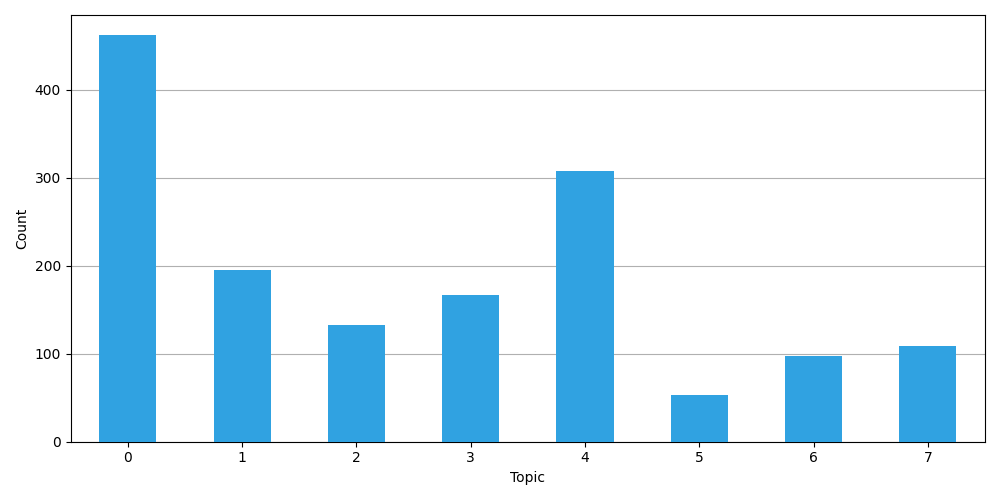
\includegraphics[width=\linewidth]{figures/places_sense_daytime_locals.png} 
        \caption{Frequency of topics.}
        \label{fig:places_sense_daytime_locals}
    \end{subfigure}
    \hfill
    \begin{subfigure}{0.5\textwidth}
        \centering
        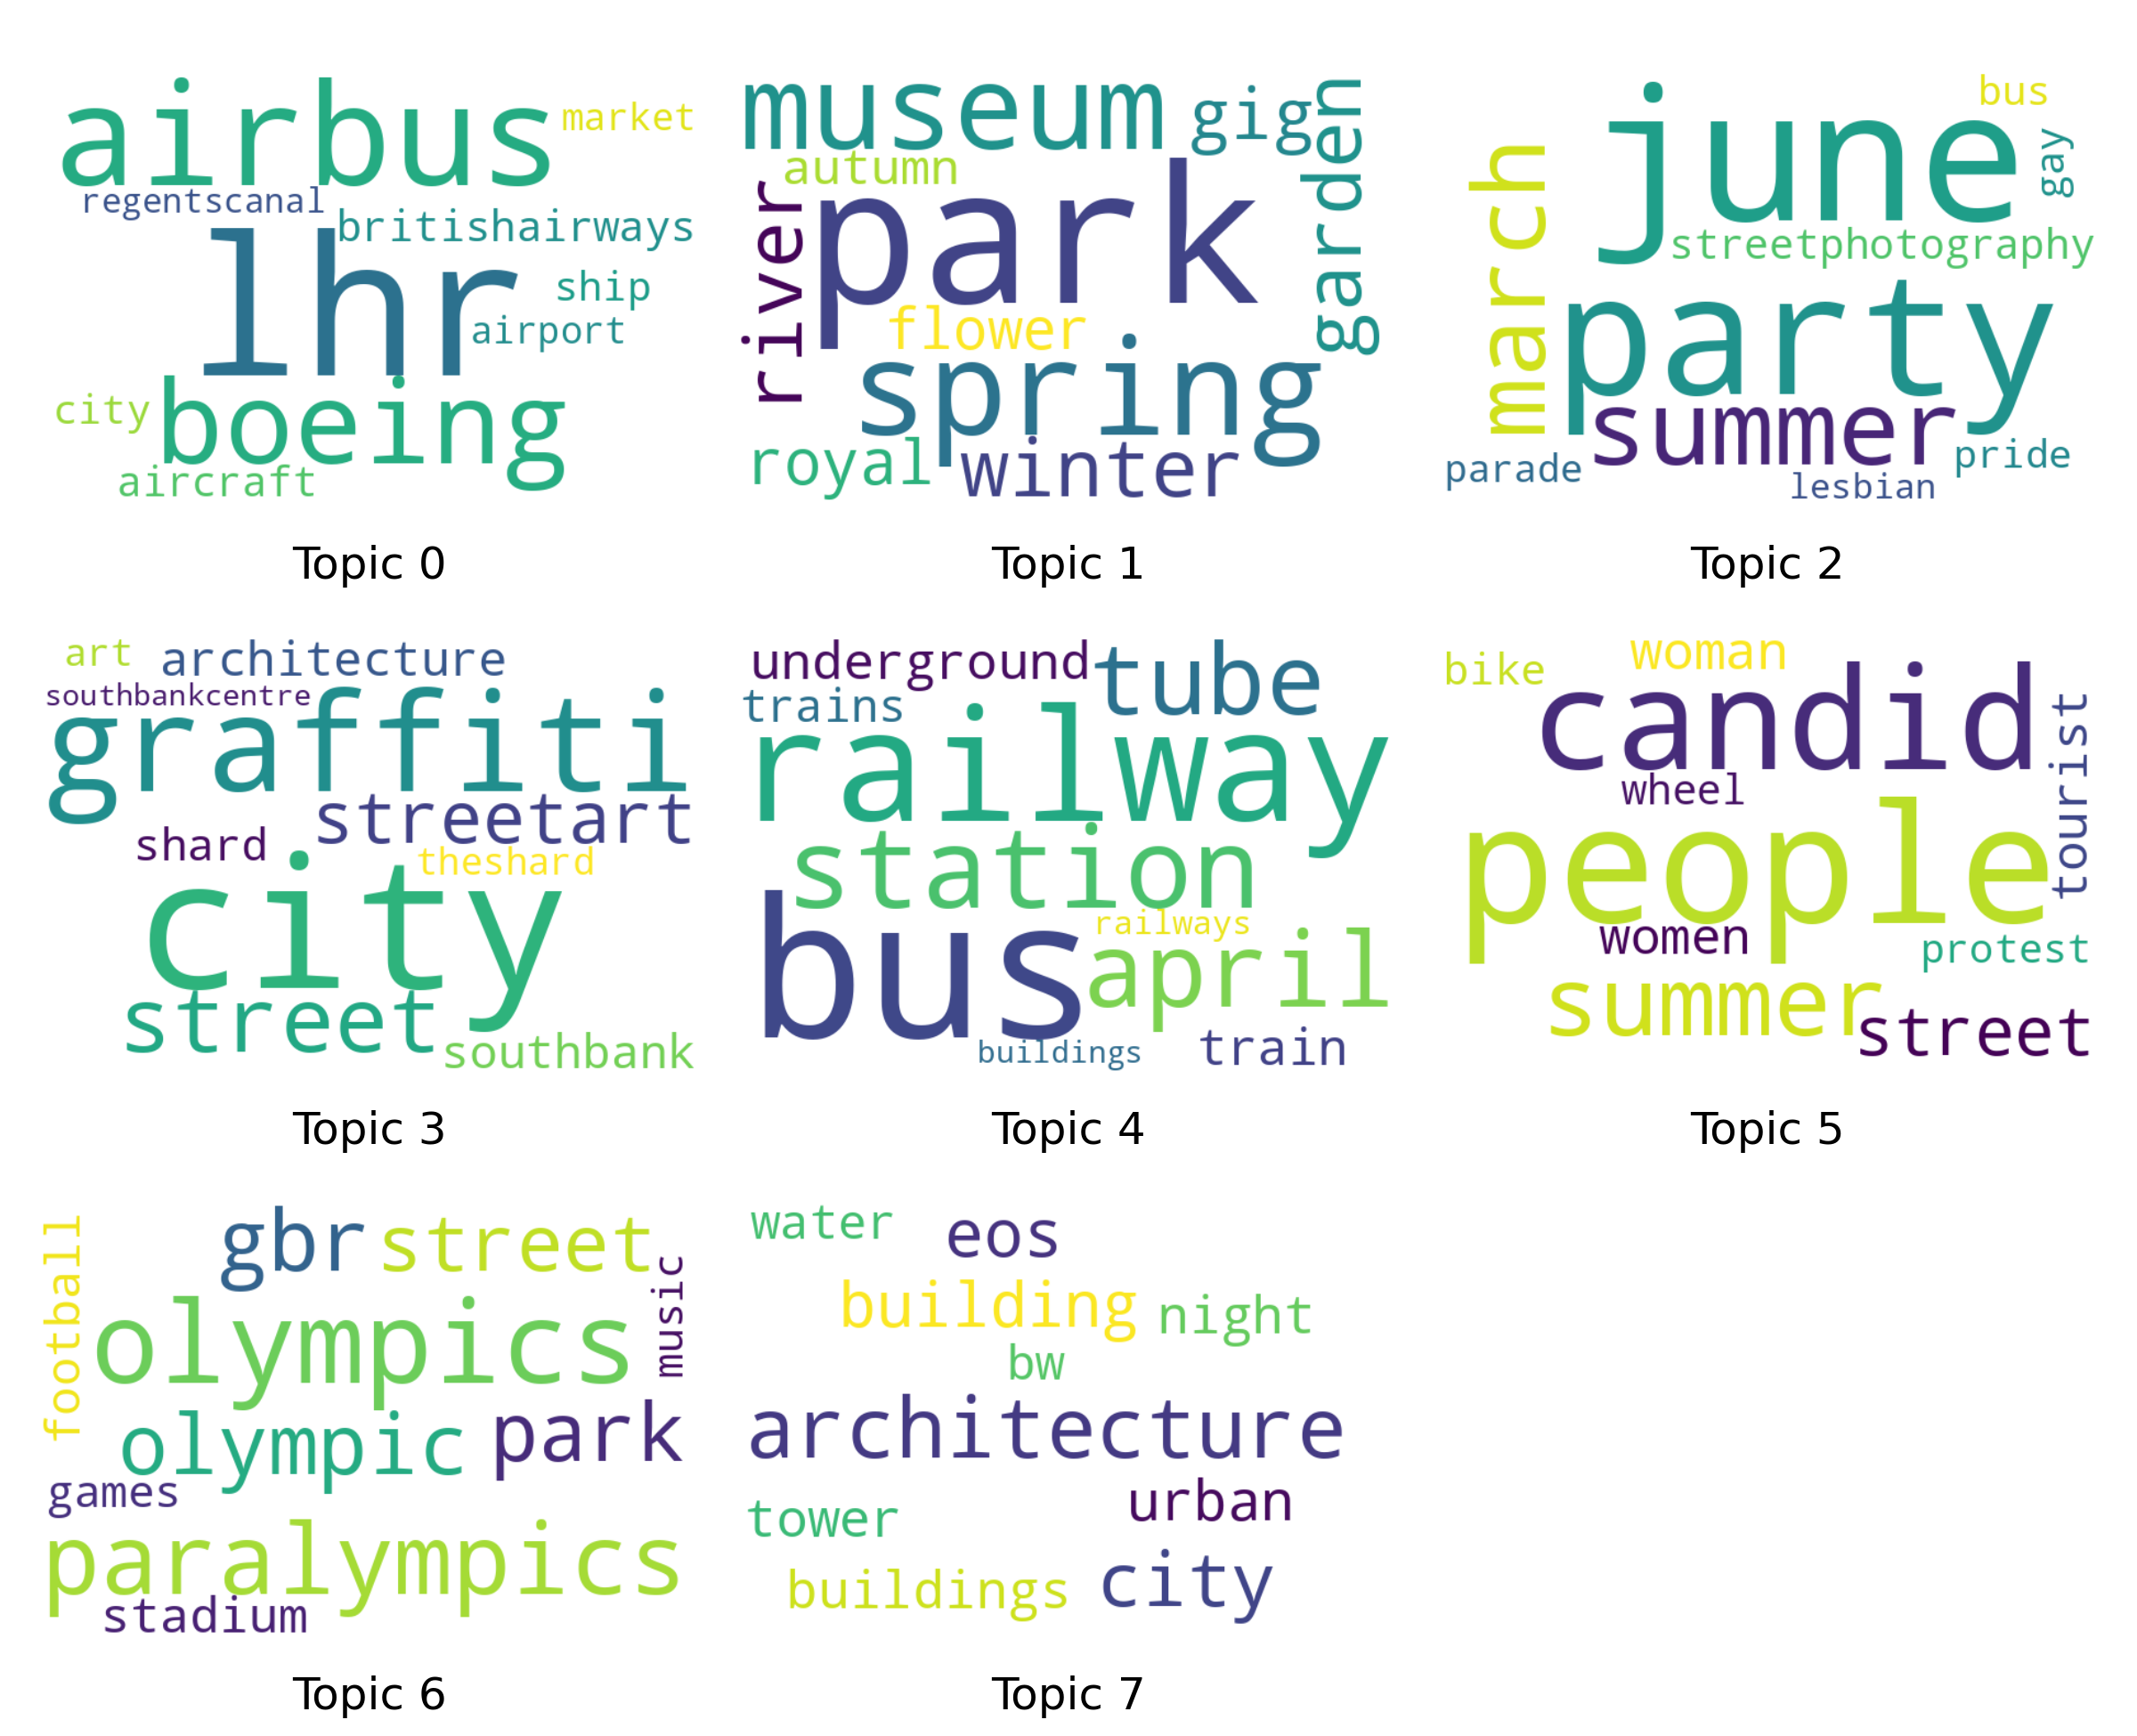
\includegraphics[width=\linewidth]{figures/topics_daytime_locals.png} 
        \caption{Word clouds for topics.}
        \label{fig:topics_daytime_locals}
    \end{subfigure}
    
    \begin{subfigure}{0.9\textwidth}
        \centering
        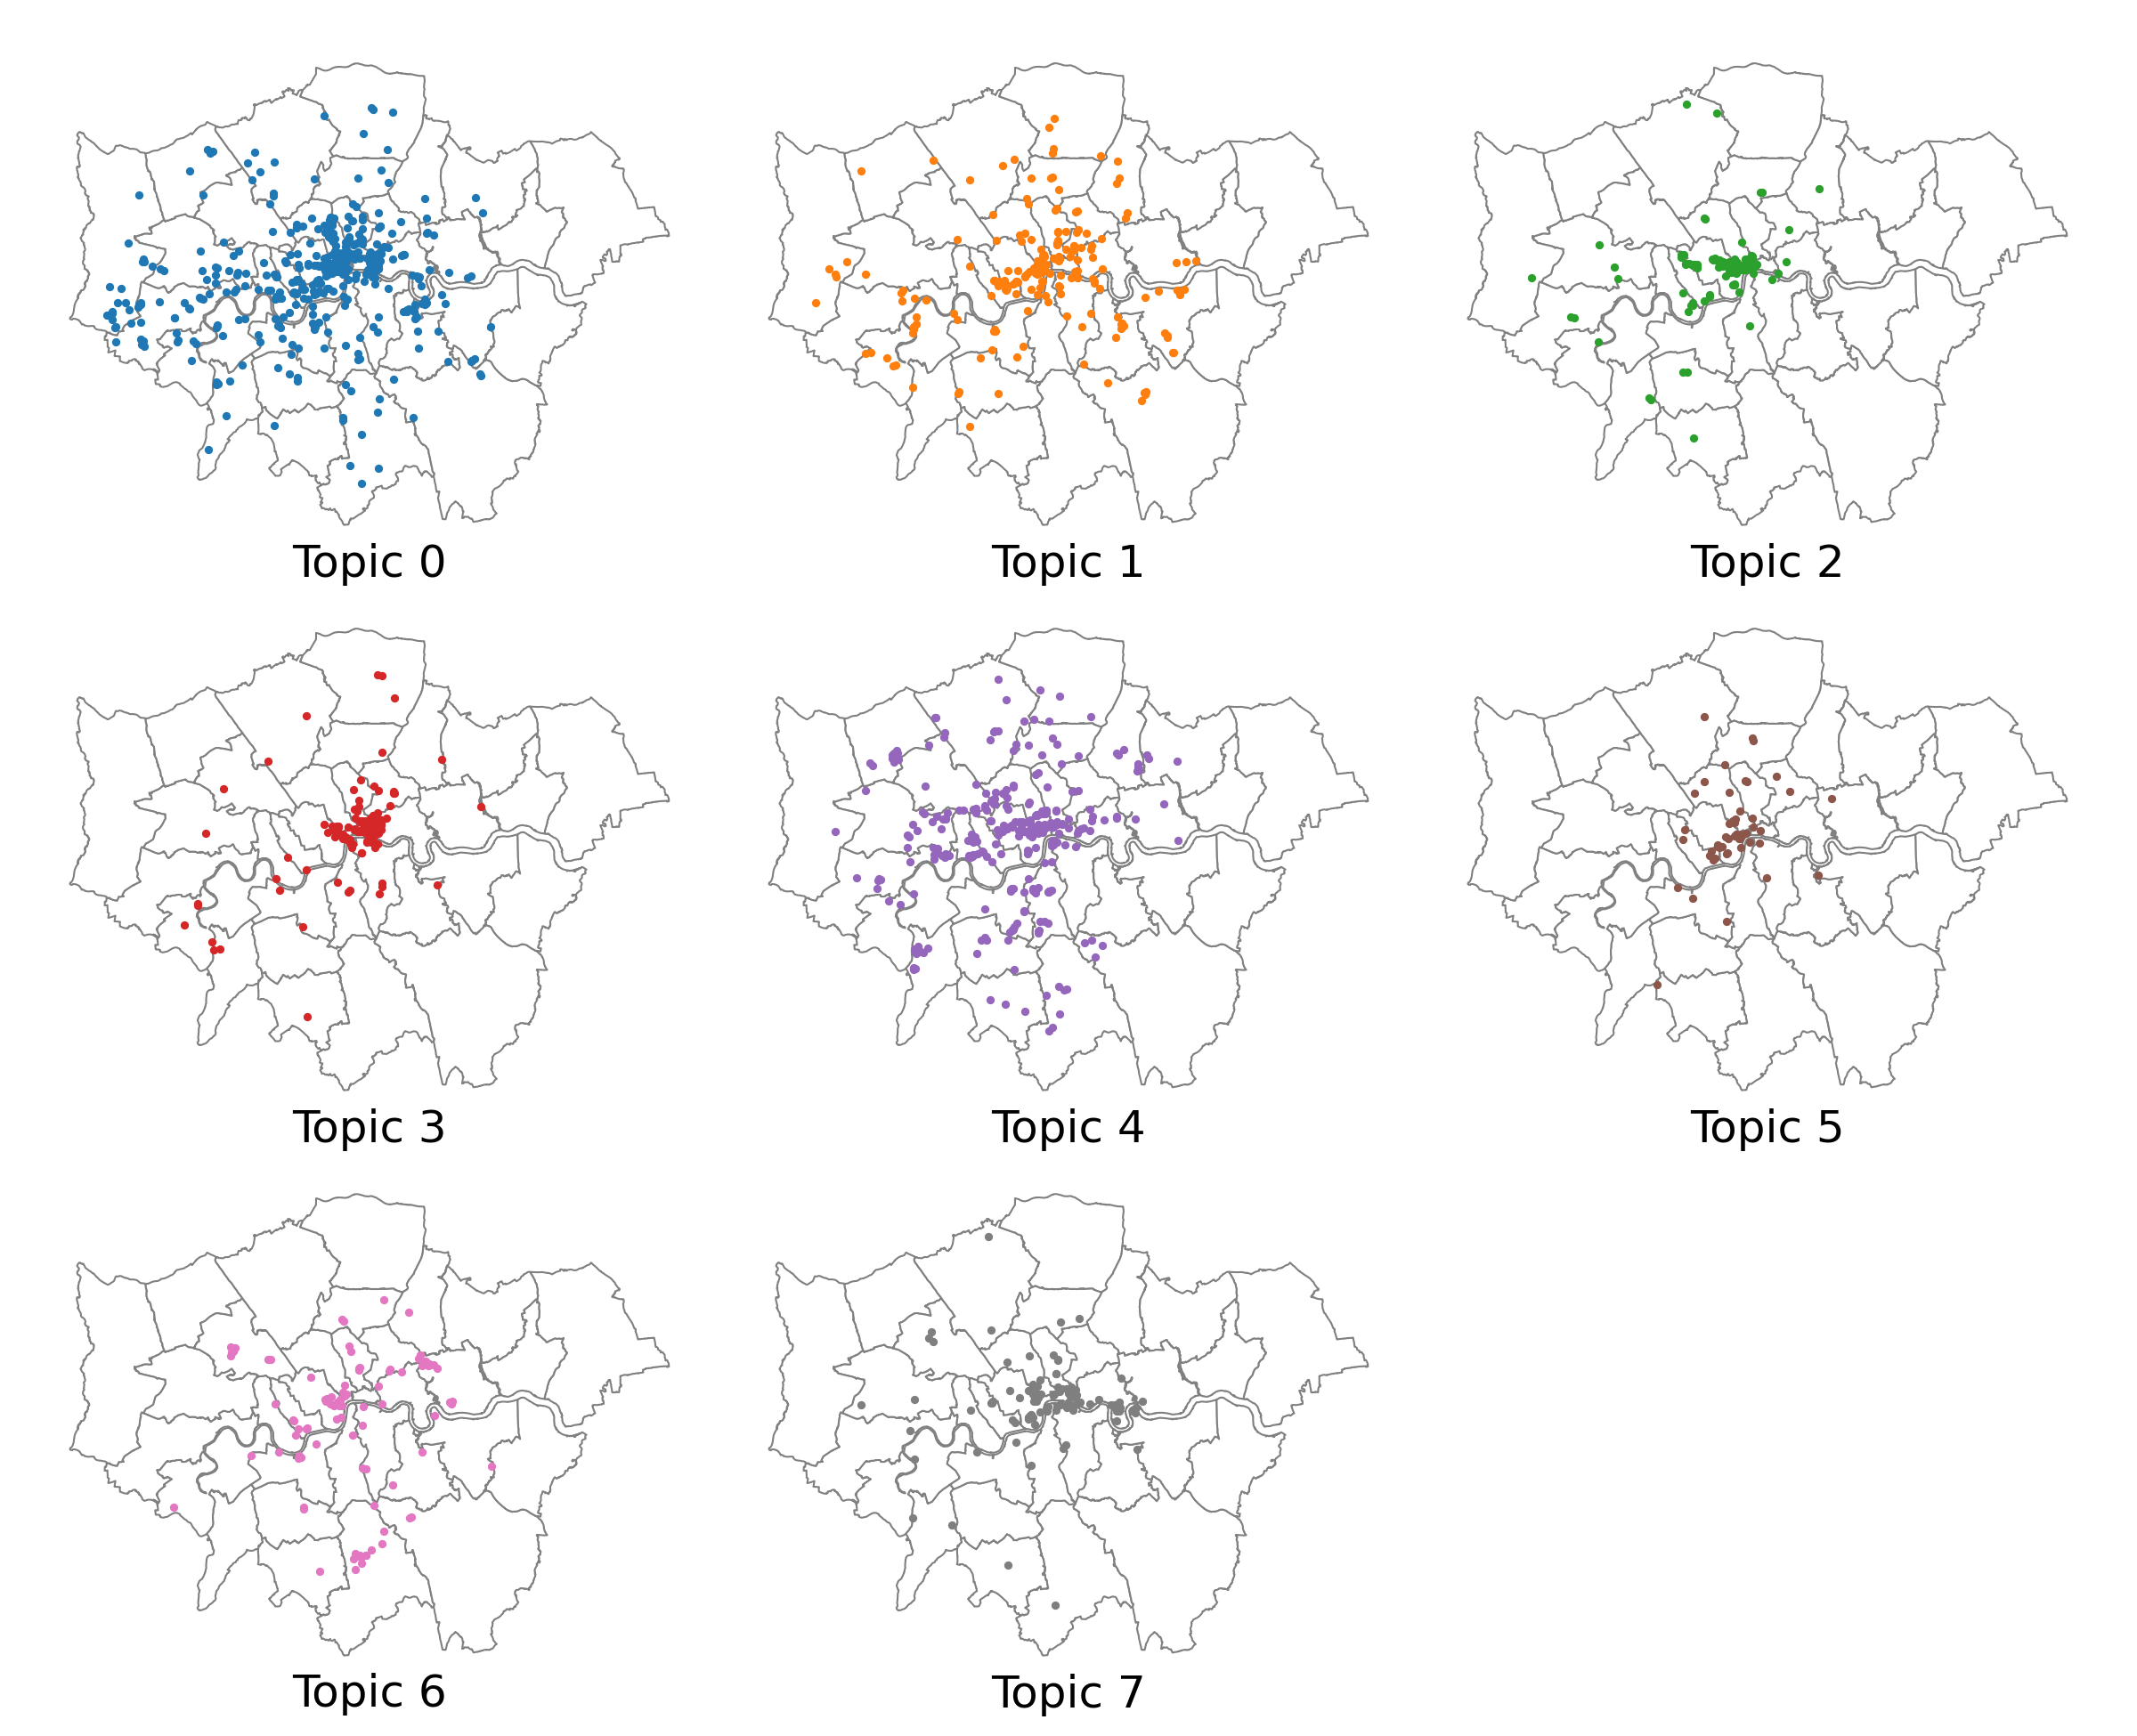
\includegraphics[width=\linewidth]{figures/topics_distribution_daytime_locals.png} 
        \caption{Distribution of topics.}
        \label{fig:topics_distribution_daytime_locals}
    \end{subfigure}

    \caption{Sense of place dimension of locals' places during the daytime.}
    \label{fig:places_topics_sense_locals_daytime}
\end{figure}

% daytime tourists
In terms of tourists' daytime places in the \textit{Sense of Place} dimension, six topics are generated to describe these places (Figure~\ref{fig:places_topics_sense_tourists_daytime}). Compared to locals, tourists during the daytime demonstrate a preference for urban-related places (Topic 4) and the Olympics (Topic 0), with the number of associated places exceeding 350 and 250 respectively. Places related to air transport are less popular among tourists, as shown in the low frequency of Topic 1 (e.g., lhr, aircraft, airbus) (Figure~\ref{fig:places_sense_daytime_tourists}, Figure~\ref{fig:topics_daytime_tourists}). Figure~\ref{fig:topics_distribution_daytime_tourists} displays the spatial distribution of topics. The inner part of London is representative of urban life with numerous art venues, thus this area exhibits a concentration of Topic 4 (e.g., street, bus, city) and Topic 5 (e.g., museum, art, architecture). Places in Topic 1 are predominantly near Heathrow Airport, which is highly related to the topic content. Topic 2 describes places along the bustling part of the River Thames with tags like tower, city, bridge, and river. Additionally, topics related to the Olympics also show distinct distribution patterns. Topic 0 (e.g., olympics, paralympics) covers areas not only around London Stadium but also the city center. Moreover, similar to the route of the London 2012 Olympic Marathon, places in Topic 3 (e.g., marathon, city, urban) are mainly distributed along the River Thames.

\begin{figure}[!h]
    \centering
    \begin{subfigure}{0.45\textwidth}
        \centering
        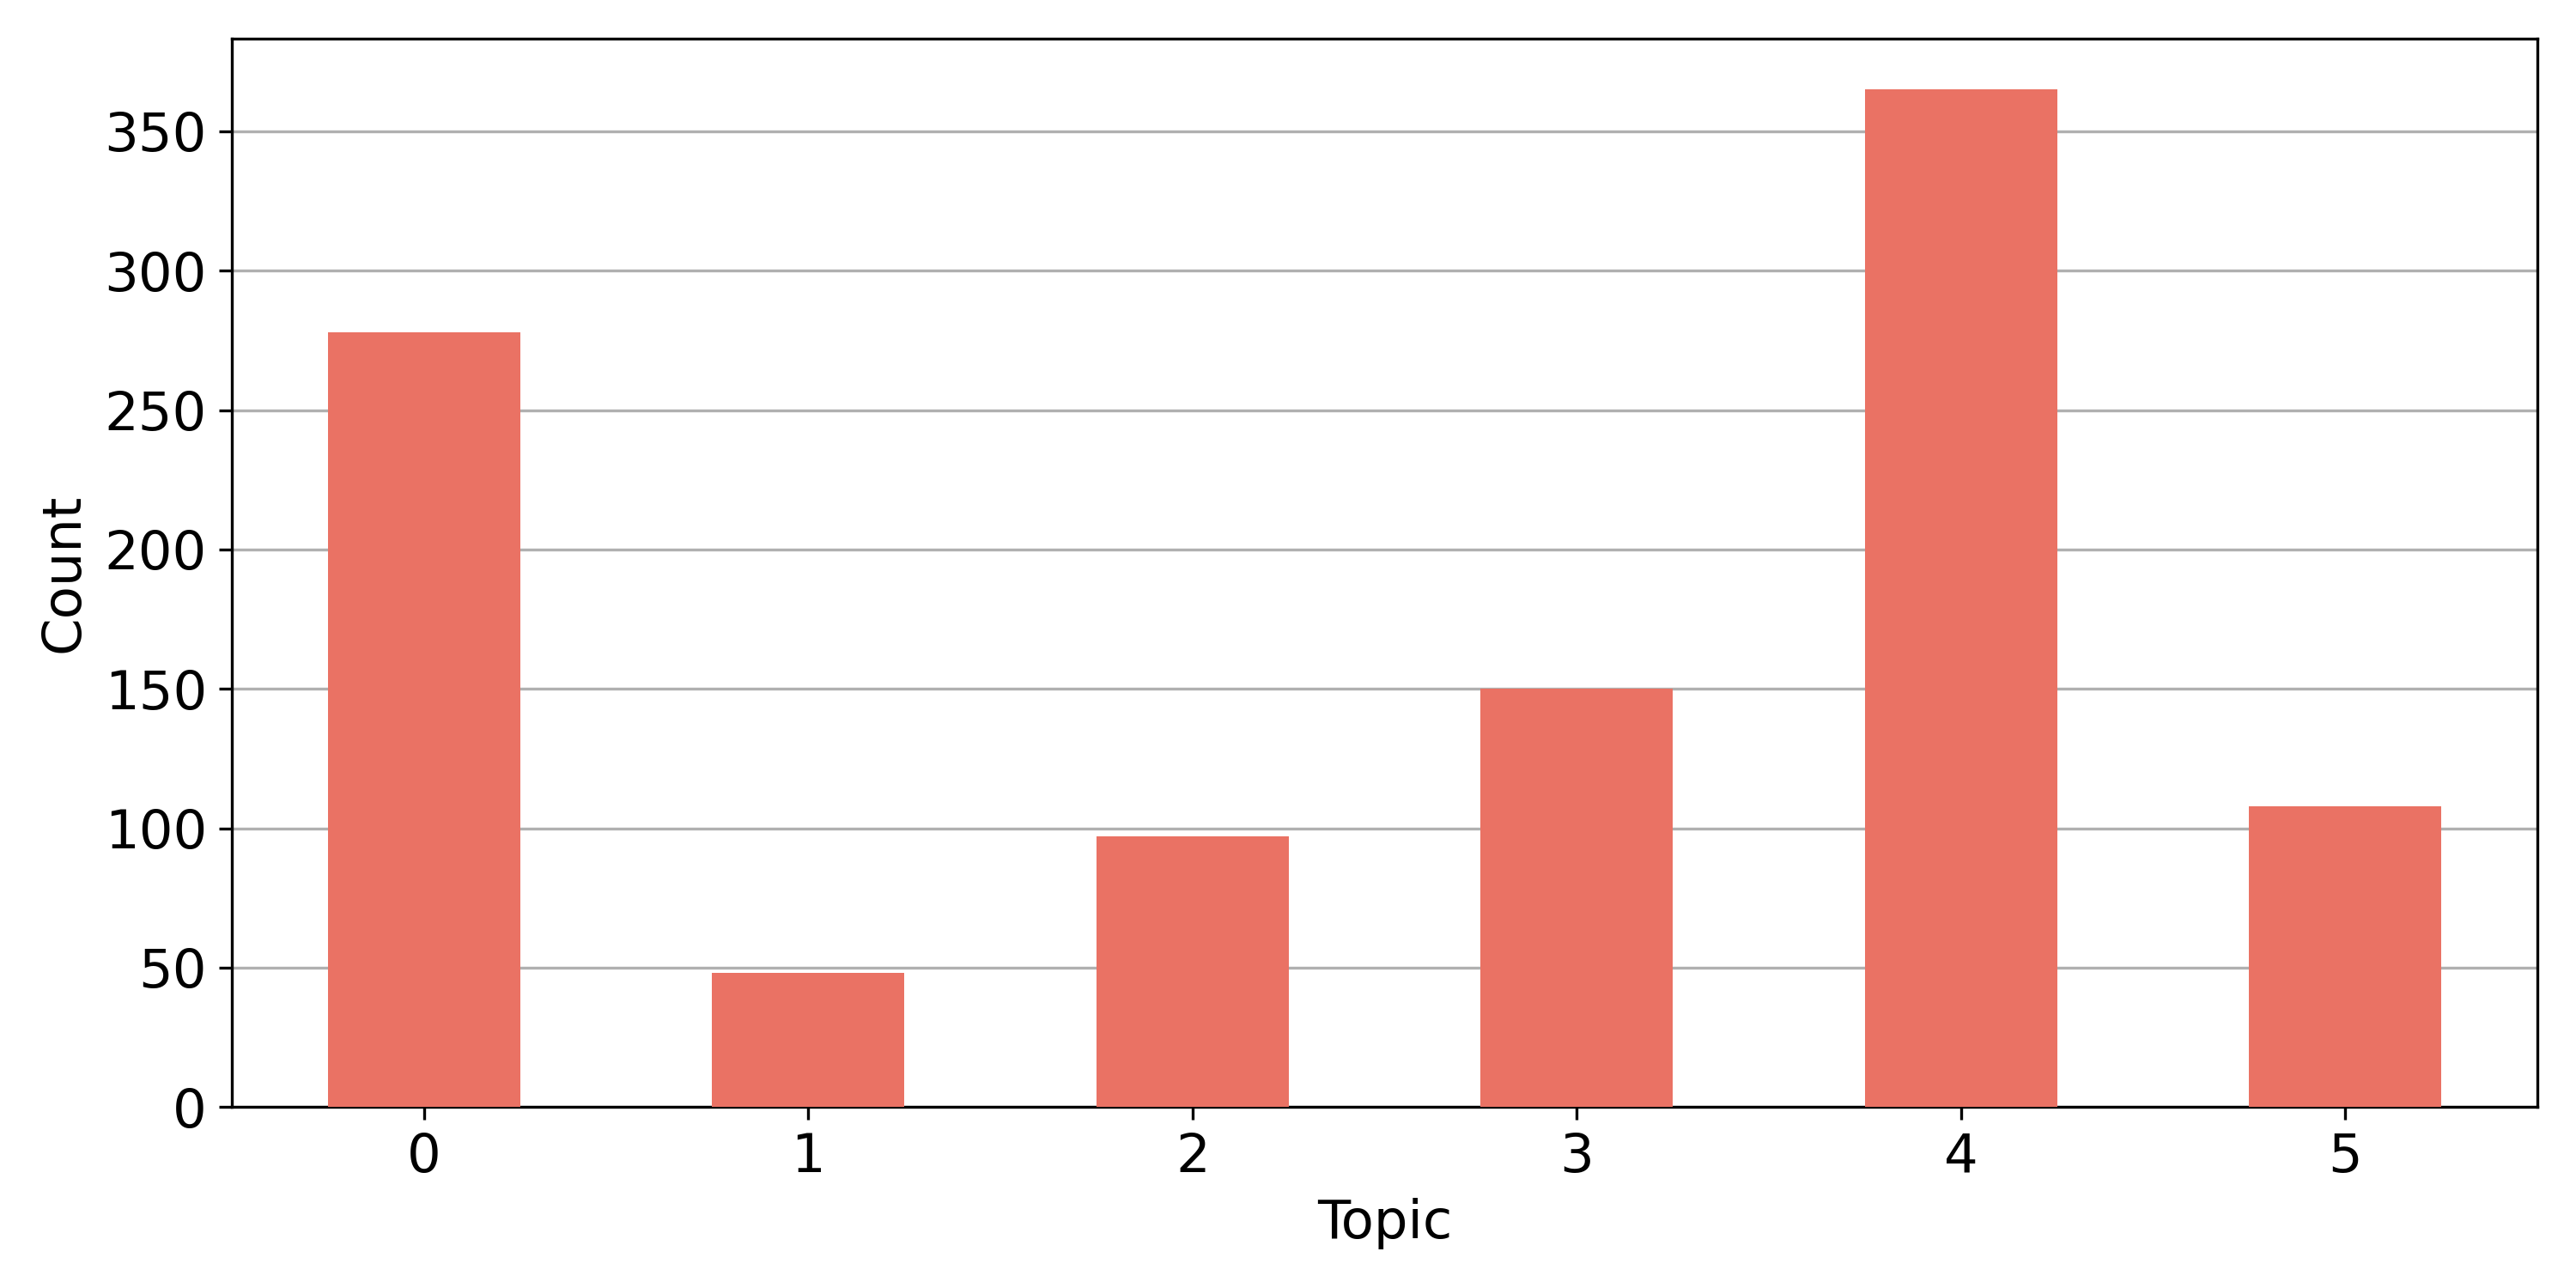
\includegraphics[width=\linewidth]{figures/places_sense_daytime_tourists.png} 
        \caption{Frequency of topics.}
        \label{fig:places_sense_daytime_tourists}
    \end{subfigure}
    \hfill
    \begin{subfigure}{0.5\textwidth}
        \centering
        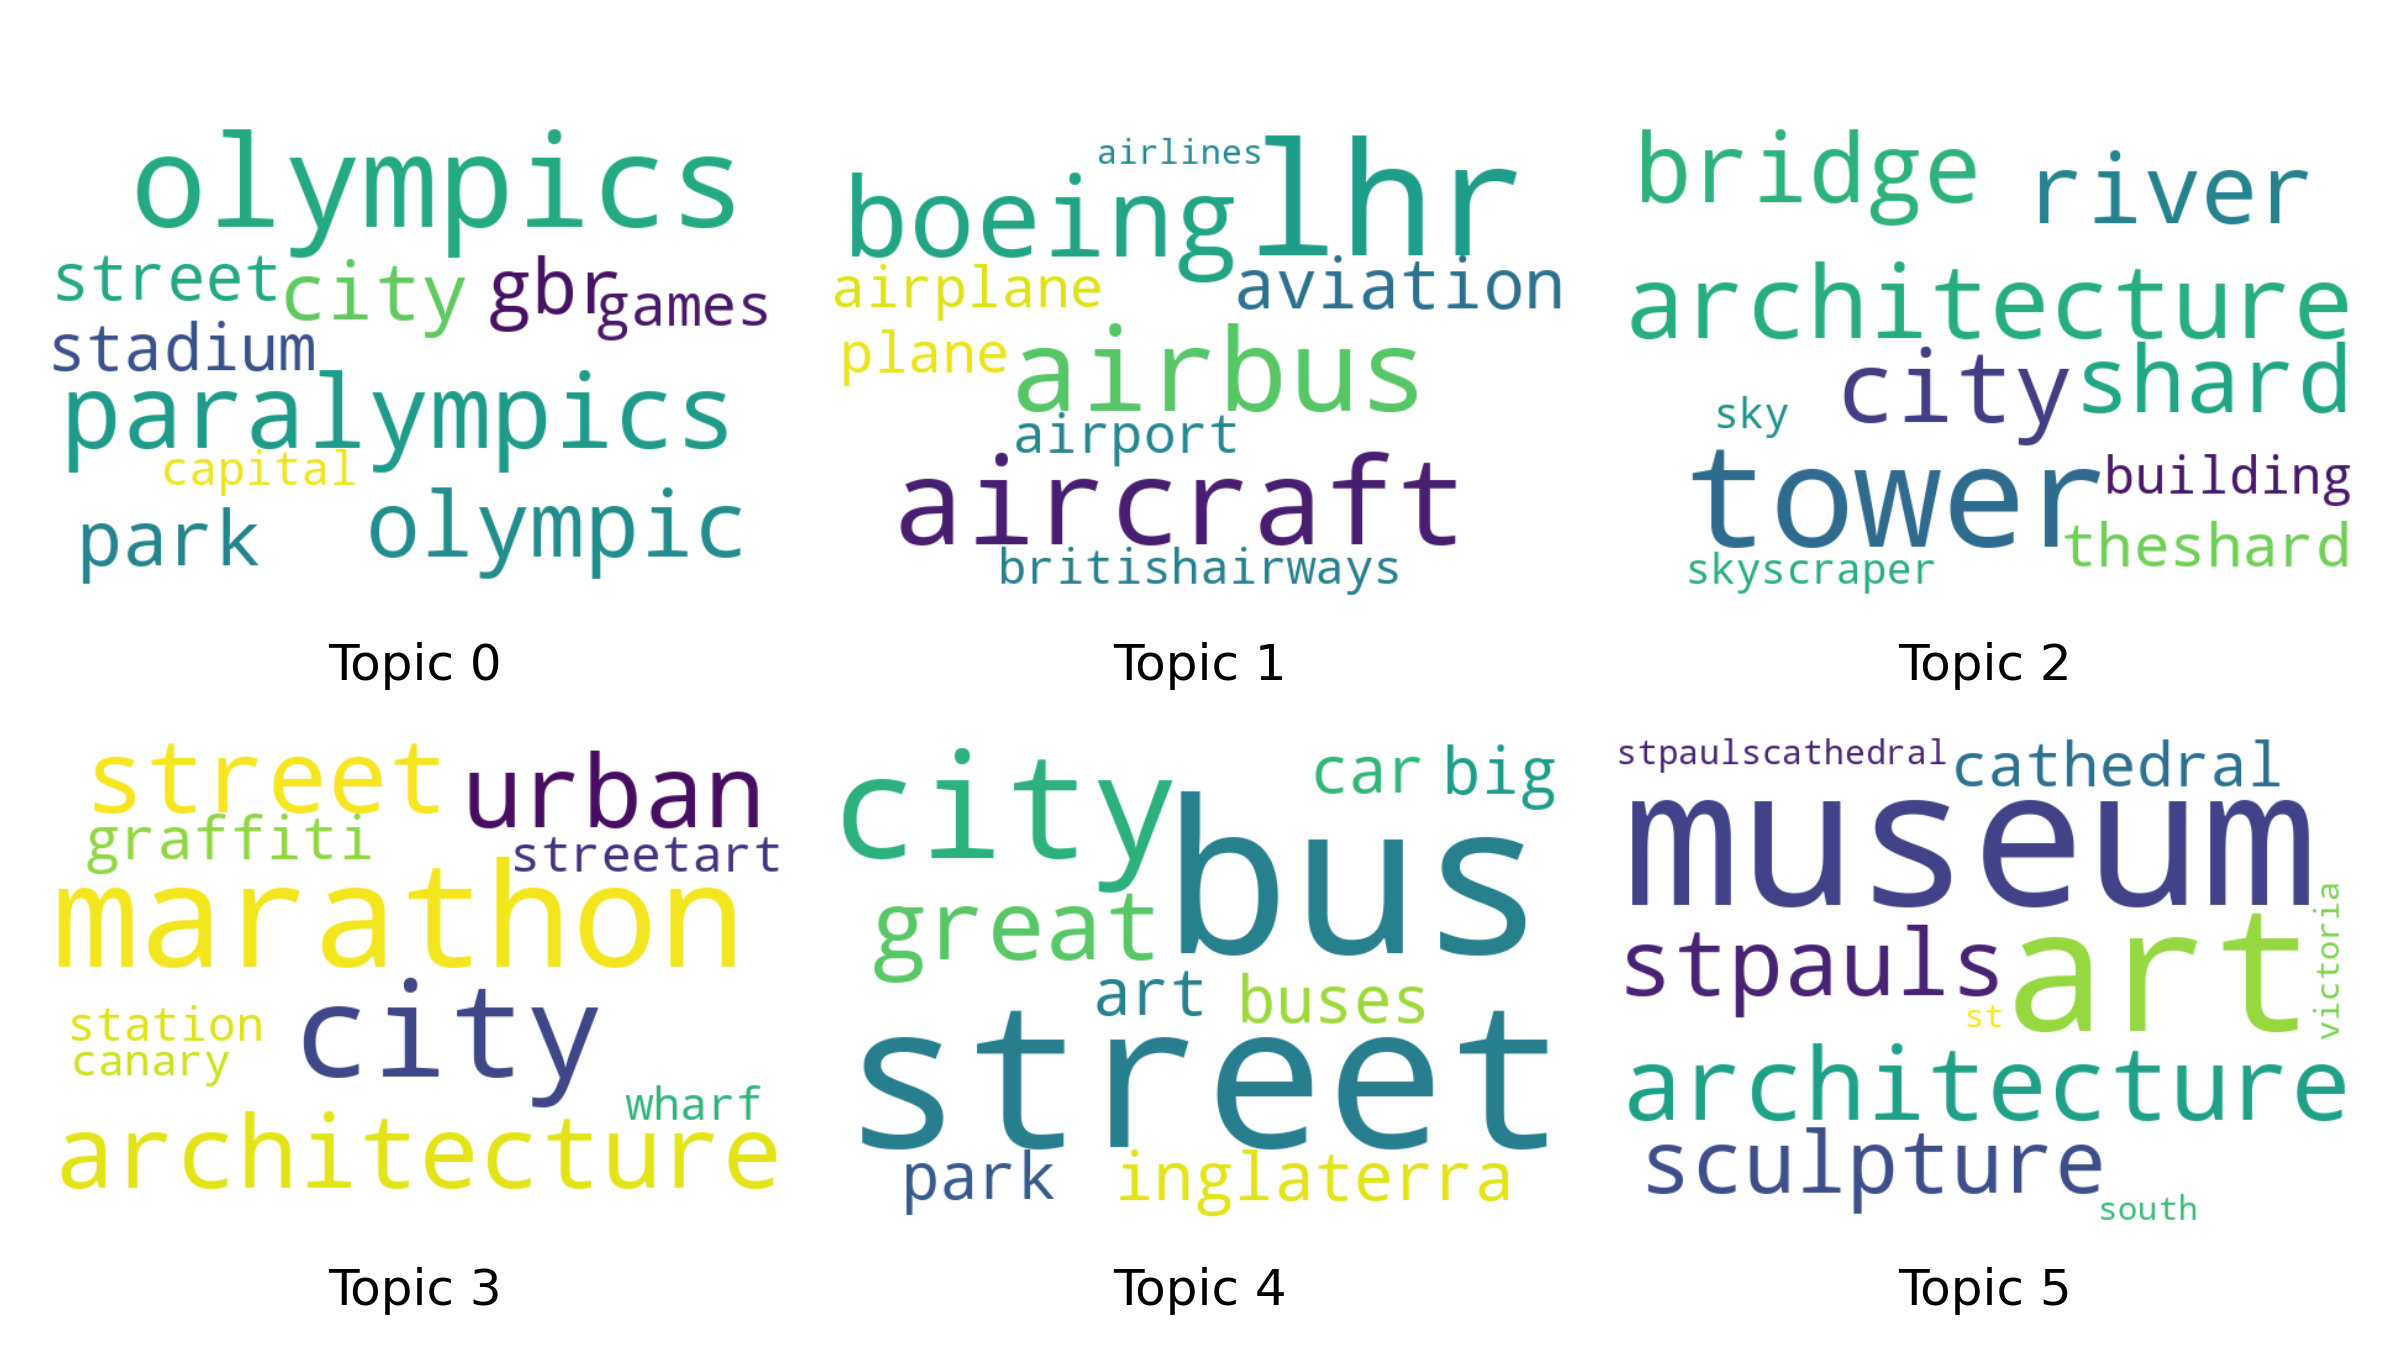
\includegraphics[width=\linewidth]{figures/topics_daytime_tourists.png} 
        \caption{Word clouds for topics.}
        \label{fig:topics_daytime_tourists}
    \end{subfigure}
    
    \begin{subfigure}{0.9\textwidth}
        \centering
        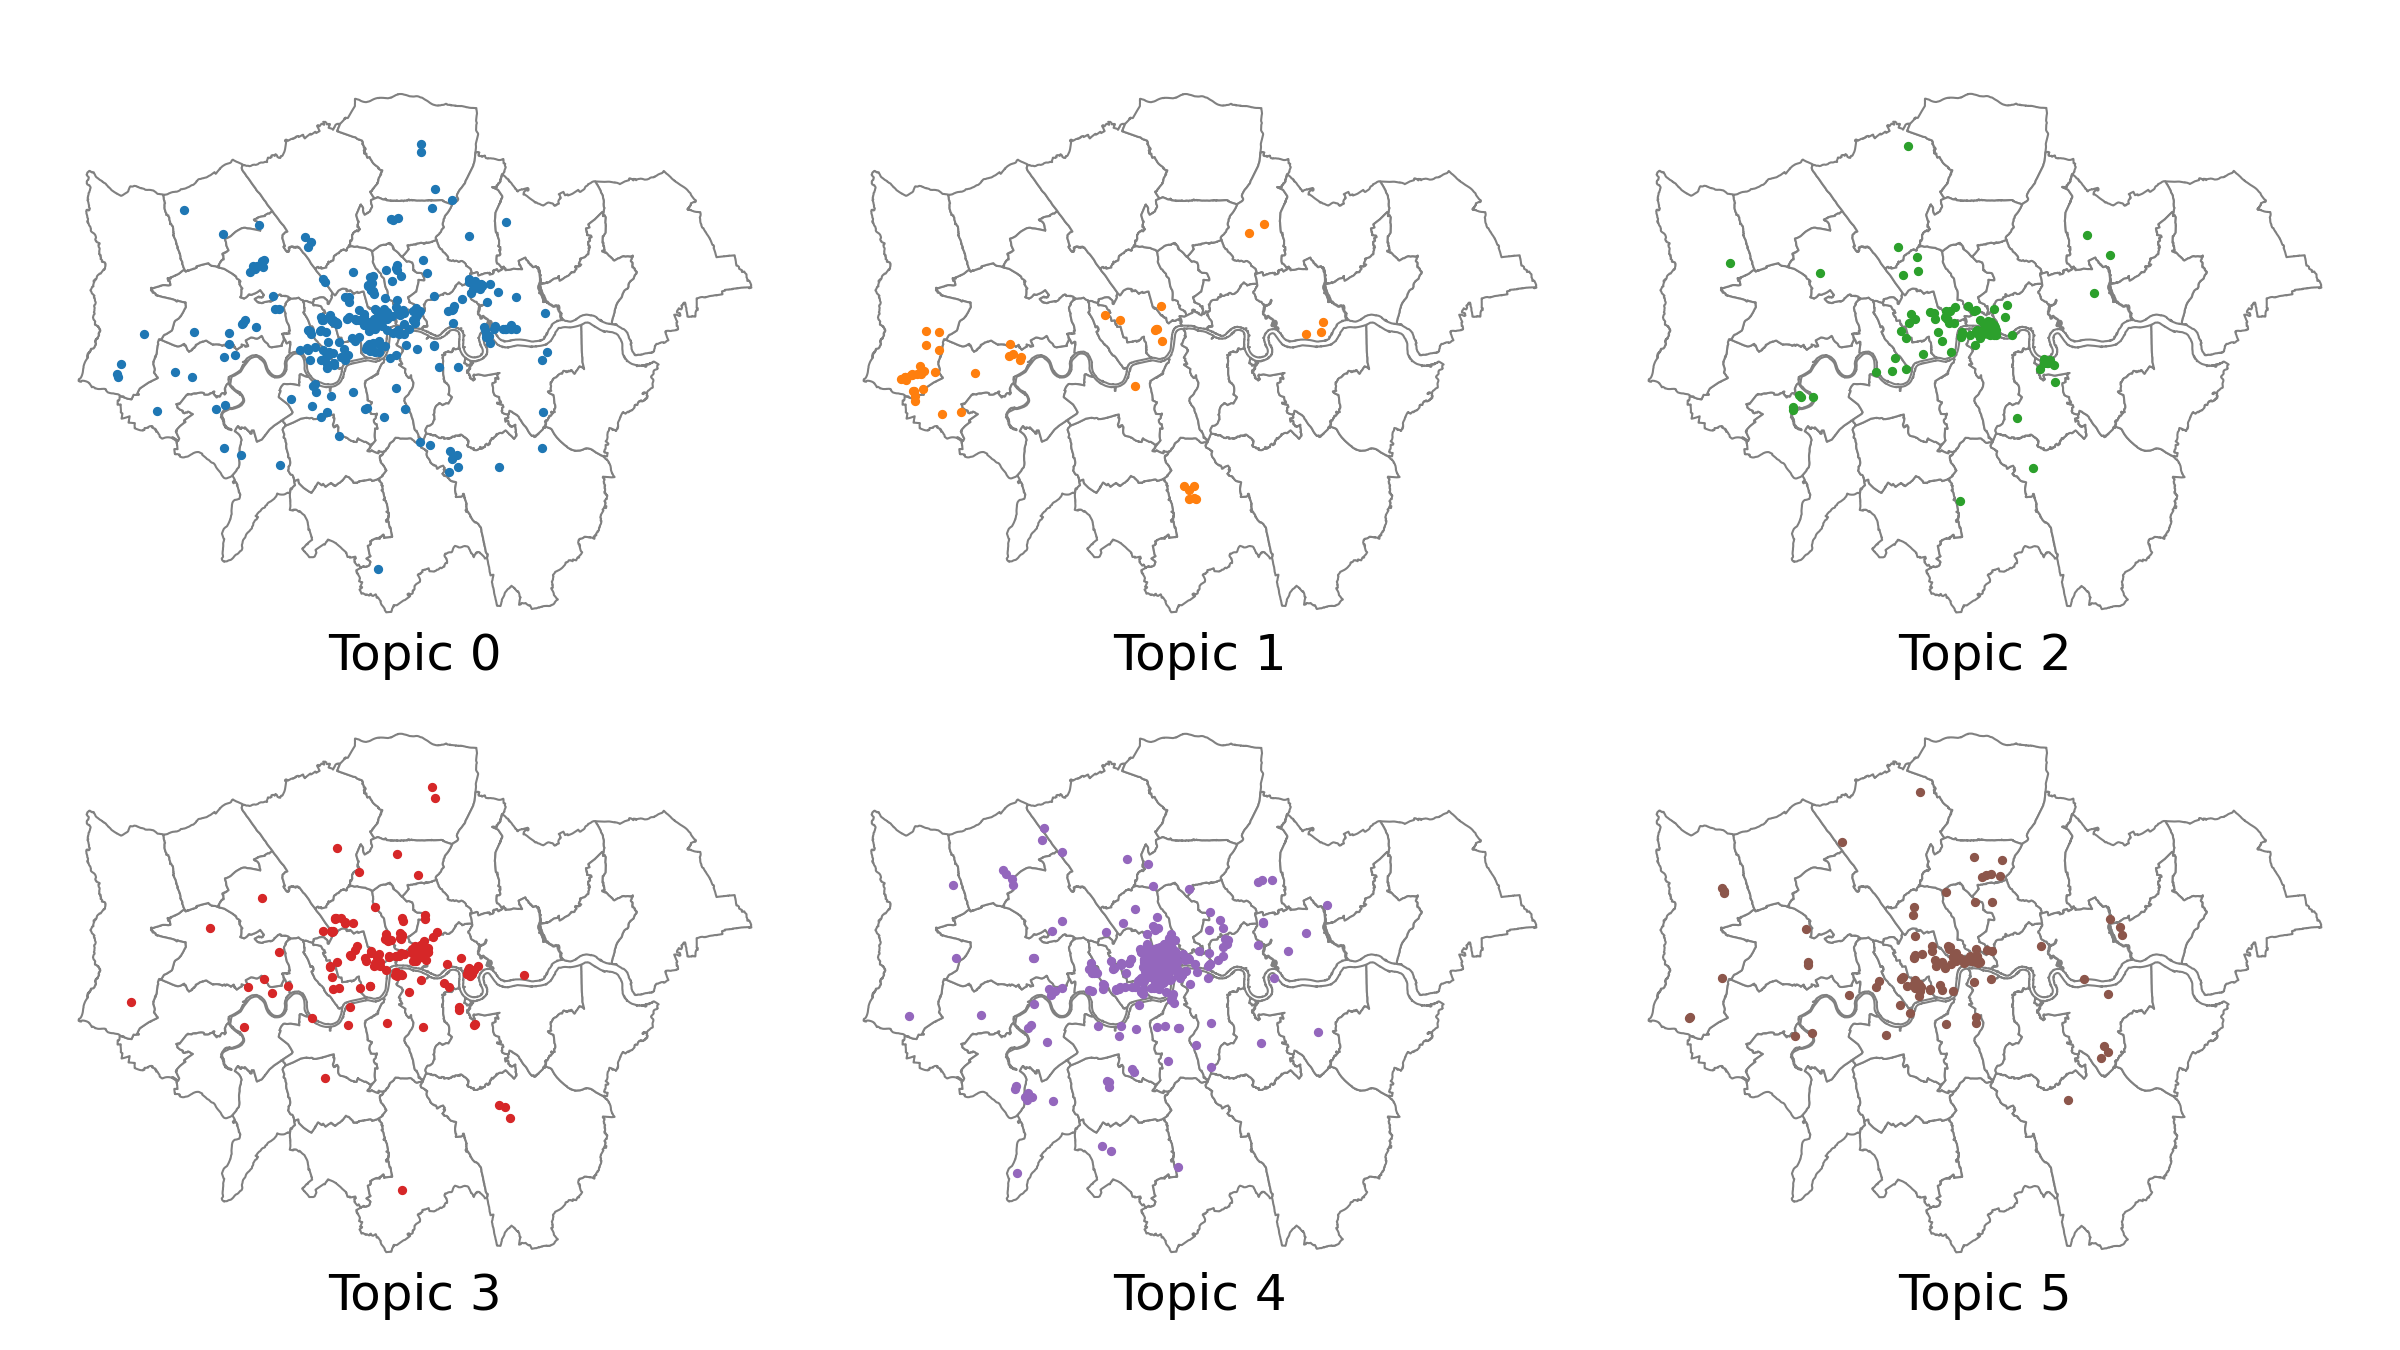
\includegraphics[width=\linewidth]{figures/topics_distribution_daytime_tourists.png} 
        \caption{Distribution of topics.}
        \label{fig:topics_distribution_daytime_tourists}
    \end{subfigure}

    \caption{Sense of place dimension of tourists' places during the daytime.}
    \label{fig:places_topics_sense_tourists_daytime}
\end{figure}

% nighttime locals
As night falls, locals' descriptions of London are summarized by six topics (Figure~\ref{fig:places_topics_sense_locals_nighttime}). Topics during this period start to include words related to nighttime venues and events. Locals discuss live, music, gig, and concert, indicating a shift towards more leisurely activities. In terms of the frequency of topics, Topic 0 (e.g., paralympics, crowd, cycling, performance) emerges as the most popular topic, with approximately 300 associated places. The remaining five topics are less frequently mentioned, each comprising fewer than 100 places (Figure~\ref{fig:places_sense_nighttime_locals}, Figure~\ref{fig:topics_nighttime_locals}). Figure~\ref{fig:topics_distribution_nighttime_locals} displays the distribution of topics. Topic 1 (e.g., gig, live, street), Topic 2 (e.g., Charlie, bar, wrights, party), Topic 4 (e.g., bbc, music, gig), and Topic 5 (e.g., people, night, candid, party) are more related to nighttime activities. Topic 1 predominantly features places in Westminster, known for its vibrant gig and live music venues in the evening. Topic 2 concentrates its places in the vicinity of Shoreditch, where a multitude of bars and clubs are located. Topic 4 and Topic 5 display a more dispersed distribution of places, reaching the outskirts boroughs.

\begin{figure}[!h]
    \centering
    \begin{subfigure}{0.45\textwidth}
        \centering
        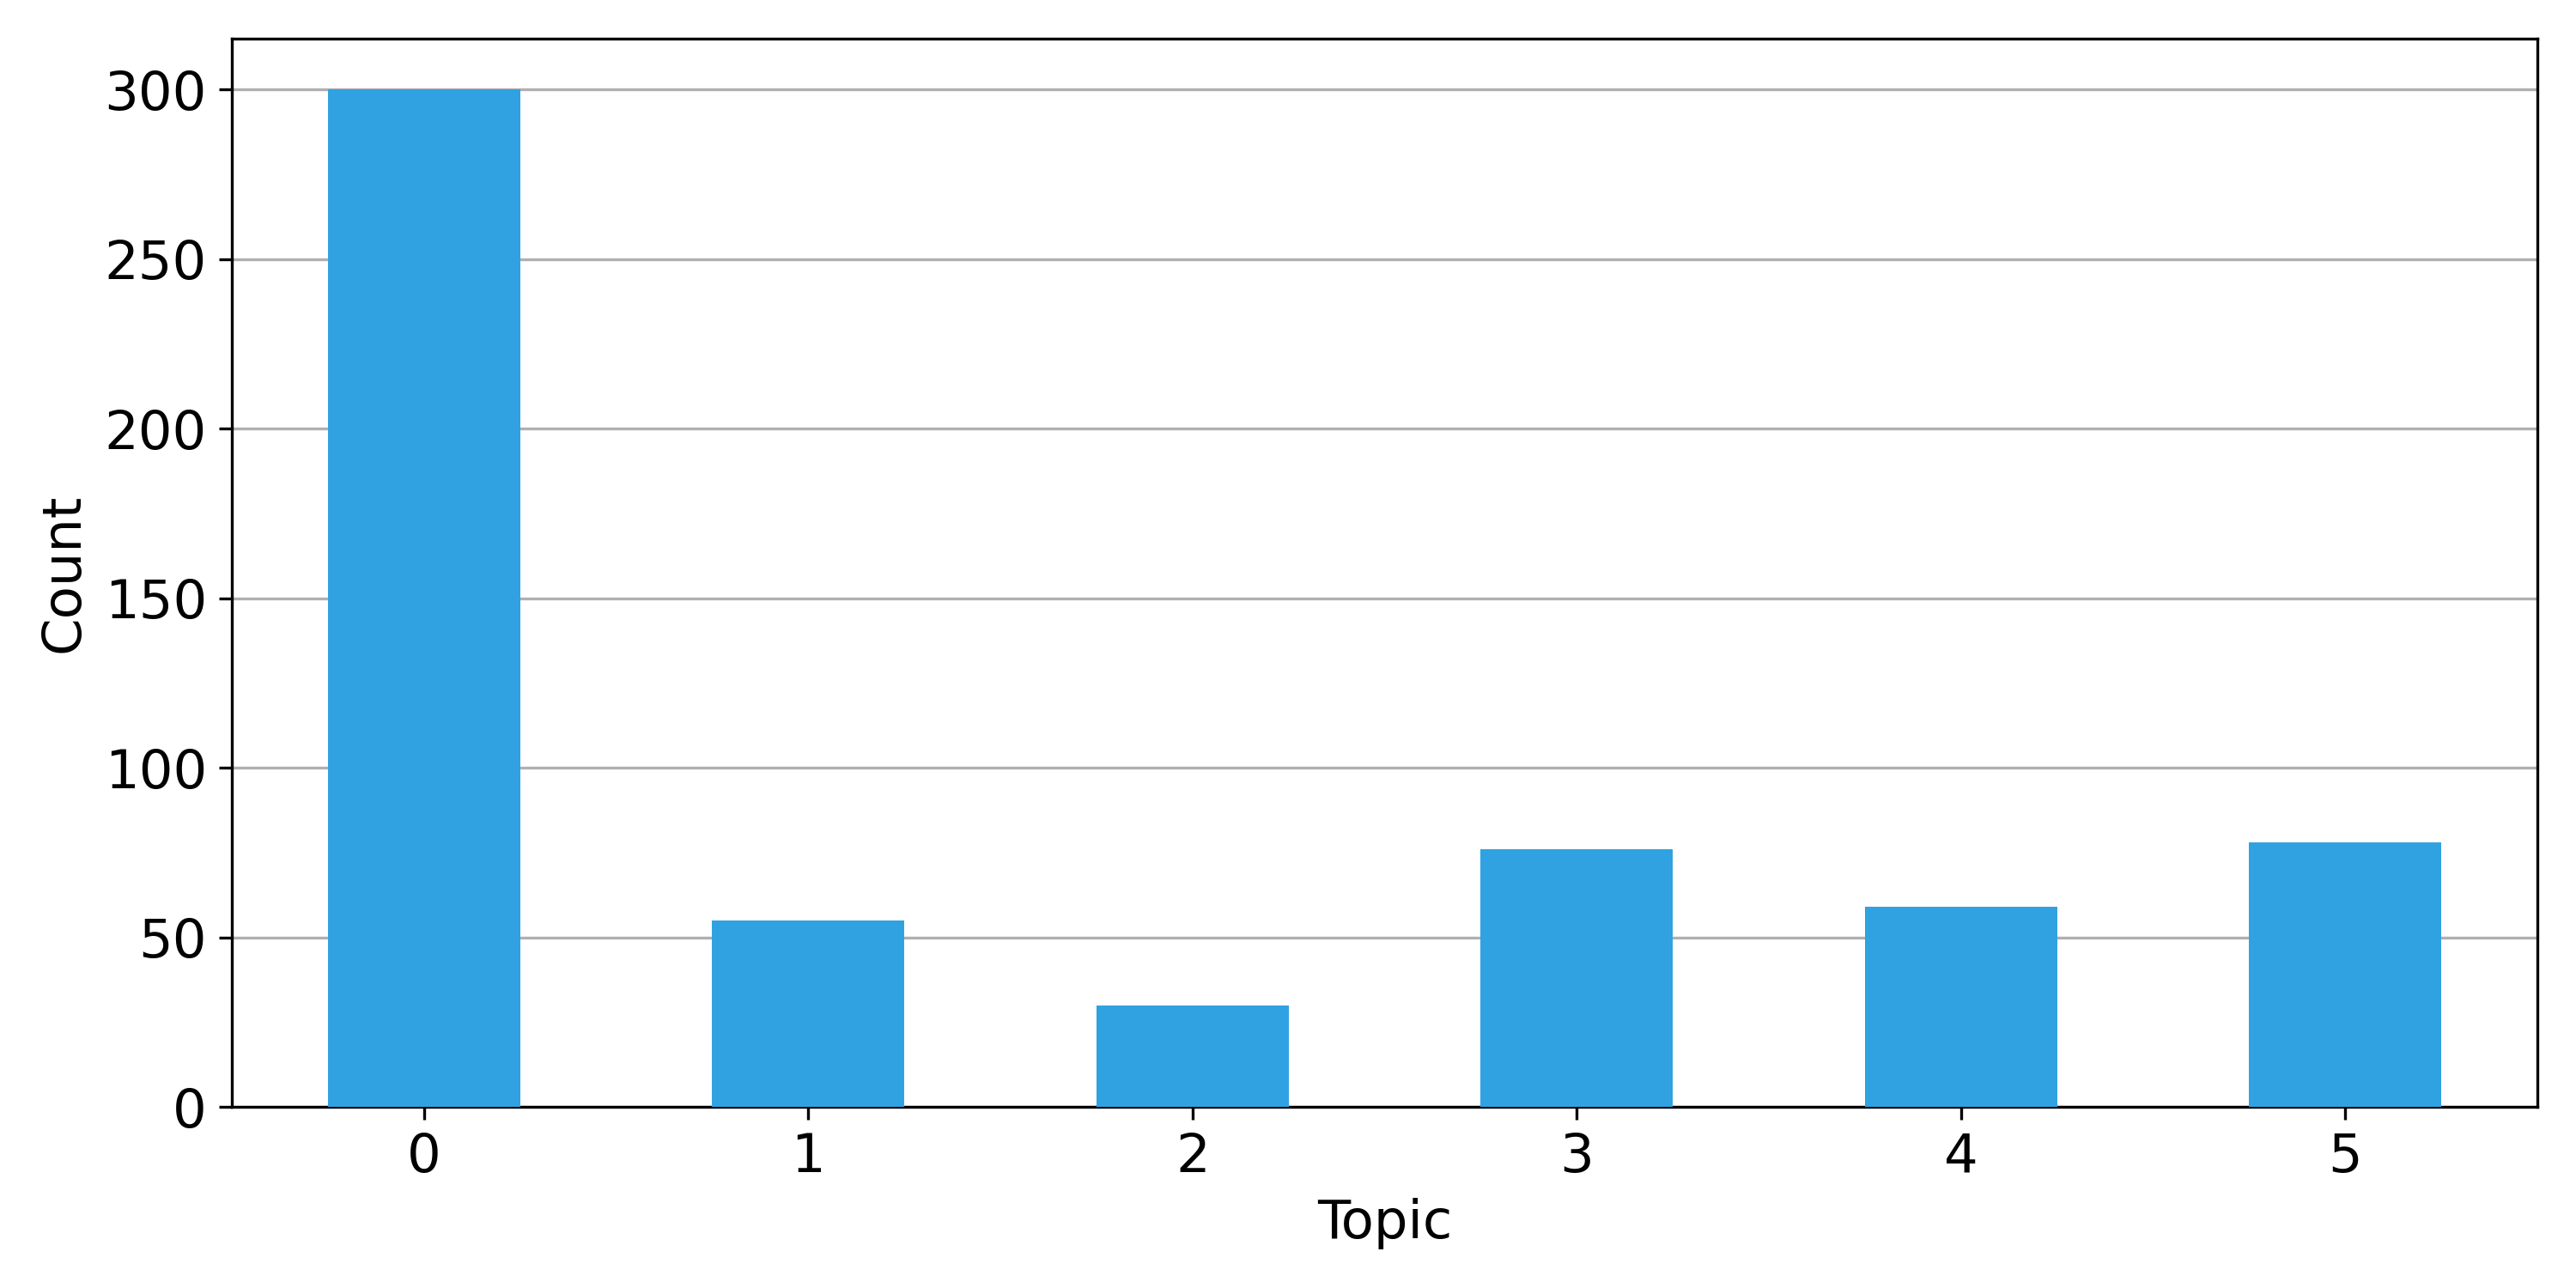
\includegraphics[width=\linewidth]{figures/places_sense_nighttime_locals.png} 
        \caption{Frequency of topics.}
        \label{fig:places_sense_nighttime_locals}
    \end{subfigure}
    \hfill
    \begin{subfigure}{0.5\textwidth}
        \centering
        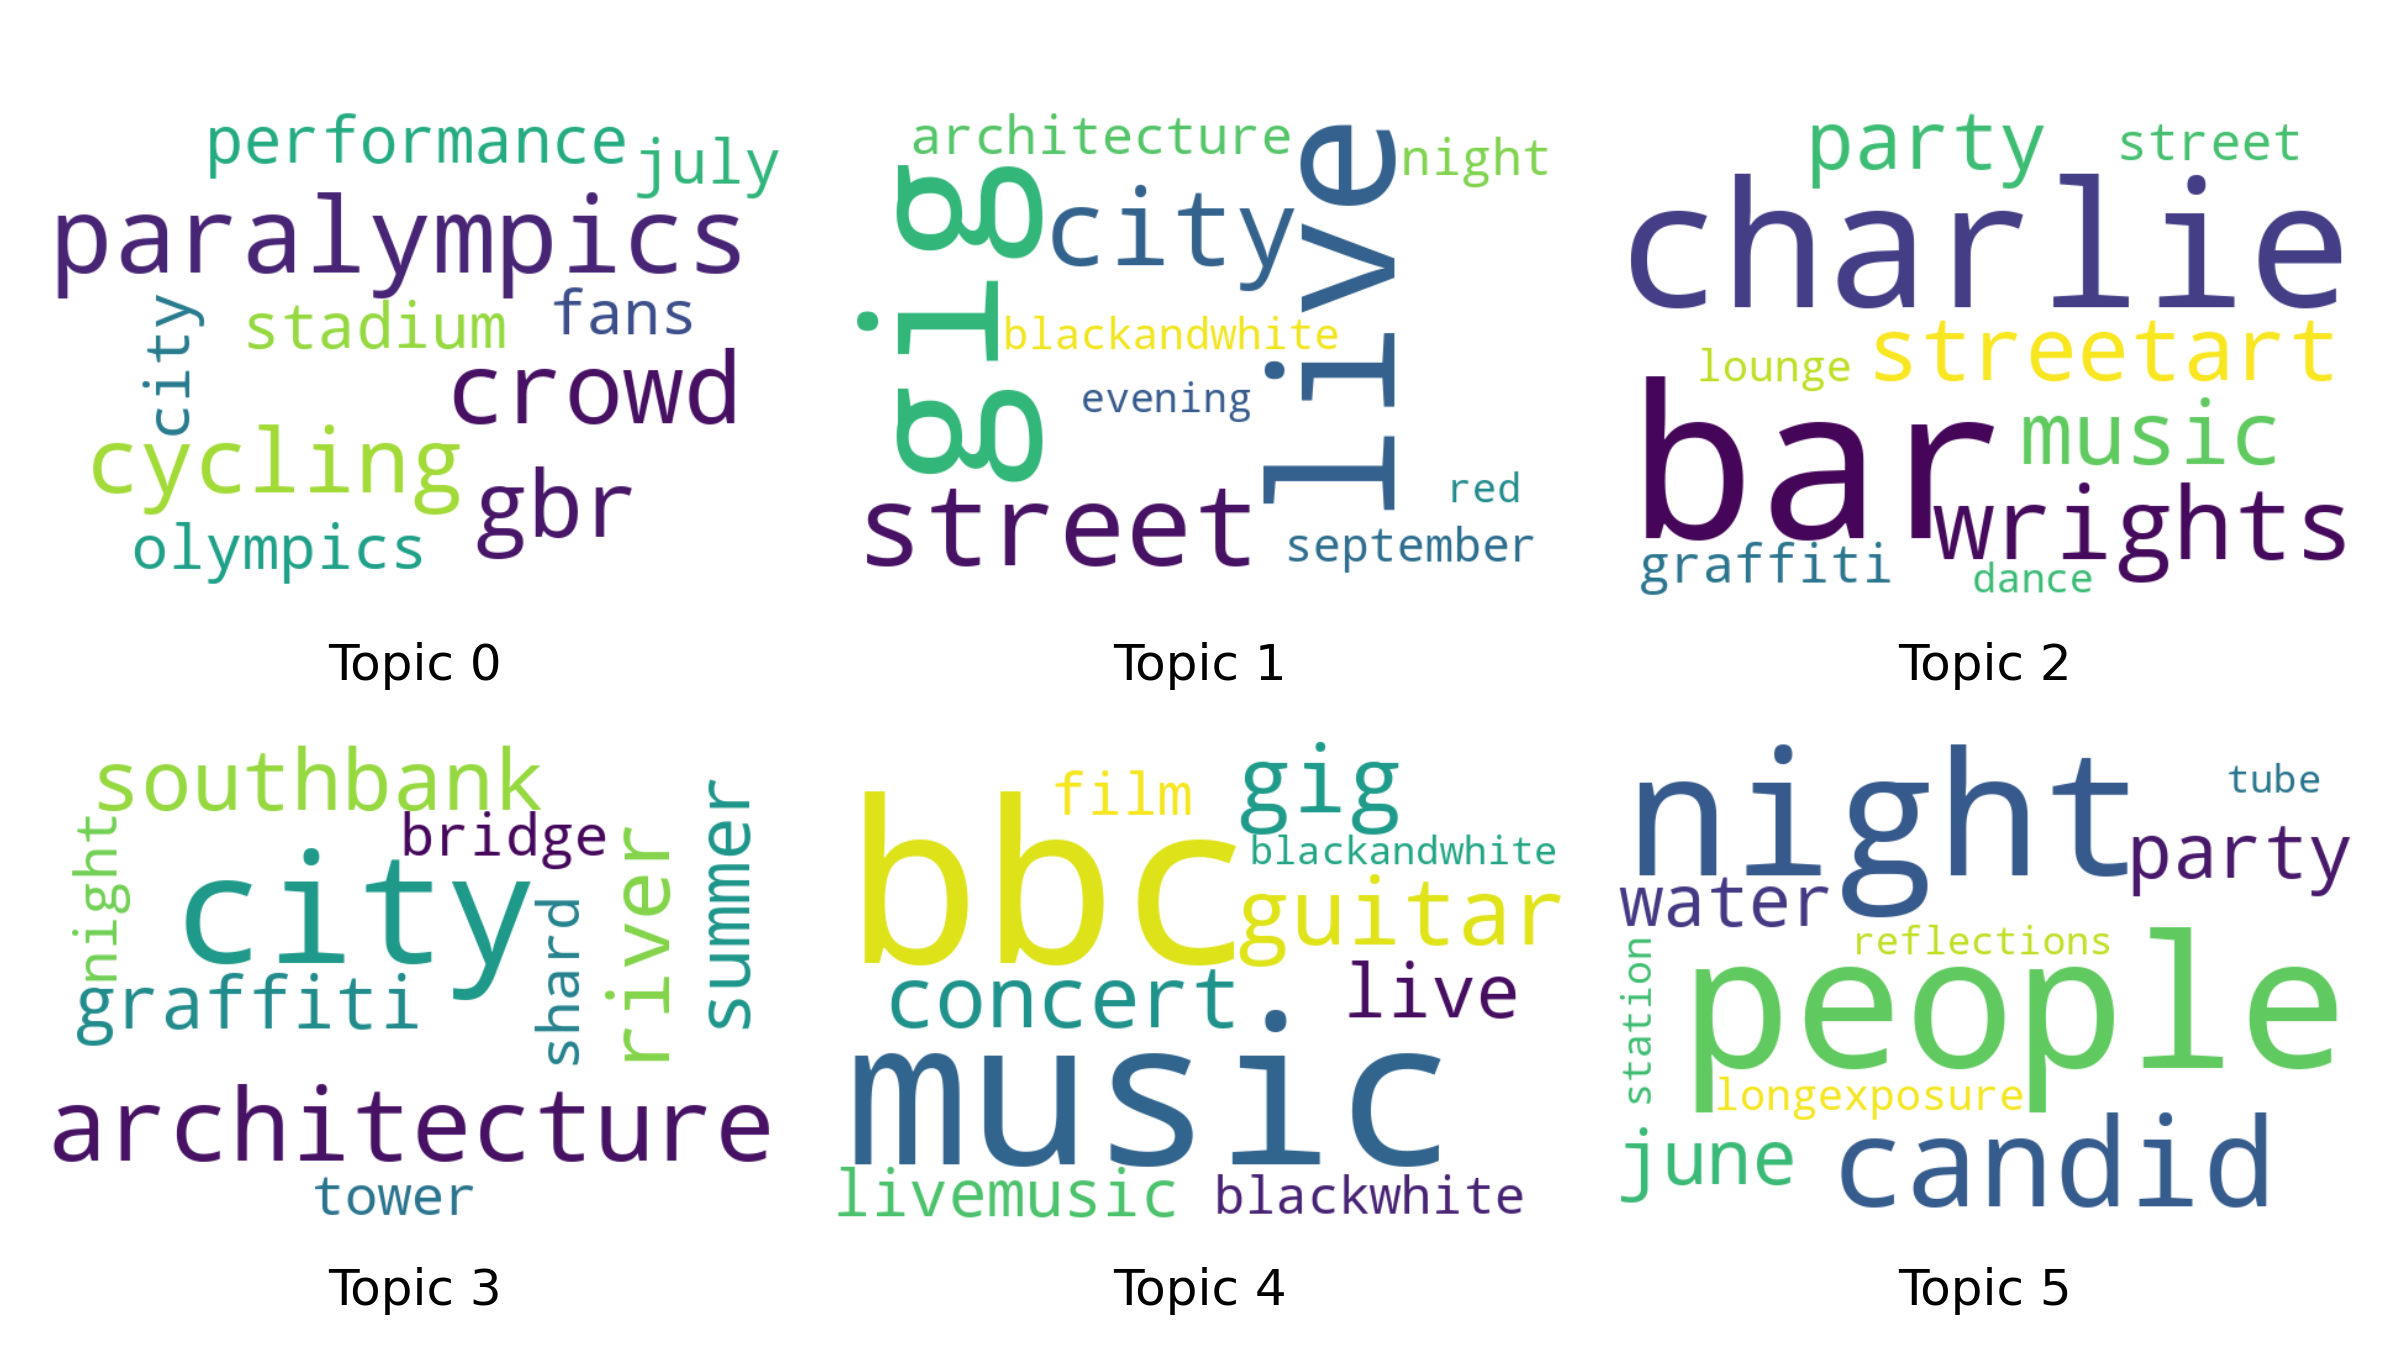
\includegraphics[width=\linewidth]{figures/topics_nighttime_locals.png} 
        \caption{Word clouds for topics.}
        \label{fig:topics_nighttime_locals}
    \end{subfigure}
    
    \begin{subfigure}{0.9\textwidth}
        \centering
        \includegraphics[width=\linewidth]{figures/topics_distribution_nighttime_locals.png} 
        \caption{Distribution of topics.}
        \label{fig:topics_distribution_nighttime_locals}
    \end{subfigure}

    \caption{Sense of place dimension of locals' places during the nighttime.}
    \label{fig:places_topics_sense_locals_nighttime}
\end{figure}

% nighttime tourists
Five topics are generated for tourists in the \textit{Sense of Place} dimension during nighttime hours(Figure~\ref{fig:places_topics_sense_tourists_nighttime}). Similar to locals, tourists at this time also use words related to nighttime activities to describe London, reflected by the emergence of Topic 1 (e.g., concert, live, gig, music) and Topic 4 (e.g., nighttime, city). Compared to the daytime, although the number of places visited by tourists decreases, there is relatively increased interest in places related to museums and transportation, as evidenced by the prominence of Topic 0 (e.g., museum, lhr, station, railway) (Figure~\ref{fig:places_sense_nighttime_tourists}, Figure~\ref{fig:topics_nighttime_tourists}). The distribution of topics is displayed in Figure~\ref{fig:topics_distribution_nighttime_tourists}. While both locals and tourists visit places related to gigs and live music, tourists prefer places around Shoreditch rather than Westminster, as indicated by the distribution Topic 1. Similar to locals, tourists also enjoy visiting places near bridges along the River Thames, which is evidenced by Topic 2 (e.g., architecture, bridge, night, city).

\begin{figure}[!h]
    \centering
    \begin{subfigure}{0.45\textwidth}
        \centering
        \includegraphics[width=\linewidth]{figures/places_sense_nighttime_tourists.png} 
        \caption{Frequency of topics.}
        \label{fig:places_sense_nighttime_tourists}
    \end{subfigure}
    \hfill
    \begin{subfigure}{0.5\textwidth}
        \centering
        \includegraphics[width=\linewidth]{figures/topics_nighttime_tourists.png} 
        \caption{Word clouds for topics.}
        \label{fig:topics_nighttime_tourists}
    \end{subfigure}
    
    \begin{subfigure}{0.9\textwidth}
        \centering
        \includegraphics[width=\linewidth]{figures/topics_distribution_nighttime_tourists.png} 
        \caption{Distribution of topics.}
        \label{fig:topics_distribution_nighttime_tourists}
    \end{subfigure}

    \caption{Sense of place dimension of tourists' places during the nighttime.}
    \label{fig:places_topics_sense_tourists_nighttime}
\end{figure}

% ============== Weekday vs. Weekend ==============
\subsubsubsection{Weekday vs. Weekend}

\textbf{Location}

The distribution of places in the \textit{Location} dimension throughout the week is presented in Figure~\ref{fig:places_location_week}. Generally, boroughs on weekends experience a decrease in the number of places, while the relative relationships of boroughs remain consistent, with Westminster and Camden being the most popular boroughs among locals and tourists throughout the entire week. It is noteworthy that most boroughs are more frequently visited by locals, but Westminster and Hillingdon attract more tourists to visit. Westminster, located in central London, boasts numerous tourist attractions and iconic architecture, making them appealing to tourists. Hillingdon, though situated on the outskirts of London, is home to Heathrow Airport, which draws a large number of tourists to visit. The distribution of the \textit{Location} dimension provides valuable insights into the spatial patterns of places across different boroughs, which highlights the concentration of places in central boroughs and the varying preferences of locals and tourists across different parts of London.

\begin{figure}[!h]

\centering
\begin{subfigure}{0.6\textheight}
\centering
\includegraphics[width=0.9\linewidth]{figures/places_location_weekday.png}
\caption{Weekday.}
\label{fig:places_location_weekday}
\end{subfigure}
\begin{subfigure}{0.6\textheight}
\centering
\includegraphics[width=0.9\linewidth]{figures/places_location_weekend.png}
\caption{Weekend.}
\label{fig:places_location_weekend}
\end{subfigure}

\caption{Location dimension of places on weekdays and weekends.}
\label{fig:places_location_week}
\end{figure}


\textbf{Locale}

The distribution of the \textit{Locale} dimension throughout the week is displayed in Figure~\ref{fig:places_locale_week}. On weekdays, restaurants are more popular than other categories among locals and tourists, followed by professional places, entertainment places, shopping places, and transportation places. Most categories have more places visited by locals, except for the accommodation category as tourists need to find hotels to stay overnight. The popular categories on weekends remain consistent with those on weekdays, with restaurants, entertainment places, shopping places, and transportation places retaining their popularity. However, professional places experience a decrease in visitation. And similar to weekdays, tourists on weekends tend to visit a relatively higher number of places in the accommodation category than locals.


\begin{figure}[!h]

\centering
\begin{subfigure}{0.6\textheight}
\centering
\includegraphics[width=0.9\linewidth]{figures/places_locale_weekday.png}
\caption{Weekday.}
\label{fig:places_locale_weekday}
\end{subfigure}
\begin{subfigure}{0.6\textheight}
\centering
\includegraphics[width=0.9\linewidth]{figures/places_locale_weekend.png}
\caption{Weekend.}
\label{fig:places_locale_weekend}
\end{subfigure}

\caption{Locale dimension of places on weekdays and weekends.}
\label{fig:places_locale_week}
\end{figure}



\textbf{Sense of Place}

% weekday locals
The distribution of \textit{Sense of Place} dimension of locals on weekdays is illustrated in Figure~\ref{fig:places_topics_sense_locals_weekday}. The places visited by locals can be categorized into five topics with three themes: urban life (Topic 0), entertainment (Topic 1), and cityscape (Topic 2, Topic 3, Topic 4). Topic 0 stands out with nearly 700 associated places, while the other four topics contain around 200 places each (Figure~\ref{fig:places_sense_weekday_locals}, Figure~\ref{fig:topics_weekday_locals}). The distribution of topics on weekends in Figure~\ref{fig:topics_distribution_weekday_locals} reveals that words like architecture and buildings (Topic 0) are frequently used to describe various areas in London, which also aligns with patterns observed in other time spans. In addition, central boroughs, such as Lambeth, Kensington and Chelsea, Westminster, Camden, and the City of London, can be described by words like live, gig, and southbank, as illustrated in Topic 1. In terms of topics related to the cityscape, the inner part of London can be characterized by graffiti, street art, river, and city (Topic 2, Topic 4), whereas Topic 3 (e.g., bus, people) contains more general words, which also covers outer London.

\begin{figure}[!h]
    \centering
    \begin{subfigure}{0.45\textwidth}
        \centering
        \includegraphics[width=\linewidth]{figures/places_sense_weekday_locals.png} 
        \caption{Frequency of topics.}
        \label{fig:places_sense_weekday_locals}
    \end{subfigure}
    \hfill
    \begin{subfigure}{0.5\textwidth}
        \centering
        \includegraphics[width=\linewidth]{figures/topics_weekday_locals.png} 
        \caption{Word clouds for topics.}
        \label{fig:topics_weekday_locals}
    \end{subfigure}
    
    \begin{subfigure}{0.9\textwidth}
        \centering
        \includegraphics[width=\linewidth]{figures/topics_distribution_weekday_locals.png} 
        \caption{Distribution of topics.}
        \label{fig:topics_distribution_weekday_locals}
    \end{subfigure}

    \caption{Sense of place dimension of locals' places during the weekday.}
    \label{fig:places_topics_sense_locals_weekday}
\end{figure}

% weekday tourist
The weekday distribution of tourists' places in the \textit{Sense of Place} dimension is displayed in Figure~\ref{fig:places_topics_sense_tourists_weekday}. Tourists tend to visit places associated with the Olympics (Topic 0) and cityscape (Topic 5), with each topic comprising approximately 250 places. Tourists also like to visit places related to transport, art, and tourist attractions, as evidenced by the high occurrence of Topic 1 (e.g., museum, victoria, station, art) and Topic 3 (e.g., architecture, bridge, shard), both featuring over 150 associated places (Figure~\ref{fig:places_sense_weekday_tourists}, Figure~\ref{fig:topics_weekday_tourists}). The distribution of topics on weekdays in Figure~\ref{fig:topics_distribution_weekday_locals} suggests that the inner part of London attracts the most descriptions from tourists, including topics related to the Olympics, cityscape, transportation, and art. Furthermore, the area surrounding Heathrow Airport leaves a strong impression on tourists, as indicated by a concentration of places in Topic 4 (e.g., lhr, airbus, boeing) in that region.

\begin{figure}[!h]
    \centering
    \begin{subfigure}{0.45\textwidth}
        \centering
        \includegraphics[width=\linewidth]{figures/places_sense_weekday_tourists.png} 
        \caption{Frequency of topics.}
        \label{fig:places_sense_weekday_tourists}
    \end{subfigure}
    \hfill
    \begin{subfigure}{0.5\textwidth}
        \centering
        \includegraphics[width=\linewidth]{figures/topics_weekday_tourists.png} 
        \caption{Word clouds for topics.}
        \label{fig:topics_weekday_tourists}
    \end{subfigure}
    
    \begin{subfigure}{0.9\textwidth}
        \centering
        \includegraphics[width=\linewidth]{figures/topics_distribution_weekday_tourists.png} 
        \caption{Distribution of topics.}
        \label{fig:topics_distribution_weekday_tourists}
    \end{subfigure}

    \caption{Sense of place dimension of tourists' places during the weekday.}
    \label{fig:places_topics_sense_tourists_weekday}
\end{figure}

% weekend locals
On weekends, locals' descriptions are summarized by six topics (Figure~\ref{fig:places_topics_sense_locals_weekend}). 
In addition to the places known for graffiti and street art in Topic 1, which are consistently popular throughout different time spans, locals demonstrate a preference for more nature-related locations compared to weekdays. This preference is evident in the popularity of Topic 0, which includes words like park and garden, and encompasses approximately 250 associated places. Additionally, locals on weekends tend to explore sports-related places represented by Topic 4 (e.g., city, gbr, football, race) and Topic 5 (e.g., paralympics, olympics) (Figure~\ref{fig:places_sense_weekend_locals}, Figure~\ref{fig:topics_weekend_locals}). The places in Topic 0 and Topic 1 are scattered across London, as parks and graffiti can be found throughout the city. Regarding the areas that are described by locals with sports-related topics, the vicinity of sports venues like Emirates Stadium (a football stadium) and London Stadium are concentrated with places in Topic 4 and Topic 5 (Figure~\ref{fig:topics_distribution_weekend_locals}).

\begin{figure}[!h]
    \centering
    \begin{subfigure}{0.45\textwidth}
        \centering
        \includegraphics[width=\linewidth]{figures/places_sense_weekend_locals.png} 
        \caption{Frequency of topics.}
        \label{fig:places_sense_weekend_locals}
    \end{subfigure}
    \hfill
    \begin{subfigure}{0.5\textwidth}
        \centering
        \includegraphics[width=\linewidth]{figures/topics_weekend_locals.png} 
        \caption{Word clouds for topics.}
        \label{fig:topics_weekend_locals}
    \end{subfigure}
    
    \begin{subfigure}{0.9\textwidth}
        \centering
        \includegraphics[width=\linewidth]{figures/topics_distribution_weekend_locals.png} 
        \caption{Distribution of topics.}
        \label{fig:topics_distribution_weekend_locals}
    \end{subfigure}

    \caption{Sense of place dimension of locals' places during the weekend.}
    \label{fig:places_topics_sense_locals_weekend}
\end{figure}

% weekend tourist
Tourists' descriptions of the city on weekends are generalized with six topics (Figure~\ref{fig:places_topics_sense_tourists_weekend}). Tourists continue to visit places characterized by architecture, street art, and transport at this time span, which is similar to their choices on weekdays. Over 250 places visited by tourists are described with Topic 0 (e.g., marathon, city, architecture). And similar to locals' descriptions on weekdays, tourists also tend to visit places featured with graffiti and street art, as indicated by the popularity of Topic 1 (Figure~\ref{fig:places_sense_weekend_tourists}, Figure~\ref{fig:topics_weekend_tourists}). Concerning the distribution of places across various topics, except for places linked to Topic 0 which are distributed throughout London with a concentration in the city center, Topic 1, Topic 3 (e.g., olympics, gbr, park), and Topic 5 (e.g., city, architecture, bridge) are predominantly located in the inner part of London Figure~\ref{fig:places_topics_sense_tourists_weekend}).

\begin{figure}[!h]
    \centering
    \begin{subfigure}{0.45\textwidth}
        \centering
        \includegraphics[width=\linewidth]{figures/places_sense_weekend_tourists.png} 
        \caption{Frequency of topics.}
        \label{fig:places_sense_weekend_tourists}
    \end{subfigure}
    \hfill
    \begin{subfigure}{0.5\textwidth}
        \centering
        \includegraphics[width=\linewidth]{figures/topics_weekend_tourists.png} 
        \caption{Word clouds for topics.}
        \label{fig:topics_weekend_tourists}
    \end{subfigure}
    
    \begin{subfigure}{0.9\textwidth}
        \centering
        \includegraphics[width=\linewidth]{figures/topics_distribution_weekend_tourists.png} 
        \caption{Distribution of topics.}
        \label{fig:topics_distribution_weekend_tourists}
    \end{subfigure}

    \caption{Sense of place dimension of tourists' places during the weekend.}
    \label{fig:places_topics_sense_tourists_weekend}
\end{figure}


% ============================= || Spatiotemporal Patterns of Semantic Trajectory || =============================
\subsection{Spatiotemporal Patterns of Semantic Trajectory} \label{patterns_traj}
To gain insights into how locals and tourists perceive the city along their trajectories at different time spans, semantic trajectories were constructed for various scenes, such as locals during the daytime and tourists on weekdays. The number of trajectories for each scene is summarized in Table~\ref{tab:trajectories_summary}. While the number of locals is lower than that of tourists, both groups generate a similar number of trajectories. A total of 1,460 trajectories are generated by locals and tourists during the daytime, significantly more than the 121 trajectories during the nighttime. Similarly, the number of trajectories on weekdays (1,240) surpasses those on weekends (490). In order to delve into a more precise understanding of city perception through semantic trajectories, Section \ref{perception_through_traj} will analyze the trajectory distribution and the frequency of semantic dimensions across different time spans. Furthermore, Section \ref{comparison_perception} will conduct a comparative analysis of semantic trajectories, enabling exploration of the dynamic nature of city perception.

\begin{table}[h!]
\centering
\caption{\label{tab:trajectories_summary}Summary of trajectories.}
\begin{tabular}{llll} \hline
Time & Population group & No. of users & No. of trajectories \\
\hline
\multirow{3}{*}{Daytime} 
& All Users & 6,919 & 1,460 \\
& Locals & 1,077 & 784 \\
& Tourists & 5,842 & 676 \\
\hline
\multirow{3}{*}{Nighttime} 
& All Users & 4,425 & 121 \\
& Locals & 996 & 63 \\
& Tourists & 3,429 & 58 \\
\hline
\multirow{3}{*}{Weekday} 
& All Users & 6,497 & 1,240 \\
& Locals & 1,069 & 659 \\
& Tourists & 5,428 & 581 \\
\hline
\multirow{3}{*}{Weekend} 
& All Users & 4,886 & 490 \\
& Locals & 1,011 & 213 \\
& Tourists & 3,875 & 277 \\
\hline
\end{tabular}
\end{table}

% ====================== | City Perception through Semantic Trajectory | ======================
\subsubsection{City Perception through Semantic Trajectory} \label{perception_through_traj}

\subsubsubsection{Daytime}

% daytime locals
Figure~\ref{fig:traj_distribution_daytime_locals} shows the five trajectory clusters of locals during the daytime, with their typical trajectories highlighted in dark red. The majority of locals tend to move within the city center, as evidenced by the high visitation frequency of Westminster, Camden, and the City of London in the \textit{Location} dimension, as shown in Figure~\ref{fig:traj_location_daytime_locals}. Some locals also visit the south of Greenwich from the city center, particularly around the Coldharbour Leisure Center, which offers a range of sports facilities. Another noteworthy trajectory pattern is observed between central London and the outskirts boroughs, although the frequency of these outer boroughs is significantly lower compared to the inner ones. In terms of the \textit{Locale} dimension, trajectories in most clusters predominantly pass through places related to transportation, shopping, restaurants, and professional activities. Notably, entertainment places and green \& blue spaces are also frequently visited by trajectories in Cluster 0 and Cluster 4 (Figure~\ref{fig:traj_locale_daytime_locals}). The \textit{Sense of Place} dimension in Figure~\ref{fig:traj_sense_daytime_locals} provides insights into how locals describe the city along their trajectories during the daytime, and the word clouds of topics are displayed in Figure~\ref{fig:topics_daytime_locals}. Trajectories in Cluster 0 and Cluster 4 often encompass tags associated with transportation and nature, such as parks and rivers (Topic 1, and Topic 4), indicating that these clusters revolve around nature sightseeing. Cluster 0 and Cluster 1 suggest that locals tend to visit the south of Greenwich from the city center, particularly around the Coldharbour Leisure Center, which offers a range of sports facilities. Cluster 1 and Cluster 2 have some typical trajectories that are air transport-oriented, as these trajectories associated with these clusters are primarily characterized by Topic 0 (e.g., lhr, airbus), with typical trajectories connecting central London and the vicinity of Heathrow Airport, particularly in Islington and Hounslow. Cluster 3 is characterized by trajectories primarily focused on work-related purposes, as they frequently visit professional places and restaurants. Moreover, the typical trajectories in this cluster predominantly link the city center with Merton and Wandsworth, which are residential districts.

\begin{figure}[!h]
\centering
\includegraphics[width=1\textwidth]{figures/traj_distribution_daytime_locals.png}
\caption{\label{fig:traj_distribution_daytime_locals}Distribution of locals' trajectories during the daytime (typical trajectories are represented by the dark red color).}
\end{figure}


\begin{figure}[!h]

\centering
\begin{subfigure}{0.6\textheight}
\centering
\includegraphics[width=1\linewidth]{figures/traj_location_daytime_locals.png}
\caption{Location.}
\label{fig:traj_location_daytime_locals}
\end{subfigure}
\begin{subfigure}{0.6\textheight}
\centering
\includegraphics[width=1\linewidth]{figures/traj_locale_daytime_locals.png}
\caption{Locale.}
\label{fig:traj_locale_daytime_locals}
\end{subfigure}
\begin{subfigure}{0.6\textheight}
\centering
\includegraphics[width=1\linewidth]{figures/traj_sense_daytime_locals.png}
\caption{Sense of Place.}
\label{fig:traj_sense_daytime_locals}
\end{subfigure}

\caption{Trajectory dimensions of locals during the daytime.}
\label{fig:traj_dimension_daytime_locas}
\end{figure}


% daytime tourists
Trajectories of tourists during the nighttime are clustered into four groups based on their semantic dimensions, and compared with locals, tourists also exhibit a similar movement pattern within the city center during the daytime, with additional trajectories that connect the outer and inner parts of London, as illustrated in Figure~\ref{fig:traj_distribution_daytime_tourists}. Figure~\ref{fig:traj_dimension_daytime_tourists} shows the frequency of dimensions in the semantic trajectories of tourists during the daytime. In terms of the \textit{Location} dimension, inner boroughs are popular among tourists, such as Westminster and Camden, and Kensington and Chelsea. In the \textit{Locale} dimension, in addition to the categories that attract both locals and tourists, such as transportation, professional places, restaurants, and shopping places, tourists also demonstrate an interest in art places and entertainment places, particularly those generating trajectories in Cluster 3. As for the \textit{Sense of Place} dimension, both locals and tourists use similar words to describe the places they visit, with a focus on transportation and cityscapes, such as bus and street. Tourists also frequently mention places associated with the Olympics (word clouds of topics are displayed in Figure~\ref{fig:topics_daytime_tourists}). The typical trajectories of each cluster are represented in dark red in Figure~\ref{fig:traj_distribution_daytime_tourists}, for more detailed distributions, please refer to Figure~\ref{fig:sequences_daytime_tourists} in Appendix \ref{appendix}. Cluster 0 and Cluster 1 are transportation-related as their typical trajectories primarily link the transportation hubs in central London, such as Stratford Station, King's Cross, and Waterloo Station. Cluster 1 also exhibits typical trajectories connecting the city center and outer boroughs like Croydon and Merton. Cluster 2 is associated with shopping as it demonstrates a high frequency of shopping places in the \textit{Locale} dimension, and its typical trajectories extend along Oxford Street, a renowned shopping street in London. Trajectories in Cluster 3 feature a substantial number of art places and entertainment places, and the typical trajectories passing through various tourist attractions and museums in Westminster, such as Trafalgar Square, Big Ben, and Victoria and Albert Museum. Thus, this cluster can be interpreted as representing the sightseeing routes for tourists.

\begin{figure}[!h]
\centering
\includegraphics[width=1\textwidth]{figures/traj_distribution_daytime_tourists.png}
\caption{\label{fig:traj_distribution_daytime_tourists}Distribution of tourists' trajectories during the daytime (typical trajectories are represented by the dark red color).}
\end{figure}


\begin{figure}[!h]

\centering
\begin{subfigure}{0.6\textheight}
\centering
\includegraphics[width=1\linewidth]{figures/traj_location_daytime_tourists.png}
\caption{Location.}
\label{fig:traj_location_daytime_tourists}
\end{subfigure}
\begin{subfigure}{0.6\textheight}
\centering
\includegraphics[width=1\linewidth]{figures/traj_locale_daytime_tourists.png}
\caption{Locale.}
\label{fig:traj_locale_daytime_tourists}
\end{subfigure}
\begin{subfigure}{0.6\textheight}
\centering
\includegraphics[width=1\linewidth]{figures/traj_sense_daytime_tourists.png}
\caption{Sense of Place.}
\label{fig:traj_sense_daytime_tourists}
\end{subfigure}

\caption{Trajectory dimensions of tourists during the daytime.}
\label{fig:traj_dimension_daytime_tourists}
\end{figure}

\subsubsubsection{Nighttime}

% nighttime locals
When it comes to nighttime, locals generate a smaller number of trajectories, which are clustered into three groups. Locals have lower activity density in the city center during this period, but they display stronger connections with outskirts boroughs that have large residential districts, such as Merton, and Croydon (Figure~\ref{fig:traj_distribution_nighttime_locals}). In terms of the distribution of semantic dimensions in their trajectories, apart from Westminster, which remains one of the most popular boroughs, Greenwich is also frequently visited by trajectories from all three clusters in the \textit{Location} dimension (Figure~\ref{fig:traj_location_nighttime_locals}). transportation places, shopping places, restaurants, and professional places continue to be the most frequently visited places throughout the day in the \textit{Locale} dimension. Notably, locals also tend to visit green \& blue spaces during the nighttime (Figure~\ref{fig:traj_locale_nighttime_locals}). In the \textit{Sense of Place} dimension, the descriptions provided by locals regarding the city shift from nature and transportation related aspects to leisure and sports activities during the nighttime. This shift is reflected in the higher frequency of Topic 0 (e.g., paralympics, cycling, crowd), Topic 3 (e.g., city, architecture, southbank), and Topic 4 (e.g., music, bbc, concert, gig) (Figure~\ref{fig:traj_sense_nighttime_locals}, Figure~\ref{fig:topics_nighttime_locals}). Similar to the daytime, locals also have their typical trajectories connecting transportation hubs. This is evidenced by the link between Ealing Broadway Station in Ealing and King's Cross in Islington in cluster 0. It is important to highlight that the typical trajectories of all three clusters pass through the southern part of Greenwich during the nighttime. This area is home to the Coldharbour Leisure Center and Mottingham Sports Ground/Foxes Fields, which offer numerous sports facilities (Figure~\ref{fig:sequences_nighttime_locals}). It can be concluded that locals during the nighttime are not concentrated in the city center, instead, they tend to visit Greenwich for fitness exercises. Moreover, locals' perceptions of the city are more focused on nighttime leisure activities, such as gig and live music.

\begin{figure}[!h]
\centering
\includegraphics[width=1\textwidth]{figures/traj_distribution_nighttime_locals.png}
\caption{\label{fig:traj_distribution_nighttime_locals}Distribution of locals' trajectories during the nighttime (typical trajectories are represented by the dark red color).}
\end{figure}


\begin{figure}[!h]

\centering
\begin{subfigure}{0.6\textheight}
\centering
\includegraphics[width=1\linewidth]{figures/traj_location_nighttime_locals.png}
\caption{Location.}
\label{fig:traj_location_nighttime_locals}
\end{subfigure}
\begin{subfigure}{0.6\textheight}
\centering
\includegraphics[width=1\linewidth]{figures/traj_locale_nighttime_locals.png}
\caption{Locale.}
\label{fig:traj_locale_nighttime_locals}
\end{subfigure}
\begin{subfigure}{0.6\textheight}
\centering
\includegraphics[width=1\linewidth]{figures/traj_sense_nighttime_locals.png}
\caption{Sense of Place.}
\label{fig:traj_sense_nighttime_locals}
\end{subfigure}

\caption{Trajectory dimensions of locals during the nighttime.}
\label{fig:traj_dimension_nighttime_locas}
\end{figure}


% nighttime tourists
Trajectories of tourists during the nighttime are clustered into two groups. In comparison to locals, tourists during the nighttime tend to concentrate their movement within the city center, with fewer trajectories visiting outskirts boroughs (Figure~\ref{fig:traj_distribution_nighttime_tourists}). In addition to Westminster and Camden, tourists also exhibit interest in Tower Hamlets and Hackney in the \textit{Location} dimension (Figure~\ref{fig:traj_location_nighttime_tourists}). While both locals and tourists frequently visit transportation places, shopping places, restaurants, and professional places during the nighttime, tourists display a higher inclination towards art places and entertainment places rather than green \& blue spaces (Figure~\ref{fig:traj_locale_nighttime_tourists}). Regarding the \textit{Sense of Place} dimension, tourists tend to use more general words to describe London during the nighttime, such as city, street, and night. Additionally, words associated with art and transportation, such as museum, station, and railway, are also frequently mentioned. This is reflected in the high frequency of Topic 0 and Topic 4 (Figure~\ref{fig:traj_sense_nighttime_tourists}, Figure~\ref{fig:topics_nighttime_tourists}). The typical trajectories of tourists during the nighttime exhibit distinct patterns compared to those of locals. These trajectories primarily connect shopping and entertainment places in the inner part of London. Specifically, they encompass places such as the Stratford Shopping Center in Newham, Shoreditch in Hackney, and renowned squares and streets in Westminster, including Piccadilly Circus, Leicester Square, and Oxford Street (Figure~\ref{fig:sequences_nighttime_tourists}). In summary, tourists display lower nighttime activity levels with fewer trajectories but maintain a consistent interest in vibrant areas for shopping and entertainment throughout the day.

\begin{figure}[!h]
\centering
\includegraphics[width=1\textwidth]{figures/traj_distribution_nighttime_tourists.png}
\caption{\label{fig:traj_distribution_nighttime_tourists}Distribution of tourists' trajectories during the nighttime (typical trajectories are represented by the dark red color).}
\end{figure}


\begin{figure}[!h]

\centering
\begin{subfigure}{0.6\textheight}
\centering
\includegraphics[width=1\linewidth]{figures/traj_location_nighttime_tourists.png}
\caption{Location.}
\label{fig:traj_location_nighttime_tourists}
\end{subfigure}
\begin{subfigure}{0.6\textheight}
\centering
\includegraphics[width=1\linewidth]{figures/traj_locale_nighttime_tourists.png}
\caption{Locale.}
\label{fig:traj_locale_nighttime_tourists}
\end{subfigure}
\begin{subfigure}{0.6\textheight}
\centering
\includegraphics[width=1\linewidth]{figures/traj_sense_nighttime_tourists.png}
\caption{Sense of Place.}
\label{fig:traj_sense_nighttime_tourists}
\end{subfigure}

\caption{Trajectory dimensions of tourists during the nighttime.}
\label{fig:traj_dimension_nighttime_tourists}
\end{figure}


\subsubsubsection{Weekday}

% weekday locals
Trajectories of locals on weekdays are divided into five clusters and these clusters cover both the inner and outer parts of London  (Figure~\ref{fig:traj_distribution_weekday_locals}). The frequency of trajectories in the \textit{Location} dimension is illustrated in Figure~\ref{fig:traj_location_weekday_locals}. Cluster 0, Cluster 3, and Cluster 4 have trajectories more concentrated in the city center, encompassing boroughs such as Westminster, Camden, and the City of London. Cluster 1 gravitates towards Southwest London, particularly Hillingdon and Hounslow. Cluster 2 is concentrated in Southeast London, with Greenwich being visited at a high frequency. Regarding the \textit{Locale} dimension, transportation places remain the most frequently visited by locals on weekdays, accompanied by shopping places, restaurants, and professional places across all clusters (Figure~\ref{fig:traj_locale_weekday_locals}). In terms of the \textit{Sense of Place} dimension, locals tend to use general words to describe the city. Topic 1 is assigned to a large number of trajectories in all five clusters, and it is about the cityscape like architecture, buildings, and railways. Notably, Cluster 1 contains trajectories with a higher occurrence of Topic 2 (e.g., lhr, airbus), which aligns with its distribution around Heathrow Airport. Furthermore, Cluster 3 has a high frequency in Topic 1 (e.g., live, gig, southbank) and visits more entertainment places compared to other clusters, suggesting a more leisure-oriented focus (Figure~\ref{fig:traj_sense_weekday_locals}, Figure~\ref{fig:topics_weekday_locals}). The typical trajectories of Cluster 0 and Cluster 4 are likely generated by local commuters as they connect outer boroughs with the main transportation hubs in the city center, which are similar to some movement patterns observed among locals during the daytime. Cluster 1 exhibits typical trajectories concentrated around Heathrow Airport and the nearby borough of Hounslow, reflecting a perception of airport-related areas. Cluster 2 displays typical trajectories covering the southern region of Greenwich, indicating its suitability for sports activities due to the presence of numerous sports facilities (Figure~\ref{fig:sequences_weekday_locals}).


\begin{figure}[!h]
\centering
\includegraphics[width=1\textwidth]{figures/traj_distribution_weekday_locals.png}
\caption{\label{fig:traj_distribution_weekday_locals}Distribution of locals' trajectories on weekdays (typical trajectories are represented by the dark red color).}
\end{figure}


\begin{figure}[!h]

\centering
\begin{subfigure}{0.6\textheight}
\centering
\includegraphics[width=1\linewidth]{figures/traj_location_weekday_locals.png}
\caption{Location.}
\label{fig:traj_location_weekday_locals}
\end{subfigure}
\begin{subfigure}{0.6\textheight}
\centering
\includegraphics[width=1\linewidth]{figures/traj_locale_weekday_locals.png}
\caption{Locale.}
\label{fig:traj_locale_weekday_locals}
\end{subfigure}
\begin{subfigure}{0.6\textheight}
\centering
\includegraphics[width=1\linewidth]{figures/traj_sense_weekday_locals.png}
\caption{Sense of Place.}
\label{fig:traj_sense_weekday_locals}
\end{subfigure}

\caption{Trajectory dimensions of locals on weekdays.}
\label{fig:traj_dimension_weekday_locas}
\end{figure}


% weekday tourists
On weekdays, tourists also explore the outer part of London, but unlike locals who tend to gravitate towards particular boroughs, tourists mainly concentrate their movements in central London. Their trajectories are divided into four clusters (Figure~\ref{fig:traj_distribution_weekday_tourists}). The distribution of the \textit{Location} dimension in Figure~\ref{traj_location_weekday_tourists} confirms this finding. Westminster is the most frequently visited borough, followed by Camden and Kensington and Chelsea, all of which are in the city center. In contrast to locals who often visit outskirts boroughs, tourists rarely visit these areas. Tourists also exhibit different preferences in place categories, as revealed by the \textit{Locale} dimension in Figure~\ref{traj_locale_weekday_tourists}. While transportation remains popular in general, trajectories in certain clusters are not primarily comprised of this category but are also characterized by other categories like professional places, shopping places, and restaurants, particularly in Cluster 0 and Cluster 2. In terms of the \textit{Sense of Place} dimension, tourists, similar to locals, also tend to use general words to describe the city, such as street, architecture, and city. However, tourists display a greater interest in art and the Olympics, as indicated by the frequent mention of words like museum, art, and olympics (Figure~\ref{fig:traj_sense_weekday_tourists}, Figure~\ref{fig:topics_weekday_tourists}). Typical trajectories of tourists on weekdays have many similarities to those observed during other time periods. Sightseeing and shopping remain the primary activities within the city center throughout the day, with tourists visiting various attractions, museums, and shopping streets. This pattern persists on weekdays, with tourists also visiting similar places around Stratford Shopping Center, Shoreditch, and Leicester Square (Figure~\ref{fig:sequences_weekday_tourists}).

\begin{figure}[!h]
\centering
\includegraphics[width=1\textwidth]{figures/traj_distribution_weekday_tourists.png}
\caption{\label{fig:traj_distribution_weekday_tourists}Distribution of tourists' trajectories on weekdays (typical trajectories are represented by the dark red color).}
\end{figure}


\begin{figure}[!h]

\centering
\begin{subfigure}{0.6\textheight}
\centering
\includegraphics[width=1\linewidth]{figures/traj_location_weekday_tourists.png}
\caption{Location.}
\label{fig:traj_location_weekday_tourists}
\end{subfigure}
\begin{subfigure}{0.6\textheight}
\centering
\includegraphics[width=1\linewidth]{figures/traj_locale_weekday_tourists.png}
\caption{Locale.}
\label{fig:traj_locale_weekday_tourists}
\end{subfigure}
\begin{subfigure}{0.6\textheight}
\centering
\includegraphics[width=1\linewidth]{figures/traj_sense_weekday_tourists.png}
\caption{Sense of Place.}
\label{fig:traj_sense_weekday_tourists}
\end{subfigure}

\caption{Trajectory dimensions of tourists on weekdays.}
\label{fig:traj_dimension_weekday_tourists}
\end{figure}


\subsubsubsection{Weekend}

% weekend locals
When it comes to weekends, locals are less active, generating a smaller number of trajectories compared to weekdays, although they concentrate their activities in central London, their trajectories become sparser (Figure~\ref{fig:traj_distribution_weekend_locals}). The frequency of the \textit{Location} dimension in Figure~\ref{fig:traj_location_weekend_locals} also suggests that trajectories of tourists are more evenly distributed in inner and outer boroughs. It is noteworthy that Greenwich attracts a significant number of locals to visit on weekends, particularly those who generate trajectories in Cluster 1. Locals on weekends have similar preferences for place categories to other time periods, like transportation places, shopping places, and restaurants, but show a decreased interest in professional places and an increased interest in entertainment places. Notably, Cluster 4 has its trajectories connecting various outer boroughs to the city center, and it has a high frequency of transport in this dimension (Figure~\ref{fig:traj_locale_weekend_locals}). In terms of the \textit{Sense of Place} dimension, locals also use words like architecture, city, street, and graffiti to describe the places along their trajectories, but words related to nature like park, garden, green, and flower (Topic 0) also emerge in their descriptions towards the city on weekends (Figure~\ref{fig:traj_sense_weekend_locals}, Figure~\ref{fig:topics_weekend_locals}). Compared to weekdays, locals do not have obvious movement patterns on weekends, but it is still noticeable that locals have more leisure weekend activities around Shoreditch, and also go to church in Islington. Furthermore, locals remain interested in visiting sports facilities in Greenwich (Figure~\ref{fig:sequences_weekend_locals}).

\begin{figure}[!h]
\centering
\includegraphics[width=1\textwidth]{figures/traj_distribution_weekend_locals.png}
\caption{\label{fig:traj_distribution_weekend_locals}Distribution of locals' trajectories on weekends (typical trajectories are represented by the dark red color).}
\end{figure}


\begin{figure}[!h]

\centering
\begin{subfigure}{0.6\textheight}
\centering
\includegraphics[width=1\linewidth]{figures/traj_location_weekend_locals.png}
\caption{Location.}
\label{fig:traj_location_weekend_locals}
\end{subfigure}
\begin{subfigure}{0.6\textheight}
\centering
\includegraphics[width=1\linewidth]{figures/traj_locale_weekend_locals.png}
\caption{Locale.}
\label{fig:traj_locale_weekend_locals}
\end{subfigure}
\begin{subfigure}{0.6\textheight}
\centering
\includegraphics[width=1\linewidth]{figures/traj_sense_weekend_locals.png}
\caption{Sense of Place.}
\label{fig:traj_sense_weekend_locals}
\end{subfigure}

\caption{Trajectory dimensions of locals on weekends.}
\label{fig:traj_dimension_weekend_locas}
\end{figure}


% weekend tourists
Figure~\ref{fig:traj_distribution_weekend_tourists} shows the distribution of trajectories of tourists on weekends, which are divided into three clusters. Compared to weekends, tourists generate a smaller number of trajectories during this period. On weekends, their activities are primarily concentrated in the city center, with fewer visits to the outer parts of London, except for Hillingdon. The \textit{Location} dimension shows that Westminster is the most popular borough among tourists, followed by Camden. The frequency of visits to outer boroughs is significantly lower compared to central boroughs (Figure~\ref{fig:traj_location_weekend_tourists}). In the \textit{Locale} dimension, tourists demonstrate a greater interest in entertainment places, art places, green \& blue spaces, and accommodation, in addition to the four popular categories shared with locals: transport, shopping places, restaurants, and professional places (Figure~\ref{fig:traj_locale_weekend_tourists}). The \textit{Sense of Place} dimension shows that similar to other scenes, tourists on weekends tend to use cityscape-related words, such as graffiti, street art, and urban, to describe the places they visit. Additionally, transport-related words like bus, tube, and railway are frequently used by tourists to describe the city on weekends (Figure~\ref{fig:traj_sense_weekend_tourists}, Figure~\ref{fig:topics_weekend_tourists}). The typical trajectories of tourists on weekends can be characterized as sightseeing-related, as they primarily visit tourist attractions, leisure facilities, and transportation hubs in central London, including Buckingham Palace Garden, Hyde Park, and King's Cross (Figure~\ref{fig:sequences_weekend_tourists}).

\begin{figure}[!h]
\centering
\includegraphics[width=1\textwidth]{figures/traj_distribution_weekend_tourists.png}
\caption{\label{fig:traj_distribution_weekend_tourists}Distribution of tourists' trajectories on weekends (typical trajectories are represented by the dark red color).}
\end{figure}


\begin{figure}[!h]

\centering
\begin{subfigure}{0.6\textheight}
\centering
\includegraphics[width=1\linewidth]{figures/traj_location_weekend_tourists.png}
\caption{Location.}
\label{fig:traj_location_weekend_tourists}
\end{subfigure}
\begin{subfigure}{0.6\textheight}
\centering
\includegraphics[width=1\linewidth]{figures/traj_locale_weekend_tourists.png}
\caption{Locale.}
\label{fig:traj_locale_weekend_tourists}
\end{subfigure}
\begin{subfigure}{0.6\textheight}
\centering
\includegraphics[width=1\linewidth]{figures/traj_sense_weekend_tourists.png}
\caption{Sense of Place.}
\label{fig:traj_sense_weekend_tourists}
\end{subfigure}

\caption{Trajectory dimensions of tourists on weekends.}
\label{fig:traj_dimension_weekend_tourists}
\end{figure}

% ====================== | Comparison of City Perception across Various Time Spans | ======================
\subsubsection{Comparison of City Perception across Various Time Spans} \label{comparison_perception}

\subsubsubsection{Daytime vs. Nighttime}
also compare locals and tourists

\subsubsubsection{Weekday vs. Weekend}
also compare locals and tourists


\clearpage


\section{Discussion}
\underline{introduce this chapter}
1. the data quality, the preprocessing steps
2. whether the methods applied are successful
3. further discuss the results
4. use some literature to support the difficulties in the interpretation of topic modeling results

\subsection{RQ1: Which areas are more popular among locals and tourists at different time spans?}
the selection of min and max value of difference ratio in the plot (-0.3 - 0.3), also the selection of the difference ratio value that determines whether the raster is popular or not

\subsection{RQ2: How do locals and tourists perceive the city along their semantic trajectories at different time spans?}

\subsection{Limitations}
limitation: foursquare is not for everyone, most users are young people

silhouette scores in trajectory clustering are bad, most of them were negative values
intra-cluster distance

three dimensions do not completely correspond to each other. locale dimension has low frequency in green \& blue spaces and sports places, but there are topics related to park, garden, olympics, football, cycling, and sport in the sense of place dimension

check-ins are clustered as places, and the place dimensions are selected based on the frequency. the definition of places might not be accurate and hide the characteristics of places, particularly for the locale and sense of place dimension. for example, places around the airport hotel/Coldharbour leisure center/... are annotated as restaurants, shopping place, ..., which cannot completely stand for the place. In other words, these two dimensions are not corresponding to each other, also the truth


However, there are also some topics difficult to interpret, such as Topic 5, which contains fewer than 50 places. This topic is characterized by popular tags like people and candid, making it difficult to understand how people describe these particular places (Figure~\ref{fig:places_sense_daytime_locals}, Figure~\ref{fig:topics_daytime_locals}).

Nevertheless, some inconsistencies exist between the topic distribution and content. Topic 0, primarily related to air transport, displays places around Heathrow Airport and in the city center due to its coverage of other city activities (e.g., ship, regentscanal, market) (Figure~\ref{fig:topics_distribution_daytime_locals}).


typical trajectories are not corresponding to the frequency of semantic dimensions

the positions of some places are not accurate for two reasons: (1) the position is represented by the center of the convex hull, thus some places might be in areas that do not make sense; (2) the categorization of places in the preprocessing step is not accurate, some places might be misclassified

\clearpage


\section{Conclusion}
\underline{introduce this chapter}

1. what has been done
2. main findings
3. future work


\clearpage


\pagenumbering{roman}

\bibliographystyle{apacite}
\bibliography{references}

\clearpage


\appendix
\section{Appendix} \label{appendix}
% ========================= top 10 popular venues =========================
\begin{table}[!h]
\centering
\caption{\label{tab:popular_venues_touristspop_daytime}Top 10 popular venues within rasters with a difference ratio exceeding 0.01 (indicating a higher number of tourists) during the daytime.}
\begin{adjustbox}{max width=\textwidth, margin=0cm}
\begin{threeparttable}
\begin{tabular}{lp{5cm}lp{4cm}} \hline
No. & Venue Name & No. of Check-ins & Description \\ \hline
1 & London King's Cross Railway Station (KGX) & 1030 & Transportation hub \\
2 & London Victoria Railway Station (VIC) & 806 & Transportation hub \\
3 & Harrods & 716 & Luxury department store \\
4 & London St Pancras International Railway Station (STP) & 682 & Transportation hub \\
5 & London St Pancras International Eurostar Terminal & 511 & Transportation hub \\
6 & Piccadilly Circus & 473 & Public space with iconic illuminated billboards \\
7 & Trafalgar Square & 465 & Public square with historical and cultural landmarks \\
8 & Selfridges & 464 & Luxury department store \\
9 & Buckingham Palace & 459 & Iconic official residence of the British monarch \\
10 & Big Ben (Elizabeth Tower) & 352 & Iconic tower clock \\ \hline
\end{tabular}
\end{threeparttable}
\end{adjustbox}
\end{table}

\begin{table}[!h]
\centering
\caption{\label{tab:popular_venues_localspop_daytime}Top 10 popular venues within rasters with a difference ratio lower than -0.01 (indicating a higher number of locals) during the daytime.}
\begin{adjustbox}{max width=\textwidth, margin=0cm}
\begin{threeparttable}
\begin{tabular}{lp{5cm}lp{4cm}} \hline
No. & Venue Name & No. of Check-ins & Description \\ \hline
1 & Google Campus - London & 160 & Vibrant hub for tech startups and entrepreneurs \\
2 & Shoreditch Grind & 94 & Trendy coffee shop and cocktail bar \\
3 & Ozone Coffee Roasters & 84 & Renowned specialty coffee roastery \\
4 & Old Street London Underground Station & 84 & Transportation hub \\
5 & SapientRazorfish & 77 & Global digital consultancy \\
6 & Shoreditch House & 61 & Private members' club \\
7 & CCA International & 59 & Global customer experience management company \\
8 & BOXPARK Shoreditch & 56 & Innovative retail and dining destination \\
9 & Dishoom & 50 & Restaurant \\
10 & Shoreditch Triangle & 46 & Cultural and creative hub \\ \hline
\end{tabular}
\end{threeparttable}
\end{adjustbox}
\end{table}


\begin{table}[!h]
\centering
\caption{\label{tab:popular_venues_touristspop_nighttime}Top 10 popular venues within rasters with a difference ratio exceeding 0.01 (indicating a higher number of tourists) during the nighttime.}
\begin{adjustbox}{max width=\textwidth, margin=0cm}
\begin{threeparttable}
\begin{tabular}{lp{5cm}lp{4cm}} \hline
No. & Venue Name & No. of Check-ins & Description \\ \hline
1 & London Euston Railway Station & 199 & Transportation hub \\
2 & Piccadilly Circus & 179 & Public space with iconic illuminated billboards \\
3 & London Paddington Railway Station (PAD) & 165 & Transportation hub \\
4 & London Victoria Railway Station (VIC) & 146 & Transportation hub \\
5 & Trafalgar Square & 115 & Public square with historical and cultural landmarks \\
6 & Charing Cross Railway Station (CHX) & 111 & Transportation hub \\
7 & Heaven & 95 & Nightclub \\
8 & Leicester Square & 91 & Bustling entertainment hub \\
9 & Harrods & 57 & Luxury department store \\
10 & The Harp, Covent Garden & 52 & Pub \\ \hline
\end{tabular}
\end{threeparttable}
\end{adjustbox}
\end{table}

\begin{table}[!h]
\centering
\caption{\label{tab:popular_venues_localspop_nighttime}Top 10 popular venues within rasters with a difference ratio lower than -0.01 (indicating a higher number of locals) during the nighttime.}
\begin{adjustbox}{max width=\textwidth, margin=0cm}
\begin{threeparttable}
\begin{tabular}{lp{5cm}lp{4cm}} \hline
No. & Venue Name & No. of Check-ins & Description \\ \hline
1 & Shoreditch House & 45 & Private members' club \\
2 & Tesco Express & 31 & Convenience store \\
3 & Old Street London Underground Station & 21 & Transportation hub \\
4 & Xoyo & 21 & Nightclub \\
5 & TfL Bus 314 & 21 & Bus service \\
6 & Strongroom 314 & 20 & Recording studio \\
7 & Zigfrid von Underbelly & 19 & Bar \\
8 & Concrete & 19 & Nightclub \\
9 & The Park & 19 & Green space \\
10 & The Old Blue Last & 19 & Pub \\ \hline
\end{tabular}
\end{threeparttable}
\end{adjustbox}
\end{table}


\begin{table}[!h]
\centering
\caption{\label{tab:popular_venues_touristspop_weekday}Top 10 popular venues within rasters with a difference ratio exceeding 0.01 (indicating a higher number of tourists) on weekdays.}
\begin{adjustbox}{max width=\textwidth, margin=0cm}
\begin{threeparttable}
\begin{tabular}{lp{5cm}lp{4cm}} \hline
No. & Venue Name & No. of Check-ins & Description \\ \hline
1 & London Euston Railway Station & 1100 & Transportation hub \\
2 & London King's Cross Railway Station (KGX) & 937 & Transportation hub \\
3 & London Victoria Railway Station (VIC) & 695 & Transportation hub \\
4 & London St Pancras International Railway Station (STP) & 562 & Transportation hub \\
5 & Harrods & 544 & Luxury department store \\
6 & London St Pancras International Eurostar Terminal & 454 & Transportation hub \\
7 & Piccadilly Circus & 446 & Public space with iconic illuminated billboards \\
8 & Trafalgar Square & 341 & Public square with historical and cultural landmarks \\
9 & Selfridges & 329 & Luxury department store \\
10 & Buckingham Palace & 319 & Iconic official residence of the British monarch \\ \hline
\end{tabular}
\end{threeparttable}
\end{adjustbox}
\end{table}

\begin{table}[!h]
\centering
\caption{\label{tab:popular_venues_localspop_weekday}Top 10 popular venues within rasters with a difference ratio lower than -0.01 (indicating a higher number of locals) on weekdays.}
\begin{adjustbox}{max width=\textwidth, margin=0cm}
\begin{threeparttable}
\begin{tabular}{lp{5cm}lp{4cm}} \hline
No. & Venue Name & No. of Check-ins & Description \\ \hline
1 & London Liverpool Street Railway Station (LST) & 604 & Transportation hub \\
2 & Google Campus - London & 155 & Vibrant hub for tech startups and entrepreneurs \\
3 & Shoreditch Grind & 84 & Trendy coffee shop and cocktail bar \\
4 & Shoreditch House & 84 & Private members' club \\
5 & Old Street London Underground Station & 83 & Transportation hub \\
6 & SapientRazorfish & 77 & Global digital consultancy \\
7 & UBS Wealth Management & 77 & Global financial service firm \\
8 & Ozone Coffee Roasters & 75 & Renowned specialty coffee roastery \\
9 & Bank London Underground and DLR Station & 73 & Transportation hub \\
10 & Liverpool Street London Underground Station & 72 & Transportation hub \\ \hline
\end{tabular}
\end{threeparttable}
\end{adjustbox}
\end{table}


\begin{table}[!h]
\centering
\caption{\label{tab:popular_venues_touristspop_weekend}Top 10 popular venues within rasters with a difference ratio exceeding 0.01 (indicating a higher number of tourists) on weekends.}
\begin{adjustbox}{max width=\textwidth, margin=0cm}
\begin{threeparttable}
\begin{tabular}{lp{5cm}lp{4cm}} \hline
No. & Venue Name & No. of Check-ins & Description \\ \hline
1 & London Paddington Railway Station (PAD) & 278 & Transportation hub \\
2 & London King's Cross Railway Station (KGX) & 266 & Transportation hub \\
3 & London Victoria Railway Station (VIC) & 257 & Transportation hub \\
4 & Trafalgar Square & 239 & Public square with historical and cultural landmarks \\
5 & London St Pancras International Railway Station (STP) & 229 & Transportation hub \\
6 & Harrods & 229 & Luxury department store \\
7 & Piccadilly Circus & 206 & Public space with iconic illuminated billboards \\
8 & Buckingham Palace & 183 & Iconic official residence of the British monarch \\
9 & Selfridges & 177 & Luxury department store \\
10 & Big Ben (Elizabeth Tower) & 163 & Iconic tower clock \\ \hline
\end{tabular}
\end{threeparttable}
\end{adjustbox}
\end{table}

\begin{table}[!h]
\centering
\caption{\label{tab:popular_venues_localspop_weekend}Top 10 popular venues within rasters with a difference ratio lower than -0.007 (indicating a higher number of locals) on weekends.}
\begin{adjustbox}{max width=\textwidth, margin=0cm}
\begin{threeparttable}
\begin{tabular}{lp{5cm}lp{4cm}} \hline
No. & Venue Name & No. of Check-ins & Description \\ \hline
1 & BOXPARK Shoreditch & 27 & Innovative retail and dining destination \\
2 & Shoreditch Grind & 23 & Trendy coffee shop and cocktail bar \\
3 & Shoreditch House & 22 & Private members' club \\
4 & Old Street London Underground Station & 22 & Transportation hub \\
5 & Hoxton Grill & 15 & Restaurant \\
6 & Shoreditch Triangle & 15 & Cultural and creative hub \\
7 & The Hoxton, Shoreditch & 15 & Hotel \\
8 & The Water Poet & 13 & Pub \\
9 & Zigfrid von Underbelly & 12 & Bar \\
10 & Ozone Coffee Roasters & 12 & Renowned specialty coffee roastery \\ \hline
\end{tabular}
\end{threeparttable}
\end{adjustbox}
\end{table}


% ========================= topic distribution =========================
% locals_week
\begin{figure}[!h]
\centering
\includegraphics[width=0.75\textwidth]{figures/topics_distribution_weekday_locals.png}
\caption{\label{fig:topics_distribution_weekday_locals}Distribution of locals' topics on weekdays.}
\end{figure}

\begin{figure}[!h]
\centering
\includegraphics[width=0.75\textwidth]{figures/topics_distribution_weekend_locals.png}
\caption{\label{fig:topics_distribution_weekend_locals}Distribution of locals' topics on weekends.}
\end{figure}

% tourists_week
\begin{figure}[!h]
\centering
\includegraphics[width=0.75\textwidth]{figures/topics_distribution_weekday_tourists.png}
\caption{\label{fig:topics_distribution_weekday_tourists}Distribution of tourists' topics on weekdays.}
\end{figure}

\begin{figure}[!h]
\centering
\includegraphics[width=0.75\textwidth]{figures/topics_distribution_weekend_tourists.png}
\caption{\label{fig:topics_distribution_weekend_tourists}Distribution of tourists' topics on weekends.}
\end{figure}


% ========================= typical trajectories =========================
% daytime locals
\begin{figure}[!h]

\centering
\begin{subfigure}{0.6\textheight}
\centering
\includegraphics[width=0.4\linewidth]{figures/daytime_locals_c0.png}
\caption{Cluster 0.}
\label{fig:daytime_locals_c0}
\end{subfigure}
\begin{subfigure}{0.6\textheight}
\centering
\includegraphics[width=0.4\linewidth]{figures/daytime_locals_c1.png}
\caption{Cluster 1.}
\label{fig:daytime_locals_c1}
\end{subfigure}
\begin{subfigure}{0.6\textheight}
\centering
\includegraphics[width=0.4\linewidth]{figures/daytime_locals_c2.png}
\caption{Cluster 2.}
\label{fig:daytime_locals_c2}
\end{subfigure}
\begin{subfigure}{0.6\textheight}
\centering
\includegraphics[width=0.4\linewidth]{figures/daytime_locals_c3.png}
\caption{Cluster 3.}
\label{fig:daytime_locals_c3}
\end{subfigure}
\begin{subfigure}{0.6\textheight}
\centering
\includegraphics[width=0.4\linewidth]{figures/daytime_locals_c4.png}
\caption{Cluster 4.}
\label{fig:daytime_locals_c4}
\end{subfigure}

\caption{Typical trajectories of locals during the daytime (The larger point represents the starting point of the trajectory).}
\label{fig:sequences_daytime_locals}
\end{figure}


% daytime tourists
\begin{figure}[!h]

\centering
\begin{subfigure}{0.6\textheight}
\centering
\includegraphics[width=0.4\linewidth]{figures/daytime_tourists_c0.png}
\caption{Cluster 0.}
\label{fig:daytime_tourists_c0}
\end{subfigure}
\begin{subfigure}{0.6\textheight}
\centering
\includegraphics[width=0.4\linewidth]{figures/daytime_tourists_c1.png}
\caption{Cluster 1.}
\label{fig:daytime_tourists_c1}
\end{subfigure}
\begin{subfigure}{0.6\textheight}
\centering
\includegraphics[width=0.4\linewidth]{figures/daytime_tourists_c2.png}
\caption{Cluster 2.}
\label{fig:daytime_tourists_c2}
\end{subfigure}
\begin{subfigure}{0.6\textheight}
\centering
\includegraphics[width=0.4\linewidth]{figures/daytime_tourists_c3.png}
\caption{Cluster 3.}
\label{fig:daytime_tourists_c3}
\end{subfigure}

\caption{Typical trajectories of tourists during the daytime (The larger point represents the starting point of the trajectory).}
\label{fig:sequences_daytime_tourists}
\end{figure}


% nighttime locals
\begin{figure}[!h]

\centering
\begin{subfigure}{0.6\textheight}
\centering
\includegraphics[width=0.4\linewidth]{figures/nighttime_locals_c0.png}
\caption{Cluster 0.}
\label{fig:nighttime_locals_c0}
\end{subfigure}
\begin{subfigure}{0.6\textheight}
\centering
\includegraphics[width=0.4\linewidth]{figures/nighttime_locals_c1.png}
\caption{Cluster 1.}
\label{fig:nighttime_locals_c1}
\end{subfigure}
\begin{subfigure}{0.6\textheight}
\centering
\includegraphics[width=0.4\linewidth]{figures/nighttime_locals_c2.png}
\caption{Cluster 2.}
\label{fig:nighttime_locals_c2}
\end{subfigure}

\caption{Typical trajectories of locals during the nighttime (The larger point represents the starting point of the trajectory).}
\label{fig:sequences_nighttime_locals}
\end{figure}


% nighttime tourists
\begin{figure}[!h]

\centering
\begin{subfigure}{0.6\textheight}
\centering
\includegraphics[width=0.4\linewidth]{figures/nighttime_tourists_c0.png}
\caption{Cluster 0.}
\label{fig:nighttime_tourists_c0}
\end{subfigure}
\begin{subfigure}{0.6\textheight}
\centering
\includegraphics[width=0.4\linewidth]{figures/nighttime_tourists_c1.png}
\caption{Cluster 1.}
\label{fig:nighttime_tourists_c1}
\end{subfigure}

\caption{Typical trajectories of tourists during the nighttime (The larger point represents the starting point of the trajectory).}
\label{fig:sequences_nighttime_tourists}
\end{figure}


% weekday locals
\begin{figure}[!h]

\centering
\begin{subfigure}{0.6\textheight}
\centering
\includegraphics[width=0.4\linewidth]{figures/weekday_locals_c0.png}
\caption{Cluster 0.}
\label{fig:weekday_locals_c0}
\end{subfigure}
\begin{subfigure}{0.6\textheight}
\centering
\includegraphics[width=0.4\linewidth]{figures/weekday_locals_c1.png}
\caption{Cluster 1.}
\label{fig:weekday_locals_c1}
\end{subfigure}
\begin{subfigure}{0.6\textheight}
\centering
\includegraphics[width=0.4\linewidth]{figures/weekday_locals_c2.png}
\caption{Cluster 2.}
\label{fig:weekday_locals_c2}
\end{subfigure}
\begin{subfigure}{0.6\textheight}
\centering
\includegraphics[width=0.4\linewidth]{figures/weekday_locals_c3.png}
\caption{Cluster 3.}
\label{fig:weekday_locals_c3}
\end{subfigure}
\begin{subfigure}{0.6\textheight}
\centering
\includegraphics[width=0.4\linewidth]{figures/weekday_locals_c4.png}
\caption{Cluster 4.}
\label{fig:weekday_locals_c4}
\end{subfigure}

\caption{Typical trajectories of locals during the weekday (The larger point represents the starting point of the trajectory).}
\label{fig:sequences_weekday_locals}
\end{figure}


% weekday tourists
\begin{figure}[!h]

\centering
\begin{subfigure}{0.6\textheight}
\centering
\includegraphics[width=0.4\linewidth]{figures/weekday_tourists_c0.png}
\caption{Cluster 0.}
\label{fig:weekday_tourists_c0}
\end{subfigure}
\begin{subfigure}{0.6\textheight}
\centering
\includegraphics[width=0.4\linewidth]{figures/weekday_tourists_c1.png}
\caption{Cluster 1.}
\label{fig:weekday_tourists_c1}
\end{subfigure}
\begin{subfigure}{0.6\textheight}
\centering
\includegraphics[width=0.4\linewidth]{figures/weekday_tourists_c2.png}
\caption{Cluster 2.}
\label{fig:weekday_tourists_c2}
\end{subfigure}
\begin{subfigure}{0.6\textheight}
\centering
\includegraphics[width=0.4\linewidth]{figures/weekday_tourists_c3.png}
\caption{Cluster 3.}
\label{fig:weekday_tourists_c3}
\end{subfigure}

\caption{Typical trajectories of tourists during the weekday (The larger point represents the starting point of the trajectory).}
\label{fig:sequences_weekday_tourists}
\end{figure}


% weekend locals
\begin{figure}[!h]

\centering
\begin{subfigure}{0.6\textheight}
\centering
\includegraphics[width=0.4\linewidth]{figures/weekend_locals_c0.png}
\caption{Cluster 0.}
\label{fig:weekend_locals_c0}
\end{subfigure}
\begin{subfigure}{0.6\textheight}
\centering
\includegraphics[width=0.4\linewidth]{figures/weekend_locals_c1.png}
\caption{Cluster 1.}
\label{fig:weekend_locals_c1}
\end{subfigure}
\begin{subfigure}{0.6\textheight}
\centering
\includegraphics[width=0.4\linewidth]{figures/weekend_locals_c2.png}
\caption{Cluster 2.}
\label{fig:weekend_locals_c2}
\end{subfigure}
\begin{subfigure}{0.6\textheight}
\centering
\includegraphics[width=0.4\linewidth]{figures/weekend_locals_c3.png}
\caption{Cluster 3.}
\label{fig:weekend_locals_c3}
\end{subfigure}
\begin{subfigure}{0.6\textheight}
\centering
\includegraphics[width=0.4\linewidth]{figures/weekend_locals_c4.png}
\caption{Cluster 4.}
\label{fig:weekend_locals_c4}
\end{subfigure}

\caption{Typical trajectories of locals during the weekend (The larger point represents the starting point of the trajectory).}
\label{fig:sequences_weekend_locals}
\end{figure}


% weekend tourists
\begin{figure}[!h]

\centering
\begin{subfigure}{0.6\textheight}
\centering
\includegraphics[width=0.4\linewidth]{figures/weekend_tourists_c0.png}
\caption{Cluster 0.}
\label{fig:weekend_tourists_c0}
\end{subfigure}
\begin{subfigure}{0.6\textheight}
\centering
\includegraphics[width=0.4\linewidth]{figures/weekend_tourists_c1.png}
\caption{Cluster 1.}
\label{fig:weekend_tourists_c1}
\end{subfigure}
\begin{subfigure}{0.6\textheight}
\centering
\includegraphics[width=0.4\linewidth]{figures/weekend_tourists_c2.png}
\caption{Cluster 2.}
\label{fig:weekend_tourists_c2}
\end{subfigure}

\caption{Typical trajectories of tourists during the weekend (The larger point represents the starting point of the trajectory).}
\label{fig:sequences_weekend_tourists}
\end{figure}

% Figure \ref{fig:flickr_day_count_pie}
% \begin{figure}[!h]
% \centering
% \includegraphics[width=1.13\textwidth]{figures/flickr_day_count_pie.png}
% \caption{\label{fig:flickr_day_count_pie}Percent of Flickr data of locals and tourists during the daytime and nighttime.}
% \end{figure}

% Figure \ref{fig:flickr_trend_day}
% \begin{figure}[!h]
% \centering
% \includegraphics[width=0.8\textwidth]{figures/flickr_trend_day.png}
% \caption{\label{fig:flickr_trend_day}Temporal Flickr photos sharing pattern along the day.}
% \end{figure}

% Figure \ref{fig:flickr_trend_week}
% \begin{figure}[!h]
% \centering
% \includegraphics[width=0.8\textwidth]{figures/flickr_trend_week.png}
% \caption{\label{fig:flickr_trend_week}Temporal Flickr photos sharing pattern along the week.}
% \end{figure}


\end{document}